\documentclass[twoside,fontsize=12pt,titlepage,chapterprefix=true
]{scrbook}
% \documentclass{book}

% * Packages
\usepackage[utf8]{inputenc}
\usepackage{graphicx}
% \usepackage{eso-pic}
\usepackage[hidelinks]{hyperref}
\usepackage{natbib}
\bibliographystyle{apalike}
\usepackage{color, soul}
\usepackage{xcolor}
\usepackage{pdfpages}
\usepackage{ebgaramond}
\usepackage{rotating}

\usepackage{nth}
\usepackage[page,title,titletoc]{appendix}
\usepackage{lscape,afterpage}
\usepackage{tablefootnote}

% Show labels in pdf, remove for final
% \usepackage{showlabels}

\usepackage{gensymb}
% \usepackage{makecell}
\usepackage{booktabs}
\usepackage{tabularx}

% glossary
\usepackage[xindy]{glossaries} 
\newglossaryentry{domain-knowledge}{%
  name={domain knowledge},%
  description={valid knowledge used to refer to an area of human endeavour, an autonomous computer activity, or other specialized discipline}}

\newacronym[description={(Environmental Noise Directive) \emph{DIRECTIVE 2002/49/EC OF THE EUROPEAN PARLIAMENT AND OF THE COUNCIL of 25 June 2002 relating to the assessment and management of environmental noise}. Policy directive within the EU setting out priorities and requirements of member nations for ensuring health and environmental protection as it relates to noise. Incorporates requirements for agglomerations to produce noise maps and identify and preserve quiet areas.}]{end}{END}{Environmental Noise Directive}

\newglossaryentry{isopl}{name={ISOPleasant},description={The value along the primary pleasantness dimension of the soundscape circumplex, calculated via a trigonometric projection of the other \gls{paq}s, as defined in \citet{ISO12913_3_2019IOS}}}

\newglossaryentry{isoev}{name={ISOEventful},description={The value along the primary eventfulness dimension of the soundscape circumplex, calculated via a trigonometric projection of the other \gls{paq}s, as defined in \citet{ISO12913_3_2019IOS}}}

% Psychoacoustic features
%TODO: Write descriptions of psychoacoustic features
\newglossaryentry{laeq}{name={$L_{Aeq}$},description={}}
\newglossaryentry{n5}{name={$N_{5}$},description={Psychoacoustic Loudness}}
\newglossaryentry{s}{name={$S$},description={Psychoacoustic Sharpness}}
\newglossaryentry{r}{name={$R$},description={Psychoacoustic Roughness}}
\newglossaryentry{iu}{name={$I$},description={Impulsiveness}}
\newglossaryentry{fs}{name={$FS$},description={Fluctuation Strength}}
\newglossaryentry{tu}{name={$T$},description={Tonality}}
\newglossaryentry{pa}{name={$PA$},description={Zwicker Psychoacoustic Annoyance}}
\newglossaryentry{la10la90}{name={$L_{A10}-L_{A90}$},description={}}
\newglossaryentry{la10}{name={$L_{A10}$},description={}}
\newglossaryentry{la90}{name={$L_{A90}$},description={}}

\newglossaryentry{lcla}{name={$L_{Ceq}-L_{Aeq}$},description={}}
\newglossaryentry{ra}{name={$RA$},description={Relative Approach}}

\newglossaryentry{environmental-unit}{
  name={environmental unit},
  description={An area within a public space in which environmental factors are consistent and which is typically perceived to constitute a single distinct area.}
}


\newacronym{ssid}{SSID}{Soundscape Indices}
\newacronym{satp}{SATP}{Soundscape Attributes Translation Project}
\newacronym{isd}{ISD}{International Soundscape Database}
\newacronym{wsp}{WSP}{World Soundscape Project}
\newacronym{iso}{ISO}{International Organization for Standardization}
\newacronym{covid19}{COVID-19}{Coronavirus disease of 2019}
\newacronym{slm}{SLM}{Sound Level Meter}
\newacronym{amb}{AMB}{Ambisonic recording}
\newacronym{bin}{BIN}{Binaural}
\newacronym{pic}{PIC}{Site pictures}
\newacronym{vid}{VID}{360\degree Video}
\newacronym{env}{ENV}{Environmental factors}
\newacronym{que}{QUE}{Questionnaires}
\newacronym{ssqp}{SSQP}{Swedish Soundscape Quality Protocol}
\newacronym{paq}{PAQ}{Perceived Affective Quality}
\newacronym{who5}{WHO-5}{WHO-5 Well-being Index}
\newacronym{vr}{VR}{Virtual Reality}
\newacronym{aic}{AIC}{Akaike Information Criterion}
\newacronym{vif}{VIF}{Variance Inflation Factor}
\newacronym{mae}{MAE}{Mean Absolute Error}
\newacronym{wasn}{WASN}{Wireless Acoustic Sensor Network}
\newacronym{rtn}{RTN}{Road Traffic Noise}
\newacronym{ane}{ANE}{Anomalous Noise Event}
\newacronym{complx}{COMPLX}{complex}
\newacronym{mushra}{MUSHRA}{MUlti Stimulus test with Hidden Reference and Anchor}
\newacronym{mlm}{MLM}{Multi-Level Model}
\newacronym[]{pca}{PCA}{Principal Components Analysis}
\newacronym{lmer}{LMER}{Linear Mixed-Effects Regression}
\newacronym{anova}{ANOVA}{ANalysis Of VAriance}
\newacronym{sns}{SNS}{Sympathetic Nervous System}
\newacronym{psns}{PSNS}{Parasympathetic Nervous System}
\newacronym{ans}{ANS}{Auditory Nervous System}
\newacronym{pns}{PNS}{Peripheral Nervous System}
\newacronym{art}{ART}{Attention Restoration Theory}
\newacronym[]{cns}{CNS}{Central Nervous System}
\newacronym[]{sem}{SEM}{Structural Equation Modelling}
\newacronym[]{ci}{CI}{confidence interval}
\newacronym[]{icc}{ICC}{intraclass correlation coefficient}
\newacronym[]{foi}{FOI}{features of interest}
\setacronymstyle{long-short}
\makeglossaries

% markup commands
\newcommand{\remark}[3]{%
    {\colorbox{#2}{\sffamily\scriptsize\bfseries\textcolor{white}{#1}}}
    {\sffamily\small\itshape\textcolor{#2}{#3}}
}
\newcommand{\misc}[1]{\remark{misc}{green}{#1}}
\newcommand{\draft}[1]{\remark{draft}{blue}{#1}}
\newcommand{\error}[1]{\remark{err}{red}{#1}}
\newcommand{\proof}[1]{\remark{proof}{orange}{#1}}
\newcommand{\cit}[1]{\remark{cit}{brown}{#1}}
\newcommand{\fig}[1]{\remark{fig}{blue}{#1}}
\newcommand{\copied}[1]{\remark{copy}{orange}{#1}} % Used when the section is copied wholesale from the original paper and this may be an issue


% * Formatting
% Margins at the binding edge must not be less than 40mm (1.5 inches) and other margins not less than 20mm (0.75 inches).
% Double or one-and-a-half spacing should be used in typescripts except for indented quotations or footnotes where single spacing may be used.
\usepackage[a4paper,margin=20mm, bindingoffset=20mm, footskip=1cm, bottom=40mm, top=40mm]{geometry}
\usepackage[onehalfspacing]{setspace}
\AddToShipoutPicture*
{%
\put(0,730)% the specific point of the page with coordinates (x=100,y=100)
{
\includegraphics[scale=1]{Figures/UCL header.png}}%
}

\usepackage[capitalise,nameinlink]{cleveref}

\urlstyle{same}
%%%%%%%%%%%%%%%%%%%%%%%%%%%%%%%%%%%%%%%%%%%%%%%%%%%%%%%%%%%%%%%%%%%%%%%%%%%%%%%%%%%%%%%%%%%%%%%%%%

\begin{document}

\frontmatter
\newgeometry{margin=20mm, bindingoffset=0mm}
\begin{titlepage}
      % The title page must bear the following:
      % - the officially-approved title of the thesis
      % - the candidates full name as registered
      % - the institution name 'UCL'
      % - the degree for which the thesis is submitted
      \AddToShipoutPicture*{}
      \begin{center}
            \vspace*{3cm}

            \Huge
            \textbf{Predictive Modelling of\\Complex Urban Soundscapes}

            \vspace{0.5cm}
            \LARGE
            % Thesis Subtitle
            % Conceptual developments, tools, and applications
            Towards a Generalisable and Probabilistic Approach

            \vspace{1.5cm}

            \textbf{Andrew James Mitchell}

            \vfill
            A thesis presented for the degree of\\
            Doctor of Philosophy\\
            \rule[-.5cm]{0.5\textwidth}{1pt}

            \vspace{1.5cm}

            \Large
            Institute for Environmental Design \& Engineering\\
            University College London (UCL)\\
            \today

            \vspace{1cm}

            Principal Supervisor: Prof. Jian Kang\\
            Co-Supervisor: Dr. Phil Symonds

      \end{center}
\end{titlepage}


\restoregeometry

%%%%%%%%%%%%%%%%%%%%%%%%%%%%%%%%%%%%%%%%%%%%%%%%%%%%%%%%%%%%%%%%%%%%%%%%%%%%%%%%%%%%%%%%%%%%%%%%%%

\chapter*{Declaration}
% The title page should be followed by a signed declaration that the work presented in the thesis is the candidate's own:
I, Andrew Mitchell, confirm that the work presented in this thesis is my own. Where information has been derived from other sources, I confirm that this has been indicated in the thesis.

\chapter*{Abstract}
% The signed declaration should be followed by an abstract consisting of no more than 300 words
\draft{Need to update the abstract and impact statements}
Urban noise pollution affects 80 million EU citizens with impacts on public health which are not well addressed by conventional noise control methods. These methods typically limit their focus to the reduction of unwanted noise, ignoring the benefits of positive sounds and remaining restricted by practical limitations of noise reduction. Modern approaches to achieve improved health outcomes and public satisfaction aim to incorporate the perception of an acoustic environment, an approach known as ‘Soundscape’.

When attempting to apply soundscape in practice, it is apparent that new methods of analysing soundscape perception in urban spaces are required; in particular, a predictive model of the users’ perceptual response to the acoustic environment is necessary. Whether to determine the impact of an environmental change, or to integrate large scale data at neighbourhood and city levels, a mathematical model of the interacting factors forms a vital component of the implementation of the soundscape approach.

This thesis presents the results of several studies which develop the conceptual and statistical frameworks to enable the prediction and presentation of the soundscape analysis of urban spaces. The first and final studies present the conceptual developments, including a new protocol for conducting soundscape assessments, the creation of a large-scale international database, and a novel method of representing the soundscape of an urban space. The key chapters trace the development of a multilevel linear regression model of soundscape perception. The first iteration of this model revealed how soundscape pleasantness and eventfulness are mediated by psychological well-being and demographic factors. The second makes use of sound source information to inform the statistical relationships between psychoacoustic metrics and noise annoyance, demonstrating that loudness is a crucial factor, regardless of the sound type. Finally, a context-aware model was put into practical use to investigate how the soundscapes of urban spaces were impacted by the COVID-19 lockdowns in a situation where previous assessment methods were impractical.

\chapter*{Acknowledgements}
This research was funded by the European Research Council.

People to thank:
\begin{itemize}
      \item Prof Jian Kang
      \item Dr Francesco Aletta
      \item Dr Tin Oberman
      \item Dr Phil Symonds
      \item Ms Mercede Erfanian
      \item Ms Magdalena Kachlicka
      \item Mr Matteo Lionello
      \item Friends: Nicole Watson, Valentina
\end{itemize}

\chapter*{List of Studies}

This doctoral thesis is based on the following studies:

\paragraph*{}
\textbf{Mitchell, A.}, Oberman, T., Aletta, F., Erfanian, M., Kachlicka, M., Lionello, M., \& Kang, J. (2020) The Soundscape Indices (SSID) Protocol: A Method for Urban Soundscape Surveys -- Questionnaires with Acoustical and Contextual Information. \emph{Applied Sciences, 10} (7), 2397. \url{https://doi.org/10.3390/app10072397}

\paragraph*{}
Erfanian, M., \textbf{Mitchell, A. J.}, Kang, J., \& Aletta, F. (2019). The Psychophysiological Implications of Soundscape: A Systematic Review of Empirical Literature and a Research Agenda. \emph{International Journal of Environmental Research and Public Health, 16(19)}, 3533. \url{https://doi.org/10.3390/ijerph16193533}

\paragraph*{}
Erfanian, M., \textbf{Mitchell, A.}, Aletta, F., \& Kang, J. (2020). Psychological Well-being and Demographic Factors can Mediate Soundscape Pleasantness and Eventfulness: A large sample study. \emph{Environmental Psychology}. \url{https://doi.org/10.1016/j.jenvp.2021.101660}

\paragraph*{}
Orga, F., \textbf{Mitchell, A.}\footnote{Joint first author}, Freixes, M., Aletta, F., Alsina-Pagès, R. M., \& Foraster, M. (2021). Multilevel Annoyance Modelling of Short Environmental Sound Recordings. \emph{Sustainability, 13}(11), Article 11. \url{https://doi.org/10.3390/su13115779}

\paragraph*{}
\textbf{Mitchell, A.}, Oberman, T., Kachlicka, M., Aletta, F., Lionello, M., Erfanian, M., \& Kang, J. (2021). Investigating Urban Soundscapes of the COVID-19 Lockdown: A predictive soundscape modelling approach. \emph{JASA}.

% \paragraph*{}
% \textbf{Mitchell, A.}, Soelitsyo, C., Erfanian, M., Xue, J-H., Oberman, T., Kang, J., \& Aletta, F. (2021). A Temporal Convolutional Neural Network for Multi-label Sound Recognition and Annoyance Detection of Complex Soundscapes. \emph{IEEE}.

\paragraph*{}
\textbf{Mitchell, A.}, Aletta, F., \& Kang, J. (2022). How to analyse and represent quantitative soundscape data. \emph{JASA Express Letters, 2}(13):037201.



%%%%%%%%%%%%%%%%%%%%%%%%%%%%%%%%%%%%%%%%%%%%%%%%%%%%%%%%%%%%%%%%%%%%%%%%%%%%%%%%%%%%%%%%%%%

\newpage
The following studies are related works which influenced this thesis and were completed as part of the same work but have not been included as key components:

% \paragraph*{}
% Kang, J., Aletta, F., Oberman, T., \textbf{Mitchell, A}., Erfanian, M., Tong, H., Torresin, S., Xu, C., Yang, T. (2021). Supportive Soundscapes are Crucial for Sustainable Cities and Communities. \emph{Nature Sustainability}.

\paragraph*{}Lionello, M., Aletta, F., \textbf{Mitchell, A.}, \& Kang, J. (2020). Introducing a Method for Intervals Correction on Multiple Likert Scales: A Case Study on an Urban Soundscape Data Collection Instrument. \emph{frontiers in Psychology}.

\paragraph*{}Aletta, F., Oberman, T., \textbf{Mitchell, A.}, Tong, H., \& Kang, J. (2020). Assessing the changing urban sound environment during the COVID-19 lockdown period using short-term acoustic measurements. \emph{Noise Mapping}.

\paragraph*{}Vida Manzano, J., Almagro Pastor, J. A, Garc\'ia Quesada, R., Aletta, F., Oberman, T., Aletta, F., \textbf{Mitchell, A.}, \& Kang, J. (2021). The "sound of silence" in Granada during the COVID-19 lockdown. \emph{Noise Mapping, 8}(1), 16--31. \url{https://doi.org/10.1515/noise-2021-0002} 



% \paragraph*{}Tong, H., Aletta, F., \textbf{Mitchell, A.}, Oberman, T., \& Kang, J. (2021). Increases in noise complaints during the COVID-19 lockdown in Spring 2020: A case study in Greater London, UK. \emph{Science of the Total Environment}.

%%%%%%%%%%%%%%%%%%%%%%%%%%%%%%%%%%%%%%%%%%%%%%%%%%%%%%%%%%%%%%%%%%%%%%%%%%%%%%%%%%%%%%%%%%%%%%%%%%

\chapter*{Impact Statement}
% The abstract should be followed by an impact statement consisting of no more than 500 words.
The statement should describe, in no more than 500 words, how the expertise, knowledge, analysis, discovery or insight presented in your thesis could be put to a beneficial use. Consider benefits from \textbf{inside} and \textbf{outside} academia and the ways in which these benefits could be brought about.

% \chapter*{COVID-19 Statement}

% In March of 2020, 18 months into the development of this thesis, the COVID-19 pandemic hit the UK, forcing it into lockdowns which would continue for over a year. Solely by good fortune and a tendency to speed ahead with too-little thought, the primary data collection had fortunately been completed prior to the first lockdown. However, this work was impacted in three ways:

% \begin{enumerate}
%       \item Further in-situ data collection could not be completed, reducing the range of soundscape types we could include;
%       \item The unprecedented and stressful world of the pandemic had a significant mental health and social impact, the effects of which cannot be quantified, nor overstated;
%       \item In response to the unique scientific opportunity of a world-wide transportation and social lockdown, new, unplanned studies were carried out.
% \end{enumerate}

% In particular, this final point has had an impact on the structure and content of this thesis. Certain aspects of the research, in particular the model development and building, were accelerated and put into practice to investigate the impacts of the COVID lockdowns, before being returned to and further developed. The initial research plan would have followed a more logical path of nailing down the model development first, then moving on to a first implementation. In addition, new work was added to this thesis which may appear incongruous or unrelated, but represents a great deal of necessary work which further informed the key strains of the thesis.

%%%%%%%%%%%%%%%%%%%%%%%%%%%%%%%%%%%%%%%%%%%%%%%%%%%%%%%%%%%%%%%%%%%%%%%%%%%%%%%%%%%%%%%%%%%%%%%%%%

\tableofcontents
% In each copy of the thesis the abstract should be followed by a full table of contents (including any material not bound in) and a list of tables, photographs and any other materials.

\listoffigures
\listoftables

%%%%%%%%%%%%%%%%%%%%%%%%%%%%%%%%%%%%%%%%%%%%%%%%%%%%%%%%%%%%%%%%%%%%%%%%%%%%%%%%%%%%%%%%%%%%%%%%%%%%

\mainmatter

\chapter{Introduction}
\label{ch:intro}

\section{Background}
Urban noise pollution affects 80 million EU citizens with substantial impacts on public health which are not well addressed by conventional noise control methods. Traditional noise control methods have typically limited their focus to the reduction of unwanted noise, ignoring the potential benefits of increasing positive sounds and remaining restricted by practical limitations of noise reduction. Modern approaches to achieve improved health outcomes and public satisfaction aim to incorporate a person's perception of an acoustic environment, an approach known as `Soundscape'.

The soundscape concept represents a positive approach to understanding society's relationship with urban sound. In particular, it stands in contrast to the negative, reactive approach taken in existing noise control regulations. In a recent editorial, \citet{Axelsson2020Soundscape} stated:

\begin{quote}
  In practice, noise abatement is a reactive approach to sound. First, a member of the public must submit a complaint to the competent authority, which must verify that the complaint is valid and may then take actions. It is a common view among noise and health inspectors that they have no mandate to act, unless there is a complaint, the validity of which is verified. This makes noise abatement comparable to waste management. Sound is deemed a harmful waste product of human activity that must be removed.
\end{quote}

By contrast, soundscape studies view sound as a resource which both needs to be appropriately managed, but can also contribute positively. Towards this, soundscape studies strive to understand the perception of a sound environment, in context, including acoustic, (non-acoustic) environmental, contextual, and personal factors. These factors combine together to form a person's soundscape in complex interacting ways \citep{Berglund2006Tool}. In order to predict how people would perceive an acoustic environment, it is essential to identify the underlying acoustic and non-acoustic properties of soundscape.

When attempting to apply soundscape in practical applications in the built environment, it is immediately apparent that a predictive model of the users' perceptual response to the acoustic environment is necessary. Whether to determine the impact of a design change, or to integrate a large scale data at neighbourhood and city levels, a mathematical model of the interacting factors will form a vital component of the implementation of the soundscape approach. 
%REVIEW: Good up to here

\draft{Need to add a connection here.}

\section{The SSID Project}
The \gls{ssid} Project is a five-year, multi-disciplinary project funded by a Horizon 2020 European Research Council grant (no. 740696). The stated goals of the \gls{ssid} project \cit{SSID} were to:

\begin{quote}
\begin{enumerate}
  \item `characterise soundscapes, by capturing soundscapes and establishing a comprehensive database, which will be a cornerstone for the proposed analysis, and an invaluable resource for scientists for years to come.'
  \item `determine key factors and their influence on soundscape quality based on the database'
  \item `develop, test, and validate the soundscape indices, through analysing the influences by various factors, using a number of inter- \& trans-disciplinary approaches.'
  \item demonstrate the applicability of the soundscapes indices in practice, by establishing frameworks for soundscape prediction, design, and standardisation.'
\end{enumerate}
\end{quote}

Although the \gls{ssid} project is broad, including at least eight associated researchers from a wide array of academic backgrounds over its five-year tenure, the work in this thesis will address aspects of all four of its primary goals. \draft{Expand?}

\section{Research Aims \& Questions}
This work is intended to identify methods for incorporating contextual and objective information into a useable and interpretable predictive model of urban soundscapes and to develop tools for documenting, analysing, and visualising soundscape assessments. In order to achieve this, a protocol for collecting the multi-level, multi-factor perceptual assessment data has been developed and implemented, resulting in a large soundscape database. Several avenues of investigation are then drawn from the database and addressed throughout this thesis. The primary research questions are:

\begin{enumerate}
  \item What are the non-acoustic, personal factors which influence an individual's perception of the sound environment and to what degree do these factors explain the variance in soundscape assessments? 
  \item How does the sound source composition in a complex sound environment mediate this interaction and how can this effect be simplified and modelled? \draft{Rephrase}
  \item What are the primary acoustic features involved in soundscape formation and what are the driving interactions between acoustic features and soundscape assessment?
  % \item How was the change in urban sound environments as a result of the COVID-19 lockdown reflected in the likely soundscape perception? 
  \item To what extent can a predictive model be used to investigate changes in likely soundscape perception in situations where the actual soundscape cannot be assessed? 
  \item How can the inherent variation in soundscape assessments best be represented and in what ways and to what extent can this analysis of soundscapes be applied to address future urban design challenges? 
  \item What are the design requirements of a predictive model of soundscape assessments and how can future work move towards achieving these?
\end{enumerate}

Throughout this thesis, a \gls{mlm} approach has been developed and progressively improved. Although the key chapters may make use of separate datasets or be focussed on different aspects of the multi-dimensional perception of urban soundscapes, underlying each of them is an analysis based on \gls{mlm} and a goal towards integrating each of their findings into a final, cohesive model.

\section{Thesis Structure}

This thesis presents the results of several studies which develop the conceptual and statistical frameworks to enable the prediction and presentation of the soundscape analysis of urban spaces. \cref{chap:protocol,ch:whostudy,ch:mlmann,ch:lockdown,ch:circumplex} have all been published in peer-reviewed academic journals. \cref{ch:whostudy,ch:mlmann}, although written in heavy collaboration with coauthors are based primarily on the \gls{mlm} analysis developed in this thesis.

\draft{Need to make the structure clearer.}
The first study presents a protocol for conducting large-scale soundscape assessments and describes the resulting publicly available database which includes 18 locations in 4 European cities. The second study reviews the current state of research on the relationships between soundscape features and psychophysiological health and presents an initial development of the multilevel modelling approach used throughout the thesis to investigate the influence of psychological wellbeing on soundscape perception.

Studies three and four developed two approaches to incorporating context into a predictive model. The first makes use of sound source information to inform the statistical relationships between psychoacoustic metrics and noise annoyance, demonstrating that loudness is a crucial factor, regardless of the sound type. The second model presents a multilevel model which incorporates contextual information about the location. 

Towards answering these questions, the results of five %TODO: check this number at the end.
peer-reviewed studies are presented. These studies represent a series of work to

\begin{enumerate}
  \item Advance the conceptual development and practice of soundscape studies
  \item Develop a transparent and useful method of predicting soundscape assessments
  \item Investigate the various components which influence soundscape perception, including personal factors like psychological well-being, acoustical factors, and sound source specifics and to integrate these components into the predictive modelling methods.
\end{enumerate}

%TODO: Diagram of the structure of the thesis
\begin{figure}
  \caption[]{Diagram of the chapter structure of this thesis. \label{fig:thesisStructure}}
\end{figure}
\chapter{Literature Review}
\label{ch:lit}

Although soundscape studies have seen increased attention over the last decade \citep{Kang2016Ten}, engineering practice is still dominated by a noise control approach. For this reason, this review of the literature will begin with some examples of how urban sound is assessed by standard noise control methods before moving on to discuss how the soundscape approach represents an improvement over these methods. From here, I will present the conceptual framework for predictive soundscape models \citep{Aletta2016Soundscape} from which the work in this thesis began and discuss why predictive models are necessary to enable an engineering approach to soundscape design. Finally, some tools and previous predictive models are reviewed.

\section{The importance of perception and experience}
Despite being the dominant focus of urban noise mitigation, the reduction of sound levels has been proven to not necessarily correlate with perception or lead to improved health outcomes \citep{Kang2006Urban,Andringa2013Positioning,Kempen2014Characterizing,Asdrubali2014New,Kang2016Ten}. Research from the early 2000s demonstrated that reducing the sound level does not necessarily lead to better acoustic comfort in urban areas \citep{DeRuiter2000Noise,SchulteFortkamp2001Quality}. \citet{Yang2005Acoustic} assessed the acoustic comfort of people in 14 urban spaces in five European countries (Greece, Italy, UK, Germany, and Switzerland). For this study, users of the space were randomly selected in the spaces and asked to evaluate the subjective sound level on a scale from 1 (very quiet) to 5 (very noisy), while an additional measure of acoustic comfort was assessed (from 1 [very comfortable] to 5 [very uncomfortable]) in the 2 case study sites in Sheffield, UK. While each participant was interviewed, the researchers measured the 1-minute \gls{laeq} as well as additional microclimate indices. 

By examining the relationship between the subjective sound level and the measured sound level within each site separately, their results indicated an inconsistent relationship across sites, with correlation values ranging from $R=0.373$ for Sesto San Giovanni, Italy to $R=0.941$ for Karaisakaki square, Greece. This indicates that although \gls{laeq} can be a good indicator for the subjective sound level, the strength of this relationship and in particular the slope of the relationship depends on other factors not captured by the decibel. This is further reinforced by the acoustic comfort results. \cref{fig:yang2005acousticComfort} shows the acoustic comfort and subjective sound level ratings for the two Sheffield case study sites reported in \citet{Yang2005Acoustic}. Although in these sites there is a strong correlation between the \gls{laeq} and the subjective sound level, the correlation with acoustic comfort is much weaker. In addition, \cref{fig:yang2005acousticComfort}(a) in particular shows a nonlinear relationship between dB(A) and acoustic comfort. It can be seen that above $\sim$70 dB(A) the acoustic comfort decreases as the sound level increases, however below 70 dB(A) there is no significant change in acoustic comfort. 

\begin{figure}
  \centering
  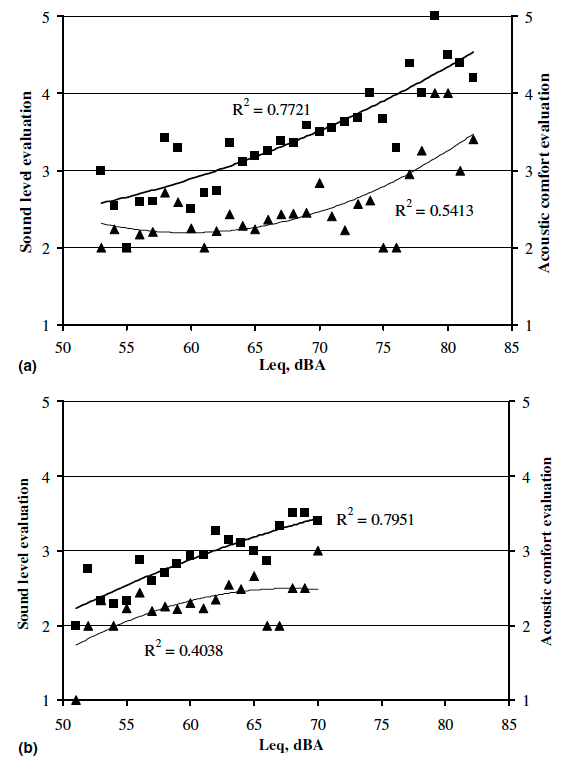
\includegraphics[width=.65\textwidth]{Figures/YangKang2005 Acoustic Comfort dB.png}
  \caption[Subjective responses and measured sound levels in urban spaces in Sheffield, UK.]{Reproduced with permission from \citep[Fig. 2]{Yang2005Acoustic} showing subjective responses and measured sound levels in urban spaces in Sheffield, UK. Relationships between the measured sound level, the mean subjective evaluation of the sound level and the mean acoustic comfort evaluation, with binomial regressions and correlation coefficients squared $R^2$. (a) The Peace Gardens. (b) The Barkers Pool. $\blacksquare$ -- subjective evaluation of sound level (1 [very quiet]; 2 [quiet]; 3 [neither quiet nor noisy]; 4 [noisy]; 5 [very noisy]). $\blacktriangle$ -- acoustic comfort evaluation (1 [very comfortable]; 2 [comfortable]; 3 [neither comfortable nor uncomfortable]; 4 [uncomfortable]; 5 [very uncomfortable]). \label{fig:yang2005acousticComfort} }
\end{figure}

\vspace{4mm}
\noindent\fbox{
    \parbox{\textwidth}{
      \vspace{-.25cm}
    \paragraph{Parallels in visual perception of green space}
    Similar results showing the disconnect between commonly used metrics of the physical environment and the environment's impact on the users have also been demonstrated by studies looking at visual perception. \citet{Kruize2019Exploring} demonstrated that the experience and use of natural urban spaces were strongly related to health outcomes associated with those spaces, while strictly physical characteristics of the space were not. 
    Their study made use of a cross-sectional design to investigate the relationships between several factors related to the experience of natural outdoor environments and key health outcome indicators. The outcome indicators investigated included physical activity, social contact, and mental health. As input indicators, they considered a set of GIS-derived quantitative indicators (i.e. \gls{ndvi}) \citep{Smith2017Characterisation} and a selection of metrics describing the use and experience of the space, derived from surveys of the study participants. These survey-derived experience metrics included \emph{perceived greenness}, \emph{satisfaction with the natural environment}, and \emph{importance of the natural environment}. Through multilevel regression analyses, the authors found that, in general, \gls{ndvi} was not statistically significantly related to increased physical activity or improved mental health, while perceived greenness, satisfaction with the space, and importance of the space were. A one point increase in perceived greenness (ranging from 0-12) was associated with an additional 10 min of physical activity per week and an increased mental well-being score (MHI-5) of 0.331 (range 8-100). 

    What is particularly interesting in these results is the difference in the findings between the objective measure of greenness and the perceived greenness. A study which used only the GIS-derived metric would have concluded that there was no relationship between greenness and the outcome factors. By including a perceptual attribute, \citet{Kruize2019Exploring} were able to demonstrate its importance. This suggests that what really matters to people's use of and the health and well-being impacts of these spaces is \emph{how they are perceived} more so than just what the physical characteristics are. 
    }
}


\paragraph*{}Across both the visual and the auditory domain, research has suggested that a disconnect exists between the physical metrics used to describe urban environments and how they are perceived. In addition, this disconnect can be extended further into how these environments influence the health and well-being of their users. To gain a better understanding of these spaces and their impacts on people who work and live in cities, we must create assessment methods and metrics which go beyond merely characterising the physical environment and instead translate through the users' perception. In order to make the case for why a new approach to perception-focussed assessment and design is necessary, we must first understand how the existing assessment methods have attempted to consider perception.


\section{Attempts to reconcile dB-focussed noise control with human perception}
In this section, I will begin with a brief discussion of the noise approach to annoyance and review some examples of noise assessment and mitigation methods and how they have attempted to reconcile the noted disconnect between the dB and the sound perception. This will provide the existing context for how traditional noise control approaches are targeted. 

\subsection{Assessing noise} In the UK, \citet{BS41422019} is the current reference document for assessing and addressing noise impacts in outdoor environments. In particular, BS 4142 is intended to assess the impact of a specific noise source when introduced to a given background level. BS 4142 makes use of a `rating level' based on a comparison between the sound which is being assessed and the background sound which would exist without it. Within the standard, a series of noise metrics are defined \citep[Sec. 3]{BS41422019}:

\begin{itemize}
  \item \textbf{ambient sound level, $L_a = L_{Aeq,T}$} - equivalent continuous A-weighted sound pressure level of the totally encompassing sound in a given situation at a given time, usually from many sources near and far, at the assessment location over a given time interval, \emph{T}.
  \item \textbf{background sound level, $L_{A90,T}$} - A-weighted sound pressure level that is exceeded by the residual sound at the assessment location for 90\% of a given time interval, \emph{T}, measured using time weighting, \emph{F}, and quoted to the nearest whole number of decibels.
  \item \textbf{equivalent continuous A-weighted sound pressure level, $L_{Aeq,T}$} - value of the A-weighted sound pressure level in decibels of continuous steady sound that, within a specificed time interval, $T = t_2 - t_1$, has the same mean-squared sound pressure as a sound that varies with time, and is given by the following equation:
  \begin{equation}
    L_{Aeq,T} = 10 lg_{10} \left[\frac{1}{T} \int^{t_2}_{t_1} \frac{p_A(t)^2}{p_0^2}dt \right]
  \end{equation}
    where: \\
      \space $p_0$ is the reference sound pressure (20 $\mu Pa$); and\\
      \space $p_a{t}$ is the instantaneous A-weighted sound pressure (Pa) at time \emph{t}
  \item \textbf{residual sound level, $L_r=L_{Aeq,T}$} - equivalent continuous A-weighted sound pressure level of the residual sound\footnote{Ambient sound remaining at the assessment location when the specific sound source is suppressed to such a degree that it does not contribute to the ambient sound.} at the assessment location over a given time interval, \emph{T}.
  \item \textbf{specific sound level, $L_s=L_{Aeq,Tr}$} - equivalent continuous A-weighted sound pressure level produced by the specific sound source at the assessment location over a given reference time interval, $T_R$.
\end{itemize}

In each of these metrics, the primary sonic feature which is assessed is the sound level, with some consideration for frequency content by using A-weighting. The standard then sets out the procedure to be used to measure the existing background sound level, measure or estimate the level of the specific sound, and calculate the margin between the specific sound and the background sound level. Throughout this process, BS 4142 notes `certain acoustic features can increase the significance of impact over that expected from a basic comparison between the specific sound level and the background sound level.' To address this, it introduces certain methods to add a character correction to the specific sound level, resulting in the rating level:

\begin{itemize}
  \item \textbf{rating level, $L_{Ar,Tr}$} - specified sound level plus any adjustment for the characteristic features of the sound
\end{itemize}

The sonic characteristics included for these rating level adjustments are tonality, impulsivity, intermittency, and `other sound characteristics' (described as `otherwise readily distinctive against the residual acoustic environment'). As an example of how these adjustments are applied, I will quote the guidance to adjust for tonality:
%\citep[pg. 13]{BS41422019}:

\begin{quote}
  \textbf{Tonality} \\
  For sound ranging from not tonal to prominently tonal the Joint Nordic Method \citep{ISO1996Part1} gives a correction of between 0 dB and + 6 dB for tonality. Subjectively, this can be converted to a penalty of 2 dB for a tone which is just perceptible at the noise receptor, 4 dB where it is clearly perceptible, and 6 dB where it is highly perceptible.
      \begin{flushright}
    \citet[pg. 13]{BS41422019}
  \end{flushright}
\end{quote}

The goal of these rating level adjustments is to incorporate aspects of the specific perception of sound, which may make a sound more disturbing, more noticeable, or generally more impactful than the dBA value alone would suggest. This is an important part of rating the impact of these sounds and necessary to achieve the goals of the standard. However, by implementing this as adjustments in terms of dB, it still centres the sound level in the assessment and enables only a one-dimensional approach to assessing impact. 

While BS 4142 is targeted towards assessing the impact of a specific sound, and primarily in an industrial and commercial context, \citet{ISO1996Part1} is more general, including provisions for assessing `community noise'. In the Introduction to the standard, several acknowledgements are raised about the importance of human perception, but the primary focus on the sound level is confirmed:

\begin{quote}
  To be of practical use, any method of description, measurement, and assessment of environmental noise is intended to be related in some way to what is known about human response to noise. [\ldots] The methods and procedures described in this part of ISO 1996 are intended to be applicable to noise from various sources, individually or in combination, which contribute to the total exposure at a site. At the stage of technology at the time of publication of this part of ISO 1996, the evaluation of long-term noise annoyance seems to be best met by adopting the adjusted A-weighted equivalent continuous sound pressure level, which is termed a ``rating level''. 
        \begin{flushright}
    \citet{ISO1996Part1}
  \end{flushright}
\end{quote}

Despite the nods toward a perception-focussed approach, ISO 1996 re-emphasises the focus on sound pressure level when it comes to discussing community noise annoyance:

\begin{quote}
  If the sound has special characteristics, then the rating equivalent continuous sound pressure level shall be the primary measure used to describe the sound. [\dots] research has shown that different transportation sounds or industrial sounds evoke different community annoyance responses for the same A-weighted equivalent continuous sound pressure level.
        \begin{flushright}
    \citet[Sec. 6.1]{ISO1996Part1}
  \end{flushright}
\end{quote}

What this review of some of the relevant standards and guidance demonstrates is that the decibel (specifically the equivalent continuous sound pressure level) is the dominant rating metric for all types of environmental noise and that, despite attempts to incorporate adjustments for `special' characteristics of the sound, the only sonic characteristic really being considered is the sound level. In addition, what my review of this guidance reveals is that the rating level adjustments are impractical to apply to complex sound environments for general evaluation. \citet[Eq. 4]{ISO1996Part1} provides a formula for calculating the rating level of combined sources:

\begin{equation}
L_{Req,T} = 10lg \left(\frac{1}{T} \sum_n \sum_j T_{nj} * 10^{0,1L_{Reqj,Tnj}}  \right) dB
\label{eqn:iso1996Rating}
\end{equation}
where

$$
T = \sum_n T_{nj}
$$

for each source \emph{j}.

However, ISO 1996 notes that `As a practical matter, [\cref{eqn:iso1996Rating}] is typically evaluated one source at a time.' This makes it clearly impractical as a method for assessing a general sound environment, with multiple competing sound sources, or for automated monitoring. In this way, these standards preclude the possibility of making use of the rating level to provide a more nuanced view of a sound environment which accounts for the sonic characteristics. 

\subsection{Community noise annoyance}
There is an existing methodology to address community noise annoyance, which began to develop in the 1940s following an increase in community complaints, primarily in response to aircraft noise \citep{Kryter1994}\footnotemark{}. From this, definitions of noise annoyance and single-number assessment indices were developed which focussed on the aircraft and transport noise impacts on residential areas. \citet{ISO15666} defines annoyance (specifically `noise-induced annoyance') as `one person's individual reaction to noise.` This is assessed through socio-acoustic surveys using questions with either verbal or numerical rating scales. In contrast to many studies from the soundscape literature, the noise annoyance scales in \citet{ISO15666} refer to long time scales (`Thinking about the last (12 months or so) \ldots') whereas soundscape studies have tended to focus on shorter and more immediate time scales \citep{Yang2013Psychoacoustical,Rychtarikova2013Soundscape}. This is perhaps due to the more complex nature of the perception under investigation in soundscape. 

\citet{ISO15666} then extends to \emph{community noise annoyance}, defined as `the prevalence rate of this individual reaction in a community as measured by the responses to questions specified in Clause 4 and expressed in appropriate statistical terms.' This approach to community noise inherently recognises that 1) noise annoyance is an individual response which will vary among people and 2) the most appropriate way to discuss this impact on a broader scale is to describe the aggregate response statistically (e.g. 80\% prevalence of `highly annoyed' individuals).

A commonly used metric in noise annoyance studies in this context is the \gls{ldn}, which is the average of the sum of the A-weighted sound energy over 24 hours, with a penalty of 10 dB added for the hours from 10:00 pm to 7:00 am, on an annualised basis \citep[pg. 571]{Kryter1994}:

\begin{dmath}
  L_{dn} = 10 log((1/54,000 (10^{L_{A}1s,7am..L_A1s,10pm/10})\\ + (10(1/32,400 (10^{L_A1s,10pm..L_A1s,7am/10}))
\end{dmath}


In the contexts for which it was developed, \gls{ldn} provides a good correlation with `the cumulative percentage of people' being moderately, very, or highly annoyed for specific sources of noise, such as aircraft noise (0.89, 0.89, and 0.87, respectively) \citep{Kryter1994}. A predictive trend curve can be derived from this:

\begin{equation}
\% \text{Highly annoyed} = 110.091 + (-5.023 \times L_{dn}) = (0.058 \times L_{dn}^2)
\end{equation}

However, as noted, this is employed for assessing the annualised annoyance from a specifically noted source averaged over 24 hours in a residential setting. The residential setting is particularly noted in the inclusion of the 10 dB penalty during night-time hours, to consider sleep disturbance impacts. The long time-scales and lack of consideration of either more complex sonic characteristics or the potential positive impacts of sounds make these methods unsuitable for assessing the soundscape of public spaces. However, noise annoyance methodology does provide a valuable advantage for our purposes when compared to the environmental noise assessment methods reviewed earlier:

\begin{quote}
  The procedures for estimating subjective annoyance and complaints about environmental noise are intended for the assessment of the reactions of large groups or neighborhoods of people, and not specific individuals within a group.
  \begin{flushright}
    \citet[pg. 571]{Kryter1994}
  \end{flushright}
\end{quote}

This concept will be further explored and addressed in \cref{ch:ProbabilisticPOC}.

\footnotetext{\citet{Kryter1994} opts not to refer to annoyance when referring to a single sound, in order to `avoid some of the ambiguity possible with the word \emph{annoyance}'. Instead, the author prefers to use the phrase \emph{perceived noisiness}, defined as `the subjective unwantedness felt from a sound, independently of any meanings or effects it may have.' I find this a somewhat strange definition, due to the specific attempt to define it independent of any meaning or effects. Whether someone considers a particular sound to be \emph{noise} could be entirely dependent on the meaning they associate with it and independent of the acoustical characteristics of the sound.} 

\paragraph*{} Traditional noise control methods face several challenges in decreasing noise pollution in modern cities. In many cases, these challenges stem from an approach focussed strictly on decreasing the noise levels or noise exposure in a given space. Part of this approach stems from traditional assessment methods which centre the sound level as the sole metric and which struggle to account for additional sonic characteristics such as tonality or the meaning associated with a sound. In particular, the metrics used, particularly when attempting to adjust for these characteristics, are impractical to apply for complex sound environments\footnote{Throughout this thesis, I will use the phrase `complex sound environment' or `complex soundscape' to refer to a real-world environment with overlapping and competing sound sources which consist of sonic characteristics that any single metric currently struggles to encapsulate.} with several overlapping sound sources. This approach can often prove impractical in situations where a problematic noise source cannot be moved or decreased, or where mitigation methods such as building a sound wall to block the sound transmission are expensive, infeasible, or undesirable \citep{Ekici2003Review}. This can result in many urban spaces which are intended to provide a restorative space in the city being unpleasant due to the unwanted noise and going underutilised with little way to address the issue. Where noise and acoustics is considered by planners and architects, their concern is typically with compliance of ordinances and regulations, or with maintaining the existing environmental conditions. Noise mitigation efforts frequently fail to centre human perception within the design \citep{Coelho2016Soundscape}. 

As can be seen in the structure and guidance of these standards documents, the goal is to maintain the existing sound environment and mitigate noise impacts from newly introduced sounds, with the dB, in terms of a rating level, as the metric of assessment. Attempts have been made across the various standards to include adjustments for how sonic characteristics such as tonality, impulsivity, and spectral content influence human perception in a useful and practical way. It should also be clear that, as expressed by Axelsson \proof{\citep{Axelsson2020Soundscape}}, these standards approach sound reactively, addressing it only as something to be managed, reduced, or tracked. Although the goals laid out in the \gls{end} have shown a shift to considering sound as a potential benefit to be protected and promoted, the assessment methods available are still rooted in the waste management approach. 

\subsection{Soundscape: A perception approach}

Soundscape studies strive to understand the perception of a sound environment, in context, including acoustic, (non-acoustic) environmental, contextual, and personal factors. These factors combine together to form a person's soundscape perception in complex interacting ways \citep{Berglund2006Tool}. Humans and soundscapes have a dynamic bidirectional relationship -- while humans and their behaviour directly influence their soundscape, humans and their behaviour are in turn influenced by their soundscape \citep{Erfanian2019Psychophysiological}. Researchers in the areas of acoustics, environmental psychology, and auditory neuroscience outline the adverse impact of noise or negative sounds on well-being in an attempt to improve modern living standards \citep{Ising2004Health,Lawton2016Living,Pedersen2007Wind,Hao2016Assessment}. In this regard, evidence indicates that positively perceived sounds (e.g. natural sounds) are associated with a high quality of life and enhanced psychological and physical health \citep{Alvarsson2010Stress,Aletta2018Associations,Jeon2010Perceptual,Shepherd2013Do}.

When applied to urban sound and specifically to noise pollution, the soundscape approach introduces three key considerations beyond traditional noise control methods:

\begin{enumerate}
  \item considering all aspects of the environment which may influence perception, not just the sound level and spectral content;
  \item an increased and integrated consideration of the varying impacts which different sound sources and sonic characteristics have on perception; and
  \item a consideration of both the positive and negative dimensions of soundscape perception. 
\end{enumerate}

This approach can enable better outcomes by identifying existing positive soundscapes (in line with the \gls{end}'s mandate to `preserve environmental noise quality where it is good' \citep{Directive200249ECEuropeanUniEuropean}), better identify specific sources of noise which impact soundscape quality and pinpoint the characteristics which may need to be decreased, and illuminate alternative methods which could be introduced to improve a soundscape where a reduction of noise is impractical \citep{Kang2018Impact,Fiebig2018Does}. These can all lead to more opportunities to truly improve a space by identifying the causes of positive soundscapes, while also potentially decreasing the costs of noise mitigation by offering more targeted techniques and alternative approaches.


\section{Soundscape studies}
This section will review the terms used for defining soundscapes, some existing methods for characterising urban soundscapes, and the previous attempts and frameworks for connecting the physical environment with soundscape perception.

Soundscape, conceived as the acoustic equivalent of landscape, is defined as the human's perception of the acoustic environment, in context \citep{ISO12913Part1,Kang2010understanding,SoundscapeOursonicSchafer}. The soundscape can be the result of a single sound or a combination of sounds that arises from an engaging environment. The Canadian composer and naturalist R. Murray Schafer led much of the original work to advance research in the area \citep{Schafer1969New}, borrowing the term originally from work carried out by city planner Michael Southworth \citep{Southworth1969sonic}. Since Schafer, there have been several multi-dimensional classifications for soundscapes. However, according to Schafer, the main components of the soundscape consist of keynote sounds, sound signals, and soundmarks. The soundscape ecologist Bernie Krause characterised soundscapes into three main domains based on the source of the sound. According to his classification, the soundscape refers to a wide spectrum of sounds, encompassing natural sounds relating to non-organic elements of nature such as waterfalls (geophony), organic but non-human sources such as animals' copulatory vocalisations (known as biophony), and all environmental sounds generated by human sources (anthrophony) such as human voices or human activity-related sounds \citep{Krause1987WholeEarth,Kang2016}. From this starting point in music and soundscape ecology, urban soundscape studies have advanced over the last two decades \citep{Kang2006Urban,Kang2018Impact}. \citet{Fiebig2018Does} noted that the standardization of soundscape methods was necessary to provide `minimum measurement requirements leading to a (minimal) guaranteed level of reliability'. The next section will review the history and outcome of the resulting standard.

% \draft{Need contextual sentences for the following paragraphs}
% \paragraph*{Quiet Areas}
% The concept of defining quiet areas maintains a focus on `identifying and preserving quiet areas' \citep{EEA2020Environment} following the imperative given in the \gls{end} \citep{EU2002Directive}. This approach is mostly rooted in a noise mindset, although the methods employed for identifying quiet areas vary across countries within the EEA. Background sound levels seem to play an important role in identifying quiet areas, in particular when attempting to produce maps of available quiet areas on a city- or agglomeration-scale such as that used in the \citet{EEA2020Environment}, where quiet areas were defined as: "those with less than 55 dB $L_{den}$ from road, rail, aircraft and industrial sources and were classified, depending on their land cover type, as quiet areas with green/blue land cover." However, several background noise thresholds are cited as being used by agglomerations for their definitions, along with non-acoustic criteria such as urban functionality, land cover type, location, size and accessibility of the area, visual qualities, and subjective judgement. 
% Despite these attempts to incorporate multiple factors within the definition of quiet areas, this approach still tends toward a 1- or 2-dimensional focus, and struggles to take a holistic approach to people's perception or response to the space.

% Given that the Quiet Areas approach started with the 2002 \gls{end}, predating the ISO 12913 series of technical specifications on soundscape, it has not yet moved in line with the conception of `soundscape' and the accompanying measurement methods and reporting requirements given in the ISO documents. There is therefore an open question of whether the directive to identify and preserve quiet areas would truly be considered soundscape, however it does represent the most successful foray into policy and is frequently cited as a success by soundscape researchers \cit{Aletta, Guastavino, Kang, etc.}.

% \paragraph*{Sound Art / Installations}
% \draft{definition of sound art / installations}
% In \cit{Lacey2016SonicRupture}, the author presents sound art as a form of 'sonic rupture'. Drawing from Felix Guattari's \cit{Guattari} concept of ecological ruptures which `act to diversify affective potential within delimited environmental loci', sonic rupture provides the opportunity to disrupt the repetitive patterns of urban sound and induce a new -- or perhaps just a more interesting -- affective response. 

% In Lacey's practice, the starting point of thoughtful sound art is to enable `new expressions [to] emerge within the practicioner that provides the impetus to diversify a space's affective potential'. Lacey reiterates the bi-directional nature of people's relationship with the soundscape, stating `the environment affects the practicioner and the practicioner in turn affects the environment in which those who encounter the new environments realize new sensations and experiences'.

% In contrast to many other approaches to soundscape design, \cit{Lacey} makes it clear that all \dots

% Although the approach taken in sound art studies is often quite different from the engineering approach taken here, one point does carry through: 

% \begin{quote}
%   As will be made clear, the rupture does not judge noise; rather it recognizes noise as the ubiquitous environmental condition of the urban that must be diversified if the contemporary city is to afford creative encounters. 
% \end{quote}

% It is this treatment of \emph{noise} which can be brought into an engineering approach. Where the term noise is specific, referring only to unwanted sound, \emph{urban noise} is often used in a broad-ranging way. It is taken to encapsulate all of the overlapping, competing, and ever-present sounds which emerge from urban life. Many of these may in fact be noise, but to cast all repetitive or idiomatic urban sounds as noise dismisses the potential of this urban roar to be more than just noise and, in fact, it dismisses the idea that individuals can all have their own perception and response to these sounds, where they may not consider them as `noise'. Both the sonic rupture and the soundscape engineering approaches take amore nuanced approach which expands the possibilities for how people perceive urban sound and how these environments may be treated.


%%%%%%%%%

\subsection{Standardising Soundscape: The ISO 12913 series}
The soundscape community is undergoing a period of increased methodological standardization in order to better coordinate and communicate the findings of the field. This process has resulted in many operational tools designed to assess and understand how sound environments are perceived and apply this to shape modern noise control engineering approaches. Important topics which have been identified throughout this process are soundscape `descriptors', `indicators', and `indices'. \citet{Aletta2016Soundscape} defined soundscape descriptors as `measures of how people perceive the acoustic environment' and soundscape indicators as `measures used to predict the value of a soundscape descriptor'. Soundscape indices can then be defined as `single value scales derived from either descriptors or indicators that allow for comparison across soundscapes' \citep{Kang2019Towards}.

This conception has recently been formalized and expanded upon with the adoption of the recent ISO 12913 set of standards \citep{ISO12913Part1, ISO12913Part2,ISO12913Part3}. ISO 12913 Part 1 sets out the definition and conception of soundscape, defining it as the `acoustic environment as perceived or experienced and/or understood by a person or people, in context'. Here, the soundscape is separated from the idea of an acoustic environment, which encompasses all of the sound which is experienced by the receiver, including any acoustically modifying effects of the environment. In contrast, the soundscape considers the acoustic environment, but also considers the impact of non-acoustic elements, such as the listener's context and the visual setting, and how these interact with the acoustic environment to influence the listener's perception.


\subsection{A note on terminology: Soundscape Perception?}
\label{sec:terminology}

According to the definition of soundscape provided in \citet{ISO12913Part1}, the soundscape is `the acoustic environment as perceived or experienced and/or understood by people'. Both in the standard and elsewhere, this has commonly been taken to mean that the soundscape is the perception itself, while the factors which lead to the soundscape are separate entities. The beginning of this definition of soundscape as perception can be found in \citet{Truax1999Handbook} as `an environment of sound with emphasis on the way it is perceived and understood by the individual, or by a society'. This definition was further developed by \citet{Brown2012review} (and adopted into \citet{ISO12913Part1}) to mean that the soundscape is not made up of sound sources, the sound environment, etc. but instead is the perception formed by them. Brown made this distinction very clear in a section titled \textbf{`Soundscape is perception of the acoustic environment of a place'}: `Thus, a soundscape exists through human perception [\ldots] the soundscape of a place is thus a perceived entity'.

Given this definition, speaking about the `soundscape perception' would be redundant; the soundscape already is the perception. By extension, saying `the soundscape is perceived as pleasant' also would not make sense; we should rather say `the soundscape is pleasant'. However, even among the foundational modern soundscape literature this use is relatively widespread; \citet{Axelsson2010principal} and \citet{Liu2014Effects} both refer to soundscape perception within the title. 

This definition also conflicts with other popular definitions of soundscape. The term soundscape is commonly used in acoustic ecology and underwater acoustics -- see titles such as `The soundscape of bat swarms' \citep{Kloepper2017soundscape}, `An integrated underwater soundscape analysis in the Bering Strait region' \citep{McKenna2021integrated}, `Soundscape analysis and acoustic monitoring document impacts of natural gas exploration on biodiversity in a tropical forest' \citep{Deichmann2017Soundscape}, and `Identification and quantification of soundscape components in the Marginal Ice Zone' \citep{Geyer2016Identification}. Several analysis packages have also been developed for the purpose of soundscape analysis, whether for urban-, underwater-, or bio-acoustics, which include no aspect of human perception in context (see e.g. Soundscape Viewer \citep{Sun2020Soundscape} and \texttt{scikit-maad} \citep{Ulloa2021scikit}). 

These fields appear to use the term \emph{soundscape} more broadly, without a reference to human perception, to refer to either a broad consideration of the entire sound environment or to a focus on the sound environment as experienced by all creatures, not just humans. This first definition comes from \citet{Pijanowski2011Soundscape} where the authors state that `soundscape ecology focuses mostly on macro or community acoustics [\dots] the composition of all sounds heard at a location that are biological, geological, or anthropogenic' to differentiate it from previous acoustic ecology studies which `focus on a single species or a comparison of species'. Within the ISO 12913 framework, this would more accurately be described as the \emph{acoustic environment} (`sound at the receiver from all sound sources as modified by the environment'). In the end, all of these conflicting and overlapping definitions can make cross-disciplinary communication more difficult and prone to disagreements and misunderstandings. 

In an attempt to bring the term soundscape in line with these varying uses and to conform more broadly with its common grammatical usage, I propose the following definition:

\begin{quote}
The soundscape comprises all of the factors which influence the sonic experience or perception of an environment; this primarily includes the acoustic environment, composed of all sounds heard at a location that are biological, geological, technological, or anthropogenic. The secondary factors included in the soundscape are those non-auditory factors which influence how the sound environment is processed, including (but not limited to) the visual setting, environmental factors, and the internal, personal factors 
which mediate the listeners' perception.
\end{quote}

This definition draws from both the definition of acoustic environment given in \citet{ISO12913Part1} and on the use in soundscape ecology as given by \citet{Pijanowski2011Soundscape}. It reflects the holistic view of soundscape analysis which aims to consider more than the sound environment alone and also consider how non-acoustic factors impact how sound environments impact listeners. In urban and human soundscape studies, like this thesis, the investigation and understanding of the soundscape is focussed on human perception as in \citet{ISO12913Part1}. In soundscape ecology, it reflects the desire to consider sources from many species, including anthropogenic sources, and especially to focus on the impact on the animals and ecological systems. A scientific consensus of what constitutes the definition of the secondary, non-acoustic factors is still being developed, notably as a proposed ISO Technical Specification \citep{Fenech2021Development}. A preliminary definition of non-acoustic factors was proposed by \citet{Riedel2021Considering} as:

\begin{quote}
  All factors other than the objective, measured, or modelled acoustic parameters which influence the process of perceiving, experiencing and/or understanding an acoustic environment in context, without being part of the causal chain of this process.
\end{quote}

While this preliminary definition very closely fits the conception of non-acoustic factors used throughout this thesis, it misses one key aspect. As illustrated in \cref{fig:percepMap} and empirically demonstrated in \cref{ch:mlmann}, the semantic meaning attached to sound sources is an important factor in the formation of a soundscape perception. This information is directly tied to the sound source, and is in some way acoustic, but it would not fall into the `objective, measured, or modelled acoustic parameters' definition. Sound source information would therefore fall into some limbo space between `acoustic' and `non-acoustic' factors under Riedel's definition. Some revision may need to be made to rectify this and clarify whether sound source semantic information should be considered as part of the acoustic factors. For this reason, my proposed definition has used the term `non-auditory factors' to avoid the discrepancy.

This usage also seems to be more readily understood by lay-people. Explaining that the soundscape \emph{is} the perception, not something which can be perceived, seems to raise an unnecessary barrier to effective communication. In contrast, when explaining a soundwalk to a participant, with this definition we could say ``I'd like you to think about the soundscape of this space -- not just the sounds you can hear but also the context you're hearing them in. Then tell me how you perceive that soundscape, is it pleasant, calm, etc.?" Removing the somewhat awkward idea of the soundscape is the perception, could aid in the communication of the soundscape to the public.

%%%%%%%%%%%%%%%%%%%%%%%%%%%%%%%%%%%%%%

\subsection{Soundscape data collection methods}
Methods for collecting data on how people experience acoustic environments have been at the forefront of the debate in soundscape studies for the past 20 years. While the soundscape research field as we understand it today dates back to the late 1960s with the pioneering work of authors like M. Southworth \citep{Southworth1969sonic}, R.M. Schafer \citep{SoundscapeOursonicSchafer}, and H. Westerkamp \citep{Westerkamp2002Linking}, the theme of data collection methods for soundscape assessment emerged more prominently only recently \citep{Kang2016Ten}. There is a general consensus in the research community that standardised tools to gather and report individual responses on the perception of urban acoustic environments are indeed desirable, to provide comparable datasets and soundscape characterisations across different locations, times, and samples of people, as well as allowing for replicability studies and offering inputs for modelling algorithms in soundscape prediction and design tasks. These were among the main drivers for the establishment of a Working Group at the \gls{iso} back in 2008, which was named `Perceptual assessment of soundscape quality' (ISO/TC 43/SC1/WG 54) that has so far published three documents within the ISO 12913 series on soundscape. Part 1 (ISO 12913-1:s014) is a full standard and provides a general framework and definitions of soundscape concepts \citep{ISO12913Part1}, while Part 2 (ISO/TS 12913-2:2018) and Part 3 (ISO/TS 12913-3:2019) are technical specifications which offer guidance on how data should be collected and analysed, accordingly \citep{ISO12913Part2,ISO12913Part3} (Part 4, on soundscape design interventions, is currently under development by the working group, also registered as a technical specifications document). Specifically, Part 3 presents the proposed methods for analysing and representing the data collected by the soundscape surveys. Since the development of these standards, the focus has shifted from understanding individual perception to characterising the collective perception of increasingly large groups.

The ISO/TS 12913-2:2018 is the current reference document addressing data collection and reporting requirements in soundscape studies. In terms of methods, the ISO document covers two main approaches, namely: soundwalks combined with questionnaires (Methods A and B) and narrative interviews (Method C) \citep{ISO12913Part2}, which relate to on-site and off-site data collection, accordingly. Part 3 of the ISO 12913 series builds on Part 2 and provides guidelines for analysing data gathered using only those methods \citep{ISO12913Part3}. However, the range of possible methodological approaches to soundscape data collection is much broader and it includes, for instance, laboratory experiments \citep{Aletta2016Soundscape,Sun2019Classification,Oberman2018Towards}, pseudo-randomized experience sampling \citep{Craig2017Experience}, and even non-participatory studies \citep{Lavia2018Non}. 


% \paragraph*{Soundwalks}
% Lit review of the concept of soundwalks
% Soundwalks, following \gls{wsp} have focussed on the soundscape as 1) an individual's experience of a particular space or 2) as the sonic expression of a culture or community's relationship with the space \citep{Droumeva2021sound}. Starting with Schafer's framing of the soundscape as a collective composition balancing background and foreground sounds, soundmarks and primary sound types, to the \gls{iso} definition of a soundscape, the totality of the acoustic and contextual environment is processed and interpreted by an individual. Despite the \gls{iso}'s expansion from the individual to a group highlighted by the phrasing "by a person, or people", the tools it presents -- and, in particular, how they have been employed -- fail when attempting to address the perception of many people.

% This conceptual difficulty in dealing with the perception of many people has contributed to the problems associated with incorporating perception-focussed approaches in practice and regulation. \draft{A bit more on soundwalks as a method?} 

% In a recent editorial paper on Soundscape Assessment, Axelsson and colleagues observe that it is important to critically discuss current theories and models in soundscape studies and to examine their effectiveness, while also looking at how to integrate different methods and perspectives for the discipline to make further advancements \citep{Axelsson2019Editorial}. This work was mainly aimed at addressing the issue of meaningful comparability and representation of soundscape assessments. Part 2 of the ISO 12913 standard itself does not provide ultimate answers: the technical specifications recommend multiple methods, as consensus around a single protocol could not be reached. This diversity of methodological approaches should be interpreted as a fact that soundscape theory is still under development and, for this reason, the standardisation work should probably take a step back and focus on developing a reference method for comparability among soundscape studies, rather than a single protocol for soundscape data collection. Some attempts have indeed already been made in literature for the different methods proposed in the ISO/TS 12913-2:2018 \citep{Aletta2019Exploring, jo2020soundscape}.

% This study thus aims to review the consequences of these methods for larger datasets and provide concrete examples for how soundscapes should be represented. In particular, we aim to strengthen the practices for characterising the soundscape of a location, as a collective perception by the users of the location. We also demonstrate how the progress of these tools from their initial scope (measuring and discussing the individual perception of a soundwalk participant) have not kept up with recent advances and requirements for larger-scale soundscape datasets. We question whether there are some issues related to the data collection instruments and data analysis methods as recommended, and examine the results of the model framework and mathematical transformations laid out in the ISO technical specifications in order to provide guidance on the interpretation of the soundscape circumplex.

%%%%%%%%%%%%%%%%%%%%%%%%%%%%%%%%%%

\section{Soundscape descriptors, indicators, and perceptual mapping}
\citet{Aletta2016Soundscape} provides a review of the soundscape descriptors and indicators commonly used in soundscape research and outlines an initial framework for developing predictive soundscape models. In their review, the authors identified eight potential soundscape descriptors:

\begin{enumerate}
  \item Noise annoyance
  \item Pleasantness
  \item Quietness or tranquility
  \item Music-likeness
  \item Perceived affective quality
  \item Restorativeness
  \item Soundscape quality
  \item Appropriateness
\end{enumerate}

To this list, `acoustic comfort' as used in \citet{Yang2005Acoustic} and \citet{Vardaxis2018Reviewa} could be added as a ninth potential descriptor. Similarly, the authors identified a range of potential indicators used to characterise the acoustic environment:

\begin{itemize}
  \item \gls{laeq}
  \item statistical levels ($L_x-L_{100-x}$)
  \item proportion of low-frequency sounds (\gls{lcla})
  \item Loudness (\gls{n5})
  \item Sharpness (\gls{s})
  \item Roughness (\gls{r})
  \item Fluctuation Strength (\gls{fs})
\end{itemize}

However, it is noted that several studies show that no single psychoacoustic indicator alone can explain the variation in soundscape responses (as expressed via the descriptors) (e.g. \citep{PerssonWaye2002Psycho}). The goal of statistical modelling, therefore is to create a more complex and complete representation of the relationship between soundscape indicators and descriptors, beyond what any single indicator could achieve. 

\begin{figure}[h]
  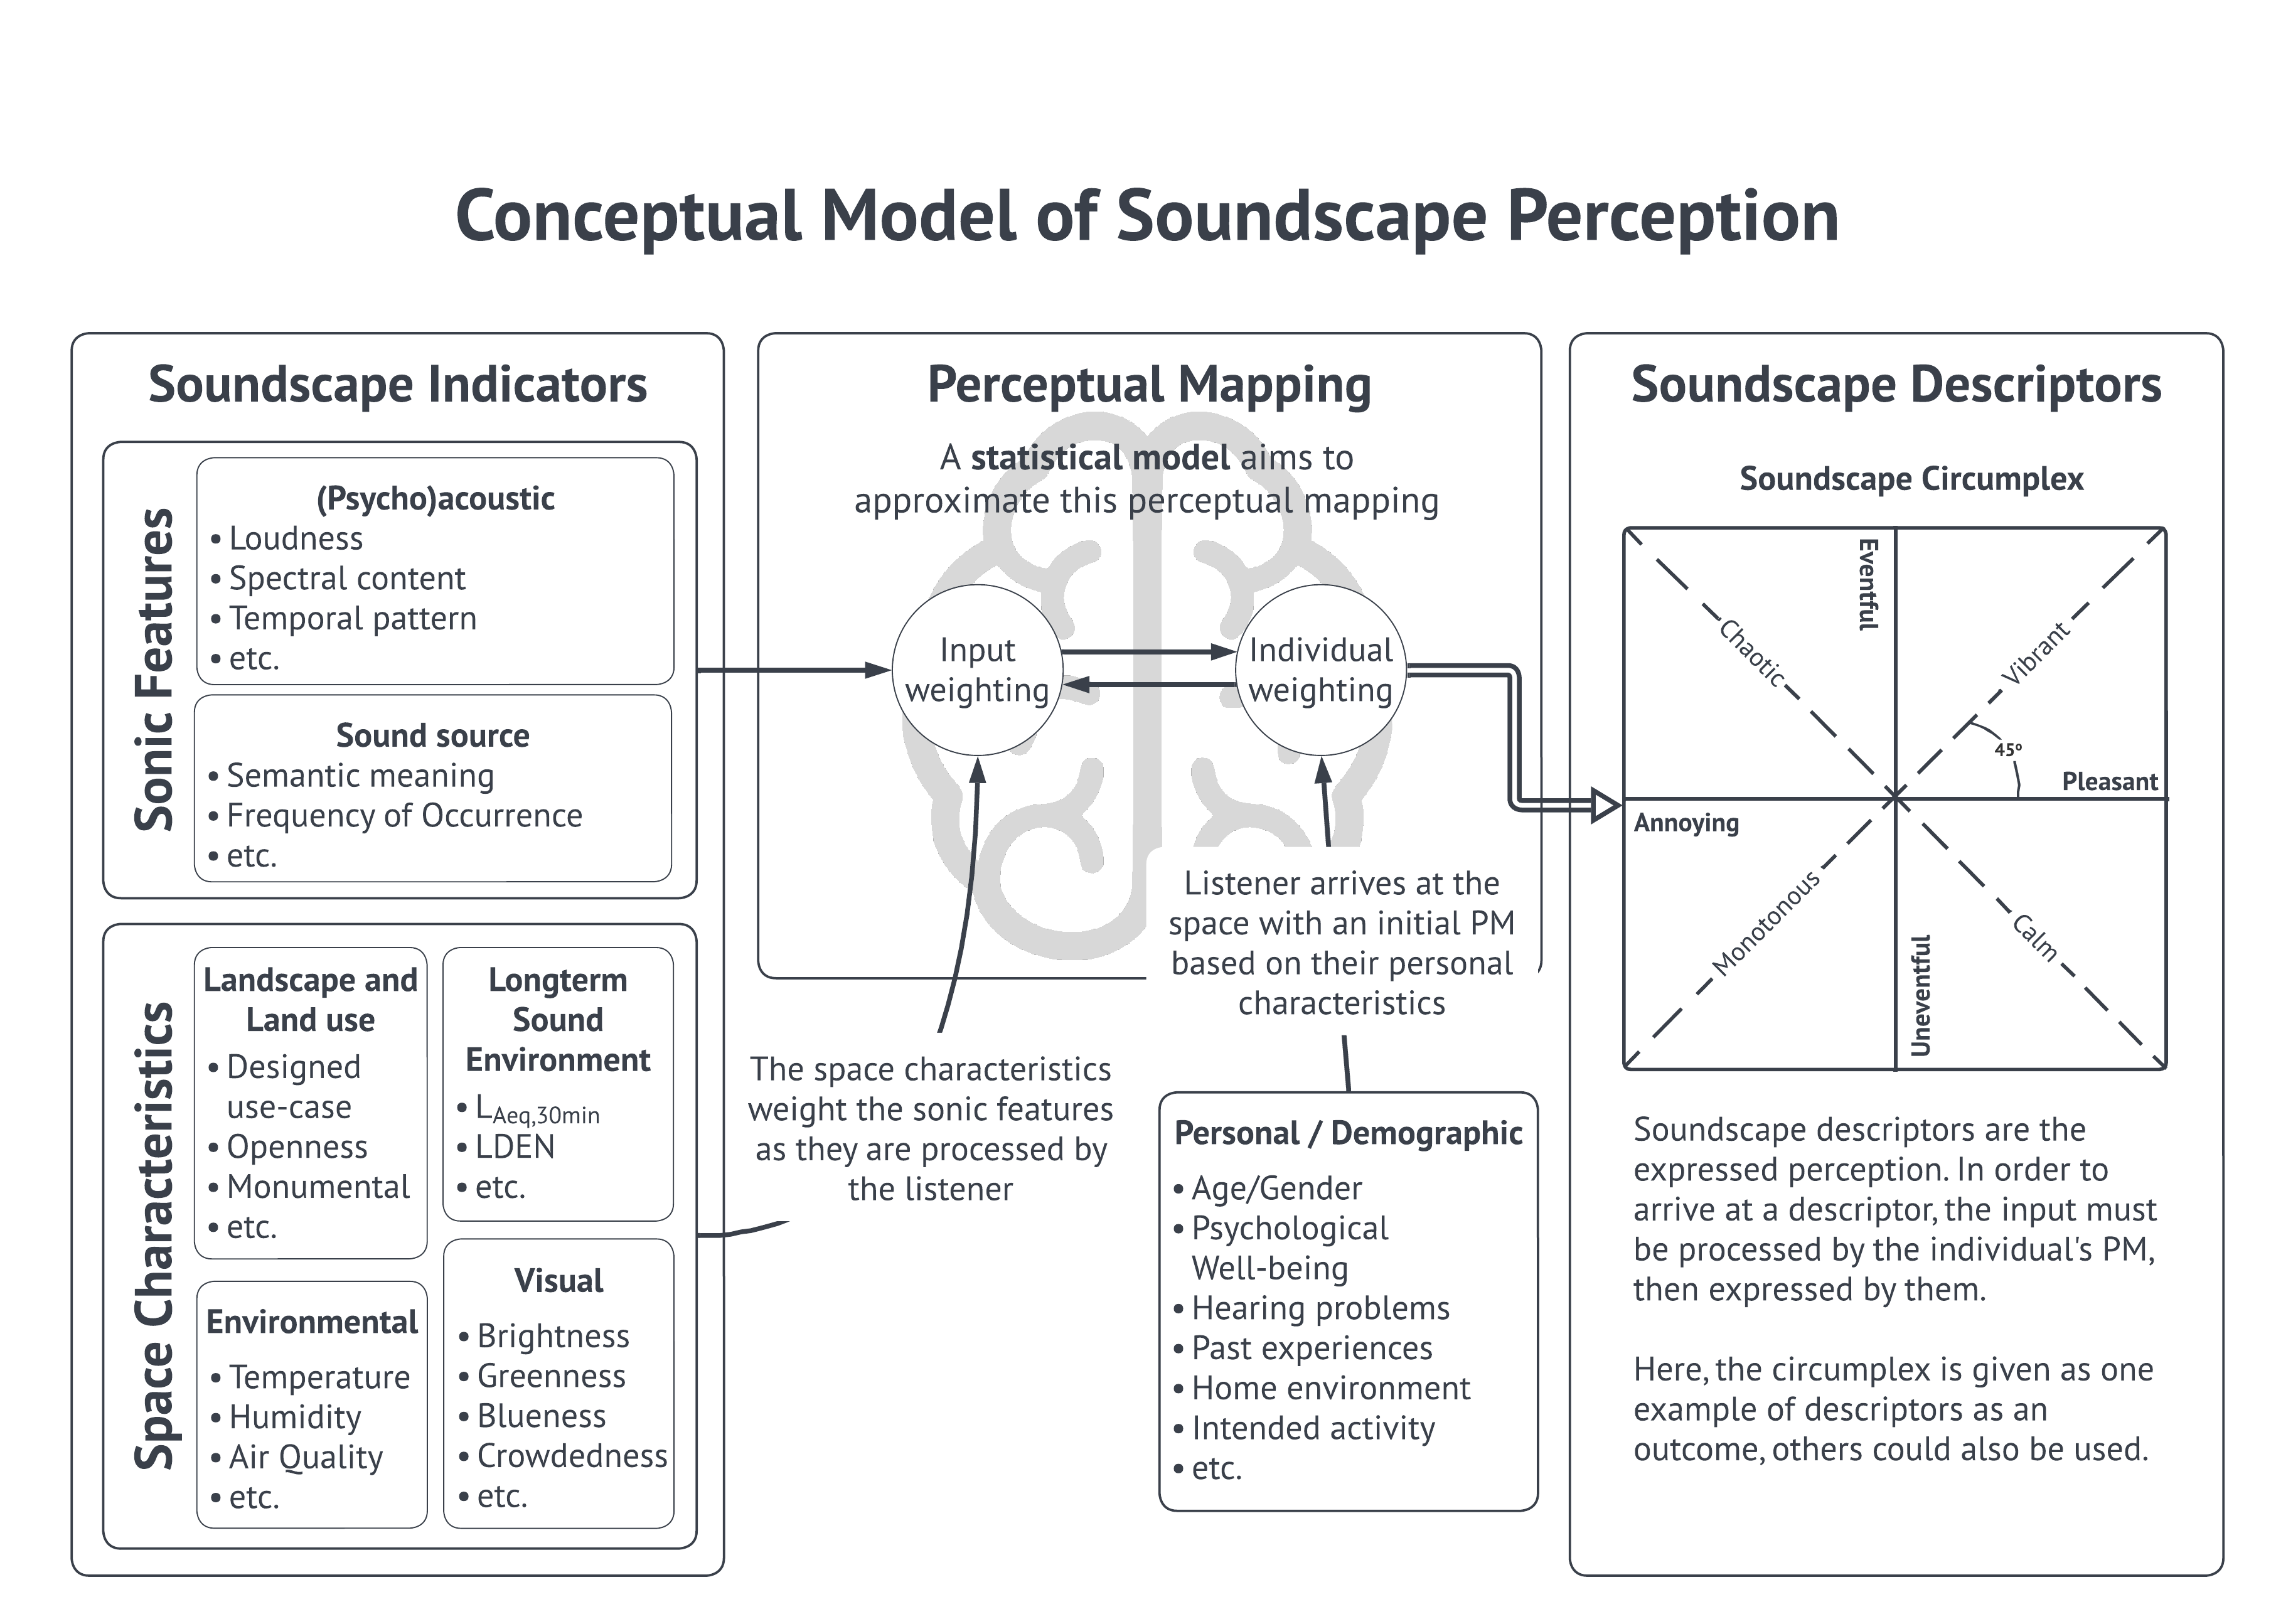
\includegraphics[width=\textwidth]{Figures/Overall Model Concept Diagram_2022-04-28.png}
  \caption{The conceptual model of soundscape perception, illustrating the perceptual mapping from physical inputs, through personal experience, to soundscape descriptors. The role of the statistical model is to attempt to approximate or reflect this perceptual mapping. \label{fig:percepMap}}
\end{figure}

\cref{fig:percepMap} shows a conceptual view of this relationship. We start with \textbf{soundscape indicators}, describing the physical environment to which a listener is exposed. Soundscape indicators characterise the physical and contextual environment to which the listener is exposed. This can be broken down into \textbf{sonic features} (e.g. the acoustical features listed above) and \textbf{characteristics of the space} itself (e.g. the amount of visible sky, the intended use-case of the space, how crowded the space is, etc.). In order to translate from the physical inputs to an expressed description of the soundscape perception, we introduce the concept of a \textbf{perceptual mapping} \citep{Lionello2021Thesis}. This mapping represents a simplified idea of how each individual's brain processes the inputs from the soundscape which they experience, forms a perception, and finally expresses that perception through their description of the soundscape. For our purposes, this perceptual mapping is treated as essentially a black box mapping inputs to outputs. It can be conceived of as a network of weights in which certain characteristics of the sound may have different weights and directions depending on the context, through which all of the inputs are processed, resulting in the soundscape rating. Conceptually, this perceptual mapping -- the pathways and weightings through which the inputs are processed before being expressed as a perceptual descriptor -- is established prior to an individual's exposure to the soundscape in question.

We then break the perceptual mapping into two parts: how the inputs are weighted relative to each other (which is relatively consistent across participants) and the particular variation in each person's perception based on their own experiences and background. In this conceptual model, the weighting of the sonic features (both the acoustic features and the sound source information) are mediated by the space characteristics as they are processed by the listener. The individual weightings represent the effects due to the listener's particular personal characteristics (their age, gender, psychological well-being, etc.) as well as the inherent unpredictable randomness in each individual's experience of the soundscape.  Following the definition of soundscape established in \cref{sec:terminology}, the `soundscape' would be the general term used to describe all of the inputs to the perceptual mapping while the outcome of the perceptual mapping is the soundscape perception, as expressed through soundscape descriptors.

It should be made clear that this represents a very simplified view of how a soundscape perception is formed, however it provides a useful conceptual framework for the purposes of understanding and modelling how someone's perception forms in response to their exposure to a space. One way to consider the function of a statistical model of soundscape perception is as replicating the perceptual mapping between soundscape indicators and descriptors \citep{Lionello2021Thesis}. As a person experiences an urban space, they are exposed to an array of physical inputs, these are then processed by the listener through their own personal experience and mapped to their perception of that space. This perception is then expressed through their description of this experience of the soundscape. It is this mapping of physical inputs to perceptual description which the statistical model aims to reflect. The most successful model would then accurately replicate the general perceptual mapping across the population.

% As will be expanded upon in \cref{sec:NeedForPredModels}, the core message of this thesis is the importance of developing models which can predict soundscape perception and be put to use in assessing urban soundscapes. \citet{Aletta2016Soundscape} crucially laid out a forward-looking framework for the terminology used in soundscape studies and how the development of predictive models can progress. The work presented in this thesis can be viewed as fulfilling the steps presented in that framework and further developing Aletta's ideas around the creation and uses of predictive modelling. In line with this, the following section will review \citet{Aletta2016Soundscape} in depth in order to clarify the background which led to the advancements presented in \crefrange{ch:lockdown}{ch:ProbabilisticPOC}.


% In order to consistently discuss soundscape and the factors which influence it, it is important to understand what terms have been used to describe soundscapes. Both the traditional focus on the epidemiological impacts of noise and the development of the soundscape concept have used many different terms in order to describe the perception of a sound environment. Following \citet{Aletta2016Soundscape}, I'll group these under soundscape descriptors. 


\subsection{Perceived affective quality}
\label{sec:paqReview}
Based on the work in \citet{Aletta2016Soundscape} and a recent review of predictive soundscape models \citep{Lionello2020systematic}, among the potential soundscape descriptors which can be used, I have selected the soundscape circumplex \citep{Axelsson2010principal}, specifically the version in Method A of \citet{ISO12913Part2}, as the most appropriate for predictive modelling. 

Method A is built on a series of descriptors referred to as the \glsfirst{paq}, proposed by \citet{Axelsson2010principal}. These \glsplural{paq} are based on the pleasantness-activity paradigm present in research on emotions and environmental psychology, in particular Russell's circumplex model of affect \citep{Russell1980circumplex}. As summarised by Axelsson: `Russell's model identifies two dimensions related to the perceived pleasantness of environments and how activating or arousing the environment is.' This circumplex model is formed of two dimensions, pleasantness (often referred to as valence) and activity (or arousal), which are orthogonal to each other. In their study, three primary dimensions of soundscape perception were extracted from participants' responses to complex sound samples measured on 116 attributes, using Principal Components Analysis. The first component was found to represent pleasantness (aligning with attributes such as comfortable, appealing, uncomfortable, disagreeable, and inviting) and explained 50\% of the variance in the dataset. The second component was found to represent eventfulness (eventful, lively, uneventful, full of life, and mobile) and explained 18\% of the variance. The third component was found to represent familiarity (commonplace, common, and familiar) and explained 6\% of the variance, however this third component is typically disregarded as part of the standard circumplex. As will be made clear throughout, the circumplex model has several aspects which make it useful for representing the soundscape perception of a space as a whole.

When applied to soundscape, Axelsson re-termed these main axes as `Pleasant' and `Eventful', and also identified a set of additional axes which are rotated 45° from the main axes. This rotated axis contains additional attributes which represent various mixtures of the pleasant and eventful attributes: `Exciting', `Chaotic', `Monotonous', and `Calm'. This circumplex model of soundscape can be seen in \cref{fig:circumplexOnly}. In Method A, these \glsplural{paq} are collected through a series of questions with 5-point Likert-type responses where participants are asked to what extent they agree or disagree that the present surrounding sound environment is pleasant, exciting, etc. for each of the 8 descriptors. Method A also includes questions on: the sound source composition of the space, broken down into `Traffic noise', `Other noise', `Sounds from human beings', and `Natural sounds'; overall soundscape quality; and appropriateness of the sound environment to the place. The circumplex model, along with the sound source and general soundscape questions represent a relatively comprehensive method for assessing the soundscape of a space.

\begin{figure}
  \centering
  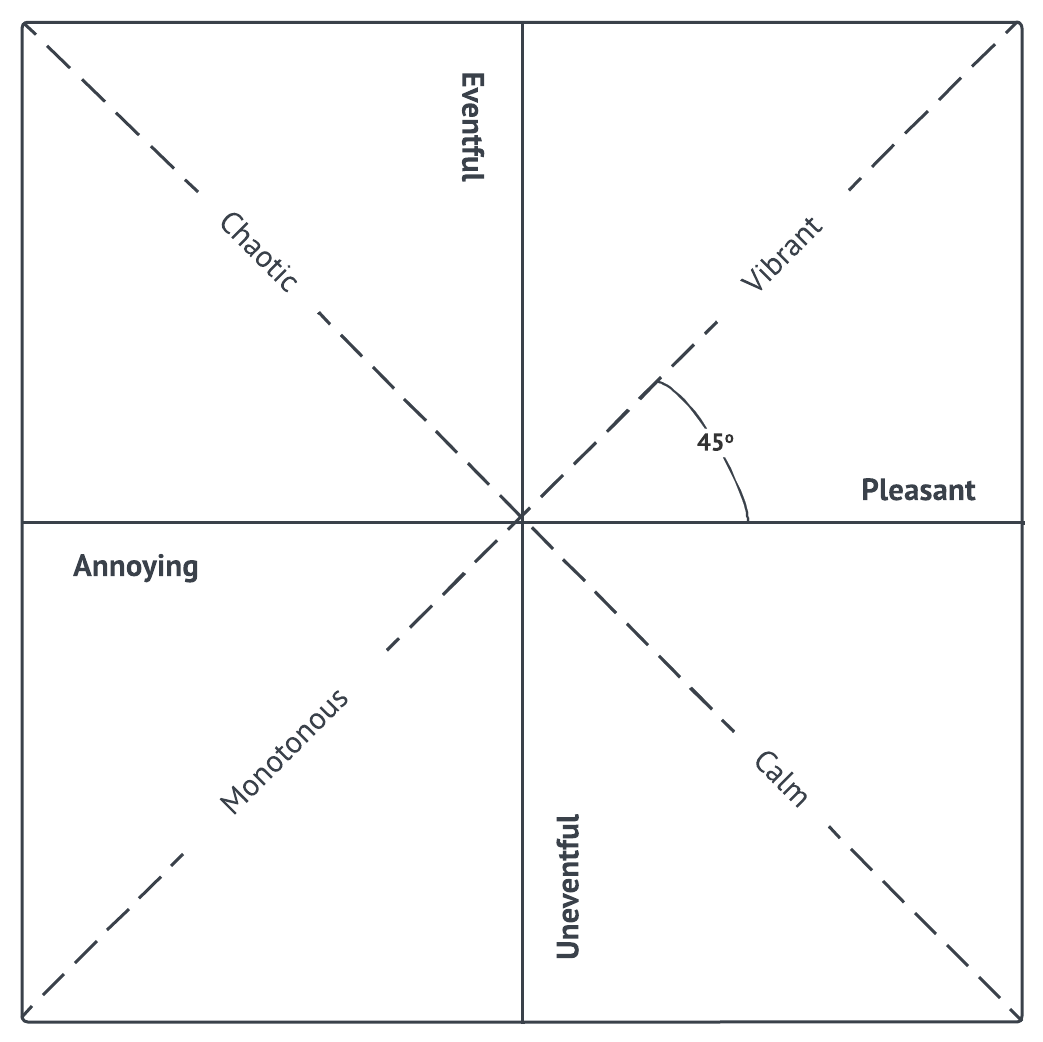
\includegraphics{Figures/CircumplexOnly.png}
  \caption{The soundscape circumplex, as originally derived by \citet{Axelsson2010principal} and updated in \citet{ISO12913Part2}. \label{fig:circumplexOnly}}
\end{figure}

One benefit of the circumplex model is that, as a whole, it encapsulates several of the other proposed soundscape descriptors - in particular, annoyance, pleasantness, tranquility, and possibly restorativeness \citep{Aletta2016Soundscape}. According to \citet{Axelsson2015How}, the two-dimensional circumplex model of perceived affective quality provides the most comprehensive information for soundscape assessment. It is also possible that the overall soundscape quality could itself be derived from the pleasant-eventful scores derived for a soundscape.

The circumplex also lends itself well to questionnaire-based methods of data collection, as proposed in \citet{ISO12913Part2}. In contrast to methods such as soundwalks, interviews, and lab experiments, in-situ questionnaires are able to provide the quality and amount of data which is necessary for statistical modelling. Large-scale, in-situ questionnaires are therefore considered the most appropriate data collection approach for generating a soundscape assessment database intended for predictive modelling. Combined, these factors make the circumplex the most appropriate method for predictive modelling as it provides a comprehensive summary of soundscape perception in a form which lends itself to machine learning model development.

\section{Statistical models of soundscape perception}
Several studies prior to the formalization of the ISO standards on soundscape demonstrated the general, but inadequate, relationship between traditional acoustic metrics, such as $L_{Aeq}$, with the subjective evaluation of the soundscape \citep{Berglund2006Tool,Yang2005Acoustic,Rychtarikova2013Soundscape,Aumond2017Modeling,AlsinaPages2021Perceptual}. These have typically aimed to address the existing gap between traditional environmental acoustics metrics and the experience of the sound environment. \citet{Yang2005Acoustic} showed that, when the sound level is `lower than a certain value, say 70 dBA', there is no longer a significant change in the evaluation of acoustic comfort as the sound level changes. However, the perceived sound level does continue to change along with the measured sound level, showing that (1) measured sound level is not enough to predict soundscape descriptors such as `acoustic comfort', and (2) there is a complex relationship between perceived sound level and soundscape descriptors which is mediated by other factors.

\citet{Ricciardi2015Sound} proposed two models based on data collected from a smartphone application to predict urban sound quality indicators based on linear regressions. The first model which incorporated perceptually-derived input features (visual quality and familiarity) achieved an $R^2$ of 0.72, while a second model without these features achieved an $R^2$ of 0.58. This indicates the necessity for considering and accounting for the influence which contextual factors in a space have on the relationship between the sound environment itself and the listener's perception of it (i.e. the soundscape) while also highlighting the challenges associated with a predictive model which depends only on measurable features.

% Subsequent studies have shown that, even with large data sets and several possible acoustic indicators examined, models that are based on objective/measurable metrics under-perform in predicting soundscape assessment when compared to models based on perceptual responses. \citet{Ricciardi2015Sound}, with a methodology based on smart phone recordings, achieved $R^2 = 0.21$ with acoustic input factors $L_{50}$ and $L_{10} - L_{90}$, whereas the same dataset and model building method achieved $R^2 = 0.52$ with perceptual input factors overall loudness (OL), visual amenity (VA), traffic (T), voice (V), and birds (B). This indicates that merely examining the acoustic level is not sufficient for predicting the assessed soundscape quality, and that additional objective factors and a more holistic and involved method of characterizing the environment is required. 

\subsection{Input weighting}

Contrary to the hopes expressed by \citet{Aletta2014Towards}, that `ideally there should be one acoustic indicator per dimension', the evidence from subsequent investigations and modelling attempts \citep{Lionello2020systematic} indicates this to be unlikely. There appears to be no reason we should think the perceptual dimensions should be reduced to a single acoustic indicator. The dimensions of soundscape represent complex perceptual concepts which we should expect to be composed of a multi-factor interaction between the input features. This necessary complexity  highlights the need for a more sophisticated machine learning approach in order to handle and interpret the interactions between the many input features which contribute to the formation of a soundscape perception.

According to a recent review of predictive soundscape models from \citet{Lionello2020systematic}, the degree of employing auditory and non-auditory factors in soundscape prediction varies, with some studies relying on contextual, personal/demographic \citep{Erfanian2021Psychological,Tarlao2020Investigating} or social media \citep{Aiello2016Chatty} data entirely to predict and generate soundscape features. Some methods also incorporate perceptually-derived features, such as subjective sound level and visual pleasantness as predictors \citep{Lionello2020systematic}. In general, those methods which incorporate perceptually-derived inputs achieve better accuracy rates than those which don't. However this information must also be obtained from people via a survey and therefore are unsuitable for predictive modelling where surveys are not possible. 

These previous studies have generally been limited by one or many of the following factors:

\begin{itemize}
  \item limited number or types of locations;
  \item limited responses sample size;
  \item no non-acoustic factors.
\end{itemize}
These factors generally limit the generalizability of their results beyond the investigated locations.

\paragraph*{Psychoacoustic Annoyance }Models for the prediction of annoyance based solely on a combination of psychoacoustic metrics have been previously proposed, with the most notable model based on psychoacoustic metrics proposed by \citet{PsychoacousticsfactsmodelsZwicker}. The authors provide definitions and the empirical basis behind a series of psychoacoustic metrics (loudness, roughness, sharpness, fluctuation strength), the specifics of which will be expanded upon in \cref{chap:methods}. Briefly, these metrics relate to specific psychophysical sensations which move beyond the strictly physical descriptions of sounds. Acoustical metrics such as \gls{lzeq} describe the physical characteristics of a sound, derived from the magnitude of the pressure changes induced by the sound. By contrast, psychoacoustical metrics attempt to relate these physical characteristics to the sensation they induce in humans. They therefore provide a more direct insight into how sounds are perceived and interpreted by a listener. 

Each of the proposed psychoacoustic metrics therefore attempts to describe one aspect of the sonic quality of the sound such that a sound can be broken down and described through some combination of these metrics. Zwicker and Fastl then propose a model which combines these metrics to quantitatively describe annoyance ratings obtained in psychoacoustic experiments. From \citet[p. 327]{PsychoacousticsfactsmodelsZwicker}:

\begin{quotation}
  Basically, psychoacoustic annoyance depends on the loudness, the tone colour, and the temporal structure of sounds. The following relation between psychoacoustic annoyance, \gls{pa} and the hearing sensations loudness, N, sharpness, S, fluctuation strength, F, and roughness, R can be given:

  \begin{equation}
    \label{eqn:pa1}
    PA \sim N( 1 + \sqrt{[g_1(S)]^2 + [g_2(F, R)]^2})
  \end{equation}

\end{quotation}

\noindent{where $g_1()$ and $g_2()$ are functions of sharpness and fluctuation strength \& roughness, respectively.}

Based on the results of psychoacoustic experiments, the authors expand on this theory to provide the following general model of psychoacoustic annoyance:

\begin{equation}
  PA = N_5 ( 1 + \sqrt{w^2_s + w^2_{FR}})
\end{equation}

with 

\begin{itemize}
  \item \gls{n5} percentile loudness in sone
  \item $w_s = (\frac{S}{acum} - 1.75) * 0.25 \log{(\frac{N_5}{sone} + 10)}$ for $S > 1.75$ acum
\end{itemize}

describing the effects of sharpness S and 

\begin{itemize}
  \item $w_{FR} = \frac{2.18}{(N_5/sone)^{0.4}} (0.4 * \frac{F}{vacil} + 0.6 * \frac{R}{asper})$
\end{itemize}

describing the influence of fluctuation strength F and roughness R.


\subsection{Individual weighting}
Several studies have attempted to study the degree to which personal and demographic factors influence a person's soundscape perception. In some conceptions \citep{Kou2020effects,Erfanian2019Psychophysiological} these personal factors are classed as 'contextual' soundscape indicators - features which influence or, in a modelling context, can be used as independent variables to predict the value of a soundscape descriptor. The personal factors help to create a personal soundscape interpretation model which is individual to each person.

In this way, a person's individual state-of-mind, ethnic identity, educational background, gender identity, etc. form a pseudo-deterministic framework %! what a load of crap
through which the physical inputs from their environment are filtered. Clearly, many of these personal factors could never be measured and even those which are measurable will have wide ranges of legitimate effects. However estimating the degree and type of effect they may have can both help us better predict individual soundscape assessments and understand how group identities influence sound perception.

\section{An Engineering Approach: The need for predictive soundscape models}
\label{sec:NeedForPredModels}

The existing methods for soundscape assessment and measurement, such as those given in the ISO 12913 series, have been focussed primarily on determining the \emph{status quo} of an environment. That is, they are able to determine how the space is \emph{currently} perceived, but offer little insight into hypothetical environments. As such, they are less relevant for design purposes, where a key goal is to determine how a space \emph{will be} perceived, not just how an existing space is perceived. The methods for assessment outlined in \citet{ISO12913Part2} and for analysis given in \citet{ISO12913Part3} are inherently limited to post hoc assessments of an existing space. Since they are focussed on surveying people on their experience of the environment, it stands that the space must already exist for people to be able to experience. How then would an urban planner, architect, or other designer estimate how a potential user would react to a space which is under design and not available to be assessed? Toward this, and following from the combination of perceptual and objective data collection encouraged in \citet{ISO12913Part2}, the natural push from the design perspective is towards `predictive modelling'. In this context, predictive modelling involves predicting how physical acoustic environments would likely be perceived or assessed by the users of the space. 

The soundscape approach faces several challenges in practical applications which are unaddressed by current assessment methods, but which may be solved through the development of a predictive modelling framework. The first of these challenges is predicting how a change in an existing sound environment will be reflected in the soundscape perception. While it is possible in this scenario to measure the existing soundscape perception via questionnaire surveys, if a change is then introduced to the acoustic environment, it is so far impossible to say what the resulting soundscape change would be. This question relates strongly to the idea of soundscape interventions; where a particular noise pollution challenge is addressed by introducing more pleasant sounds (e.g. a water feature), following the soundscape principle of treating sound as a resource \citep{Lavia2016Soundscape}. Predicting how much a particular intervention would improve the soundscape (or, indeed whether it would improve at all) is not yet possible with the retrospective methods available. This question is also addressed in \cref{ch:lockdown} of this thesis which uses a predictive model to look at how the changes in the acoustic environment due to the COVID-19 lockdowns resulted in changes in the soundscapes of the spaces.

Retrospective assessment methods also struggle to capture the dynamics of the soundscape in a space. Whether through the narrative interview method of \citet[Sec. 5.4]{ISO12913Part2}, through soundwalks, or through in-situ questionnaires \citep{Mitchell2020Soundscape}, only the soundscape during the particular period which the researchers are actively investigating is captured. This makes it very difficult to determine diurnal, seasonal, or yearly patterns of the soundscape. These patterns may be driven by corresponding diurnal, seasonal, or yearly patterns in the acoustic or visual environment, or by variations in how people process and respond to the sound at different times of day/season/year. Currently the only way to investigate any of these patterns is through repeated surveys. Predictive modelling, on the other hand, could allow a trained soundscape model to be paired with longterm monitoring methods to track how a soundscape perception may change in response to changes in the acoustic environment.

Several studies have attempted to address this gap by developing machine learning or statistical models of soundscape perception which are focussed on prediction, rather than inference. An array of modelling techniques are used, with linear regression being the most common \citep{Lionello2020systematic}, and also including \glsfirstplural{ann} \citep{Yu2009Modeling,PuyanaRomero2016Modelling} and \gls{svr} \citep{Giannakopoulos2019Athens,Fan2016Automatic,Fan2017Emo}. However, these studies have focussed primarily on using these models to investigate the constructs of soundscape perception, with few efforts to put the models themselves to use. \cref{ch:lockdown} attempts to address this by both developing a predictive model and applying it to a practical scenario where traditional assessment methods were impractical.

\subsection{Soundscape mapping}
Similarly, a move towards modelling methods based on objective and/or measurable factors would facilitate the application of mapping in soundscape. While noise maps have become common in urban noise research and legislation \citep{EEA2020Environmental,Gasco2020Social}, they can be difficult to translate into a soundscape approach. The \glsfirst{end} \citep{Directive200249ECEuropeanUniEuropean}, first implemented in 2002, is the main EU instrument to identify noise pollution impacts and track urban noise levels across the EU. Its goals were to determine the population's exposure to environmental noise, make information on environmental noise available to the public, and prevent and reduce environmental noise and its effects. In general, noise maps are based on modelled traffic flows, from which decibel levels are extrapolated and mapped, although interpolation and mobile measurement methods have also been recently developed \citep{Aumond2018Kriging}. Alternatively, they can be produced using longterm \glspl{slm} or sensor networks. While these methods have significant utility for tracking increases in urban noise levels and are important for determining the health and societal impacts of noise on a large scale, their restricted focus on noise levels alone limits their scope and reduces the potential for identifying more nuanced health and psychological effects of urban sound. 

Several studies have attempted to bring soundscape to urban noise mapping. The most notable of these attempts \citep{Aletta2015Soundscape,Hong2017Exploring,Aumond2018Probabilistic,Kang2018model} bring new, more sophisticated methods for mapping urban sound (not just noise levels). For instance, all four present methods which map the relative level of various sound sources, producing maps of the spatial distribution of bird sounds, human voices, water sounds, etc. In \citet{Aletta2015Soundscape} and \citet{Hong2017Exploring} the mapping relied on soundscape surveys conducted in public spaces, then used interpolation methods and basic relationships to the measured noise levels to generate a map of the perceived soundscape over the entire study space. \citet{Kang2018model}, after starting with survey responses, attempted to create a prediction method which relied only on the audio recordings made in the space to create visual maps of the predicted soundscape perception (i.e. the \glsplural{paq} `pleasant', `calm', `eventful', `annoying', `chaotic', `monotonous'). According to the authors, the prediction and mapping model would follow three steps: (1) sound sources recognition and profiling, (2) prediction of the soundscape's perceptual attributes, and (3) implementation of soundscape maps. Unfortunately, from the paper, it appears that the prediction model results were not actually used for the mapping and, again, the survey responses from 21 respondents were interpolated to create the soundscape map. Their results indicated to how a predictive model could have been slotted into a mapping use-case, but this was limited by (1) the relatively poor predictive performance for several of the attributes, (2) the inability to automatically recognise sound sources, and (3) a very limited dataset in terms of sample size and variety of locations.

While the connection is not made to perception, \citet{Aumond2018Probabilistic} focussed on creating sound maps which can reflect the pattern of sound source emergences over time within a city. By stochastically activating varying sound sources across their map, they could map the percentage of time when a sound source emerges from the overall complex sound environment. If a predictive soundscape model which incorporates sound source information can be developed, then the same procedure which led to their sound source emergence maps could also feed the soundscape model, resulting in a map of predicted perception over time. 

The broader use-case and need for such soundscape models and maps was recently highlighted by \citet{Jiang2022Ten}, which opens the discussion for how the value and impact of soundscapes should be measured and what tools are needed to enable the valuation of policy interventions for soundscapes. In response to Question 5, the authors make the necessity of predictive soundscape models quite clear:

\begin{quote}
  \textbf{Question 5: What soundscape metrics and data will be needed?}

  Answer: Quantitative soundscape metrics that link subjective perceptions to objective acoustic and contextual factors will be needed, to enable monetisation while at the same time account for the perception-based nature of soundscape.\\
 \ldots\\
Despite the varied requirements for soundscape metrics and data between and even within valuation methods, a standardised metric or set of metrics, such as dB in noise valuation [\ldots] will allow comparison and integration of different studies and building compatible evidence bases. In this respect, standardised soundscape data collection, reporting and analysis methods have been developed and suggested (ISO, 2018; 2019), and the data outputs, such as the two soundscape dimensions based on affective quality ratings, have the potential to be used as standardised soundscape metrics for valuation purposes.

  \begin{flushright}
    \citet{Jiang2022Ten}
  \end{flushright}
\end{quote}

Urban scale noise mapping and its implementation at the international level has been crucial in highlighting the health impacts of urban noise and in providing evidence for the negative cost of excess noise. Traffic flow models of noise, large community noise surveys, and policy requirements to track noise levels have all been necessary to reveal these impacts. By creating predictive soundscape models, combined with new tools and sensing capabilities from smart city efforts, we can bring soundscape into these same realms. Without this, these large-scale impact studies will be limited to valuing the negative cost of urban noise, missing the potential value of positive soundscapes. By bringing perception-based practice to the same scale and type of evidence, we can expand urban sound research to consider a holistic view of urban spaces and their impacts.

% It was a combination of research highlighting the health impact of noise \citep{Ising2004Health}, economic impacts of urban noise \citep{Bristow2014International,Galilea2005Valuing} and international-level noise monitoring and mapping efforts which led to the eye-opening statistics showing the true impact of urban noise with which I opened this thesis \citep{EEA2020Environmental}. By creating improved methods and tools which enable the same scale and type of evidence, we can allow research to investigate the full impact of urban sound beyond just its negative, noise-focussed impact, and do so at city- and country-level scales.

% The ability to predict the likely soundscape assessment of a space is crucial to implementing the soundscape concept in practical design. Current methods of assessing soundscapes are generally limited to a post-hoc assessment of the existing environment, where users of the space in question are surveyed regarding their experience of the acoustic environment \citep{Engel2018Review, Zhang2018Effect}. While this approach has proved useful in identifying the impacts of an existing environment, designers require the ability to predict how a change or proposed design will impact the soundscape of the space. To this end, a model that is built upon measurable or estimate-able quantities of the environment would represent a leap forward in the ability to design soundscapes and to assess their broad impacts on health and wellbeing.

\subsection{Conclusion}
Soundscape perception, while primarily driven by sound level, is mediated heavily by non-acoustic factors which interact with the sound level, spectral information, and temporal acoustic behaviour in complex ways. The soundscape is influenced by several levels of factors: the immediate and long-term acoustic environment, other environmental factors (e.g. temperature, air quality), the physical / visual characteristics of the space, the type of architectural space, and even cultural and country-level expectations. When approached in a predictive model context, the acoustic data must form the core components, but a coherent framework for describing how the influence of the acoustic factors is affected by the non-acoustic factors is required.

Simpler analyses have taken a fragmented approach, for instance where separate acoustic-factor models are built independently for each type of architectural space considered in the data set and, separately, statistical models are built to investigate another non-acoustic factor, e.g. visual greenness vs lack of greenness. In order to properly extract the influences of all of these levels of factors as well as to build a generalisable model which can be used in practice, this fragmented approach should be combined into a single multi-level model.

My research makes use of in-person field questionnaires, long-term manned questionnaires, and multi-factor characterisation of the environment as part of the ERC-funded project Soundscape Indices (SSID) and in further collaboration with the DYNAMAP project to collect this database across a wide range of locations and soundscape types. These datasets and their creation will be discussed in detail in \cref{chap:protocol,ch:mlmann}.

% This approach is unique in that it:
% \begin{enumerate}
%   \item fundamentally incorporates all identified factors of soundscape perception in a coherent manner;
%   \item is extensible and interpretable;
%   \item considers how soundscape change over both multi-hour and multi-day timescales and incorporates this dynamic behaviour for increased accuracy.
% \end{enumerate}

%%%%%%%%%%%%%%%%%%%%%%%%%%%%%%%%%%%%%%%%

% \draft{======== What is meant by `an engineering approach?=========}

% \begin{quote}
%   The engineering sciences, therefore, can be understood as aimed at the creation and control of physical-technological phenomena through technological means. The epistemic task is scientific \emph{knowledge for how to} do this. This knowledge concerns the physical-technological phenomena, including the technological devices that can be understood in terms of desired functional and undesired dysfunctional phenomena.
%   \begin{flushright}
%     \citet[pg. 85]{Boon2021Routledge}
%   \end{flushright}
% \end{quote}

% \begin{quote}
%   In the engineering sciences, education in \emph{mathematical} modeling of phenomena and technological systems is strongly developed. Several mathematical approaches can be distinguished (e.g., Dym 1980/2004). The most rudimentary approach starts from reproducibly measured, quantitative datasets and aims to find mathematical patterns or structures in them, represented by an algorithm, such as linear or exponential equations (considered \emph{phenomenological} laws such as Boyle's law or Hooke's law) or a set of equations that forms a mathematical model for a specific phenomenon or system.
%     \begin{flushright}
%     \citet[pg. 87]{Boon2021Routledge}
%   \end{flushright}
% \end{quote}

% \citet{Franssen2021Routledge} makes a compelling argument for 1) why quantitative metrics are necessary for an engineering approach; and, simultaneously 2) that a design's physical performance is not what matters, but the \emph{assessment} of that performance, `so it is this assessment which needs to be quantitative'. 


% \draft{========================}



\part{Methodology}
\chapter[Development of the SSID Protocol]{Development of The Soundscape Indices (SSID) Protocol and The International Soundscape Database (ISD)}

\label{chap:protocol}

%DONE: Still need to fix tables
%DONE: Add in citations
%DONE: Edit intro / add context of this being a stand-alone scientific work.%
%TODO: Report summary statistics of the database here. In particular, replicate the demographic info mercede included in the WHO paper. Alternatively, if a database paper is ready in time, it would be reported there instead.


\section{Introduction}
The first key step toward developing a predictive soundscape model is the creation of a coherent, large-scale, multi-factor database of objective environmental measurements and subjective perceptual responses. My research makes use of in-person field questionnaires, long-term manned questionnaires, and multi-factor characterisation of the environment. Conducting urban soundscape studies on a scale large enough to form a machine learning dataset presents a unique challenge. The standardised methods of conducting soundscape surveys \citep{ISO12913Part2} are labour-intensive, time-consuming, and provide limited information about the acoustical and environmental context. Towards this, I developed an in depth soundscape assessment protocol based on \citet{ISO12913Part2}. 

This chapter presents the data collection method used to build the dataset used throughout this thesis. Published as \emph{The Soundscape Indices (SSID) Protocol} \citep{Mitchell2020Soundscape}, this protocol gives detailed instructions for carrying out soundscape assessments, how this data is organised, and descriptions of each data type collected. This protocol is presented both to document the data collection methods used throughout the \gls{ssid} project and to provide comprehensive instructions for future researchers hoping to make use of the protocol. The protocol consists of two stages: (1) a Recording Stage to collect audio-visual recordings for further analysis and for use in laboratory experiments, and (2) a Questionnaire Stage to collect in-situ soundscape assessments via a questionnaire method paired with acoustic data collection. Key adjustments and improvements have been made to enable the collation of data gathered from research groups around the world. The data collected under this protocol has been compiled into the International Soundscape Database \citep{Mitchell2021International}. 


\section{Purpose}

 The \gls{ssid} Protocol was designed to achieve two primary goals:
 \begin{enumerate}
   \item gather in-situ soundscape assessments from the public, which can be further analysed and utilised in designing a soundscape index;
   \item conduct recordings needed to reproduce the audio-visual environment of a location in a laboratory setting for conducting controlled experiments on soundscape.
 \end{enumerate}

 These two goals represent two levels of data required for developing a general soundscape model. The first enables large scale data collection, resulting in a database with thousands of perceptual responses and their corresponding quantitative data which can be statistically analysed on a large scale, or used for training in machine learning modelling. In-situ assessments also represent the most holistic assessment, ensuring all factors that influence the soundscape are present, including those which cannot be reproduced elsewhere.

 However, there are questions that cannot be practically addressed in-situ, such as soundscape assessment of less- or un-populated areas, the influence of mismatched acoustic and visual cues, physiological and neural responses to soundscapes, and so on \citep{Kogan2017comprehensive}. Laboratory experiments with controlled environments are required to address these aspects. Toward the development of a coherent \gls{ssid}, therefore, it is important that these two forms of data are collected simultaneously and with compatible methods, such that the results of the two approaches can be confidently combined and compared. In addition, since this protocol is intended to be used for the creation of a large-scale international database with additions carried out by several different and remote teams, it has been designed for efficiency, scalability, and information redundancy.

\section{Protocol Design and Equipment}
 The first goal is achieved by conducting in-situ questionnaires using a slightly altered version of Method A (questionnaire) from Annex C of the ISO/TS 12913-2:2018 technical specification \citep{ISO12913Part2} collected either via handheld tablets or paper copies of the questionnaire. Typically, a minimum of 100 responses are collected at each location during multiple 2-5 hr sessions over several days. During the survey sessions, acoustic data are collected via a stationary class 1 or class 2 \glsfirst{slm} (as defined in IEC 61672-1:2013 \citep{IEC61672Part1}) running throughout the survey period and through binaural recordings taken next to each respondent. These acoustic and response data are linked through an indexing system so that features of the acoustic environment can be correlated with individual responses or with the overall assessment of the soundscape, as required by researchers.

 The second goal is achieved by making First-Order (or higher) Ambisonic recordings simultaneously with 360\degree video which can be reproduced in a virtual reality environment. It has been shown that head-tracked binaural and multi-speaker ambisonic reproduction of recorded acoustic environments recorded in this way have high ecological validity \citep{Davies2014Soundscape}, particularly when paired with simultaneous head-tracked virtual reality video \citep{DeCoensel2017Urban,Hong2018Quality}.

 The on-site procedure to collect these data are separated into two stages, which will be outlined in detail in \cref{sec:proc}. The stage during which the audio-visual recordings are made for lab experiments is called the \textbf{Recording Stage}, while the stage during which questionnaires and environmental data are captured is called the \textbf{Questionnaire Stage}.

 The procedure has been designed to include multiple levels of data and metadata redundancy, making it robust to on-site issues and human error. The most crucial aspect of the redundancy is ensuring the perceptual responses can be matched with the appropriate corresponding environmental and acoustic data even when some information is lost or forgotten.

 \subsection{Labelling and Data Organisation}
   \label{section:metadata}
   In order to be able to identify all of the many data components of the Recording and Questionnaire Stages and to associate these with their various corresponding data, the following labelling system is suggested. This system is focussed on (1) relating all of the separate recordings and factors to specific questionnaire responses and (2) efficiency and consistency on site. A recent paper by \citet{Aumond2017Modeling} demonstrated the importance of addressing multiple levels of factors which influence perception, from individual-, to session-, to location-level. The successful pleasantness models built incorporating these information levels showed a marked improvement over the equivalent individual-level or location-level only models. The data organisation system proposed here was designed in order to maintain this important information, and the levels of information for the data collected on site are shown in \cref{tab:metadata}.

   At the top level is the \textbf{Location} information. This includes information about the location which does not change day-to-day, and generally characterises the architectural character of the space, or typical climate conditions for the area. As described in \cref{sec:location-selection}, each `\gls{environmental-unit}' should be considered a new location. Therefore, if researchers want to investigate the differences in soundscape assessment in the middle of a small urban park and along the road next to the same park, these would be considered different locations since they would (typically) have different environmental factors and should be given different names. The name chosen should be concise, but it should be obvious what location is referred to.

   The next level is information which is specific to each session, labelled with a \textbf{SessionID}. This SessionID should contain the name of the location and a numerical index which will increase with each repeated session at that location. The SessionID is associated with the data collected during the Recording Stage, and with the data which are continuous throughout the Questionnaire Stage, SLM, and ENV data. For easy automatic processing, correct spelling and consistency with the format is crucial so that data can be filtered according to the SessionID or the location, as is often necessary. In addition, for ease of automatic processing, it is recommended not to include spaces in the SessionID to avoid string splitting issues in analysis code.

   Underneath each SessionID will be a set of \textbf{GroupID}s. One GroupID is assigned for \emph{each group of participants}. This should correspond to a single binaural recording and a single 360\degree photo\footnote{Note that for the data used throughout this thesis -- which was generally the first round of data collection -- 360\degree photos were not collected for each GroupID. This was an adjustment made to this protocol after the experience gained in this first round.}. This will be used to (1) relate multiple surveys taken simultaneously and (2) link the recording and photo with the surveys. The GroupID is particularly crucial as it allows commonly missing data to be shared across multiple collection methods. For instance, occasionally paper questionnaires will be missing start and end time information. In this case, this information can be pulled directly from other questionnaires with the same GroupID. Where no questionnaires have the times, it is possible to extract an approximate start time from the binaural recordings or 360\degree photo and then estimate an average end time.

   The GroupID should have the following format: [a set of letters representing the location name][the SessionID index number][an incrementing index for each group]. For example, for the second session at Regent's Park Japanese Garden, the location name is `RegentsParkJapan', the GroupID letters might be `RPJ'; the SessionID would be `RegentsParkJapan2', so the GroupIDs for that session would start at `201'. Therefore, for example, the tenth group of participants for that session would be labelled `RPJ210'. This format ensures that, if the location or SessionID are not recorded for a questionnaire, it is still obvious which session it belongs to.

   \begin{table}[h!]
     \centering
     \caption{Labelling system for on-site data collection. Regents Park Japanese Garden is used as an example location. Abbreviations as defined in \cref{tab:factors} - SLM: Sound Level Meter (acoustical factors); ENV: Environmental factors; QUE: Questionnaires; PIC: Site pictures.\label{tab:metadata}}
     \resizebox{\textwidth}{!}{%
       \begin{tabular}{@{}cclccccc@{}}
         \toprule
         \textbf{Level of information} & \multicolumn{6}{c}{\textbf{Example Label}} & \textbf{Factors measured at this level}                                                                                                                             \\ \midrule
         Location                      & \multicolumn{6}{c}{RegentsParkJapan}       & GPS, Architectural typology, visual openness, etc.                                                                                                                  \\ \midrule
         SessionID                     & \multicolumn{4}{|c|}{RegentsParkJapan1}    & \multicolumn{2}{c|}{RegentsParkJapan2}             & SLM, session notes, ENV                                                                                        \\ \midrule
         GroupID                       & \multicolumn{2}{|c|}{RPJ101}               & \multicolumn{1}{c|}{RPJ102}                        & \multicolumn{1}{c|}{...} & \multicolumn{1}{|c|}{RPJ201} & \multicolumn{1}{c|}{\ldots} & BIN, PIC               \\ \midrule
         Questionnaire                 & \multicolumn{2}{|c|}{1, 2, 3}              & \multicolumn{1}{c|}{4, 5}                          & \multicolumn{1}{c|}{...} & \multicolumn{1}{c|}{25, 26}  & \multicolumn{1}{c|}{\ldots} & QUE, Start \& End time \\ \bottomrule
       \end{tabular}%
     }
   \end{table}

   %%%%%%%%%%%%%%%%%%%%%%%%%%%%%%%%%%%%%%%%%%%%%%%%%%%%%%%%%%%%%%%%%%%%%%%%%%%%%%%%%%

 \subsection{Location and Measurement Point Selection}
   \label{sec:location-selection}

   To select the appropriate measurement point, it should be ensured that the following contextual factors representative of the site are present in the spatial recording: openness, greenness, presence of landmarks, dominant use (walking, staying), and social presence (related to the dominant use). These are identified as objective metrics often used in urban and landscape research \citep{Lynch1964,Kaplan1989,Ewing2013,Quercia2014Aesthetic,Joglekar2020Facelift}, possibly contributing to soundscape assessment \citep{Aletta2019Exploring,Pheasant2010importance}. This relies on the researcher's opinion-driven assessment -- it is advised to observe the location for a moment and then choose the point representative of the context and the first-person user experience. For instance, in a park, it would probably be near a bench in the central area near the fountain; in a busy square, it would be a place where most people gather and have the best view of the landmark. While doing so, the placement too near the prominent vertical objects such as a statue, a wall, or a mast should be avoided as it might cause issues in later handling the visual data (3m is considered a safe distance from these features). Similar concerns are also true for the audio data and careful attention should be paid to avoid placing the recording equipment near extraneous noisy equipment or acoustic shadows. Further guidance on this is given in Point 4 of \cref{sec:proc}. It is important to avoid placing the recording equipment at a position where no users are expected (i.e. avoid putting the equipment in the middle of a flower bed or a grass area that nobody uses).

   For the purposes of this protocol, a single location was considered to be an `\gls{environmental-unit}' wherein the environmental factors are consistent and is typically perceived to constitute a single distinct area. The exact dimensions and delineation of the \gls{environmental-unit} will vary depending on the characteristics of the space, so it is ultimately up to the judgement of the researchers on site to select an appropriate measurement point to best capture the character of the \gls{environmental-unit}.

 \subsection{Equipment}
   \label{sec:equipment}
   The equipment listed in \cref{tab:equipment} is designed to facilitate both the audio-visual recording of the location and the collection of objective environmental factors, as given in \cref{tab:factors}. What equipment is brought on site should be adjusted depending on availability, needs of the researchers, and whether only one of the protocol stages will be carried out, or both. The equipment selected should be neutral and not noticeable. In general, this means dark or neutral colours as opposed to high-visibility colours and selecting compact equipment.

  \begin{table}[h]
  \centering
  \caption{Recommended equipment for implementing the \gls{ssid} protocol. \gls{slm}: Sound Level Meter; \gls{amb}: Ambisonics; \gls{bin}: Binaural; \gls{que}: Questionnaires. \label{tab:equipment}}
  \resizebox{\linewidth}{!}{%
    \begin{tabular}{ll}
      \toprule
      \textbf{Equipment}                                                                                      & \textbf{Requirements}                                                                                                                                                                                 \\
      \hline
      Tripod stand                                                                                            & \begin{tabular}[c]{@{}l@{}}With add-on hooks/holders for AMB microphone, SLM, \\environmental meter(s) and 360 camera with suitable \\suspension for microphones\end{tabular}                         \\
      \hline
      360 camera                                                                                              & \begin{tabular}[c]{@{}l@{}}4K, 5.1K or better resolution video, with suitable battery \\life and optional remote control\end{tabular}                                                                 \\
      \hline
      \begin{tabular}[c]{@{}l@{}}Spatial audio/Ambisonics (AMB) \\microphone system\end{tabular}              & \begin{tabular}[c]{@{}l@{}}Min. quality should be First-order Ambisonics (FOA) capability, \\however systems which achieve higher-order ambisonics \\would be preferred where available.\end{tabular} \\
      \hline
      Multi-channel field recorder                                                                            & Min. inputs to accomodate output from AMB microphone                                                                                                                                                  \\
      \hline
      \begin{tabular}[c]{@{}l@{}}Windshield(s) for AMB and \\SLM microphones\end{tabular}                     & \begin{tabular}[c]{@{}l@{}}This can a single large windshield which can accomodate \\both microphones or separate windscreens for each \\microphone\end{tabular}                                      \\
      \hline
      Sound Level Meter (SLM)                                                                                 & \begin{tabular}[c]{@{}l@{}}Class 1 (preferred) or class 2 with omnidirectional pattern \\measurement microphone\end{tabular}                                                                          \\
      \hline
      Binaural recording system                                                                               & \begin{tabular}[c]{@{}l@{}}Portable, worn by the researcher, or with a mounted \\binaural head\end{tabular}                                                                                           \\
      \hline
      \begin{tabular}[c]{@{}l@{}}Sound calibrator for SLM, AMB \\microphones and binaural system\end{tabular} & \begin{tabular}[c]{@{}l@{}}According to IEC 60942: 2017 Electroacoustics -- Sound \\calibrators\end{tabular}                                                                                          \\
      \hline
      Environmental meter(s)                                                                                  & See \cref{tab:factors} for the recommended metrics                                                                                                                                                    \\
      \hline
      Tables and/or printed questionnaires                                                                    & \begin{tabular}[c]{@{}l@{}}Internet connectivity or offline app to submit the \\questionnaires on site.\end{tabular}                                                                                  \\
      \bottomrule
    \end{tabular}
  }
\end{table}


   The use of class 1 or class 2 \gls{slm}s has been stipulated to maintain verifiable consistency and quality of data across all soundscape studies which make use of this protocol, as well as with data collected under various other environmental acoustics purposes. As the accuracy of acoustic information gathered at the site is the most vital in the discussion of soundscape indices, specific requirements have only been set out for the acoustic equipment. Class 1 is highly preferred, but consideration is made for cost and availability of equipment. It should be noted what standard of \gls{slm} was used in the data collection and appropriate consideration of the precision and tolerances of the equipment should be taken during the data analysis.


%%%%%%%%%%%%%%%%%%%%%%%%%%%%%%%%%%%%%%%%%%%%%%%%%%%%%%%%%%%%%%%%%%%%%%%%%%%%%%%%

\begin{table}[h!]
\centering
\caption{Table of recommended context and acoustic measurement factors. \label{tab:factors}}
\resizebox{\linewidth}{!}{%
\begin{tabular}{lclcl} 
\toprule
\multicolumn{1}{c}{\textbf{Factor category}} & \begin{tabular}[c]{@{}c@{}}\textbf{Category}\\\textbf{ code}\end{tabular} & \multicolumn{1}{c}{\textbf{Factors collected}} & \textbf{Protocol stage} & \multicolumn{1}{c}{\textbf{Measurement Duration}} \\ 
\hline
Spatial Audio & AMB & \begin{tabular}[c]{@{}l@{}}Ambisonics A format\\44.1 kHz, 24 bit resolution\\Min. first-order ambisonics (FOA)\end{tabular} & \begin{tabular}[c]{@{}c@{}}Recording \\ Stage\end{tabular} & 15 minutes \\ 
\midrule
360 Video & VID & 4K, 5.1K or better resolution video & \begin{tabular}[c]{@{}c@{}}Recording \\ Stage\end{tabular} & 15 minutes \\ 
\midrule
360 Photos & PIC & \begin{tabular}[c]{@{}l@{}}4K, 5.1K or better resolution \\still photos\end{tabular} & \begin{tabular}[c]{@{}c@{}}Questionnaire \\ Stage\end{tabular} & \begin{tabular}[c]{@{}l@{}}Captured with each\\GroupID\end{tabular} \\ 
\midrule
Binaural Audio & BIN & \begin{tabular}[c]{@{}l@{}}Binaural audio recording.\\ Note down the corresponding \\ GroupID in recording metadata\end{tabular} & \begin{tabular}[c]{@{}c@{}}Questionnaire \\ Stage\end{tabular} & \begin{tabular}[c]{@{}l@{}}30s of clean audio\\captured with each\\GroupID\end{tabular} \\ 
\midrule
\begin{tabular}[c]{@{}l@{}}Sound Level\\ Meter Acoustic\\ Data and Audio\end{tabular} & SLM & \begin{tabular}[c]{@{}l@{}}Acoustic data\tablefootnote{The recommended acoustic data settings are given here in order of importance. In cases where researchers do not have access to a meter capable of spectral logging, $L_{Aeq}$ logging should be prioritised over spectral analysis. During both stages, spectral data can typically be extracted from the audio recordings, but accurately tracking the sound level is crucial.}:\\ (a) 1-second logging period\\ (b) $L_{Aeq}, L_{AFmax}$~ ,\\1/3rd Octave Band $L_{Aeq}$, \\Octave Band $L_{Aeq}$, \\Full statistics, and \\Full Spectral Statistics.\\ \\ Recording:\\ (a) .wav audio recordings\\ (b) 44.1 kHz, 24 bit resolution\end{tabular} & Both & \begin{tabular}[c]{@{}l@{}}Span or survey\\(approx. 3-4 hours)\end{tabular} \\ 
\midrule
\begin{tabular}[c]{@{}l@{}}Environmental \\Data\tablefootnote{The recommended environmental factors are given here in order of importance. more flexibility is allowed in selecting which factors to record and investigate (compared to the acoustic data) as it is still unclear how and to what extent environmental factors influence soundscape assessment. However, previous studies have indicated visual (i.e. lighting level) and temperature are significant factors \citep{Jeon2011Non}.}\end{tabular} & ENV & \begin{tabular}[c]{@{}l@{}}10-second logging period:\\ (a) Temperature (C)\\ (b) Lighting Intensity, Lux (LI)\\ (c) Air Quality (CO2)\\ (d) Relative Humidity (RH)\\ (e) Dew Point (C)\end{tabular} & Both & \begin{tabular}[c]{@{}l@{}}Span of survey\\ (approx. 3-4 hours)\end{tabular} \\ 
\hline
Questionnaires & QUE & \begin{tabular}[c]{@{}l@{}}SSID Questionnaire given\\in Appendix C\\ \\ Additional data:\\ (a) GroupID for each group of \\ participants\\ (b) SessionID\\ (c) Start and End time for each \\ participant (if electronic) or each \\ group (if paper)\\ (d) GPS Location (if electronic)\end{tabular} & \begin{tabular}[c]{@{}c@{}}Questionnaire \\ Stage\end{tabular} & \begin{tabular}[c]{@{}l@{}}On average,\\questionnaires last 5-\\ 10 minutes per\\GroupID\end{tabular} \\
\bottomrule
\end{tabular}
}
\end{table}
   %%%%%%%%%%%%%%%%%%%%%%%%%%%%%%%%%%%%%%%%%%%%%%%%%%%%%%%%%%%%%%%%%%%%%%%%%%%%%

\section{Techniques for Field Data Collection}

 There are several methods available for characterising the physical environment and collecting soundscape assessments. Here, I will address the techniques employed in this protocol and general best practice for each of them.

 \subsection{Questionnaire Surveys}

   As stated above, the questionnaire is primarily based on Method A of ISO/TS 12913-2:2018. This method begins with a set of questions relating to the sound environment which are assess on a 5-point Likert scale, coded from 1 to 5. A sample codebook to demonstrate the recommended variable naming and response coding is included in \cref{app:codebook}.
   %DONE: Fix internal references

   The first section includes four questions relating to sound source identification, where the sound sources are divided into four categories: Traffic noise, Other noise, Sounds from human beings, and Natural sounds (labelled SSI01 through SSI04, respectively). These taxonomic categories of environmental sounds are based on the work done by \citet{Guastavino2007Categorization} and \citet{Brown2011Towards}.

   Next are the 8 scales which make up the circumplex model of the \gls{ssqp} \citep{Axelsson2012Swedish}, describing the \glsfirst{paq}. These are assessed on a 5-point Likert scale from `Strongly Disagree (1)' to `Strongly Agree (5)'. These are included as follows: Pleasant, Chaotic, Vibrant, Uneventful, Calm, Annoying, Eventful, and Monotonous (labelled PAQ01 through PAQ08, respectively).

   Following this are five questions addressing the participant's overall assessment of the surrounding sound environment, addressing overall acoustic quality, the appropriateness of the sound environment to the location, perceived loudness, and how often the participant visits the place and how often they would like to visit again (labelled SSS01 through SSS05, respectively).

   The fourth section comprises the \gls{who5}, asking how the participants have been feeling over the last two weeks, such as `I have felt calm and relaxed'. The \gls{who5} index is constructed to constitute an integrated scale in which the items add up related information about the level of the individual's general psychological well-being \citep{Topp2015WHO,Hall2011Examining}. This information can provide additional insight into how exposure to pleasant or annoying soundscapes may impact psychological well-being as was investigated by \citet{Aletta2019Associations} or, alternatively, how a person's current psychological status may influence their perception of the sound environment as recently investigated by \citet{Erfanian2021Psychological}. Each of the five \gls{who5} questions (labelled WHO01 to WHO05) are assessed on a 6-point scale coded from 0 to 5.

   The final section of the participant-facing questionnaire comprises five questions on the participant's demographic information (age [AGE00], gender [GEN00], occupational status [OCC00], education level [EDU00], ethnicity [ETH00], and local vs. tourist [MISC03]) and a free response for the participant to provide any additional comments they would like to make on the sound environment [MISC01]. It is important to note that the section on ethnicity, and to a lesser extent education level, will need to be adjusted to ensure the available responses are appropriate for the location where the survey is being conducted.

   At the end of the questionnaire are a set of spaces available for the researcher conducting the survey to fill out, adding additional information about the observed behaviour of the participants, indexing and labelling metadata, and space for any additional notes. More information and guidance on this information is included below.

   This questionnaire is intended to collect a consistent core set of perceptual responses and information about the participant, with space to add additional questions as required by specific research goals. Some examples of this which have been implemented by the various research groups are specific questions calling attention to water sounds and features, the perception of visual features, and an open response for identifying the dominant sound source. Given the proper labelling and coding, these additional questions can be fully integrated into the overall dataset, allowing the researchers the freedom to pursue their own research interests while maintaining consistency and compatibility with the overall database.

   General notes for conducting the questionnaires:

   \begin{itemize}
     \item The core questionnaire is reported in \cref{app:questionnaire}. The labels and corresponding scales are also reported. Ideally, the form should be submitted and filled on a tablet via a survey app (e.g. REDCap, Qualtrics, KoBoToolbox, or similar) so that data can then be easily downloaded in an .xlsx or .csv file. Using paper forms is also acceptable; however, researchers on site will need to take more careful note of information such as the time of response and the information will need to be manually input after the session is completed. If using an electronic version, the system should be set up to record the start and end times and GPS coordinates for each survey.
     \item If using an electronic version, be sure to have enough tablets with internet connectivity (if required by the survey system) and sufficient battery life; if using the paper version, be sure to print enough copies. Even if using the electronic version, it is recommended to also print a number of paper versions as a backup or if a large group agrees to participate at once.
     \item Regardless of the translation of the items, it is important that the label (e.g. SSI01) is kept, as well as the size and direction of the scales (1-5, etc.) to maintain data consistency.
   \end{itemize}



 \subsection{Contextual and Environmental Factor Data Collection}

   During each survey, the equipment listed in \cref{sec:equipment} is set up to capture the contextual and environmental data for the location. \cref{tab:factors} lists the factors to be collected and at what stage they should be collected.

   \subsubsection{Spatial Audio-Visual Recordings}

   In order to capture the acoustic and visual information in the space for replication in a laboratory setting, 360\degree video and \gls{amb} audio are recorded to be used in \gls{vr} playback. The goal of this is two-fold: first, to enable researchers to document and replicate the in-situ environment of the space as it was during a questionnaire survey session for lab experiments and, second, to capture environments in which performing a questionnaire survey is not feasible.

   Typically, questionnaire surveys are carried out over a period of several days at the same location. The goal of these multiple sessions is to capture as many questionnaire responses as needed (100 for a particular soundscape is typically recommended \citep{Engel2018Review}), which, in the experience of the author is prohibitively difficult to achieve in a single session in most locations. It is recommended that the repeated sessions are conducted under similar circumstances and environmental conditions. As such, it is not entirely necessary to repeat the spatial recordings each time a questionnaire survey is conducted. Instead, it may be useful to use the spatial recording as a chance to gain a different perspective on the space under investigation. For instance, if the questionnaires are conducted in the middle of a large urban park, the first session could collect a spatial recording within the \gls{environmental-unit} of the questionnaire site, but the subsequent returns to the site could collect spatial recordings in a different \gls{environmental-unit}, say, along a road bounding the park, or in a space in the park which does not typically have many people. This enables the simultaneous expansion of the questionnaire database and the gathering of additional environments to investigate in a laboratory setting.

   General notes for spatial recordings:

   \begin{itemize}
     \item The audio-video recordings can be done before or after the questionnaire survey.
     \item The purpose of the audio-video recordings is to capture representative recordings which can be reproduced in a laboratory setting. During the first time at a location, the focus should be on capturing the environment as experienced by the respondents to the questionnaires at that location. Therefore, the recordings should be performed in nearly the same spot, with similar lighting and environmental conditions. For further survey sessions, provided the conditions are similar, other recordings could be taken which provide additional perspectives around the space for reproducing in the lab.
     \item These recordings can be performed entirely separately from the questionnaire survey, ,if desired. Reasons for doing this may be (but are not limited to): location is not populated, making questionnaires impossible; specific locations or conditions are required for a lab experiment; time limitations require many sites in an area to be captured and in-situ questionnaires could not be completed in time.
     \item The 360\degree video will take a significant amount of storage space. Researchers should ensure that there is ample free space on the camera SD cards prior to going out on site. If conducting multiple surveys away from their home institute (i.e. in another city), teams are recommended to bring a large external hard drive so that videos can be offloaded after each session.
   \end{itemize}

   \subsubsection{Reference Recordings}

   A soundscape index, or any investigation of the impact of the physical environment on the soundscape, requires consistent and accurate measurement of the environment, most importantly calibrated measurement and recording of the acoustic environment. For this protocol, this has been achieved through the use of separate calibrated binaural recordings and measurements made with a calibrated \gls{slm}.


   %%%%%%%%%%%%%%%%%%%%%%%%%%%%%%%%%%%%%%%%%%%%%%%%%%%%%%%%%%%%%%%%%%%%%%%%%%%%%%%%%%%%%%%%

\section{Procedure}
 \label{sec:proc}

 \cref{fig:timeline} shows the whole process of the on-site soundscape protocol. The relevant equipment in each row should be operating when the row is coloured in, such that when multiple rows are shaded this means that multiple pieces of equipment should be running during that time period. The following section prepares step-by-step instructions for conducting the in-situ surveys, including the Recording Stage and Questionnaire Stage. \cref{fig:survey-pic} shows an example of the recommended equipment setup.

 \begin{figure}[h]
   \centering
   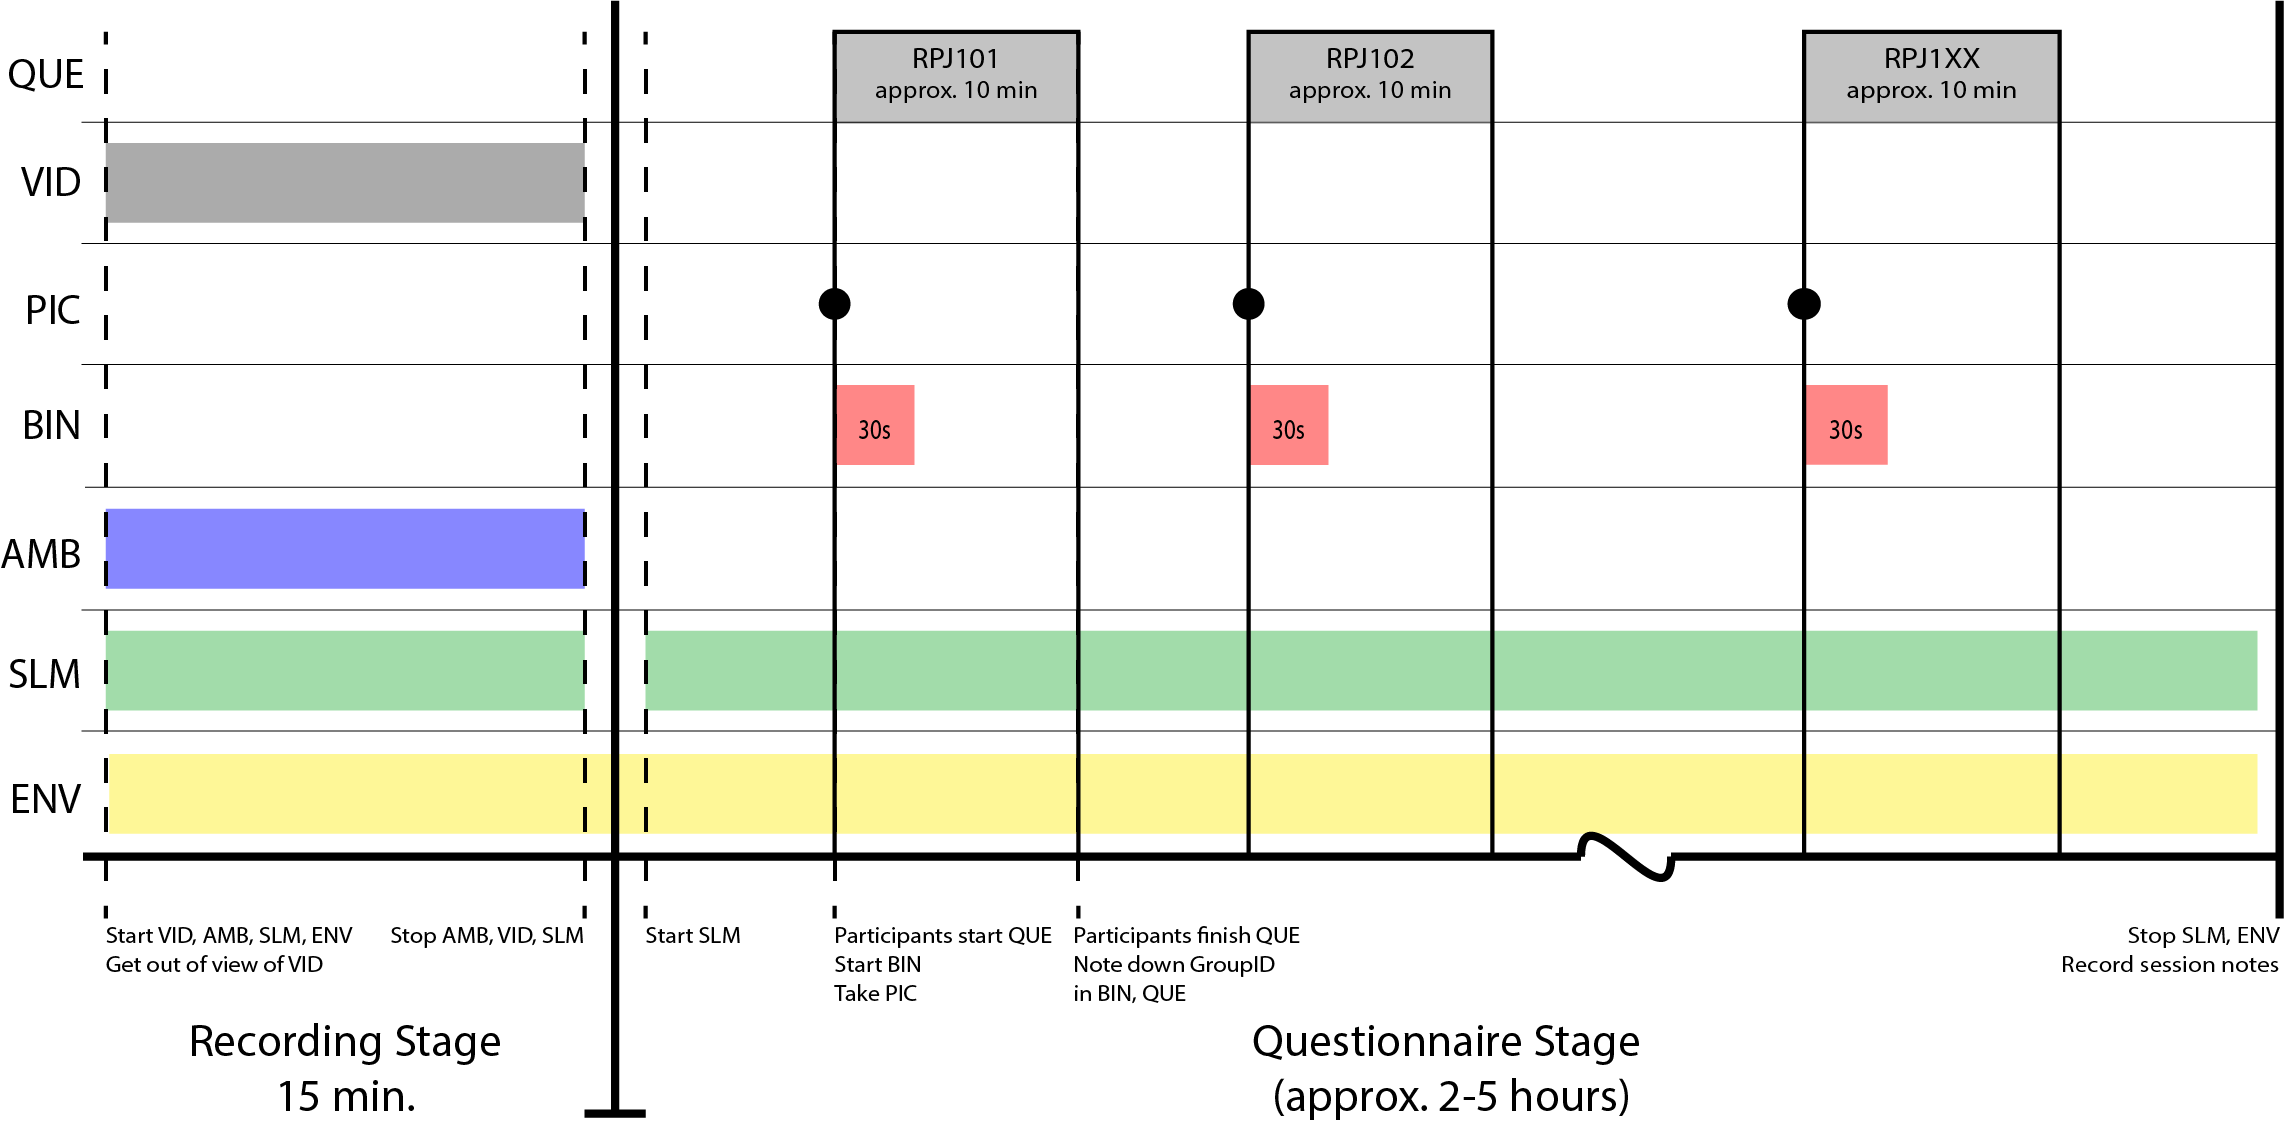
\includegraphics[width=\textwidth]{Figures/Survey-Diagram_V2}
   \caption{Timeline of the on-site soundscape protocol. RegentsParkJapan (RPJ) is used as an example. Abbreviations as defined in Table \ref{tab:factors} -- \gls{que}: Questionnaires; \gls{vid}: 360\degree video; \gls{pic}: Site pictures; \gls{bin}: Binaural Recording; \gls{amb}: Ambisonic recording; \gls{slm}: Sound Level Meter (acoustical factors); \gls{env}: Environmental factors. \label{fig:timeline}}
 \end{figure}

 \paragraph*{Setup \& Calibration} The equipment should be assembled, checked, and calibrated prior to arriving at the measurement location. Calibrate the equipment according to the manufacturer's instructions. All \gls{slm}s should have built-in methods to calibrate using a standard 94 dB 1 kHz tone calibrator. If a similar method is available for the ambisonic microphone, this should be used. If a built-in method is not available, but a calibrator can be fitted to the microphone capsules, then the ambisonic microphone should be calibrated by recording the 1 kHz signal through the system for each microphone capsule after the gain settings have been finalised on site (see below). If it is not possible to calibrate the ambisonic microphone, then the levels recorded will need to be compared to the levels taken simultaneously with the \gls{slm}. This is why it is crucial to have an appropriate quality, calibrated \gls{slm} included within the same setup as the \gls{amb} recordings.

 \begin{figure}[h]
   \centering
   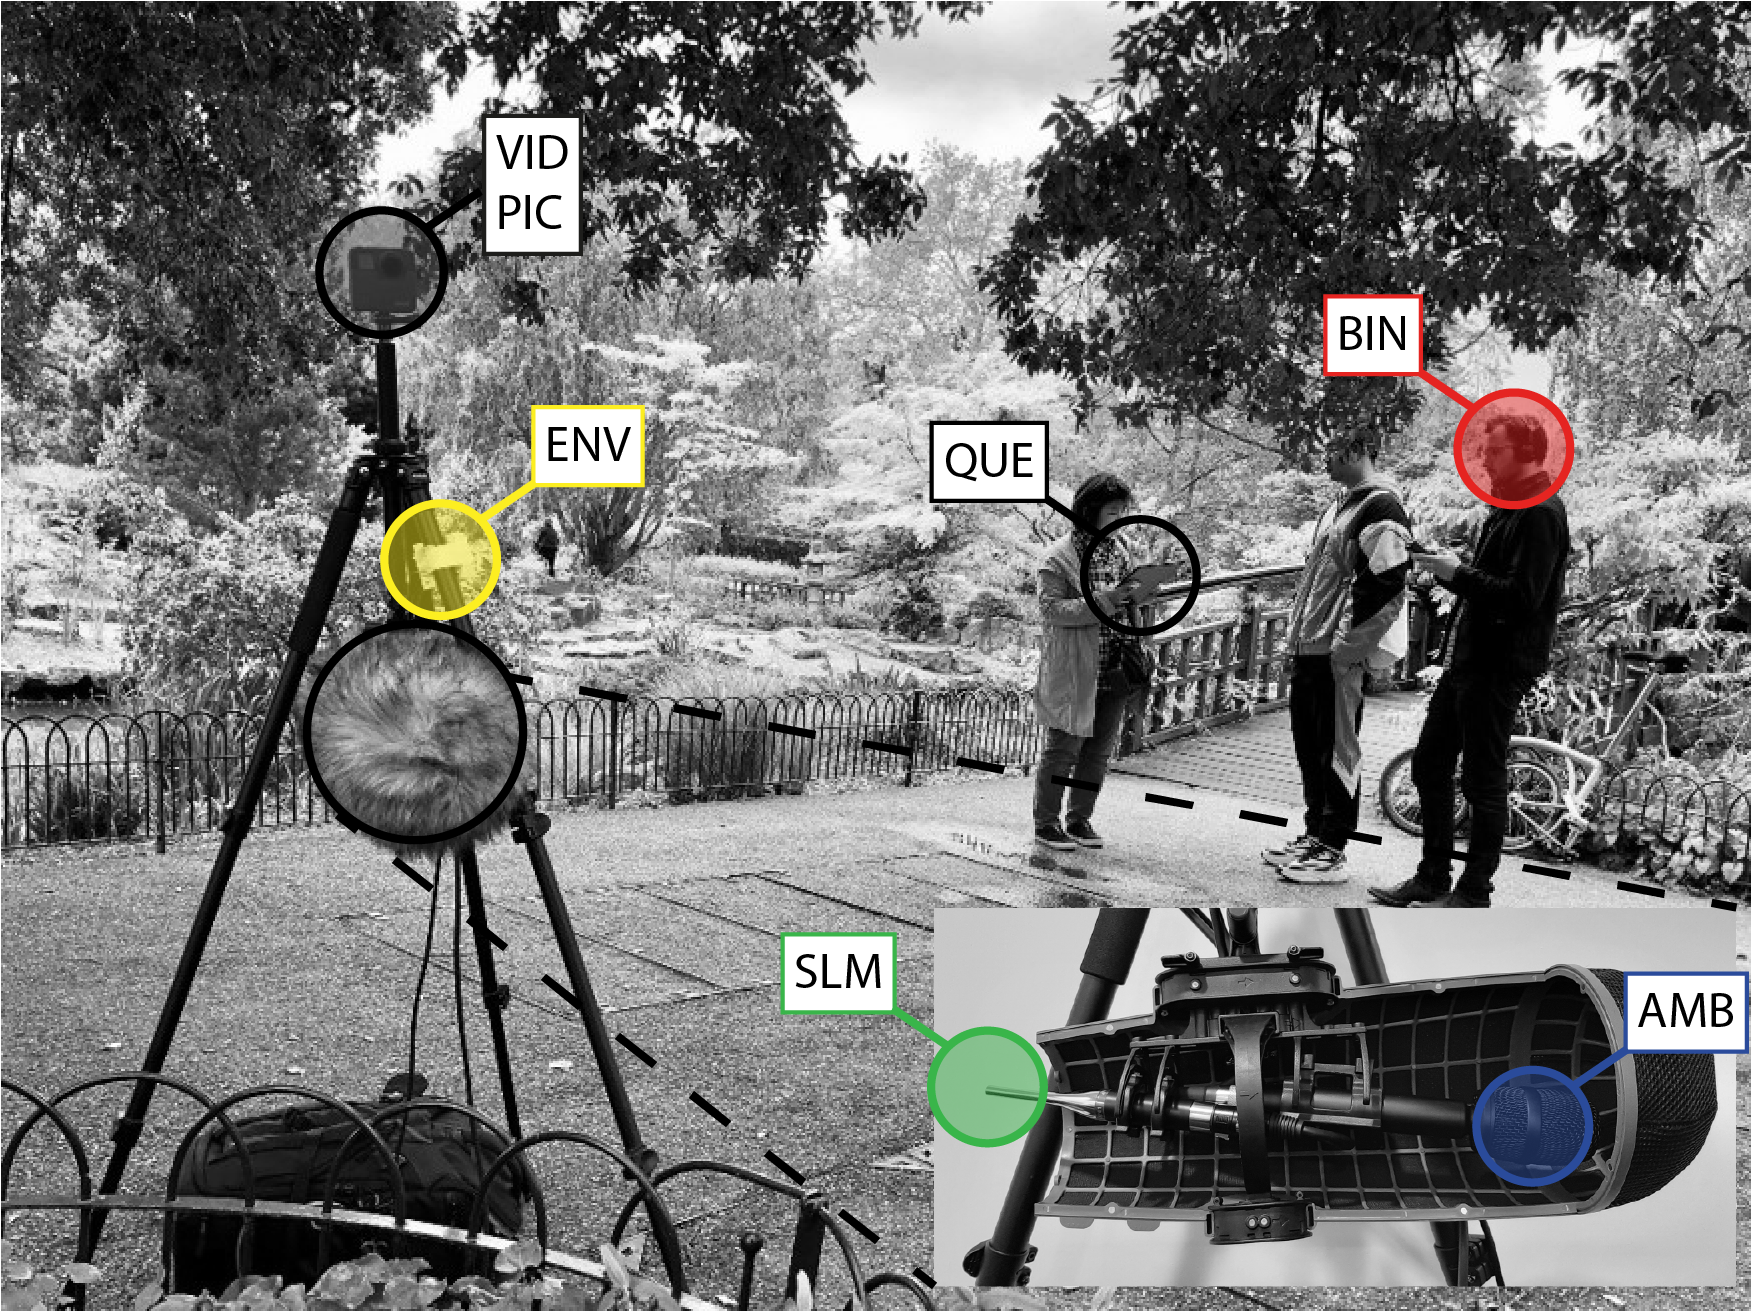
\includegraphics[width=\textwidth]{Figures/RegentsParkSurvey_V2-2}
   \caption{Photo of a full survey carried out in a park in London during the Questionnaire Stage. To the left is the equipment (colour-coded to match \cref{fig:timeline}), with the ambisonic microphone and \gls{slm} microphone in the windscreen, with the 360\degree camera on top of the tripod and to the right are one researcher interacting with the participant while the second researcher conducts the binaural recording. The body of the \gls{slm} and the multi-channel recorder are stored in a bag under the tripod which can contain all of the pieces of equipment for easy transport. \label{fig:survey-pic}}
 \end{figure}

 \subsection{Assembling the Equipment}

   \begin{enumerate}
     \item Set up the equipment by prioritising the position of the 360\degree camera and position the lens at the average eye level 160--180 cm, as shown in \cref{fig:survey-pic}.

           It is advisable to test the setup for video stitching issues and reconfigure if needed (e.g. the equipment will be partially visible in the raw video recording, so you need to test if the chosen setup allows for efficient erasing/hiding/patching of the exposed parts in the post-processing). Companies selling 360\degree cameras usually offer free software for basic editing and previewing. It is advisable to position the camera as the highest item in the set to avoid the need for editing both the sky and the ground.
     \item Carefully position the \gls{amb} microphone so its axes are aligned with the axes of the 360\degree camera; the microphone's front (usually marked by the logo) and the camera's front should be looking in the same direction. Many \gls{amb} microphones allow them to be oriented vertically or horizontally (end-fire), this should be noted and adjusted in the relevant software settings.

           This is essential for informed post-processing. It is advisable to position the capsules of the \gls{amb} microphone and the capsule of the \gls{slm} as near to each other as possible, without introducing scattering effects. It can usually be done within the same windshield unit, but it is not essential to do so and depends on the available clamps and stands.
     \item The gain settings for the four ambisonic audio channels should be set to the same level. In some devices (such as the MixPre10), this can be set by locking the channel gain settings to a single channel. Many devices also offer ambisonic plugins which simplify these settings and automatically link the gain settings -- these should be used where available.
     \item Set the \gls{slm} to log sound levels and simultaneously record .wav audio. The recommended logging settings are given in \cref{tab:equipment}. The \gls{slm} should be mounted and positioned according to standard guidance for environmental noise measurements, like that given in Section 9 of \citet{ISO1996Part1} or Section 5 of \citet{ANSIS129Part1}. Generally, the microphone should be a minimum of 1.2m above the ground and a minimum of 1m from any vertical reflecting surfaces.
     \item Attach the environmental meter(s) to the tripod. Care should be taken when positioning the environmental monitor. Most units will include guidance on their use from the manufacturer -- these should be followed where available. Some general items to keep in mind include not accidentally covering air quality sensor holes, not positioning light sensors in the shade of the other equipment, and not positioning temperature sensors in direct sunlight unless this is how they are intended to be positioned.
   \end{enumerate}

 \subsection{Recording Stage}

   The following section prepares step-by-step instructions for conducting the Recording Stage of the on-site protocol, as shown in \cref{fig:timeline}.

   \begin{enumerate}
     \item Double check all settings and file save locations on the recording equipment.
     \item Adjust gain settings to ensure there is no clipping. Good practice is to listen for what is expected to be the loudest sound event during the recording period (e.g. sirens) and set the gain such that the level is comfortably under clipping during this event.
     \item Start recording on all devices, including the ambisonic microphone, 360\degree camera, \gls{slm}, and environmental meter.
     \item Stand at the front of the camera/ambisonic microphone and clap. The clap can help synchronise the audio with the video, if necessary, and ensuring you are standing in line with the front of the 360\degree video can help with lining up the directionality of the two, if necessary.
     \item Retreat out of view of the camera, blending into the surrounding crowd, or otherwise make sure not to be obvious to someone watching the video.
     \item Record at least 5 min of consistent and representative audio and video. It is recommended to record for 15 min to give the best chance of being able to extract a solid 5 min of useful video and audio.
     \item Stop recording on all devices and ensure all files are saved properly.
   \end{enumerate}

 \subsection{Questionnaire Stage}

   The following section prepares step-by-step instructions for conducting the in-situ questionnaires and their accompanying reference recordings as part of the Questionnaire Stage. Typically these are performed during the same working session as the Recording Stage, using the same set of equipment. The selection of an appropriate location and setup of the equipment should follow the guidance given in \cref{sec:location-selection}, while making sure the location selected is representative of where the respondents will be stopped. Wherever possible, the equipment should be assembled and located so as not to draw the attention of the respondents and particularly to avoid influencing their perception of the space.

   \begin{enumerate}
     \item Double check all settings and file save locations on the recording equipment. If starting this stage immediately after the Recording Stage, make sure to rename or advance the index of the filenames for the \gls{slm} and \gls{env} meters.
     \item Start recording on the \gls{slm} and \gls{env} meter (or leave running from preceding Recording Stage). These will continue running until the end of the Questionnaire Stage.
     \item Gather the tablets and/or paper questionnaires and prepare to approach potential participants.
     \item Approach participants and ask if they would be willing to take part in a research study. If the participants are in a group, they can participate at the same time, but should each fill out a separate questionnaire. When approaching participants, you should identify yourself as a researcher or student researching urban sound. We advise avoiding phrases such as `noise', `noise pollution', `noise disturbance' or other terms which carry a negative connotation. In general, explanations and answers to questions should strive to be as neutral as possible regarding the nature of the soundscape.
     \item Once the participant has consented to participate, hand them the questionnaire or tablet and provide them with basic instructions for answering the questionnaire. Emphasise that they should be responding and assessing the current sound environment, in the current place. Note that this is a common misunderstanding -- many participants assume the questionnaire is focussed on the sound environment at their home, or in the city in general. Where a mix of tablets and paper questionnaires are being used, each group should have at least one participant using a tablet such that start and end times and precise GPS coordinates can be pulled from the accompanying electronic questionnaire. While one researcher is interacting with the participants, the second should arrange the equipment for taking the \gls{bin} recordings and 360\degree photo (\gls{pic}).
     \item Once the participant has started answering the questionnaire, start recording the \gls{bin} audio. If the participants are in a group and all are taking the survey at the same time, only one binaural recording is needed for the whole group. The researcher conducting the recording should strive to keep their head as stationary as possible and to avoid making any extraneous noise.

           Make sure that at least 30s of consistent audio is recorded while the participant is filling in the questionnaire. This should not include talking either from the researcher or the participant. If talking or other intrusive (non-representative) sound occurs, extend the recording period to end up with a solid 30s of good audio. The goal is to capture the sound environment which the participant is exposed to while filling out their questionnaire, but to exclude sounds which the participant is not likely considering as part of their assessment. Most commonly, this would be the researcher talking, or the participant themselves talking. Any other sounds which the participant was `naturally' exposed to should be included.

           When taking the \gls{bin} recording, attempt to orient the head (artificial or researcher wearing a headset) in the same direction as the participants. This is not crucial as it is often impossible to achieve, but it is preferable. Be careful not to move the head during the recording.
     \item Note the GroupID in the metadata for the \gls{bin} recording, or make a manual note of the \gls{bin} recording file name and the GroupID separately.
     \item Take one 360\degree photo (\gls{pic}) with the camera to capture the general setting. This can also be done at regular intervals during the survey session.
     \item When the participant has finished filling in the questionnaire, thank them for their participation and fill in the additional research questions at the end of the questionnaire. These help to both track the data collected and to document the conditions on site. The most important of these are:
           \begin{itemize}
             \item (For paper version) Start and End time. If a Start time was not noted, at minimum, the End Time must be recorded and an average survey duration can be subtracted to estimate the Start Time.
             \item GroupID
             \item SessionID
           \end{itemize}
     \item Repeat steps 4--9 for the remainder of the session, incrementing the GroupID by one with each new group of participants. If there are more than two researchers on site, the additional researchers can stop new groups of participants simultaneously. The researcher operating the \gls{bin} equipment can then shift between the groups once they have finished the 30s recording. This researcher should also have the responsibility of keeping track of the GroupID numbers for each group. Experience has shown this is possible up to about three groups at a time, with four researchers on site.
     \item Once the session is finished, stop the equipment and ensure all files are saved properly.
     \item After each session, make note of the character of the site and the environmental conditions during the survey. This might include, but is not limited to:
           \begin{itemize}
             \item Site typology and intended use (e.g. urban park, transit station, urban square, etc.)
             \item Weather
             \item Crowdedness (i.e. how many people are present in the space)
             \item Dominant sound sources and any key soundmarks
             \item Visual character (e.g. amount of greenness, enclosed vs. open, etc.)
           \end{itemize}
   \end{enumerate}

\section{Lessons from International Data Collection}

 As this protocol has already been implemented by several research groups across four countries, it has undergone a rigorous testing and development process. Throughout this process, adjustments have been made which resulted in the final protocol presented here. However, no process is perfect or applicable in all situations. As such, after consultation with the research groups involved, I have compiled the most common feedback and guidance to keep in mind when implementing this protocol.

 \subsection{Sampling}

   The research groups were instructed to try keeping the structure of respondents well-balanced. This often led to longer times and larger sample sizes required as most comments from five research groups addressed age and type of location as the most influential factors for participant sampling. However, while some reported higher response rates from younger (student) members of the public, others reported higher response rates in case of older highly-educated people. A common observation was that public parks are the locations with the highest response rates, most likely due to a high number of people taking part in activities that allow enough time to take part in a survey. The type of space was also reflected in the sense of privacy. In locations that were more public, people in groups were more likely to take part in the survey, while in the more private locations it was the opposite. Amongst other comments, whether a participant was a tourist or a local also had an influence on the response rate. Tourists seemed more likely to participate in the survey.

   Several groups reported extremely hot and cold weather to negatively affect the response rates. One research group, which conducted the survey also in a residential area, distinguished privacy/ownership of the survey site as a major factor.

 \subsection{Data Collection}

   A group of three researchers seems to be the minimum number needed to conduct the survey, as observed by the partner research groups. A group of nine researchers on site proved to be the most effective number. The time needed to complete the survey varied greatly depending on the location.

   Although the questions are written in a manner that emphasises the focus on the actual acoustic environment perceived at the moment, additional care should be made to ensure a proper understanding of that concept while approaching the participants. Researchers' comments are invaluable here to keep track of the outliers if a researcher feels similar issues or other factors (i.e. wearing headphones) lead to collecting invalid or misleading data.

 \subsection{Equipment}

   Some partners had previous experience in soundscape research, but for all this was the first study that featured surveying a large number of public participants around a single measurement point. All the research groups found it very important to delegate one researcher or technician to care exclusively about the equipment and the quality of the recordings.

   The intention of the recording stage is to record a first-person experience most representative of the location. Therefore, the researchers are instructed to `make themselves invisible' in the recording. However, at some locations, various research groups decided to put out a sign asking members of the public not to touch or come near the measurement point as they experienced passers-by touching the windshield out of curiosity.

   The equipment setup has been designed to be as compact and unobtrusive as possible so as to limit any intrusion on the participant's experience of the space. From our experience, most participants do not end up with the equipment within their field of view during the questionnaire and often do not notice the presence of the stationary equipment. In some locations, this is not possible and participants may comment on its presence; however, over the thousands of surveys collected, only a small number of respondents have commented on the equipment as noticeably impacting their experience.

 \subsection{Translation}

   Regarding the onsite soundscape survey, the translation of the questionnaires (and in particular the perceptual adjectives used for the soundscape appraisal) is a key point to consider when using the protocol in regions where English is not the local language. Indeed, while the ISO/TS 12913-2:2018 document from which the soundscape-related questions of this protocol are derived aims at providing standardised scales, it does not provide official translations in languages other than English. Some perceptual constructs are difficult to render in different languages and people might assign different meanings to them (e.g. \citep{Tarlao2016Comparing,Jeon2018cross,Nagahata2019Examination,AlmagroPastor2019Soundscape}). For this reason, in the soundscape research community, there is a growing interest in testing and validating reliable translation of the ISO soundscape adjectives \citep{Aletta2020Soundscape}, which will hopefully lead to a wide-spread use of this soundscape tool. It is expected that these validated translations could simply be substituted for their English counterparts in this protocol, when they become available.
   
   \subsubsection*{The Soundscape Attributes Translation Project (SATP)}

  % TODO Finish database section
\section{The Database} 
\misc{This section will form the start of the Scientific Data paper.}

The implementation of this protocol within the \gls{ssid} project has resulted in the creation of a large dataset of urban soundscape assessments. The first version of the dataset has been released publicly as The \gls{isd}. This database forms the basis for the majority of the work reported in this thesis.

\draft{Technical description of the database, including organisation}

\draft{Summary including figures of the data}

\draft{The future of the database.}
\chapter{Data Analysis and Modelling}
\label{chap:methods}

 The full experimental protocol developed for this thesis is outlined in \cref{chap:protocol}. The development and presentation of this protocol involved a substantial development and testing phase, and represents a novel advancement in soundscape survey methodology. This chapter therefore presents those methods not associated with the data collection procedure, i.e. the analysis and statistical methods used.

This chapter begins by reviewing the methods presented in \citet{ISO12913Part2} for analysing soundscape assessment data which makes use of the soundscape circumplex, such as that collected with the \gls{ssid} Protocol. Next, a review of machine learning prediction and regression methods is presented. Finally, an in-depth review of the \glsfirst{mlm} method used throughout this thesis is given. 

%%%%%%%%%%%%%%%%%%%%%%%%%%%%%
\section{The current ISO 12913 framework}
\label{sec:current}
Although different methods are proposed for data collection in ISO12913 Part 2 \citep{ISO12913Part2}, in the context of this thesis, I focus on the questionnaire-based soundscape assessment (Method A), because it is underpinned by a theoretical relationship between the items of the questionnaire that compose it. The core of this questionnaire is the 8 perceptual attributes (PA) originally derived in \citet{Axelsson2010principal}, introduced in \cref{sec:paqReview}. In the questionnaire procedure, these PAs are assessed independently of each other, however they are conceptually considered to form a two-dimensional circumplex with \textit{Pleasantness} and \textit{Eventfulness} on the x- and y-axis, respectively, where all regions of the space are equally likely to accommodate a given soundscape assessment \citep{Aletta2016Soundscape}. 

\subsection{Coordinate transformation into the two primary dimensions}
To facilitate the analysis of the PA responses, the Likert scale responses are coded from 1 (Strongly disagree) to 5 (Strongly agree) as ordinal variables. In order to reduce the 8 PA values into a pair of coordinates which can be plotted on the Pleasant-Eventful axes, Part 3 of ISO 12913 \citep{ISO12913Part3} provides a trigonometric transformation, based on the 45\textdegree-relationship between the diagonal axes and the pleasant and eventful axes. This transformation projects the coded values from the individual PAs down onto the primary Pleasantness and Eventfulness dimensions, then adds them together to form a single coordinate pair. In theory, this coordinate pair then encapsulates information from all 8 PA dimensions onto a more easily understandable and analysable two dimensions. The ISO coordinates are thus calculated by:

\begin{equation}
  \begin{split}
    \label{eqn:pleasant}
    ISO Pleasant = [(pleasant - annoying) + \cos 45\degree * (calm - chaotic) \\ + \cos 45\degree * (vibrant - monotonous)] * 1/(4+\sqrt{32)}
  \end{split}
\end{equation}

\begin{equation}
  \begin{split}
    \label{eqn:eventful}
    ISO Eventful = [(eventful - uneventful) + \cos 45\degree * (chaotic - calm) \\ + \cos 45\degree * (vibrant - monotonous)] * 1/(4+\sqrt{32)}
  \end{split}
\end{equation}

where the PAs are arranged around the circumplex as shown in \cref{fig:radar}. The $\cos 45\degree$ term operates to project the diagonal terms down onto the x and y axes, and the $1 \slash (4 + \sqrt{32})$ scales the resulting coordinates to the range (-1, 1). The result of this transformation is demonstrated in \cref{fig:radar}. This treatment of the 8 PAs makes several assumptions and inferences about the relationships between the dimensions. As stated in the standard \citep[p. 5]{ISO12913Part3}:

\begin{quote}
  According to the two-dimensional model, vibrant soundscapes are both pleasant and eventful, chaotic soundscapes are both eventful and unpleasant, monotonous soundscapes are both unpleasant and uneventful, and finally calm soundscapes are both uneventful and pleasant.
\end{quote}

\begin{figure}
  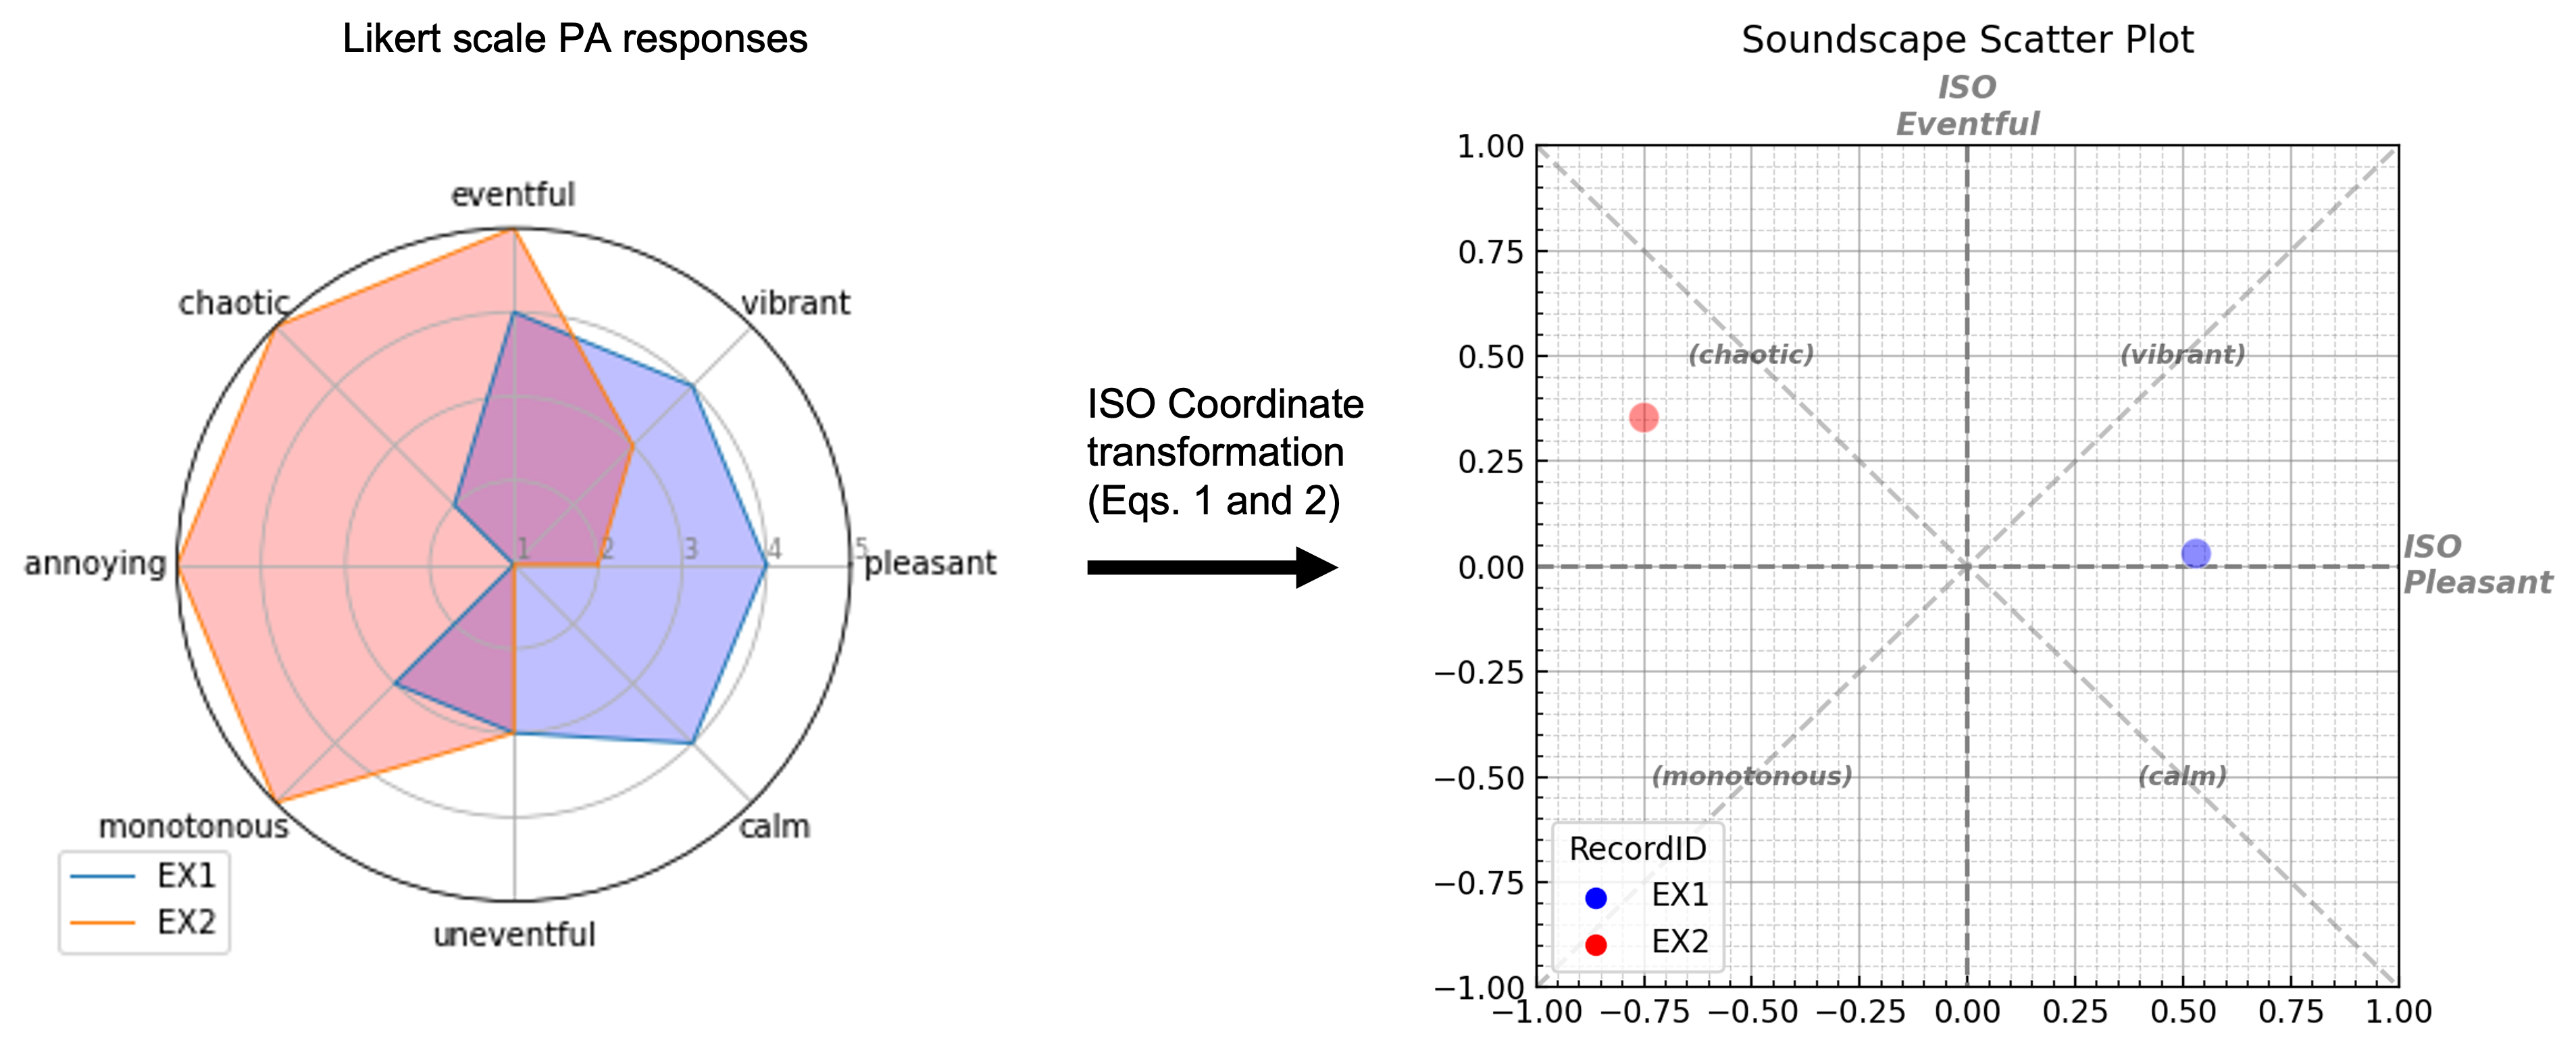
\includegraphics[width=\textwidth]{Figures/jasa-el_Figure1.png}
  \caption{Example of representations of two soundscape assessments. Left: Radar plot of two example perceptual attribute (PA) ratings on the Likert scales (1 to 5). Right: Scatter plot of the same assessments on the soundscape circumplex, transformed according to ISO 12913 Part 3.
    \label{fig:radar}
  }
\end{figure}

\subsection{Interpreting the soundscape circumplex}
The circumplex model of soundscape, as originally defined by \citet{Axelsson2010principal}, is commonly understood to be a two-dimensional space (its main orthogonal components being annoying-pleasant and uneventful-eventful) where all regions of the space are equally likely to accommodate a given soundscape assessment \citep{Aletta2016Soundscape}. For instance, in theory, an extremely vibrant soundscape (e.g., with a score of 1) should be as likely to occur as an extremely annoying one, as well as one neutral on all dimensions (e.g., with a score of 0). However, a recent work by \citet{Lionello2021Introducing} incidentally highlighted a possible issue with the process for representing soundscape assessments with the current ISO protocols. More specifically, when considering big numbers, soundscape assessments seem to have a bivariate normal distribution around the origin of the circumplex model. This would imply that not the whole space of the model is equally accessible to any given soundscape\footnote{\cref{app:CircCritique} offers a more in-depth critical critique and discussion of the specific consequences of this projection method in more detail than is appropriate to include here.}. Studies in the field show that data collection campaigns rarely return extreme values for soundscape dimensions \citep{Mancini2021Soundwalk} and so far the general interpretation has been that some soundscapes (e.g., extremely monotonous) may simply be difficult to find and detect with people in urban contexts \citep{Sun2019Classification}.

\subsection{Usefulness for predictive modelling}
This trigonometric projection method enables us to transform the 8 Likert scale PAQ values into a pair of coordinate values. This transformation has a few beneficial effects for applying standard modelling techniques to soundscape data. First, it simplifies and reduces the target problem; rather than needing to model eight separate responses, we are now focussed on only two. Second, it transforms the data from ordinal responses on a 1 to 5 scale into continuous values between -1 and +1. While it is clearly possible to model ordinal outputs through classification, the methods are often less familiar and more complicated than dealing with a more standard regression problem. For those outside of machine learning (i.e. designers, engineers, etc.) regression methods, especially linear regression, are already familiar and interpretable while methods of classification and ordinal modelling are typically less familiar. By applying the \gls{iso} projection to each individual's soundscape assessment, we generate a vector of output values which can be matched up to physical data measured for each individual. This creates the sort of input-output pair vector necessary for supervised regression learning.

\section{Machine learning and regression techniques}
Machine learning approaches are typically divided into three broad categories: supervised, unsupervised, and reinforcement learning. In supervised learning, the training data consists of input-output pairs and trains a model which can map from the inputs to the outputs. In unsupervised learning, no corresponding output data is available to the training model, thus it learns patterns in the input without feedback. Reinforcement learning does not necessarily begin with training data, instead the learning agent is given a series of reinforcements in the form of rewards and punishments \citep{StuartRussell2021}. Reinforcement learning will not be used in this thesis. Unsupervised learning has been applied to a limited degree to the acoustic data collected in several sound environments which will be expanded upon in \cref{ch:lockdown}. 

The majority of this thesis is therefore focussed on creating a supervised learning model wherein the input data are the result of measurements and the output data are the perceptual assessments of the soundscapes. In the context of this thesis, there are two primary types of supervised machine learning models - regression and classification. Regression is applied when the output is a continuous number (e.g. temperature) whereas classification is used when the output is a discrete set of values. 



\subsection{Multi-level linear regression}

Multi-level regression modelling is a technique commonly used in fields such as psychology \citep{Quene2004multi,VolpertEsmond2021Using}, for applied prediction models \citep{Gelman2006Multilevel,Frees2006Multilevel}, and for a small number of previous soundscape studies \citep{Aumond2017Modeling}. \glspl{mlm} are particularly useful when data is organised at one or more levels or groups. As noted in \cref{tab:metadata}, the \gls{isd} forms a hierarchical structure with several groups nested within each other: Questionnaires within GroupIDs within SessionIDs within Locations, making a \gls{mlm} especially well-suited. The inherent grouped structure of the \gls{isd} necessitates a modelling and analysis approach which considers the differing relationships between the objective acoustic features and the soundscape's perceived affective quality ratings across the various locations and contexts. \glsplural{mlm} are also well-suited for engineering and design contexts as they are transparent, understandable, and conceptually familiar to most engineers. The concept behind \glspl{mlm} can be built up starting from simple linear regression \citep{DataAnalysisUsingGelman}, as given by:

\begin{equation}
  y_i = \alpha + \beta x_i + \epsilon
\end{equation}

For a classical multiple linear regression, we expand the $k$ coefficients out as so:

\begin{equation}
  \label{eqn:classicRegressModel}
  y_i = \alpha + \beta_1 x_{i1} + \ldots + \beta_k x_{ik} + \epsilon_i
\end{equation}

where:

\begin{itemize}
  \item \emph{i} indexes each unit, the smallest items of measurement. This is often a measurement per individual within a group or, in the \gls{isd} this can be for each recording.
  \item $y_i = (y_1, \ldots, y_n)$ the modelled outcome for each unit \emph{i};
  \item $k = 1, \dots, K$ denotes each of the multiple predictors;
  \item $\beta_k$ is the slope coefficient for the \emph{k\textsuperscript{th}} predictor;
\end{itemize}

Their primary feature of an \gls{mlm} is the ability to have coefficients and intercepts which are allowed to vary depending on the group \citep{DataAnalysisUsingGelman}. This can take three forms, which are illustrated in \cref{fig:GelmanMLM}:

\begin{enumerate}
  \item Varying intercepts
  \item Varying slopes
  \item Varying intercept and varying slopes
\end{enumerate}

\begin{figure}[h]
  \centering
  \begin{subfigure}[b]{.3\textwidth}
    \centering
    \caption{Varying intercepts}
    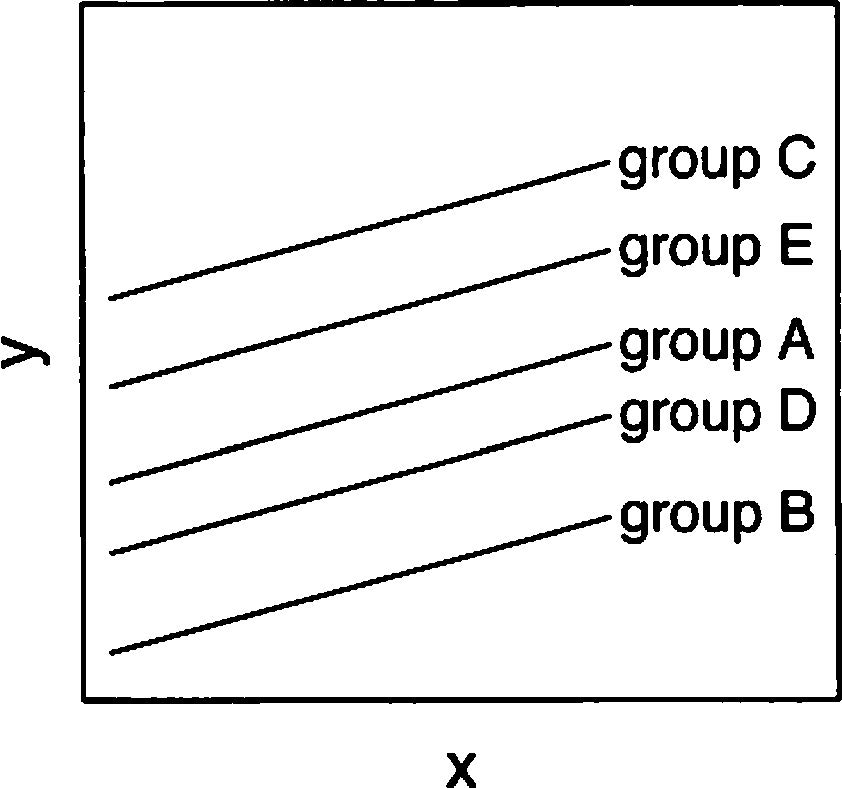
\includegraphics[width=\textwidth]{Figures/GelmanMLMa.jpg}    
  \end{subfigure}
\hfill
  \begin{subfigure}[b]{.3\textwidth}
    \centering
    \caption{Varying slopes}
    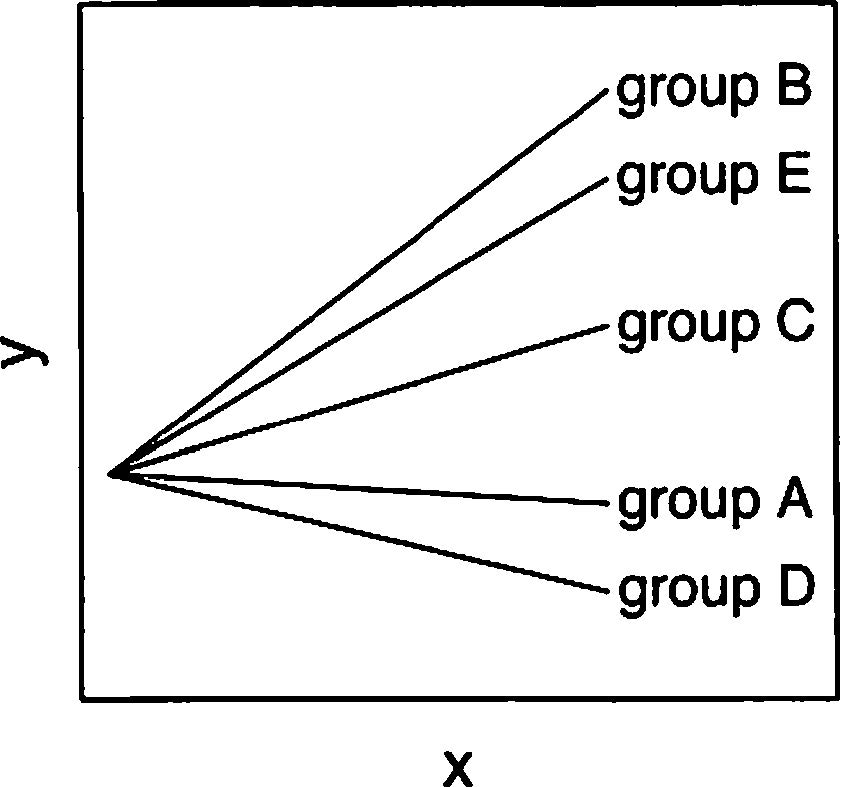
\includegraphics[width=\textwidth]{Figures/GelmanMLMb.jpg}    
  \end{subfigure}
\hfill
  \begin{subfigure}[b]{.3\textwidth}
    \centering
    \caption{Varying intercepts and slopes}
    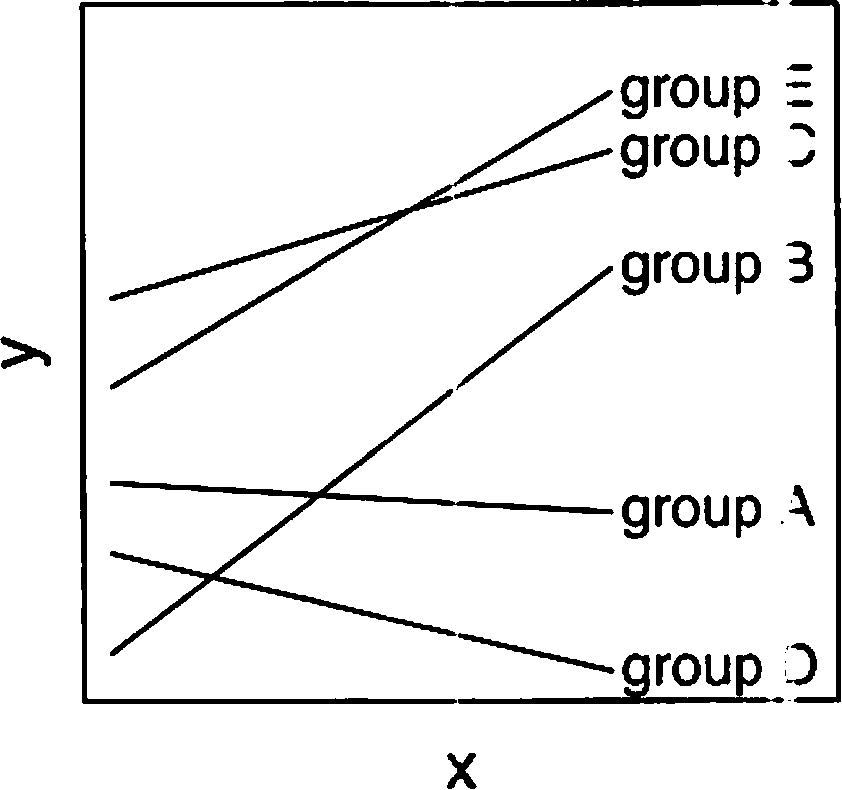
\includegraphics[width=\textwidth]{Figures/GelmanMLMc.jpg}    
  \end{subfigure}
  \hfill

  \caption{Linear regression model with with (a) varying intercepts ($y=\alpha_j + \beta x$), (b) varying slopes ($y=\alpha + \beta_j x$), (c) both ($y=\alpha_j + \beta_j x$). The varying intercepts correspond to group indicators as regression predictors, and the varying slopes represent interactions between \emph{x} and the group indicators. Reproduced with permission from \citet[Fig. 11.1]{DataAnalysisUsingGelman}. \label{fig:GelmanMLM}}
\end{figure}

In a varying intercept structure, the intercept for each input feature is allowed to vary according to the second level. This structure assumes that the linear relationship between each input feature and the output is consistent across the second level groups, but that the zero point (the intercept) is different. This is expressed mathematically \citep{DataAnalysisUsingGelman} as:

\begin{equation}
  y_i = \alpha_{j[i]} + \beta x + \epsilon{i}
\end{equation}

where groups are indexed by $j = 1, \ldots, J$, and \emph{j[i]} is the \emph{i\textsuperscript{th}} individual \emph{i} in group \emph{j}. This results in a vector of length \emph{J} containing one intercept result per group.

In the context of auditory perception studies, this is most appropriate for repeated measures experimental designs (as will be demonstrated in \cref{ch:mlmann}). One type of repeated measures studies is one in which all participants experience all levels of the independent variables and provide some response in terms of the output variable. In other words, each participant constitutes a group in the model and they respond to all of the input variables \citep{Kristjansson2007Multilevel}. In this case, the \gls{mlm} framework is used to account for starting differences between respondents; populations are expected to demonstrate similar behaviours in response to a given stimulus, but may have differing initial starting points, i.e. different intercepts for each analysed feature. The \gls{mlm} framework using a varying intercept for each participant allows this initial difference among individuals to be accounted for while also highlighting the overall relationship between e.g. acoustic features and annoyance ratings for a given sound. 

Varying slope structures take the opposite assumption; each level shares the same intercept, while the coefficients for each feature are allowed to vary depending on the group. This assumes that different groups will have a different relationship between the input features and the output, but that these relationships may begin at a different threshold. This structure appears to be less commonly used than varying intercept models. This can be mathematically described as \citep{DataAnalysisUsingGelman}:

\begin{equation}
  %TODO: insert random slope equation from Gelman 2006
  y_i = \alpha + \beta_{j[i]}x_i + \epsilon_i
\end{equation}

where $\beta_{j[i]}$ is the slope coefficient for individual \emph{i} in group \emph{j}. 

With multiple predictors, we write:

\begin{equation}
  y_i = X_i B + \epsilon_i
\end{equation}

where B is a matrix of slope coefficients of size $J\times K$ with one coefficient for each predictor (\emph{k}) for each group (\emph{j}):

\[
  B_{J\times K} =
  \left[ {\begin{array}{cccc}
    \beta_{11} & \beta_{12} & \cdots & \beta_{1K}\\
    \beta_{21} & \beta_{22} & \cdots & \beta_{2K}\\
    \vdots & \vdots & \ddots & \vdots\\
    \beta_{J1} & \beta_{J2} & \cdots & \beta_{JK}\\
  \end{array} } \right]
\]

Finally, a varying-slope, varying-intercept model allows both the slope and intercept of the coefficients to vary for each group in the second level:

\begin{equation}
  y_i = \alpha_{j[i]} + \beta_{j[i]}x_i + \epsilon_i
\end{equation}

\paragraph*{Wilkinson-Rogers notation}
The analysis package used for constructing these models is \texttt{lme4} \citep{Bates2015Fitting} in the R statistical language \citep{RCT2018R}. This package makes use of a style of writing \glsplural{mlm} called Wilkinson-Rogers notation \citep{Wilkinson1973Symbolic}. Wilkinson-Rogers notation provides a way to specify \glsplural{mlm} without the need to specify coefficient values in a straightforward and easily readable way. For these models, the important operators to be familiar with are: $\sim$ indicates that a model regresses on the dependent variable; $+$ sums the model terms;$\cdot$ indicates interaction terms; \texttt{(var|grp)} specifies a grouping variable or random effects term for an \gls{mlm}\footnote{It appears this notation was an extension of Wilkinson-Rogers introduced into the \texttt{nlme} R package by \citet{Pinheiro1997Graphical}.}. \cref{tab:wilkRog} shows some example models written in Wilkinson-Rogers notation:

\begin{table}[h]
\centering
\caption{Mathematical and Wilkinson-Rogers notation for several example models to demonstrate how to translate from one to the other. \texttt{var} is used to denote the independent variables to demonstrate that the variable name (e.g. \emph{loudness}) can be used directly in the notation. \label{tab:wilkRog}}
\resizebox{\linewidth}{!}{%
\begin{tabular}{lll} 
\toprule
\textbf{Description}                                                      & \textbf{Model}                                                                        & \textbf{Wilkinson-Rogers Notation}   \\
Two predictors                                                            & $y_i = \beta_0 + \beta_1 x_{i1} + \beta_2 x_{i2} + \epsilon_i$                        & \texttt{y $\sim$ var1 + var2}                 \\
\begin{tabular}[c]{@{}l@{}}Two predictors \\and no intercept\end{tabular} & $y_i = \beta_1 x_{i1} + \beta_2 x_{i2} + \epsilon_i$                                  & \texttt{y $\sim$ var1 + var2 - 1}             \\
\begin{tabular}[c]{@{}l@{}}Two predictors \\with interaction\end{tabular} & $y_i = \beta_0 + \beta_1 x_{i1} + \beta_2 x_{i2} + \beta_3 x_{i1}x_{i2} + \epsilon_i$ & \texttt{y $\sim$ var1 $\cdot$ var2}           \\
Varying intercept                                                          & $y_i = \alpha_{j[i]} + \beta_{x_i} + \epsilon_i$                                      & \texttt{y $\sim$ var1 + (1\textbar{}grp)}     \\
Varying slope                                                              & $y_i = \alpha + \beta_{j[i]x_i} + \epsilon_i$                                         & \texttt{y $\sim$ 1 + (var1\textbar{}grp)}     \\
\begin{tabular}[c]{@{}l@{}}Varying slope \\Varying intercept\end{tabular}   & $y_i = \alpha_{j[i]} + \beta_{j[i]x_i} + \epsilon_i$                                  & \texttt{y $\sim$ var1 + (var1\textbar{}grp)}  \\
\bottomrule
\end{tabular}
}
\end{table}

The structure inherent within the \gls{isd} means that this approach is particularly appropriate. In order to further demonstrate the structure and use of an \gls{mlm}, I'll further describe it in terms of the \gls{isd} data, where the most obvious second level for this \gls{mlm} is the location (a categorical variable defined by the LocationID). To demonstrate this, we'll specify a simple varying-intercept varying-slope \gls{mlm} which has the loudness (\gls{n5}) and sharpness (\gls{s}) as the two input variables, the recordings (taken per group in the \gls{isd} and indexed by the GroupID) make up the units at level 1, and the LocationID is level 2. 

\begin{equation}
  \label{eqn:basicISDMLM}
  \texttt{ISOpl $\sim$ loudness + sharpness + (loudness + sharpness | LocationID)}
\end{equation}

which would also be written as:

\begin{equation}
  ISOPl_i = \alpha_{j[i]} + \beta_{j[i]}N_{5_i} + \beta_{j[i]}S_i + \epsilon_i
\end{equation}

where $\alpha_{j[i]}$ is the mean \gls{isopl} score for LocationID \emph{j} where recording \emph{i} was taken and $\beta_{j[i]}N_5$ and $\beta_{j[i]}S$ are the loudness and sharpness slope coefficients for location \emph{j}. 

\paragraph*{Mixed effects: fixed and random effects} In some applications and fields, it is more common to refer to a \gls{mlm} as a \glsfirst{lmer}, however the two are simply different ways of speaking about the same mathematical concept \citep{Pinheiro2000Linear,DataAnalysisUsingGelman}. Although I typically refer to \glsplural{mlm}, I sometimes find it helpful to use the random-effects/fixed-effects terminology and \cref{ch:whostudy} primarily refers to the model as an \gls{lmer} since that work was targeted at a psychology audience, where mixed-effects is the more common term. In a varying-intercept varying-slope model, where certain features can be specified only at the unit level and others vary at the group level, the features at the unit level are considered \emph{fixed}: i.e. the relationship between independent and dependent variable remains fixed across all groups. In an \gls{lmer} the second level of effects are then termed the \emph{random effects}. This is useful -- particularly in a varying-intercept model -- where the effects in this second level are somewhat unexplainable. Consider a repeated measure study using a varying-intercept model: the grouping factor is the participant who has been exposed to multiple inputs. The second level operates to account for that participants consistent difference from the other participants, but that difference can be considered to be random for each participant, hence it is a \emph{random} effect when the goal is to elucidate the effects which are consistently seen across the sample. However, this use of the word random to refer to the second-level effects is not always useful, as highlighted by \citet[pg. 2]{DataAnalysisUsingGelman}. When we expect the grouping factor to have some explainable impact on the relationship between the independent and dependent variables (e.g. the context of the location has a complex, but non-random effect on the soundscape perception), then it is not appropriate to refer to it as `random'. 

In all, this concept helps to highlight the specific benefit of a \gls{mlm} approach. Conceptually, it would be possible to achieve a similar goal by treating the grouped data as `fully un-pooled' and to fit a separate linear regression model for each group. In the case of \cref{eqn:basicISDMLM}, we would treat the data from each location as a separate dataset and train a model on them each independently. This would reveal, within each location, the relationship between the loudness and sharpness of a sound and its perceived pleasantness. However, it would ignore the fact that there is a general, \emph{fixed}, relationship between loudness and pleasantness, regardless of the effects of the location.Alternatively, we could treat the data as `fully-pooled', creating a linear model with the form given in \cref{eqn:classicRegressModel} and only considers the fixed relationship across the entire dataset. A \gls{mlm}, which treats the data as `partially-pooled', and includes effects which are both fixed and can vary according to the location, enables us to investigate both the degree to which loudness generally impacts on pleasantness \emph{and} how this relationship changes according to the context of the location. 

\subsubsection{Structural equation models}

\gls{sem} is a statistical approach to testing hypotheses about relationships between variables and latent features which has been used by several studies in soundscape \citep{Tarlao2020Investigating,Hong2015Influence,Torresin2022Indoor}. \gls{sem} is a flexible approach in that it can include one or more independent or dependent variables and the variables can be continuous or discrete, factors or measured. As a collection of statistical methods, \gls{sem} is focussed on causal inference and is fundamentally built on a combination of path diagrams and regression modelling techniques \citep{Ullman2012Structural}. Most frequently in an \gls{sem}, the researcher constructs a path diagram (often called \glsplural{dag}) which expresses the hypothesised relationships between the variables of interest. These path diagrams can be quite complex, including covariance relationships, latent variables, residuals, and distinctions between factors and measured variables. The model is then fit to the data through a selected estimation method (most typically Maximum likelihood (ML) as in regression modelling) and evaluated. The model may then be further reduced or modified if necessary. \gls{sem} also allows for multilevel modelling where separate models are developed for different levels of a nested hierarchy. This is conceptually equivalent to the \gls{mlm} or \gls{lmer} discussed throughout this thesis. Several studies in the soundscape literature have made use of \gls{sem}. However, given the focus on predictive (rather than inferential) models in this thesis, \gls{mlm} is a much more suitable approach.


 \subsection{Feature selection}
 \label{sec:featureSelection}
In general, throughout this thesis, two models are built separately: one for predicting \gls{isopl} and one for predicting \gls{isoev}. A separate backwards-step feature selection was performed for each of the outcome models in order to identify the minimal feature set to be used for predicting each outcome. In this feature selection process, an initial model containing all of the candidate features was fit. Each feature was then removed from the model one at a time, then the best-performing model is selected and the procedure continues step-wise until no improvement is seen by removing more features. This process is carried out first on the location-level features (including the potential to remove all features including LocationID, resulting in a `flat' or standard multivariate linear regression model), then on the individual-level features.  To check for multicollinearity among the selected features, the \gls{vif} was calculated and a threshold of $\gls{vif} < 5$ was set. Any features which remained after the backwards step-wise selection and which exceeded this threshold were investigated and removed if they were highly collinear with the other features.

The model fitting and feature selection was performed using the \texttt{step} function from \texttt{lmerTest} (v3.1.3) \citep{Kuznetsova2017lmerTest} in R statistical software (v.4.0.3) \citep{RCT2018R}. The summaries and plots were created using the \texttt{sjPlot} package (v.2.8.6) \citep{Luedecke2021sjPlot} and \texttt{seaborn} (v.0.11.1) \citep{Waskom2021seaborn}.

\section{Conclusion}
This chapter presents the overarching analysis methods used throughout this research. Although a range of modelling methods have been used in soundscape studies, the multi-level modelling strategy described here was selected due to the inherent multi-level nature of the \gls{isd} data, its relative simplicity and conceptual familiarity, and as a fully transparent and interpretable regression method. Throughout the following chapters, additional modelling, psychoacoustic analysis, scoring, and feature selection information will be presented where it differs from that presented here or to provide context specific to the study being discussed.

  %  \subsubsection{Mutual Information}
  %  \draft{It appears that mutual information is related to the Bayes formula. I still need to read more into this, but it appears based on relative and overlapping probability distributions between the variables in question.}
  %  \paragraph*{From scholarpedia:}
  %  % http://www.scholarpedia.org/article/Mutual_information
  %  \draft{Based on entropy, where the uncertainty about a variable can be expressed as "the number of yes/no questions it takes to guess a random variable, given knowledge of the underlying distribution and taking the optimal question-asking strategy". "The mutual information is therefore the \emph{reduction} in uncertainty about variable $X$, or the expected reduction in the number of yes/no questions needed to guess $X$ after observing $Y$.". }

  %  \draft{"Mutual Information is just one way among many of measuring how related two variables are. However, it is a measure ideally suited for analyzing communication channels. Abstractly, a communication channel can be visualized as a transmission medium which receives an input $x$ and produces an output $y$. If the channel is \emph{noiseless}, the output will be equal to the input. However, in general, the transmission medium is noisy and an input $x$ is converted to an output $y$ with probability $P_{Y|X}(y|x)$. }
  %  \misc{This seems very useful for my conception of sound perception / auditory processing, where the perception system is a noisy communication channel.}

  %  \subsubsection{Conditional Mutual Information}
  %  The Mutual Information between two variables, given another variable as a control.

%  \subsection{Clustering Analysis}
%    \paragraph{K-means}
%    \paragraph{nbclust}


\part{A novel application of predictive soundscape modelling}
\chapter{Investigating Urban Soundscapes of the COVID-19 Lockdown: A predictive soundscape modelling approach}
\label{ch:lockdown}

This paper is part of a special issue on COVID-19 Pandemic Acoustic Effects.

\draft{Will update to match published version, but essentially won't need to change.}

\section*{Abstract}
 The unprecedented lockdowns due to COVID-19 in spring 2020 triggered changes in human activities in public spaces. A predictive modelling approach was developed to characterise the resulting change in the perception of the sound environment when people could not be surveyed. Building on a database of soundscape questionnaires ($N = 1,136$) and binaural recordings ($N = 687$) collected in 13 locations across London and Venice during 2019, new recordings ($N = 571$) were made in the same locations during the 2020 lockdowns. Using these 30-second-long recordings, linear multi-level models were developed to predict the soundscape pleasantness ($R^2=0.85$) and eventfulness ($R^2=0.715$) during the lockdown and compare the changes for each location. The performance was above average for comparable models. An online listening study also investigated the change in sound sources within the spaces. Results indicate:

 \begin{enumerate}
   \item human sounds were less dominant and natural sounds more dominant across all locations;
   \item contextual information is important for predicting pleasantness but not for eventfulness;
   \item in general, perception shifted towards less eventful soundscapes and to more pleasant soundscapes for previously traffic-dominated locations, but not for human- and natural-dominated locations.
 \end{enumerate}

 This study demonstrates the usefulness of predictive modelling and the importance of considering contextual information when discussing the impact of sound level reductions on the soundscape.

 \section{Introduction}
\label{sec:intro}

\subsection{Review of the impacts of COVID-19}
 \label{sec:covidReview}
 The global emergency cause by the \gls{covid19} in early 2020 required national lockdown measures across the world, primarily targeting human activity. In the United Kingdom, construction and transport were allowed to continue, but a decrease in activity was observed \citep{Hadjidemetriou2020impact}. In other countries, such as Italy, the restrictions were more severe and even included limiting people's movement to a certain radius from their place of residence \citep{Ren2020Pandemic}. The explorations in environmental acoustics of lockdown conditions across the world have revealed various degrees of impact on the acoustic environment, with researchers reporting reductions in noise levels affecting the population at the scale of urban agglomerations such as the Ruhr Area in Germany \citep{Hornberg2021Impact} and conurbations in the south of France \citep{Munoz2020Lockdown}. Impacts have also been reported at a scale of a multimillion city such as Madrid \citep{Asensio2020Changes} or Barcelona \citep{BonetSola2021Soundscape} as well as at a more local, city-centre or even public space-scale in cities such as Stockholm \citep{Rumpler2021Noise}, London \citep{Aletta2020Assessing}, Girona \citep{AlsinaPages2021Changes}, or Granada \citep{VidaManzano2021sound}. In general, these studies have demonstrated a decrease in urban noise levels and indicated a difference in the amount of decrease depending on the type of space investigated (e.g. parks, urban squares, etc.) and the type of human activity characteristic for the space, with higher reductions in places typically associated with human sounds and activities such as shopping and tourism.

 Those studies were mostly focussed around the \gls{laeq}, as well as a standardization approach to reporting subsequent changes in soundscape proposed by \citet{Asensio2020Taxonomy}. They were not able to reveal the perceptual impact of such conditions in public spaces as well because of: 1) the lack of subjective data for the exact or comparable locations in previous years; and 2) the lack of participants present in public spaces during the lockdown, hence the ability to collect soundscape data in situ. Attempts have been made to bridge this gap by using social networks to source subjective data, but this resulted in a focus on indoor conditions following the shift in the citizens' behaviour, i.e. spending more time indoors \citep{Bartalucci2021survey,Lee2021Attitudes}. \citet{GarridoCumbrera2021Perceptions} relied on an online survey deployed in England, Ireland, and Spain to explore the perceived change in natural environments in particular. They observed a consistent increase in the perceived presence of natural sounds across all major cities and rural areas respectively in these three countries. A very similar trend was observed in Argentina, also based on an online questionnaire without a listening task \citep{Maggi2021Perception}. 
 
 \citet{Munoz2020Lockdown} combined noise measurements with an online questionnaire deployed to residents, some of which were residing in the areas covered by the noise monitoring network available. The participants were asked to recall how their lockdown area sounded before and during the first lockdown in 2020 and to describe the perceived change. They observed a consistent reduction in levels, followed by the perceived reduction of transport sounds (air and road) and an increase of natural sounds, while the resulting environment was described as pleasant, calm, and peaceful. By combining field recordings and focus groups, \citet{Sakagami2020How} and \citet{Lenzi2021Soundscape} observed changes in the sound source composition and the affective quality of soundscape in a residential area in Kobe, Japan and a public space in Getxa, Spain, respectively, during the different stages of the lockdown period. Following the easing of lockdown measures, a decrease in animal and traffic sounds was observed in Kobe, while an increase in eventfulness, loudness, and presence of human sound sources, followed by a decrease in pleasantness, was shown in Getxa.

 \subsubsection{The impacts of the lockdown in London}
 \citet{Aletta2020Assessing} explored the impacts of the \gls{covid19} lockdowns on the acoustic environment in London in particular, through many short-term (30s) binaural recordings and presented an important early analysis of the changes in acoustic features during the lockdown. The data from this study form the basis for the modelling presented in this chapter; the results and analysis of \citep{Aletta2020Assessing} were performed by the author of this thesis and are reviewed in depth. 

 %NOTE: The paras and figures here are taken directly from Aletta2020 and Tong 2021, but represent the work I did on the paper. May need to check if this is fine to present it this way.
 The lockdown measures implemented in the UK to contain the spread of the SARS-CoV-2 virus were not particularly strict if compared with other countries. In general, lockdown measures involved "staying at home" recommendations, social distancing, stopping non-essential commercial activities, banning public gatherings, limiting traffic mobility and alike. Specifically, the UK Government passed the Health Protection (Coronavirus, Restrictions) (England) Regulations 2020, which were put into place at 1:00 pm on \nth{26} March 2020 \cit{Public Health England, 2020}. Under these restrictions, the public were only allowed to leave their homes once per day for essential activities and exercise. All officers and shops selling non-essential goods were told to close, gatherings of more than two people in public were banned, and individuals were advised to only interact with members of their own household. These restrictions were set to be reviewed by the Secretary of State at least once every 21 days and would continue indefinitely until they were no longer necessary to prevent the spread of infection in England. In practice the lockdown continued through the spring of 2020 and was first partially eased on the \nth{1} of June, with school children in England returning to school, but the broader lockdown continued throughout the summer \citep{Tong2021Increases}.

 Taking advantage of short-term acoustic measurements carried out in 2019 which formed the \gls{isd}, before the implementation of the lockdown measures related to \gls{covid19}, a number of urban locations were selected in London where data were available and measurements were performed again according to the same protocols to assess the extent of sound level variation achieved at each site. 

 \paragraph*{Data analysis}
 From the binaural recording datasets (both the 2019 and 2020 series), the following acoustic parameters were computed for the left and right channels and the arithmetic average was presented: \gls{laeq}, \gls{la10}, \gls{la90}. There is still no clear consensus on how to merge binaural psychoacoustic readings into single values; in the case presented in \citet{Aletta2020Assessing} an arithmetic average level was deemed to be acceptable as the interaural level difference was typically very small (less than 1 dB) \cit{27}.

 The same procedure was followed for the psychoacoustic metrics of Loudness (\gls{n5}, sone) and Sharpness (\gls{s}, acum). All parameters were computed using the ArtemiS Suite software (v11.5, HEAD acoustics GmbH). Loudness was calculated according to the ISO 532-1 standard for time-varying sounds, in a free-field, with the remaining analysis options left to their default \citep{ISO532Part1}. As recommended by the standard, in order to avoid the under-estimation of evaluated loudness which is seen when using the arithmetic average of the loudness curve, the \gls{n5} value (the 5\% percentile value of the time-dependent loudness curve) is used as the single value of loudness. Sharpness was calculated according to DIN 45692, in a free-field, with the remaining analysis options left to their default \cit{DIN45692}. It was decided to include psychoacoustic parameters as they can often provide more nuances about the perception of the acoustic environment by people, as well as offer more insights into spectral features that could reflect changes in sound sources \cit{30,31}. Considering the necessity of keeping the computational time limited in this initial study, Loudness and Sharpness were selected because they have been reported to provide a sensible representation of perceptual aspects. \cit{32}

 \begin{figure}[h]
  %TODO: Redo these figures in python using ISD
   \centering
   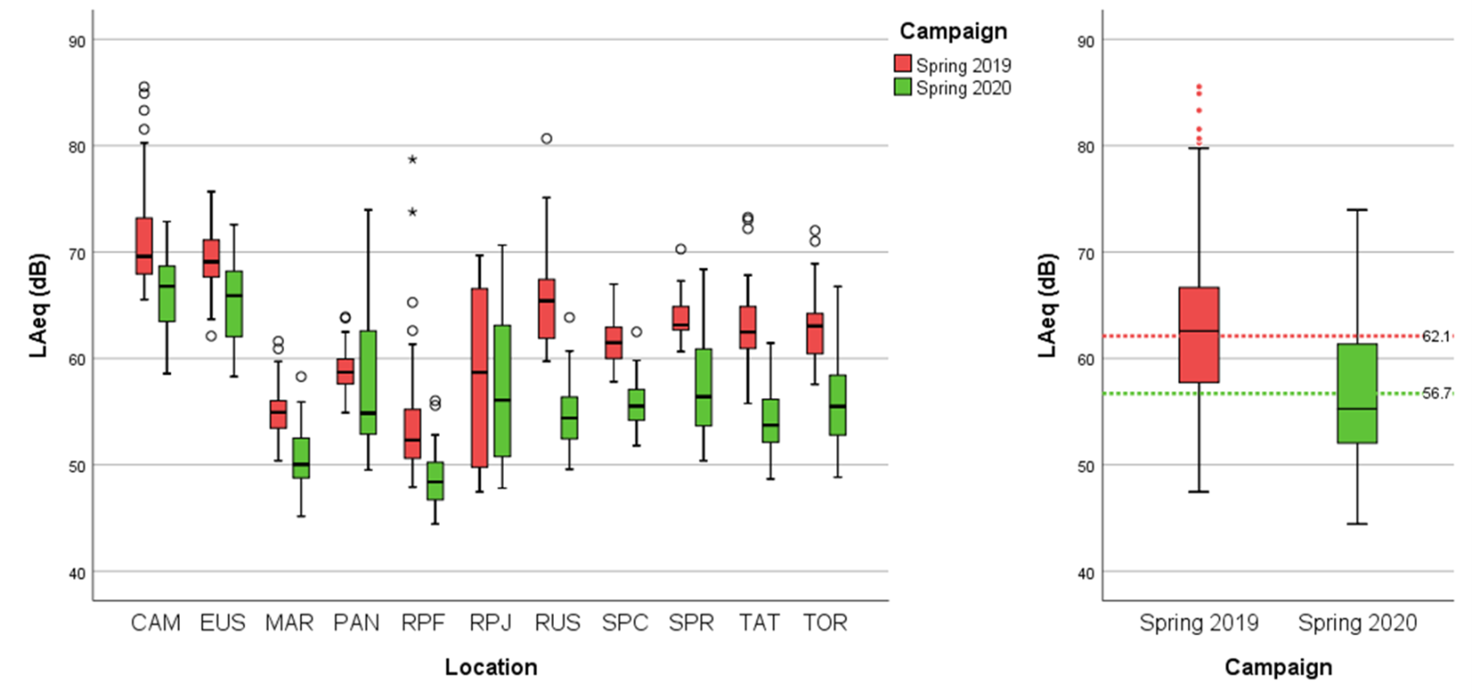
\includegraphics[width=\textwidth]{Figures/NoiseMappingLockdown Fig 1.png}   
   \caption{Reproduced with permission from \citet{Aletta2020Assessing}. On the left: Sound levels distributions at the 11 London locations before and during the lockdown measures implementation; on the right: Sound levels distributions (aggregated across locations) and corresponding mean values before and during the lockdown measures implementation. \label{fig:NsMapLockLAeq}}

   
  \end{figure}

%TODO: Discuss LAeq figure results in own wods

\begin{figure}[h]
  \centering
  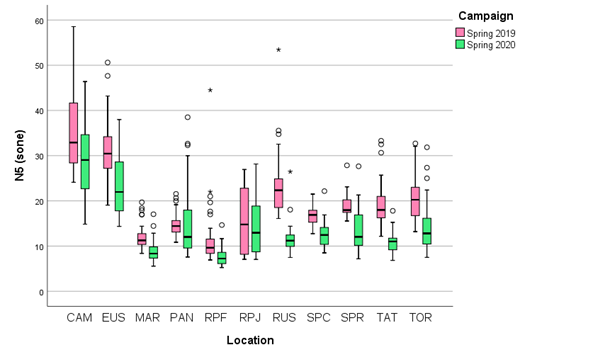
\includegraphics[width=.75\textwidth]{Figures/NoiseMappingLockdown Fig 4.png}
  \caption{Reproduced with permission from \citet{Aletta2020Assessing}. Loudness distributions at the 11 London locations before and during the lockdown measures implementation. \label{fig:NsMapLockN5}}

\end{figure}

%TODO: Discuss N5 figure in own words

\begin{figure}[h]
  \centering
  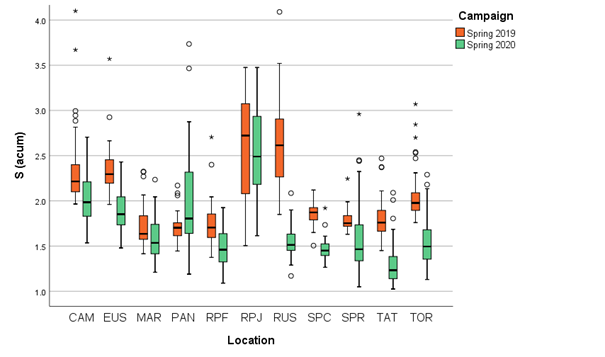
\includegraphics[width=.75\textwidth]{Figures/NoiseMappingLockdown Fig 5.png}
  \caption{Reproduced with permission from \citet{Aletta2020Assessing}. Sharpness distributions at the 11 London locations before and during the lockdown measures implementation. \label{fig:NsMapLockS}}

\end{figure}

%TODO: Discuss S figure in own words


\paragraph*{Effect of the urban setting on sound levels reduction}
In addition to strictly documenting the changes in the sound environment in London, the study also aimed to investigate whether the lockdown measures would result in different sound level reductions depending on the urban scenario (and its composition of sound sources). For this purpose, it was decided to define an "Area type" variable that would serve as a proxy for urban (acoustic) context: a \emph{k}-means cluster analysis was performed on the mean values of \gls{laeq}, \gls{la10}, \gls{la90}, \gls{n5}, and \gls{s} of the 2019 measurements campaign for the 11 locations, after those have been \emph{z}-score standardized to meet the algorithm criteria. The rationale was that clustering urban areas \emph{a priori} based on their "typical" acoustic climate (hence using only data from 2019) would allow us to see whether there was an association between area type and noise reduction. The algorithm was set to a three-cluster solution, based on visual inspection of the scree plot as reported in \cref{fig:NsMapLockScree} ("elbow method") \cit{33}. The analysis was conducted in R \cit{RStats} and figures were produced using the package factoextra \cit{factoextra}. 

\begin{figure}[h!]
  \centering
  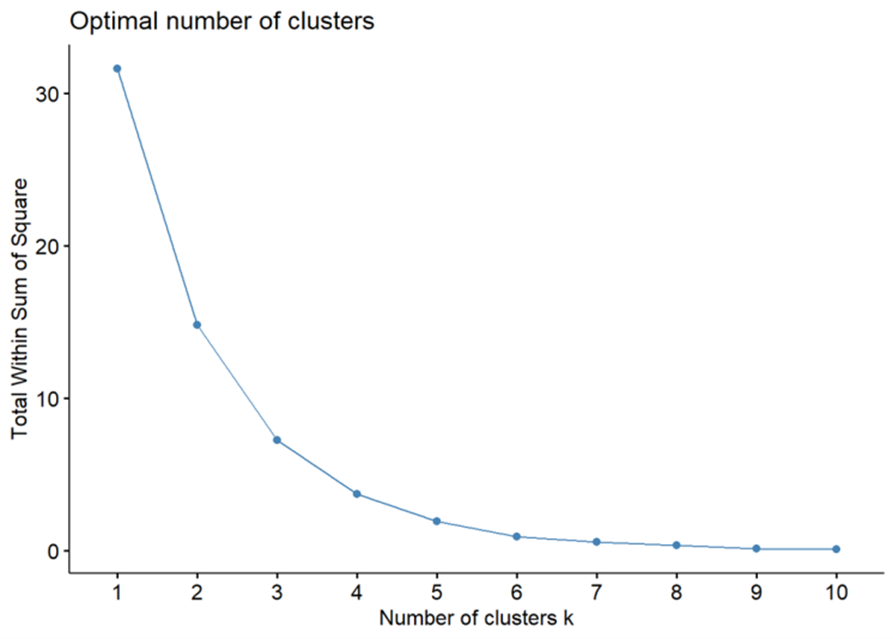
\includegraphics[width=.75\textwidth]{Figures/NoiseMappingLockdown Fig 6.png}  
  \caption{Reproduced with permission from \citet{Aletta2020Assessing}. "Scree" plot used to identify the optimal number of clusters to use in the \emph{k}-means clustering algorithm where an "elbow" can be identified for a three-cluster solution. \label{fig:NsMapLockScree}}
\end{figure}

\cref{fig:NsMapLockBiplot} shows a plot of clustered data based on the two most relevant underlying dimensions for the three-cluster solution. Dimension 1 seems to describe a pattern related to sound level and associated metrics, whilst Dimension 2 is related to Sharpness. This is consistent with previous findings in literature where it was observed that when it comes to categorization and classification of urban acoustic environments based on objective features, most solutions are reduced to intensity- and spectral-related parameters \cit{36, 37}. 

\begin{figure}[h!]
  \centering
  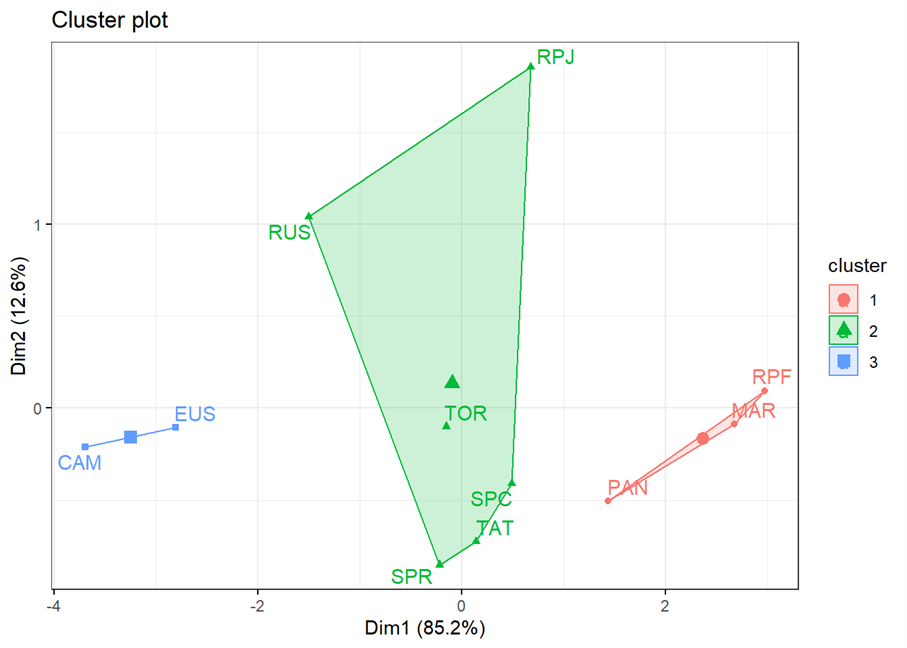
\includegraphics[width=\textwidth]{Figures/NoiseMappingLockdown Fig 7.png}  
  \caption{Reproduced with permission from \citet{Aletta2020Assessing}. Di-dimensional plot for the three-cluster solution. The clusters have been labelled as: Cluster 1 -- Quiet Areas; Cluster 2 -- Active Areas; Cluster 3 -- Traffic-dominated Areas. \label{fig:NsMapLockBiplot}}
\end{figure}

\cref{tab:NsMapLockClust} shows the basic descriptive statistics of the psychoacoustic features for the 11 locations according to cluster membership; when combining those patters with information about dominant sound sources as derived from data from \cit{26}, the three clusters could be labelled as: \emph{Traffic-dominated areas} (locations: Camden Town, Euston Tap), \emph{Active Areas} (locations: Regents Park Japan, Russell Square, St Pauls Cross, St Pauls Row, Tate Modern, Torrington Square) and \emph{Quiet Areas} (locations: Marchmont Garden, Pancras Lock, Regents Park Fields). Traffic-dominated areas are on major roads, where traffic noise is the dominant sound source. Active areas are locations where the human activity (also combined with traffic) is the main contributor to the acoustic environment. Quiet areas are generally parks or areas with greenery that tend to have a relatively low background noise (lack of traffic sources).

When considering the mean \gls{laeq} reductions between 2019 and 2020 as a function of Area type, it can be observed that they vary across the three clusters, as shown in Figure \cref{fig:NsMapLockRedux}. The biggest reductions are for Active areas (M = 6.6 dB; SD = 3.2 dB), followed by Traffic-dominated areas (M = 4.5 dB; SD = 0.8 dB), and Quiet areas (M = 3.6 dB; SD = 1.9 dB). A possible explanation for this is that road traffic at the selected locations in London is still sustained to some extent (e.g. circulation of public transport, key workers, etc.), while the most significant variation in Active areas is possibly due to the complete lack of (non-motorized) human activity on site. The locations in the cluster labelled as Quiet areas were already not particularly noisy even before the lockdown, thus the small changes observed are probably once again due to the absence of people.

%TODO: Reproduce the table from Aletta2020

\begin{table}[h]
\centering
\caption{Reproduced with permission from \citet{Aletta2020Assessing}. Sharpness distributions at the 11 London locations before and during the lockdown measures implementation.}
\label{fig:NsMapLockS}
\resizebox{\linewidth}{!}{%
\begin{tabular}{llrrrrr} 
\toprule
\textbf{Cluster} & \textbf{Parameter} & \multicolumn{5}{c}{\textbf{Mean values }} \\ 
\cline{3-7}
 &  & \multicolumn{1}{c}{$L_{Aeq}$} & \multicolumn{1}{c}{$L_{A10}$} & \multicolumn{1}{c}{$L_{A90}$} & \multicolumn{1}{c}{$S$} & \multicolumn{1}{c}{$N_5$} \\ 
\hline
1 -- (Quiet areas) & Mean & 55.9 & 58.1 & 52.4 & 1.7 & 12.9 \\
{[}N=3] & Std. deviation & 2.6 & 2.5 & 3.1 & 0.0 & 1.8 \\
 & Variance & 7.0 & 6.3 & 9.3 & 0.0 & 3.1 \\ 
\hline
2 -- (Active areas) & Mean & 62.5 & 64.3 & 59.6 & 2.1 & 18.9 \\
{[}N=6] & Std. deviation & 2.3 & 2.5 & 2.3 & 0.4 & 2.5 \\
 & Variance & 5.3 & 6.4 & 5.5 & 0.1 & 6.3 \\ 
\hline
3 -- (Traffic-dominated areas) & Mean & 70.4 & 72.9 & 66.1 & 2.4 & 34.1 \\
{[}N=2] & Std. deviation & 1.6 & 1.9 & 0.3 & 0.0 & 4.4 \\
 & Variance & 2.4 & 3.6 & 0.1 & 0.0 & 19.8 \\
\bottomrule
\end{tabular}
}
\end{table}

\begin{figure}[h]
  \centering
  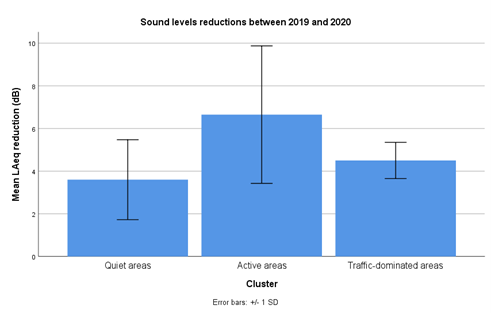
\includegraphics[width=\textwidth]{Figures/NoiseMappingLockdown Fig 8.png}
  \caption{Reproduced with permission from \citet{Aletta2020Assessing}. Mean A-weighted equivalent sound level reductions between the pre- and during-lockdown conditions as a function of cluster membership (i.e. Area type). \label{fig:NsMapLockRedux}}
\end{figure}


 This study revealed that average reductions in the various locations considered ranged from 10.7 dB (\gls{laeq}) to 1.2 dB, with an overall average reduction of 5.4 dB. This metric-reporting focussed approach left the following research questions unanswered:
 \begin{enumerate}
   \item How would people have perceived these spaces as a result of this change in acoustic environment? (RQ1)
   \item Would these sound level reductions result in improvements to the soundscape of the spaces? (RQ2)
 \end{enumerate}

 The \nth{1} research question (RQ1), addressing the perceptual effect of the change in urban soundscape induced by the lockdowns, can be further broken down into the following questions:

 \begin{itemize}
   \item How was the sound source composition influenced by the change?
   \item How would the affective response to the acoustic environment in lockdowns change?
   \item Could this demonstrate the effect of human activities on the perception of an acoustic environment in general?
 \end{itemize}


 \subsection{Review of predictive modelling}
 These questions arise out of the soundscape approach, which is characterised by prioritising the perceptual effect of an acoustic environment by taking into account the interaction of sound sources, context, and the person perceiving it \citep{ISO12913Part1,Truax1999Handbook}, bringing together objective and subjective factors. The soundscape approach to noise mitigation and management is being recognised as a response to arising environmental requirements on noise pollution and sustainability, such as the regulation of quiet areas in Europe \citep{EEA2020Environmental, Aletta2018Towards,Radicchi2021Sound}. This has been further formalised in \citet{ISO12913Part2} via the adoption of the circumplex model of soundscape \citep{Axelsson2010principal}, in which the perception of a soundscape can be described in terms of its pleasantness and eventfulness, as one of the standard methods of soundscape assessment.

 Soundscape research is therefore traditionally rooted in environmental acoustics and environmental psychology, typically dealing with outdoor spaces \citep{Torresin2020Indoor} and urban open spaces, where parks and squares are often used as case study sites \citep{Kang2007Urban}. A soundscape assessment typically requires people to be surveyed but the presence of people at a location influences assessment \citep{Aletta2018Towards} and 'quiet places' usually require low numbers of users to remain quiet, which limits the possibility of an assessment. Even in a crowded public space, soundscape surveys are demanding as they require significant resources to carry out at scale, limiting their widespread application \citep{Mitchell2020Soundscape}. Therefore, a need for a predictive model arises to overcome this limitation and improve the implementation of the soundscape approach into everyday planning and management practices.

 According to a recent review of predictive soundscape models from \citet{Lionello2020systematic}, the degree of employing auditory and non-auditory factors in soundscape prediction varies with some studies relying on contextual \citep{Kajihara2017Imaginary}, personal/demographic \citep{Erfanian2021Psychological,Tarlao2020Investigating} or social media \citep{Aiello2016Chatty} data entirely to predict and generate soundscape features. Some methods also incorporate perceptually-derived features, such as subjective sound level and visual pleasantness as predictors \citep{Lionello2020systematic}. In general, these methods which incorporate perceptually-derived inputs achieve better accuracy rates than those which don't, however this information must also be obtained from people via a survey and therefore are unsuitable for predictive modelling where surveys are not possible. For example, \citet{Ricciardi2015Sound} proposed two models based on data collected from a smartphone application to predict urban sound quality indicators based on linear regressions. The first model which incorporated perceptually-derived input features (visual quality and familiarity) achieved an $R^2$ of 0.72, while a second model without these features achieved an $R^2$ of 0.58. This indicates the necessity for considering and accounting for the influence which contextual factors in a space have on the relationship between the sound environment itself and the listener's perception of it (i.e. the soundscape) while also highlighting the challenges associated with a predictive model which depends only on measurable features.

 Therefore, a third research question arises: what are the key features needed for a soundscape prediction model based on comprehensive acoustic on site measurements to be used for assessing locations with low social presence or in situations where conducting surveys is impractical (RQ3)?

\section{Materials and Methods}

 This study was conducted via initial onsite data collection campaigns in Central London and Venice in 2019 before the outbreak of \gls{covid19} as part of the \gls{ssid} project \citep{Mitchell2020Soundscape} and in 2020 during the strictest part of the lockdowns \citep{Aletta2020Assessing}, including objective acoustic data (2019 and 2020) and subjective responses (2019 only). The full in situ dataset, as described in this section, has been made publicly available as "The International Soundscape Database (V0.2.1)" on Zenodo (\url{https://zenodo.org/record/5654747}) \citep{Mitchell2021International}.
 
 Using both 2019 and 2020 binaural recordings, an online listening experiment was conducted to provide an understanding about the change in sound source composition. The 2019 onsite questionnaire data were used to define the dominant sound source at each location as a starting point for interpreting the soundscape change. A predictive model was developed to reveal the change in the perceived pleasantness and eventfulness using objective acoustic data and location to predict subjective responses. Although the initial (2019) dataset contains additional locations (specifically, in Spain, the Netherlands, and China), due to the nature of this study as a reaction to the strict movement and activity restrictions, the sites which could be included in the lockdown (2020) measurement campaigns were limited to locations where staff and equipment had access and where recordings could be undertaken during the spring of 2020.

 The sites were selected to provide a mixture of sizes and uses, varying in typology ranging from paved squares to small and large parks to waterside spaces across both cities. Throughout the text they are indexed via a LocationID based on the location's name (e.g. CamdenTown, SanMarco), while a more in-depth overview of each is given in supplementary files. %NOTE: Will need to adjust this within thesis.
 London is taken as an example of a large, typically noisy city while the Venice sample provides a unique look at spaces with typically very high human activity levels and no road traffic activity. In particular, the 2019 Venice surveys were taken to coincide with the yearly Carnevale festival in order to capture its distinct soundscape.

\citet{ISO12913Part2} was consulted for reporting on soundscape data. A detailed description of the 2019 survey campaigns in featured through the paper and in the public database. This study was approved by departmental UCL IEDE Ethics Committee on \nth{17} July 2018 for onsite data collection and on the \nth{2} of June 2020 for the online listening experiment and is conducted in adherence to the ethical requirements of the Declaration of Helsinki \citep{WMA2013World}.

 \subsection{Onsite data: Questionnaires, binaural measurements, and recordings}
   %FIXME: Likely will not need this within thesis.
   The initial onsite data collection featured both questionnaire data collected from the general public and acoustic measurements, conducted across thirteen urban locations (in London $N=11$, in Venice $N=2$) between the \nth{28} of February and the \nth{21} of June 2019, with additional sessions in July and October 2019. Although the total survey period in 2019 extended over several seasons, the surveys at any individual location did not extend over seasons with different occupancy patterns. A total of 1,318 questionnaire responses were collected from the general population across the measurement points during 1 -- 3 hour-long campaigns in both cities in 2019, accompanied by 693 approximately 30-second long 24-bit 44.1 kHz binaural recordings. After data cleaning, each of the 13 locations was characterised by between 14 to 80 recordings and between 24 to 147 questionnaire responses. Mean age of the participants was 33.9, with a standard deviation of 14.57 (45\% male, 53.8\% female, 0.4\% non-conforming, 0.9\% prefer-not-to-say).

   Although recent results from both \citet{Tarlao2020Investigating} and \citet{Erfanian2021Psychological} indicate the important influence of personal and demographic factors -- in particular age and gender -- on soundscape perception, these factors were not included as potential features in the modelling process. Given the nature of this study as addressing a scenario when people could not be surveyed, no additional demographic information is available in the lockdown case to be fed into the model and is therefore not useful to include for the development and application of this specific predictive model. This information is reported throughout the study simply to provide further context to the data collection.

   The subsequent measurement campaign in 2020 mimicked the binaural recording strategy applied in the initial campaign and was performed between the \nth{6} and the \nth{25} of April 2020 in both cities, this time excluding the questionnaire. An additional 571 binaural recordings were collected on site in 2020.

   \subsubsection{Data collection}
   %FIXME: Probably don't need this section in thesis either.
   The 2019 data collection was performed across all the locations using the protocol based on the Method A of the ISO/TS 12913-2:2018 \citep{ISO12913Part2}, as described in \citep{Aletta2020Assessing,Mitchell2020Soundscape}, collected either via handheld tablets or paper copies of the questionnaire. The full questionnaire and data collection procedure are given in \citet{Mitchell2020Soundscape}, however the key parts used for this study are those addressing sound source dominance and \gls{paq}.
   %NOTE: Skipping next section since it's detailed earlier in thesis.

   %NOTE: add a section to the methods about the projection. Heavy reference to / pulling from Lionello 2020 and JASA-EL paper.
   In order to simplify the results and allow for modelling the responses as continuous values, the 8 \glspl{paq} undergo a trigonometric projection to reduce them onto the two primary dimensions of pleasant and eventful, according to the procedure outlined in Part 3 of the ISO 12913 series \citep{ISO12913Part3}. In order to distinguish the projected values from the Likert-scale \gls{paq} responses, the projected values will be referred to as \gls{isopl} and \gls{isoev} and can be considered to form an x-y coordinate point (x = \gls{isopl}, y = \gls{isoev}) as explained in detail in \citet{Lionello2021Introducing}.

   %NOTE: Skipping paragraph on binaural recording info

   \subsubsection{Data cleaning}
   %TODO: Move and expand this data cleaning section to the methods section
   The cleaning of the samples was conducted using the ArtemiS SUITE 11. The researcher discarded or cropped whole recordings, or its parts affected by wind gusts or containing noises and speech generated by the recording operator by accident or for the purpose of explaining the questionnaire to a participant. This resulted in 1,291 binaural recordings which were then processed further, as described in \cref{sec:analyses}. Psychoacoustic analyses are shown in the publicly available database.

   In order to maintain data quality and exclude cases where respondents either clearly did not understand the \gls{paq} adjectives or intentionally misrepresented their answers, surveys for which the same response was given for every \gls{paq} (e.g. 'Strongly agree' to all 8 attributes) were excluded prior to calculating the ISO projected values. This is justified as no reasonable respondent who understood the questions would answer that they 'strongly agree' that a soundscape is pleasant and annoying, calm and chaotic, etc. Cases where respondents answered 'Neutral' to all \glspl{paq} are not excluded in this way, as a neutral response to all attributes is not necessarily contradictory. In addition, surveys were discarded as incomplete if more than 50\% of the \gls{paq} and sound source questions were not completed. The site characterisation per \citet{ISO12913Part2} is available in the supplementary files, featuring the address, overall psychoacoustic characteristics of the location, typical use of each location, and pictures taken during the survey sessions.

   \subsubsection{Psychoacoustic analyses}
   \label{sec:analyses}
   %NOTE: May want to move this to methods as well.
   The binaural recordings were analysed in ArtemiS SUITE 11 to calculate the suite of 11 acoustic and psychoacoustic features given in \cref{tab:psychoacoustics} to be used as initial predictors.

\begin{table}[h!]
  \centering
  \caption{Psychoacoustic features considered for inclusion in the predictive models. All metrics are calculated for the full length of the recording (30s). As recommended by \citet{ISO532Part1} and \citet{ISO12913Part2}, the \nth{5} percentile of Loudness is used rather than the average. \label{tab:psychoacoustics}}
  % \resizebox{\linewidth}{!}{%
    \begin{tabular}{lccl}
      \toprule
      \textbf{Feature}                                                      & \textbf{Symbol} & \textbf{Unit} & \textbf{Calculation Method}       \\
      \midrule
      \begin{tabular}[c]{@{}l@{}}Loudness \\(fifth percentile)\end{tabular} & $N_5$           & sones         & \citet{ISO532Part1}               \\
      Sharpness                                                             & $S$             & acum          & \citet{ISO532Part1}               \\
      Roughness                                                             & $R$             & asper         & \citet{ECMA418Part2}              \\
      Impulsiveness                                                         & $I$             & iu            & \citet{ECMA418Part2}              \\
      Fluctuation Strength                                                  & $FS$            & vacil         & \citet{ECMA418Part2}              \\
      Tonality                                                              & $T$             & tuHMS         & \citet{Sottek2016Hearing}        \\
      \begin{tabular}[c]{@{}l@{}}Psychoacoustic \\Annoyance\end{tabular}    & $PA$            & –             & \citet{PsychoacousticsfactsmodelsZwicker} \\
      $L_{Aeq}$                                                               & $L_{Aeq}$         & dB            & \citet{IEC61672Part1}      \\
      $L_{A10}-L_{A90}$                                                         & $L_{A10}-L_{A90}$   & dB            & \citet{ISO1996Part1}             \\
      $L_{Ceq}-L_{Aeq}$                                                         & $L_{Ceq}-L_{Aeq}$   & dB            & \citet{ISO1996Part1}             \\
      Relative Approach                                                     & $RA$            & cPA           & \citet{Sottek2005Models}          \\
      \bottomrule
    \end{tabular}
  % }
\end{table}

   The (psycho)acoustic predictors investigated were selected in order to describe many aspects of the recorded sound -- in particular, the goal was to move beyond a focus on sound level, which currently dominates the existing literature on the acoustic effects of lockdowns noted in \ref{sec:intro}. In all, they are expected to reflect the sound level (\gls{laeq}), perceived sound level (gls{n5}), spectral content (\gls{s}, \gls{lcla}, \gls{tu}), temporal character or predictability (\gls{iu}, \gls{fs}, \gls{ra}), and overall annoyance (\gls{pa}). These metrics have been proposed as indicators to predict perceptual constructs of the soundscape \citep{Aletta2017Dimensions, Aletta2016Soundscape} and have shown promise when combined together to form amore comprehensive model applied to real-world sounds \citep{Orga2021Multilevel}. The maximum value from the left and right channels of the binaural recording are used, as suggest in ISO/TS 12913-3:2019 \citep{ISO12913Part3}.

   %FIXME: Fix layout of correlation table
% \usepackage{booktabs}
% \usepackage{rotating}


\begin{sidewaystable}[hp]
\centering
\caption{Pearson correlation coefficients between candidate acoustic features and ISOPleasant and ISOEventful across all 13 locations. Only statistically significant ($p < 0.01$) coefficients are shown. \label{tab:corr}}
\begin{tabular}{r|cccccccccccc} 
\toprule
\textbf{Parameter} & ISOPl & ISOEv & $PA$ & $N_5$ & $S$ & $R$ & $I$ & $FS$ & $T$ & $L_{Aeq}$ & $L_{A10}-L_{A90}$ & $L_{Ceq}-L_{Aeq}$ \\ 
\midrule
ISOPleasant &  &  &  &  &  &  &  &  &  &  &  &  \\
ISOEventful & -0.24 &  &  &  &  &  &  &  &  &  &  &  \\
$PA$ & -0.28 & 0.24 &  &  &  &  &  &  &  &  &  &  \\
$N_5$ & -0.37 & 0.33 & 0.94 &  &  &  &  &  &  &  &  &  \\
$S$ &  &  & 0.71 & 0.56 &  &  &  &  &  &  &  &  \\
$R$ & -0.36 & 0.32 & 0.63 & 0.74 & 0.11 &  &  &  &  &  &  &  \\
$I$ &  &  & -0.10 &  & -0.37 & 0.24 &  &  &  &  &  &  \\
$FS$ & -0.11 & 0.14 & 0.37 & 0.43 &  & 0.46 & 0.55 &  &  &  &  &  \\
$T$ & -0.21 & 0.30 & 0.58 & 0.63 & 0.12 & 0.54 & 0.16 & 0.52 &  &  &  &  \\
$L_{Aeq}$ & -0.34 & 0.37 & 0.84 & 0.93 & 0.56 & 0.72 & -0.09 & 0.37 & 0.57 &  &  &  \\
$L_{A10}-L_{A90}$ & -0.18 & 0.15 & 0.21 & 0.33 & -0.20 & 0.31 & 0.36 & 0.44 & 0.40 & 0.23 &  &  \\
$L_{Ceq}-L_{Aeq}$ &  & -0.20 & -0.49 & -0.49 & -0.54 & -0.31 &  & -0.27 & -0.28 & -0.61 & -0.22 &  \\
$RA$ & -0.34 & 0.31 & 0.60 & 0.74 & 0.18 & 0.71 & 0.31 & 0.63 & 0.58 & 0.73 & 0.23 & -0.14 \\
\bottomrule
\end{tabular}
\end{sidewaystable}


   \cref{tab:corr} shows the Pearson correlation coefficient between each of the candidate acoustic features and the outcome pleasantness and eventfulness. For \gls{isopl} ($ISOPl$), we can perhaps see three tiers of correlations:

   \begin{enumerate}
     \item The more highly correlated tier ($|r| > 0.28$) consists of \gls{ra}, \gls{laeq}, \gls{r}, \gls{n5}, and \gls{pa}
     \item The low correlation tier consists of \gls{la10la90}, \gls{tu}, and \gls{iu}
     \item \gls{lcla}, \gls{iu}, and \gls{s} show no correlation
   \end{enumerate}

   For \gls{isoev} ($ISOEv$), these tiers are:
   \begin{enumerate}
     \item The more highly correlated tier ($|r| > 0.30$) consists of \gls{ra}, \gls{laeq}, \gls{tu}, \gls{r}, and \gls{n5}
     \item The low correlation tier consists of \gls{lcla}, \gls{la10la90}, \gls{fs}, and \gls{pa}
     \item \gls{iu} and \gls{s} show no correlation
   \end{enumerate}

   Among the correlations for the psychoacoustic metrics considered for inclusion as input features, we can see several highly inter-correlated features. As expected, \gls{pa}, \gls{laeq}, and \gls{n5} are highly correlated, meaning that careful consideration is paid to these features to ensure they do not contribute to multicollinearity in the final model.

 \subsection{Modelling}

   Two linear multi-level models (MLM) were computed to predict: 1) \gls{isopl}, and 2) \gls{isoev}. The inherent grouped structure of the \gls{ssid} database necessitates a modelling and analysis approach which considers the differing relationships between the objective acoustic features and the soundscape's perceived affective quality ratings across the various locations and contexts. The individual-level of the models is made up of the acoustic features calculated from the binaural recordings made during each respondent's survey period, while the group-level includes the categorical 'LocationID' variable indicating the location in which the survey was taken, acting as a non-auditory contextual factor.

   A separate backwards-step feature selection was performed for each of the outcome models in order to identify the minimal feature set to be used for predicting each outcome. In this feature selection process, an initial model containing all of the candidate features was fit. Each feature was then removed from the model one at a time, then the best-performing model is selected and the procedure continues step-wise until no improvement is seen by removing more features. This process is carried out first on the location-level features (including the potential to remove all features including LocationID, resulting in a 'flat' or standard multivariate linear regression model), then on the individual-level features. The performance criterion used for this process was the \gls{aic} \citep{Akaike1974New}. To check for multicollinearity among the selected features, the \gls{vif} was calculated and a threshold of $\gls{vif} < 5$ was set. Any features which remained after the backwards step-wise selection and which exceeded this threshold were investigated and removed if they were highly collinear with the other features.

   All of the input features are numeric values, in the units described above. Before conducting feature selection, the input features are z-scaled to enable proper comparison of their effect sizes. After the feature selection, the scaled coefficients are used in the text when reporting the final fitted models to facilitate discussion and comparison between the features. The unscaled model coefficients are reporting in \draft{Appendix B} to enable the models to be applied to new data. In order to properly assess the predictive performance of the model, an 80/20 train-test split with a balanced shuffle across LocationIDs was used. The z-scaling and feature selection were performed on the training set only, in order to prevent data leakage. To score the performance of the model on the training and testing sets, we use the \gls{mae}, which is in the scale of the response feature -- for \gls{isopl} and \gls{isoev} this means our response can range from $-1$ to $+1$. However, since the end-goal of the model is to predict the soundscape assessment of the location as a whole, rather than the individual responses, we also assess the performance of the model in predicting the average response in each location. To do this, the mean response value for each location is calculated, and the $R^2$ accuracy across LocationIDs is reported for both the training and testing sets.

   The model fitting and feature selection was performed using the `step` function from `lmerTest` (v3.1.3) \citep{Kuznetsova2017lmerTest} in R statistical software (v.4.0.3) \citep{RCT2021R}. The summaries and plots were created using the `sjPlot` package (v.2.8.6) \citep{Luedecke2021sjPlot} and `seaborn` (v.0.11.1) \citep{Waskom2021seaborn}.

 \subsection{Online Survey}

   A online listening test was conducted using the Gorilla Experiment Builder \href{www.275gorilla.sc}{} \citep{AnwylIrvine2020Gorilla}. The participants were exposed to a random selection of 78 binaural recordings (39 from 2019 and 39 from 2020, 6 recordings per location). Each participant had the option to evaluate either 1 or 2 sets of 6 recordings randomly assigned between 13 stimuli sets. Mp3 files, converted at 256 kBps were used due to the requirements of the Gorilla platform.

   No visual stimuli were used in the experiment. The experiment consisted of:

   \begin{enumerate}
     \item an initial exercise to enhance the chances of participants complying with the instructions and wearing headphones
     \item a training set using two randomly chosen binaural recordings (then not used in the main task) from the dataset
     \item a soundscape characterisation questionnaire starting with an open-ended question about perceived sound sources and featuring the same questions as the one used in-situ, looking into the perceived sound source dominance of the following four types: traffic noise, other noise, human sounds, and natural sounds
     \item a questionnaire on the basic demographic factors.
   \end{enumerate}

   The questionnaire used in Part 3 of the online experiment is report in \draft{Appendix A}.

   Having in mind the remote nature of the study and to ensure a minimum level of robustness for reliable sound source recognition, an initial exercise was performed consisting of a headphone screening test \citep{Woods2017Headphone} and a headphone reproduction level adjustment test \citep{Gontier2019Estimation}. The level adjustment was performed using an 11-second-long pink noise sample matched to the lowest and the highest \gls{la90} values from the experimental set. Participants were asked to adjust their listening level to clearly hear the quieter sample while keeping the level low enough, so they don't find the louder sample disturbing. The headphone screening test followed, featuring a stereo signal of 1-second-long 100 Hz sin tone, generated with Izotope RX6 application, played at a 3 dB difference where one of the equally loud pairs had its phase inverted. A 100 Hz sin was used because the pilot tests revealed that the 200 Hz sin tone proposed by \citet{Woods2017Headphone} created a higher uncertainty varying across different laptop models and would likely contribute to the chances of a participant fooling the test. It was expected that participants using speakers would not be able to either hear the sin wave or would be fooled by the inverted phase effect and therefore not able to pass the trials, unless they were indeed using headphones. The participant needed to recognise the quietest of the 3 samples in a trial of 6 attempts. Only participants correctly answering 5 or more out of 6 trials were allowed to proceed with the experiment. Participants were asked not to change their audio output settings during the rest of the experiment. This was introduced to ensure that a participant is using a headphone playback system which allows a listener to clearly recognise a 3 dB difference at 100 Hz as a proxy for sufficient audio quality playback.

   Online questionnaire data was collected between the \nth{9} of June and the \nth{9} of August 2020. Within the Gorilla Experiment Builder, a total of 250 attempts to complete the experiment were recorded, where 165 participants were excluded either on the basis of not passing the headphone screening ($N=79$) or for not completing the experiment, usually before engaging into the screening ($N=83$). Out of a total of 88 participants who completed the test, 2 participants were excluded as outliers as they provided uniform answers across all the questions and commented on not being able to properly hear the stimuli, despite their successful completion of the training tests. The participants of the online experiment were of mean age 32.42, 45.1\% male, 54.9\% female.

   \cref{fig:lockdown-study-framework} illustrates and summarises the framework and sections described above.

   \begin{figure}[h]
     \centering
     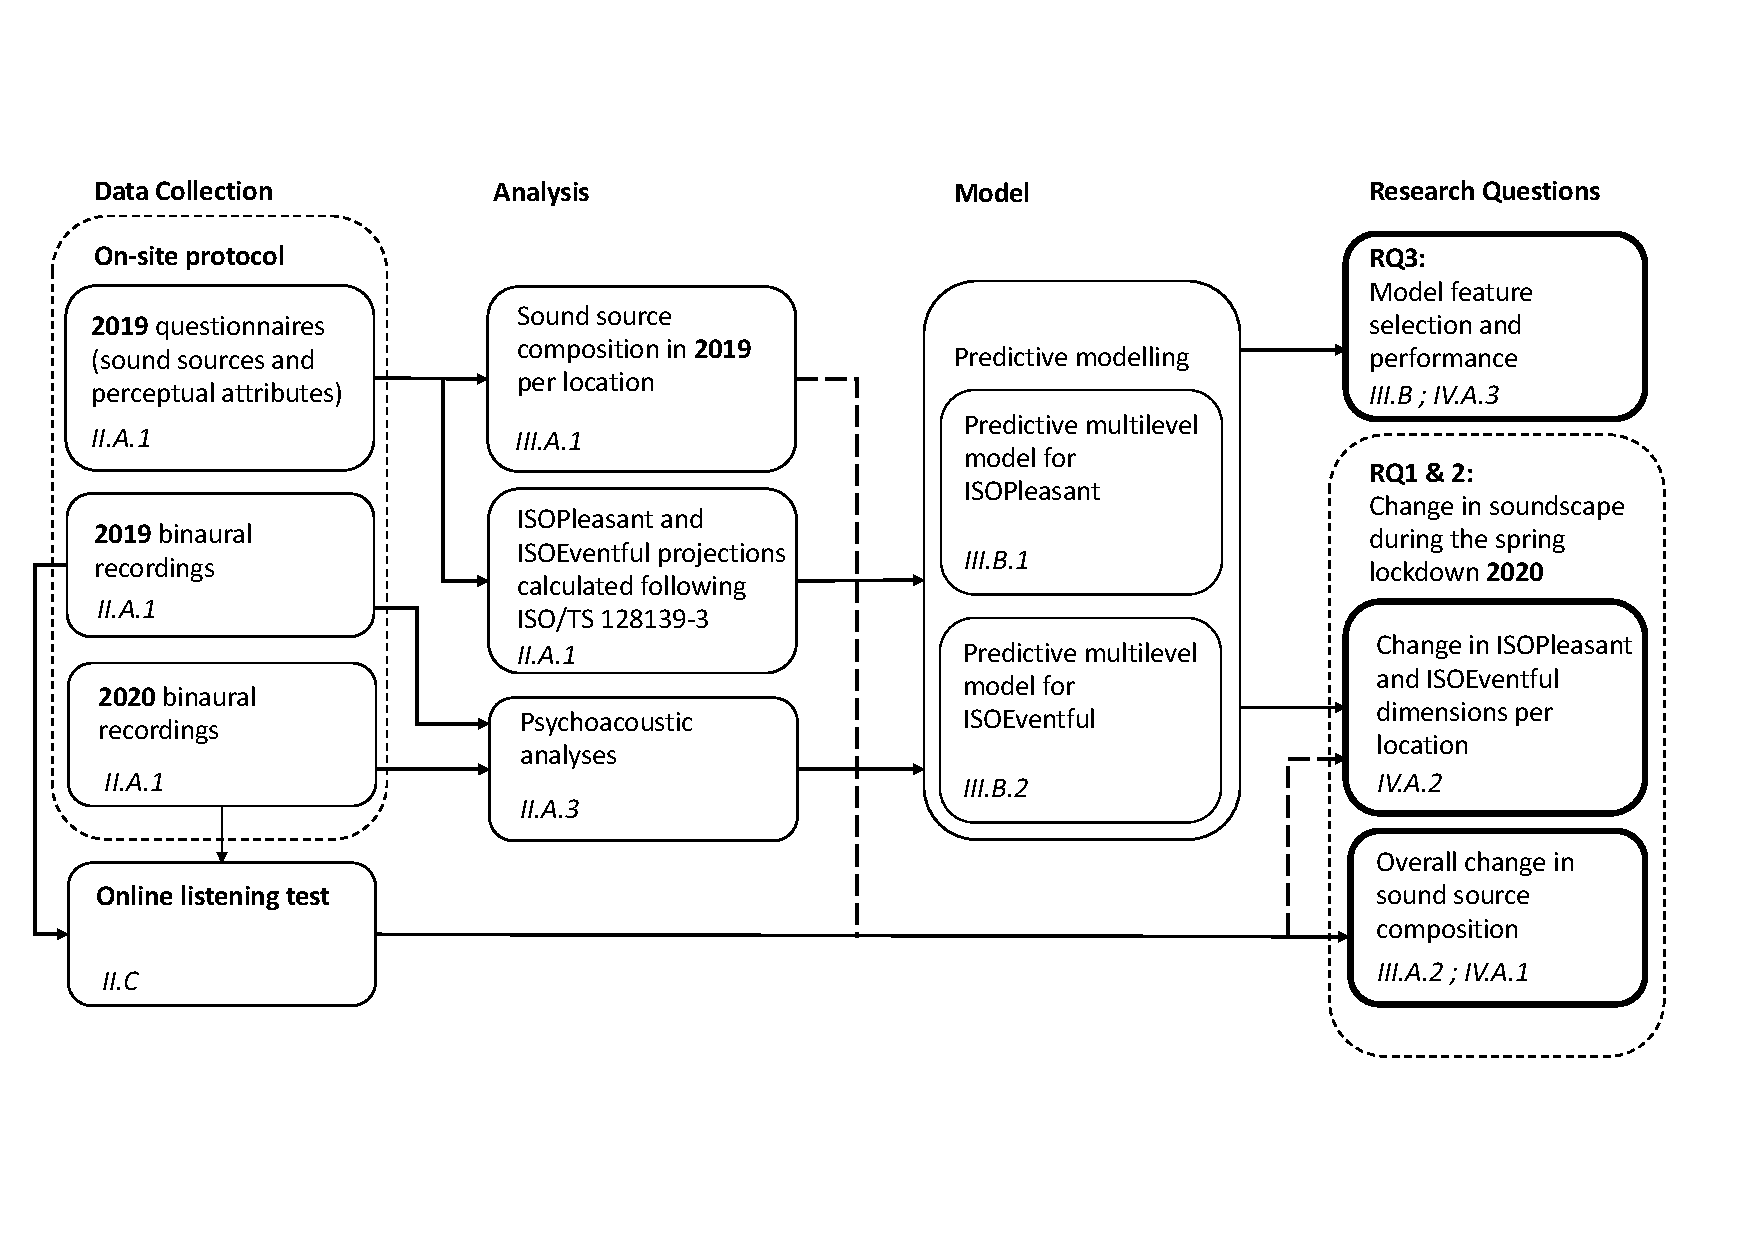
\includegraphics[width=\textwidth]{Figures/Lockdown-Fig1.pdf}
     \caption{The study flowchart indicating the data collection, analysis, modelling, and discussion throughout the study. The subsections in the text to which each box refers are indicated in italics. \label{fig:lockdown-study-framework}}
     %FIXME: Change the section references to match.
   \end{figure}

\section{Results}

 The results of the onsite surveys, online experiment, and the model development are reported here. They are reported following the structure of the ISO/TS 12913 series, revealing the perceived sound source dominance, key perceptual attributes (\gls{isopl} and \gls{isoev}) and the lockdown-related changes.

 \subsection{Perceived sound source dominance}

   \subsubsection{2019 sound source composition per location}

   Questionnaire data was collected English, Italian, and Spanish in both cities. The respective questionnaires can be found in the supplementary files and \citet{Mitchell2020Soundscape}. Data presented here was aggregated per LocationID.

   According to the highest scored mean value of the dominant sound source type, as shown in \cref{fig:sound-source-dom}, the locations can be grouped into: natural sounds dominated (RegentsParkJapan, RegentsParkFields, RussellSq), human sounds dominated (SanMarco, TateModern, StPaulsRow, StPaulsCross, MonumentoGaribaldi), noise (traffic and other noise) sounds dominated (CamdenTown, EustonTap, TorringtonSq, PancrasLock).

   \begin{figure}[h]
     \centering
     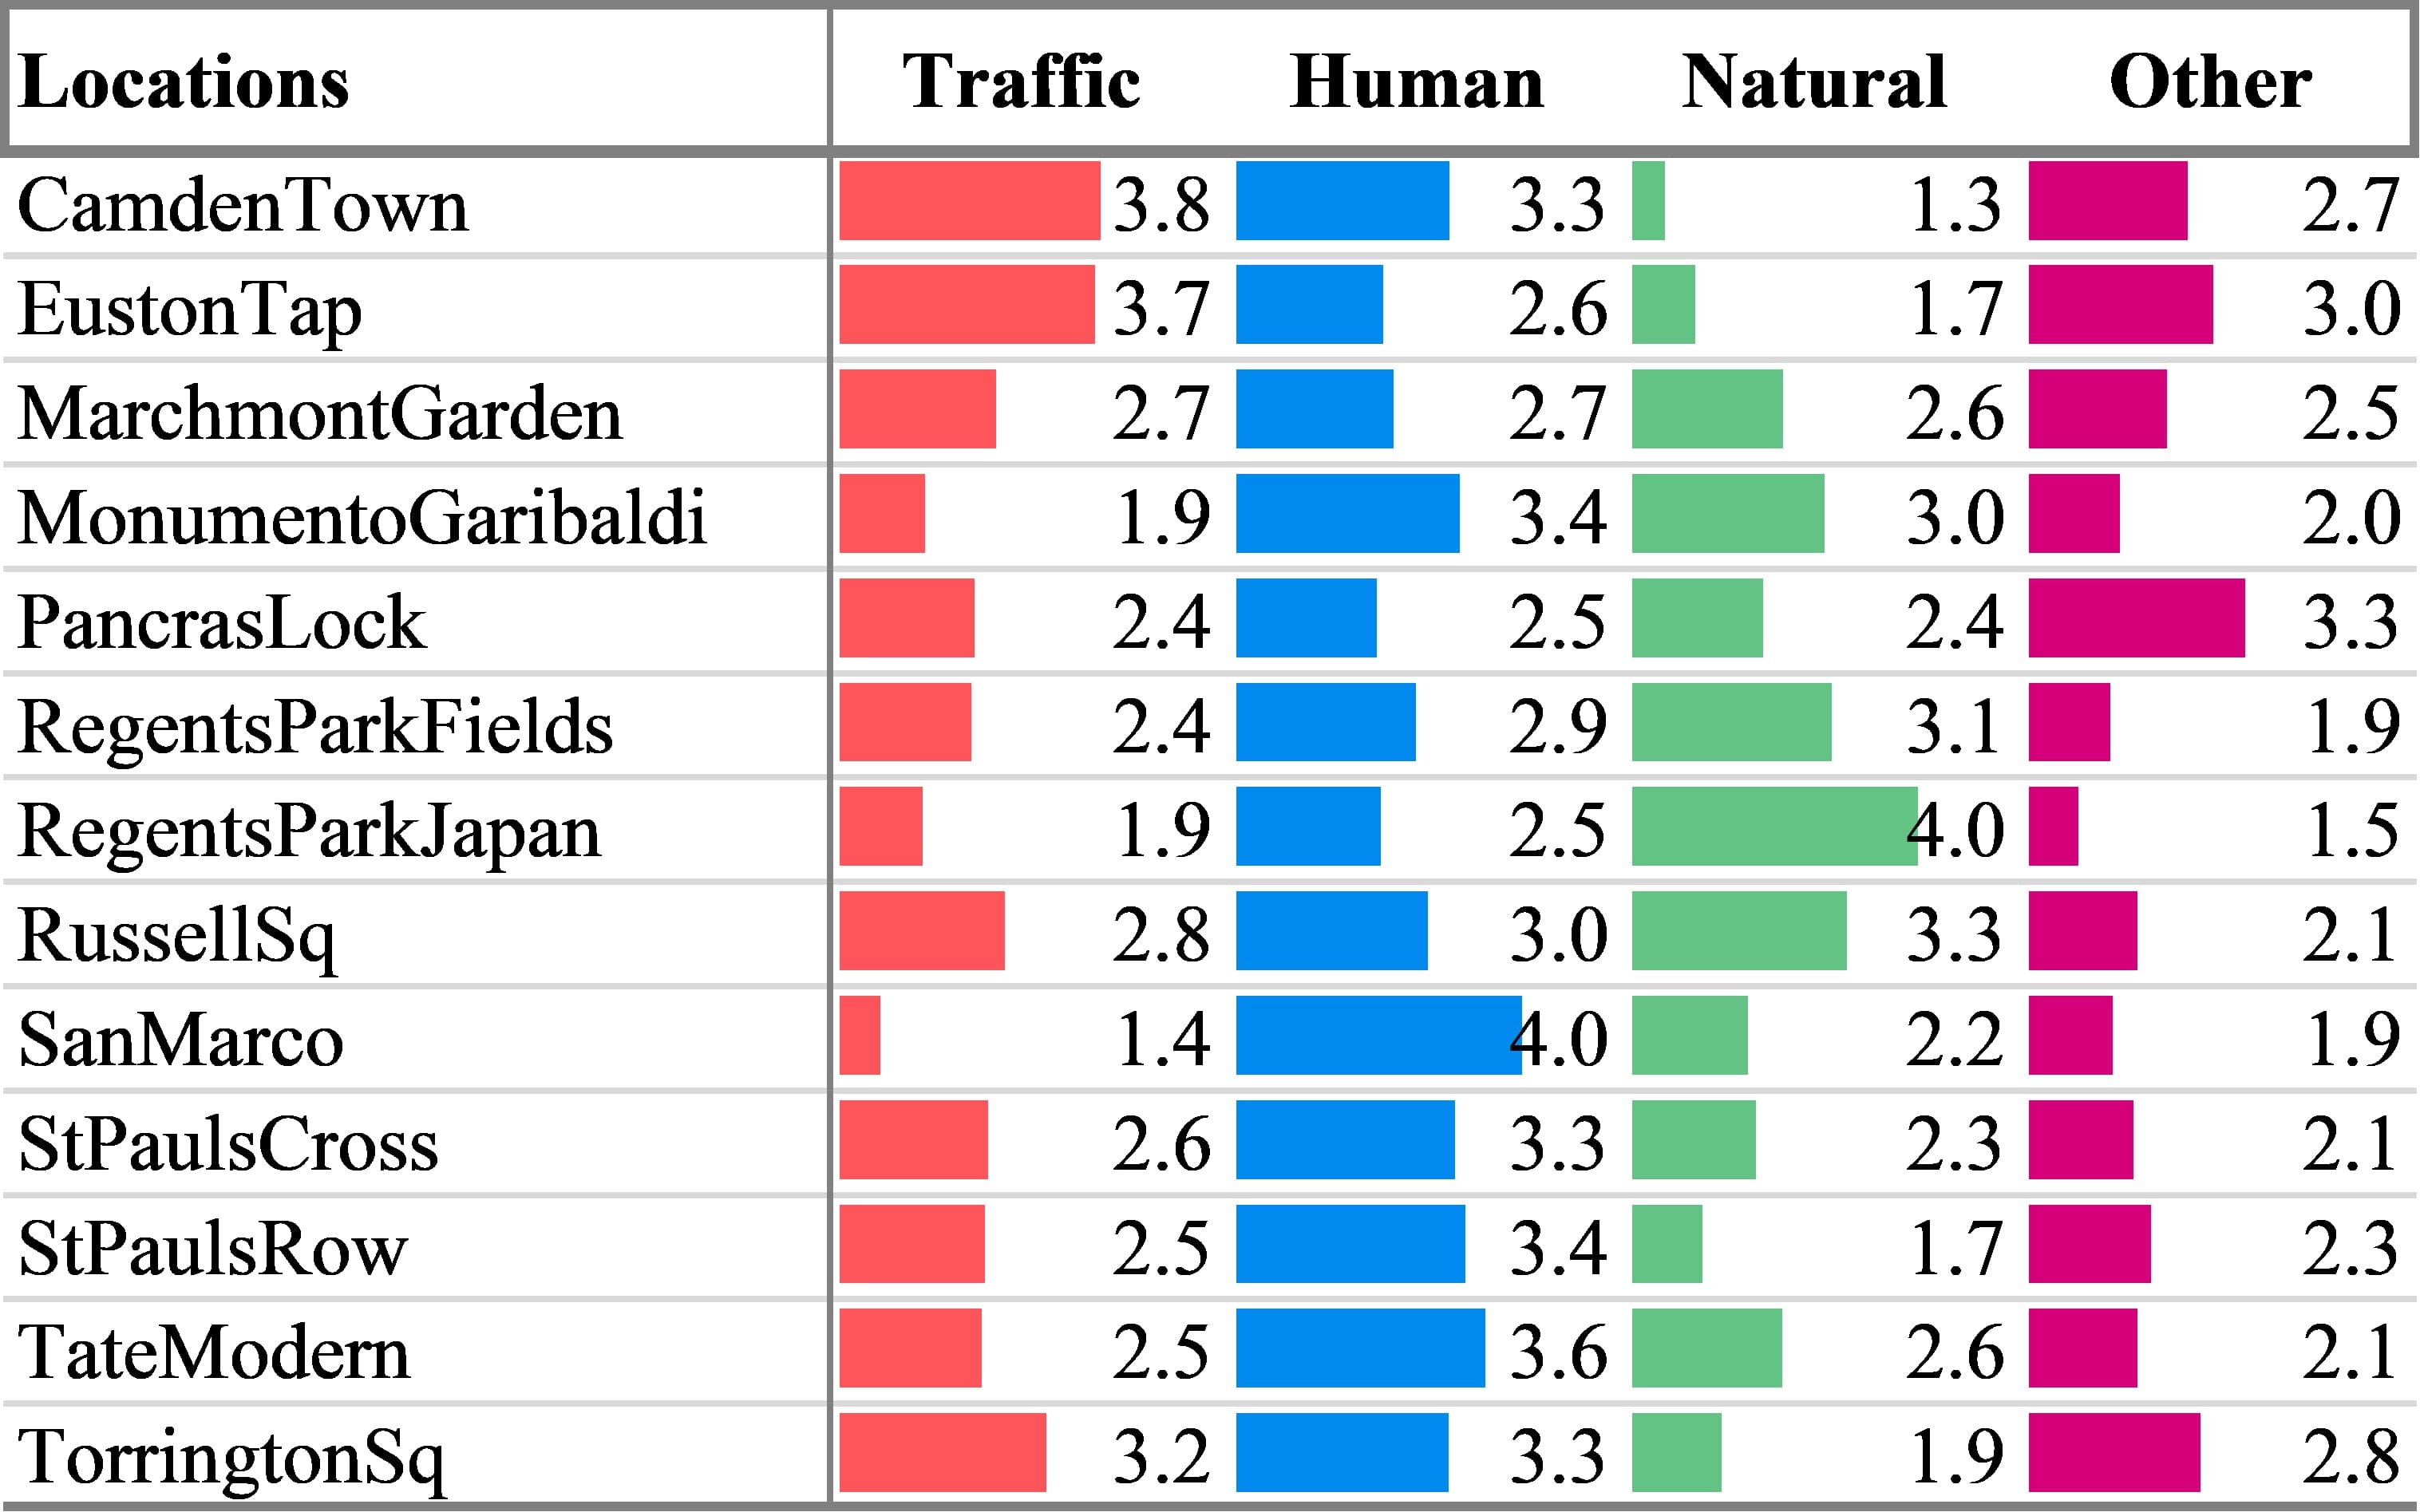
\includegraphics[width=.8\textwidth]{Figures/Lockdown-Fig2.jpg}
     \caption{Mean values per LocationID for the perceived dominance of the sound source types, for the 2019 on-site campaign. \label{fig:sound-source-dom}}
   \end{figure}

   \subsubsection{Overall change in the perceived sound source dominance during lockdown}

   1,803 words describing the sound sources present in the 2019 recordings and 1,395 words related to the 2020 recordings were input by participants in response to the open-ended question Q1 \draft{(see Appendix A)}. The frequency of occurrence, generated using the Word-Clouds web app, is shown in Figure \cref{fig:wordclouds}, for the 2019 and the 2020 sets respectively. The most frequency words from both 2019 and 2020 groups are: noise, car/traffic, bird/birds, talk/voice, and (foot)steps.

   \begin{figure}
     \caption{\label{fig:wordclouds}}
     %TODO: add wordcloud figure
   \end{figure}

   The results from the listening tests deployed online were analysed using SPSS Statistics v. 25. Levene's test for equality of variances resulted in highly statistically significant values for all 4 sound sources investigated ($<0.001$). Therefore, a Mann-Whitney U-test was used as a non-parametric equivalent to the t-test to investigate the change in the perceived dominance of the four sound source types \citep{McKnight2010Mann}. The results for human sounds indicated that the perceived dominance was greater for the 2019 sample ($M=3.82$) than for the 2020 sample ($M=2.62, U=41,656, p<0.001$). The results for natural sounds indicated the perceived dominance increased from 2019 ($M=2.00$) to 2020 ($M=2.54, U=63,797, p<0.001$). However, the differences for the noise sources (traffic and other) were not statistically significant.

   \begin{figure}[h]
     \caption{\label{tab:source-dominance-stats}}
   \end{figure}

 \subsection{Model selection, performance, and application}

   \subsubsection{\gls{isopl} model selected}

   Following the feature selection, the \gls{isopl} model (given in \cref{tab:scaled-model}) has \gls{n5} as the fixed effect with a scaled coefficient of -0.06, and \gls{laeq}, \gls{la10la90}, and \gls{lcla} as coefficients which vary depending on the LocationID. The training and testing \gls{mae} are very similar, indicating that the model is neither over- nor under-fitting to the training data ($MAE_{train}=0.259, MAE_{test}=0.259$). The model performs very well at predicting the average soundscape assessment of the locations ($R^2_{train}=0.998, R^2_{test}=0.85$).

  %FIXME: fix layout of model table
   \begin{table}[h!]
  \centering
\caption{Scaled linear regression models of \gls{isopl} and \gls{isoev} for 13 locations in London and Venice. The \gls{isopl} model is a multi-level regression model with one level for individual effects and a second level for LocationID effects, while the \gls{isoev} model is a 'flat' multi-variate linear regression with no location effects. \label{tab:scaled-model}}

  \def\arraystretch{.5}
  \begin{tabular}{@{}l|lccccc@{}}
    \toprule
    \multicolumn{1}{l|}{}                    &
    \multicolumn{3}{c}{\textbf{ISOPleasant}} &
    \multicolumn{3}{c}{\textbf{ISOEventful}}                                                                                                                                                           \\
    \textit{Predictors}                      &
    \multicolumn{1}{c}{\textit{Estimates}}   &
    \textit{CI}                              &
    \textit{p}                               &
    \textit{Estimates}                       &
    \textit{CI}                              &
    \textit{p}                                                                                                                                                                                         \\ \midrule
    (Intercept)                              &
    \multicolumn{1}{c}{0.24}                 &
    0.15 - 0.33                              &
    \textbf{\textless{}0.001}                &
    0.14                                     &
    0.12 - 0.16                              &
    \textbf{\textless{}0.001}                                                                                                                                                                          \\
    $N_5$                                    & \multicolumn{1}{c}{-0.06}                               & -0.10 - -0.02 & \textbf{\textless{}0.001} &       &               &                           \\
    S                                        & \multicolumn{1}{c}{}                                    &               &                           & -0.08 & -0.11 - -0.06 & \textbf{\textless{}0.001} \\
    FS                                       & \multicolumn{1}{c}{}                                    &               &                           & -0.02 & -0.05 - -0.00 & \textbf{0.033}            \\
    T                                        & \multicolumn{1}{c}{}                                    &               &                           & 0.04  & 0.01 - 0.07   & \textbf{0.002}            \\
    $L_{Aeq}$                                & \multicolumn{1}{c}{}                                    &               &                           & 0.14  & 0.11 - 0.17   & \textbf{\textless{}0.001} \\
    $L_{Ceq}-L_{Aeq}$                        & \multicolumn{1}{c}{}                                    &               &                           & -0.03 & -0.05 - 0.00  & 0.052                     \\
    \\
    \textbf{Random Effects}                  &
                                             &
    \multicolumn{1}{l}{}                     &
    \multicolumn{1}{l}{}                     &
    \multicolumn{1}{l}{}                     &
    \multicolumn{1}{l}{}                     &
    \multicolumn{1}{l}{}                                                                                                                                                                               \\
    $\sigma^2$                               &
    0.11                                     &
    \multicolumn{1}{l}{}                     &
    \multicolumn{1}{l}{}                     &
    \multicolumn{1}{l}{}                     &
    \multicolumn{1}{l}{}                     &
    \multicolumn{1}{l}{}                                                                                                                                                                               \\
    $\tau_{00}$                              & \multicolumn{6}{l}{$0.03_{LocationID}$}                                                                                                                 \\
    $\tau_{11}$                              & \multicolumn{6}{l}{$0.02_{LocationID.L_{Aeq}}$}                                                                                                         \\
                                             & \multicolumn{6}{l}{$0.00_{LocationID.L_{A10}-L_{A90}}$}                                                                                                 \\
                                             & \multicolumn{6}{l}{$0.00_{LocationID.L_{Ceq}-L_{Aeq}}$}                                                                                                 \\
    ICC                                      &
    0.90                                     &
    \multicolumn{1}{l}{}                     &
    \multicolumn{1}{l}{}                     &
    \multicolumn{1}{l}{}                     &
    \multicolumn{1}{l}{}                     &
    \multicolumn{1}{l}{}                                                                                                                                                                               \\ \midrule
    N                                        & \multicolumn{6}{l}{$13_{LocationID}$}                                                                                                                   \\
    Observations                             &
    914                                      &
    \multicolumn{1}{l}{}                     &
    \multicolumn{1}{l}{}                     &
    \multicolumn{1}{l}{914}                  &
    \multicolumn{1}{l}{}                     &
    \multicolumn{1}{l}{}                                                                                                                                                                               \\

    MAE Test, Train                          &
    0.258                                    &
    0.259                                    &
                                             &
    \multicolumn{1}{l}{0.233}                &
    0.231                                                                                                                                                                                              \\

    \bottomrule
  \end{tabular}
\end{table}

   The high intraclass correlation ($ICC=0.90$) demonstrates that the location-level effects are highly important in predicting the pleasantness dimension. Within this random-intercept random-slope model structure, these effects include both the specific context of the location (i.e. the LocationID factor), but also the \gls{laeq}, \gls{la10la90}, and \gls{lcla} features whose effects vary across locations. These slopes are given in \cref{fig:pl-slopes}. This point highlights the need to consider how the context of a location will influence the relationship between the acoustic features and the perceived pleasantness.

   \begin{figure}[h!]
     \caption{Location-level scaled coefficients for the \gls{isopl} model. \label{fig:pl-slopes}}
     \centering
     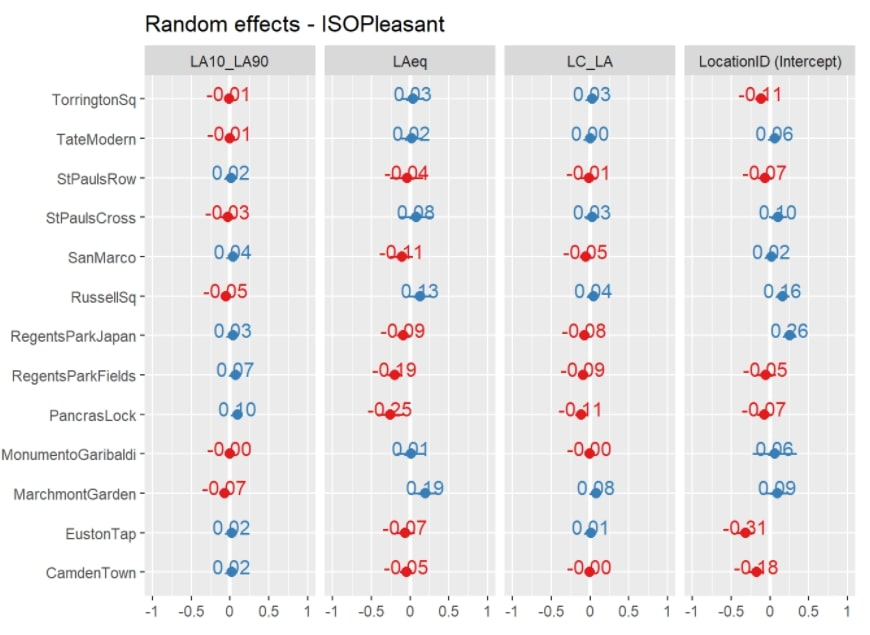
\includegraphics[width=\textwidth]{Figures/Lockdown Figure4.jpg}
   \end{figure}

   \subsubsection{\gls{isoev} model selected}

   Through the group-level feature selection, all of the group-level coefficients, including the LocationID factor itself. Therefore the final \gls{isoev} model is a 'flat' multi-variate linear regression model, rather than a multi-level model. The \gls{isoev} is a linear combination of \gls{s}, \gls{fs}, \gls{tu}, \gls{laeq}, and \gls{lcla}. The training and testing \gls{mae} are very similar, indicating that the model is not over-fit to the training data ($MAE_{train}=0.233; MAE_{test}=0.231$). The model performs slightly worse than the \gls{isopl} at predicting the mean location responses, but still performs well ($R^2_{train}=0.873; R^2_{test}=0.715$).

   \subsubsection{Application to lockdown data}
   %FIXME: Figure out how to do sub-figure referencing
   Once the two models were built and assessed, they were then applied to the lockdown recording data in order to predict the new soundscape ISO coordinates. \cref{fig:circumplex-locations}(a) shows the pre-lockdown ISO coordinates for each location and \cref{fig:circumplex-locations}(b) shows how the soundscapes are predicted to have been assessed during the lockdown period. As in the model assessment process, the predicted responses are calculated for each recording individually, then the mean for each location is calculated and plotted on the circumplex.

   In 2019 the majority of locations in the dataset fall within the 'vibrant' quadrant of the circumplex, particularly those which are primarily dominated by human activity (e.g. SanMarco, TateModern). CamdenTown and EustonTap, which are both in general visually and acoustically dominated by traffic, are the only two to be rated as 'chaotic', while no locations are overall considered to be 'monotonous'. During the 2020 lockdown, there is a general positive move along the 'pleasant' dimension and a general negative move along the 'eventful' dimension, but several patterns of movement can be noted. These are investigated further in the Discussion section below.

   \begin{figure}[h!]
     \caption{Soundscape circumplex coordinates for (a) the mean \gls{isopl} and \gls{isoev} responses for each location; and (b) the mean predicted responses based on recordings made during the lockdown and the location's movement in the circumplex. \label{fig:circumplex-locations}}
     \centering
     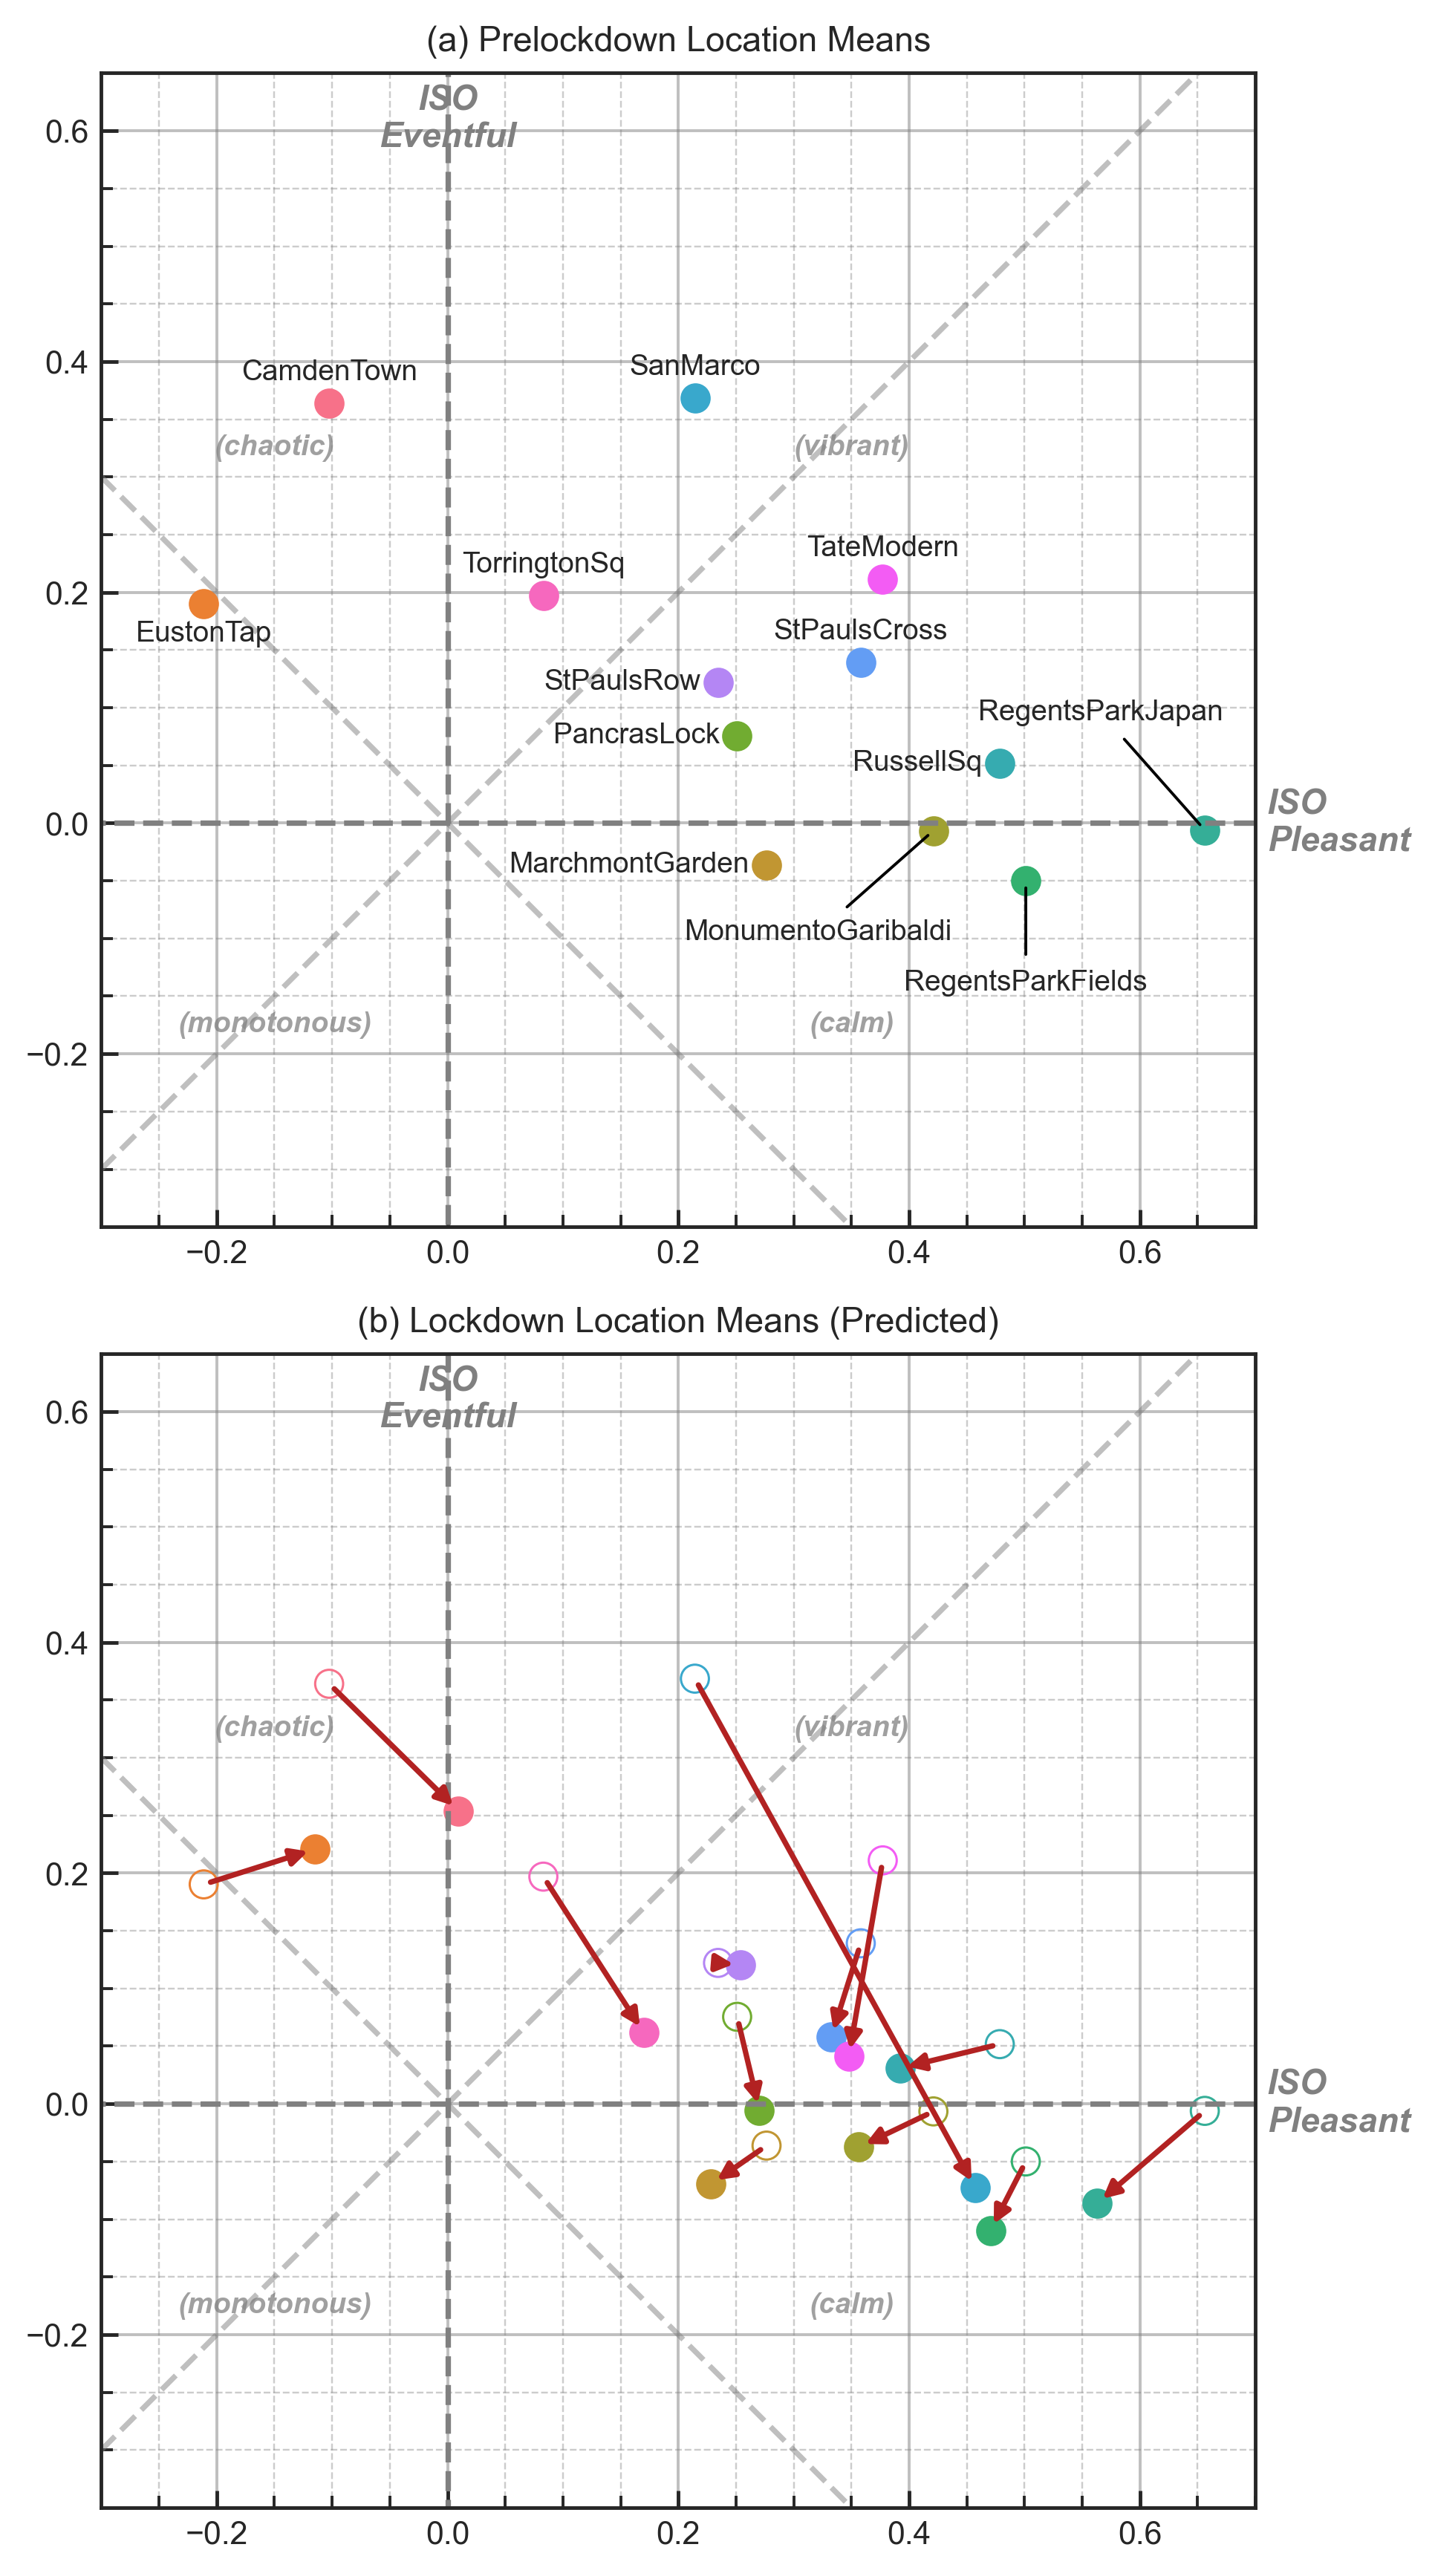
\includegraphics[width=.75\textwidth]{Figures/Lockdown Figure5.jpg}
   \end{figure}

   %%%%%%%%%%%%%%%%%%%%%%%%%%%%%%%%%%%%%%%%%%%%%%%%%%%%%%%%%%%

\section{Discussion}

 \subsection{Interpretation of the results}

   To interpret the results addressing RQ1 and RQ2, it is necessary to separately look into the overall change in sound source composition, and the change in the affective quality of soundscapes per location.

   \subsubsection{Change in the sound source composition}

   The open-ended question about sound sources in the online survey did not reveal a change in sound source types but rather confirmed that all types were still present in both conditions. The sound source composition question taken from the Method A of the ISO/TS 12913-2:2018 \citep{ISO12913Part2} revealed a statistically significant reduction in human sound sources and a significant increase in the perceived dominance of natural sound sources.

   The most frequent sound sources detected from the open-ended question correspond to the main four sound source types investigated, which indicated that all types remained present in the lockdown condition (at all the locations). While traffic intensity might have gone down, where the results of the Mann-Whitney U-test were inconclusive, but supported by the psychoacoustic measurements according to \citet{Aletta2020Assessing}, traffic-related sound sources were still clearly present.

   The sound source composition of an outdoor acoustic environment is extremely complex. Removing one component, such as human sounds, has implications on the whole \citep{Gordo2021Rapid}. Testing the effects of this in-situ is not straightforward and interpreting this study in line with 'what is the impact of human sounds' must be taken within the broader context of the range of conditions which changed within the acoustic environment. However, looking at the overarching picture, the lockdown condition was a useful and unique case study to understand the impact which human activities -- and the human sound source type in particular -- can have on soundscape perception of urban open spaces.

   \subsubsection{Movement of soundscapes}

   In order to interpret how the change of the acoustic environment at the locations examined would have been perceived, and to answer RQ2, movement vectors within the circumplex space are shown in \cref{fig:circumplex-vectors}. This clearly shows a few different patterns of movement due to the effects of the 2020 lockdown. These can be further looked into depending:

   \begin{enumerate}
     \item the magnitude of change,
     \item the direction of change,
     \item shift between the quadrants shown in \cref{fig:circumplex-locations},
     \item sound source composition.
   \end{enumerate}

   \begin{figure}[h!]
     \caption{The relative movement of soundscape perception in the circumplex due to the \gls{covid19} lockdowns, represented as vectors centred on the origin. *The lawn-works dominated session is shown separately as MonumentoGaribaldi* with a grey arrow to indicate that this is distinct from the effects of the lockdown changes. \label{fig:circumplex-vectors}}
    \centering
    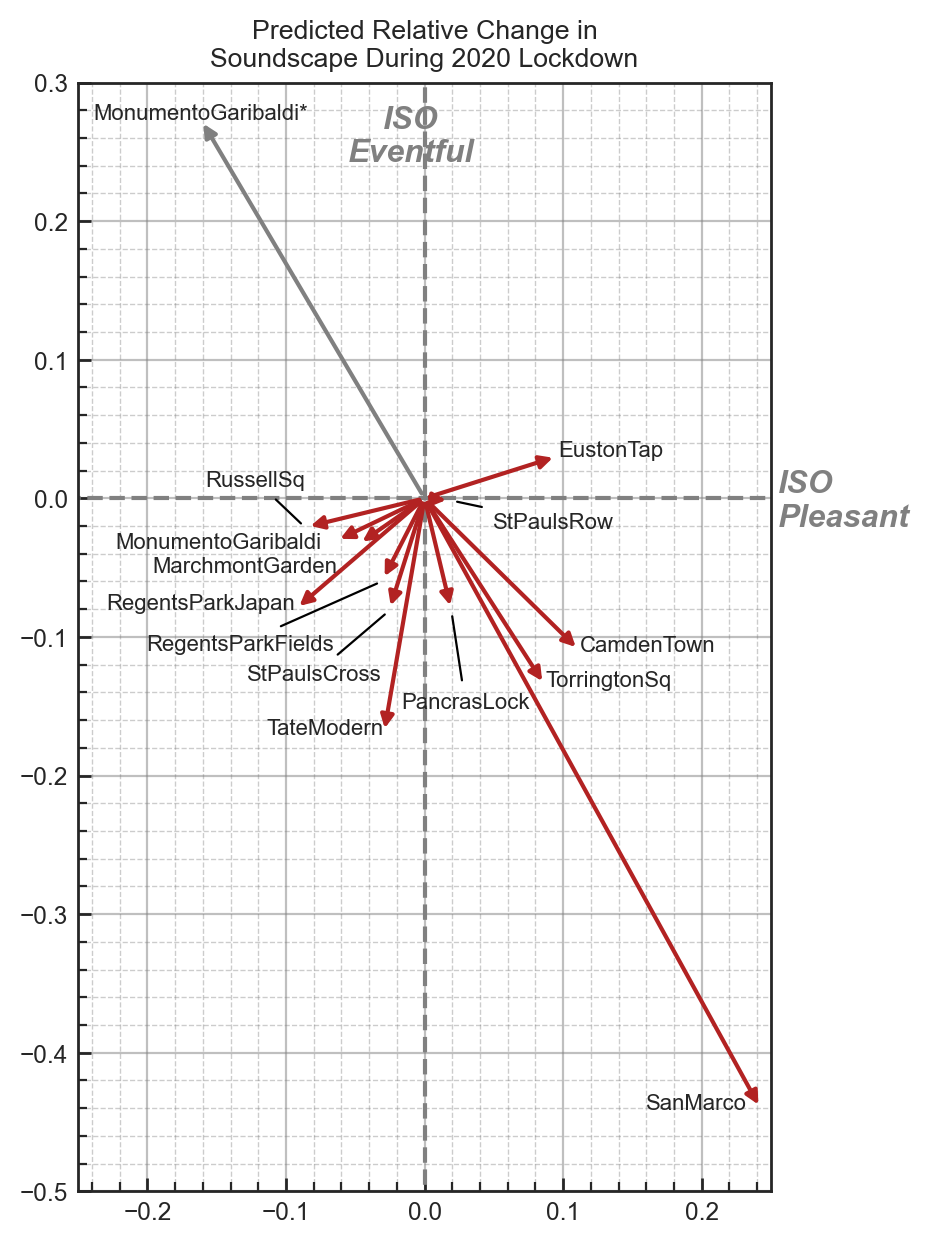
\includegraphics[width=.75\textwidth]{Figures/Lockdown Figure6.jpg}
   \end{figure}

   \paragraph{SanMarco} The largest change is seen in Piazza San Marco, with a predicted increase in pleasantness of 0.24 and a decrease in eventfulness of 0.44, enough to move the soundscape out of the 'vibrant' quadrant and into 'calm'. This extreme change (relative to the rest of the locations) is exactly what would be expected given the unique context of the measurements taken in 2019 -- the measurement campaign corresponded with Carnevale, a yearly festival which centres around the square. By contrast, due to the particularly strict measures imposed in Italy, during the lockdown measurement period the square was almost entirely devoid of people. What is promising is that, without any of this contextual information about the presence or absence of people, our model is able to capture and reflect what may be considered a reasonable and expected direction and scale of movement within the soundscape circumplex.

   \paragraph{EustonTap, CamdenTown, TorringtonSq, PancrasLock} The next locations of interest are those which, in the 2019 survey data, were rated as being dominated by traffic noise: EustonTap, CamdenTown, TorringtonSq, and PancrasLock. These are the only locations (besides SanMarco) which show a predicted increase in pleasantness. Of these traffic-dominated spaces, the two which were most heavily dominated by traffic noise (CamdenTown and EustonTap) showed the most increase in pleasantness, with TorringtonSq having slightly less of an increase. PancrasLock, which was also rated as having high levels of both Human and Natural sounds shows only a modest improvement in pleasantness.

   \paragraph{StPaulsCross, TateModern, RegentsParkJapan, RegentsParkFields, RussellSq} Among the locations which are predicted to experience a negative effect on pleasantness we see a mix of spaces which were assessed as being dominated by Human (StPaulsCross and TateModern) and Natural (RegentsParkJapan, RegentsParkFields, RussellSq) sounds before the lockdown. It is hard to discern a pattern of difference between these two groups, although it appears that the Human-dominated spaces saw a greater reduction in eventfulness, compared to the Natural-dominated spaces.

   In general, we note that most of the spaces experience some degree of reduction in eventfulness. This pattern is particularly consistent with what would be expected from a reduction in human presence in these spaces \citep{Aletta2018Towards}, as reflected by the observation that, in general, those spaces which had the most human sounds prior to the lockdown showed the greatest reduction in eventfulness during the lockdown.

   \paragraph{EustonTap} An unexpected result is that EustonTap is predicted to experience an increase in eventfulness and it is unclear whether this accurately reflects the real experience people would have had in the space. Normally, EustonTap is a mostly-outdoor drinking venue located at the entrance to the Euston Train station and is situated directly along a very busy central London road. During the 2020 survey, the researchers noted that the music and chatter of people from the pub was noticeably missing, but that the perceived reduction in road traffic was minimal. Based on the theory of vibrancy which would suggest it is driven by human presence and sounds \citep{Aletta2018Towards}, we would not therefore expect a shift in the vibrant direction as indicated here. This discrepancy may reveal a weakness in the context-independent \gls{isoev} model, or it may in fact be indicating that, at certain thresholds of traffic noise, a reduction in level -- and therefore a reduction in energetic masking -- will allow other aspects of the sound to influence the perception.

   \paragraph{MonumentoGaribaldi} Finally, special attention should be paid to the results shown for Monumento Garibaldi, which in 2019 was perceived as a pleasant and slightly calm green space featuring a gravel walkway. During the first measurement session during the lockdown in 2020, the researcher noted that the soundscape was dominated by landscaping works, in particular noise from strimmers (or weed whackers). In order to gain a sample which was more representative of the impact of the lockdowns, the researcher returned another day to repeat the measurements without interference from the works.

   To examine the impact of these two scenarios separately, the prediction model was fitted to the data from the two sessions independently and the session which was impacted by the landscaping works is shown in \cref{fig:circumplex-vectors} in grey and labelled MonumentoGaribaldi*, while the unaffected session is shown in red. In the latter case, the predicted change in soundscape as a result of the lockdowns fits neatly into what would be expected can closely matches the predicted behaviour of similar locations in London (i.e. MarchmontGarden and RussellSq). On the other hand, the session which was dominated by noise from the strimmers is predicted to have become much more chaotic, with a decrease in pleasantness of 0.16 and an increase in eventfulness of 0.27. This indicates that, although the model has no contextual information about the type of sound and in fact the training data never included sounds from similar equipment, just based on the psychoacoustic features of the sound it is able to reasonably predicted the expected change in soundscape.

   \paragraph*{}As a whole, the primary impact of the 2020 lockdowns on the soundscapes in London and Venice was an overall decrease in eventfulness. With the exception of EustonTap, all of the sessions show some degree of reduction in eventfulness, reflecting the general decrease in sound levels and human sound sources across the locations. The impact of the lockdowns on pleasantness is more mixed and seems to be driven by the previous dominance of traffic noise in the space. However, it could also be noted that, while all locations experienced a reduction in sound level, those which are predicted to become more pleasant had an average \gls{laeq} above 60 dB in 2019. By contrast, the locations which were predicted to experience a decrease in pleasantness generally had sound levels below 60 dB(A) in 2019. This may indicate that reductions in sound level can improve pleasantness when the sound level exceeds some threshold of around 60 - 65 dB(A) but are ineffective when sound levels are below this threshold. Similarly, \citet{Yang2005Acoustic} showed that, when the sound level is 'lower than a certain a certain value, say 70 dB' there is no longer a significant improvement in the evaluation of acoustic comfort as the sound level reduces. It is unclear at this point where this threshold would lie for pleasantness/annoyance, how strict it may be, or how it is impacted by the sound source composition of the acoustic environment, therefore further research is needed in this area.

   \subsubsection{Model selection results}

   The most immediately interesting result of the model-building and feature selection process, answering to RQ3, is the apparent irrelevance of location context to the \gls{isoev} dimension. The multilevel model structure was chosen since the starting assumption was that soundscape perception is heavily influenced by contextual factors, such as expectations of the space and visual context \cit{add references}. For this modelling, these factors can be considered as location-level latent variables at least partially accounted for by the inclusion of the LocationID as the second-level factor. While this assumption certainly held true for \gls{isopl}, our results indicate that these types of contextual factors are not significant for \gls{isoev}, and do not affect the relationship between the acoustic features of the sound and the perception.

   In particular this result may herald a shift in modelling approach for soundscapes -- where previous methods, in both the soundscape and noise paradigms, have mostly focused on deriving acoustic models of annoyance (in other words have focussed on the \gls{isopl} dimension) perhaps they should instead consider the acoustic models as primarily describing the eventfulness dimension when considered in-situ. In addition this study takes the approach of modelling responses at an individual level in order to derive the soundscape assessment of the location. Rather than either attempting to represent the predicted response of an individual person -- which is less useful in this sort of practical application -- or to base the model on average metrics of the location, the goal is instead to characterise the location itself, through the aggregated predicted responses of individuals. The authors believe this modelling approach better addresses the practical goal of predictive soundscape modelling and reflects the structure of the data collection.

   %TODO: Expand on this concept for the thesis.

 \subsection{Limitations of the study}

   The onsite sampling method was initially not intended as the ultimate characterisation of a location's soundscape but rather as a tool for model development. Therefore, the change observed does not necessarily represent the ground truth about the site's soundscape, if such a thing exists. Further, the online listening tests took a relatively small but random sample from the available database and did not include any contextual information. This proved to be sufficient for the purpose of detecting a change in sound source composition, however, the relatively small sample of recordings included in the online study does limit how representative they are of the location's sound environment as a whole.

   The surveys and recordings taken represent only a snapshot of the soundscape or sound environment for a short period in time. This is a flaw in most soundscape sampling methods presented both in the literature and in ISO/TS 12913-2. To truly be said to characterise the soundscape of a space, long-term monitoring and survey methods will need to be developed in order to capture the changing environmental and contextual conditions in the space. Models of the sort presented here, which are based on measurable quantities, could prove to be useful in this sort of long-term monitoring as they could take continuous inputs from sensors and generate the likely soundscape assessment over time.

   Further, the lockdown condition is likely to cause distortions of the circumplex soundscape perception model. Therefore, it is important to acknowledge that all the predictions were made for the people with no experience of the pandemic and its psychological effects. Conceptually, this model captured the perceptual mapping (i.e. the relationship between the acoustic indicator inputs and the soundscape descriptor outputs) of people in 2019, but this perceptual mapping is likely to have been affected by the psychological and contextual impacts of the lockdown itself, independent of its changes on the sound environment. Future research might look into potential perception changes in the post-pandemic world.

   %%%%%%%%%%%%%%%%%%%%%%%%%%%%%%%%%%%%%%%%%%%%%%%%%%%%%%%%%%%%%%%%%%%%%%%%%%

\section{Conclusion}

 This study demonstrates an application of predictive modelling to the field of soundscape studies. The model building results reveal that, within this dataset, an approach based on psychoacoustics can achieve $R^2=0.85$ for predicting the pleasantness of locations and $R^2=0.715$ for predicting the eventfulness. A modelling-focussed method of this sort is a key component to the potential scalability of the soundscape approach to applications such as smart city sensing, urban planning, and cost-effective, sustainable design. To demonstrate the usefulness and feasibility of such an approach, we apply our predictive model to a unique case study in which traditional soundscape survey methods were impossible.

 By applying this predictive model to recordings collected during the 2020 lockdown, the change in perception of the urban soundscapes is revealed. In general, soundscapes became less eventful, and those locations which were previously dominated by traffic noise became more pleasant. By contrast, previously human- and natural-dominated locations are in fact predicted to become less pleasant despite the decrease in sound levels. Although the results are limited in that they present one snapshot of the soundscape of the spaces, the success of the model in responding to new and disturbing sound events demonstrates its potential usefulness in long-term monitoring of urban soundscapes.

 %TODO: Sort out appendix and supplementary material from lockdown paper.

\part{Towards a Generalisable and Probablistic Soundscape Model}
\chapter{The predictive soundscape model framework}
\label{ch:bayes}
% alt:A Bayesian Hierarchical Predictive Soundscape Model and a Proposed Soundscape Index
% alt: Probabilistic soundscape models including personal, contextual, environmental, and acoustic information

% \section{Introduction}
% \subsection{The problem with the pleasant-annoying paradigm}

% As made clear by their name, noise annoyance studies have focussed on the relationship between noise (or acoustic) features and the perceived annoyance, to varying degrees of success. Within the soundscape circumplex framework, annoyance is the negative side of the pleasantness dimension, forming the \nth{1} primary component of soundscape perception. This means that, along with pleasantness, annoyance is that perceptual attribute which is most readily perceived and plays the largest part in differentiating between the perception of different soundscapes. This fact therefore makes this pleasantness dimension the prime target for addressing noise issues.

% However, \citet{Mitchell2021Investigating} (i.e. \cref{ch:lockdown}) and \citet{Aumond2022} have both recently demonstrated a fundamental difference in the statistical relationships connecting context and acoustic features with the perceived pleasantness and eventfulness of urban soundscapes. %TODO: Continue this discussion about including eventfulness. Can draw from that review I wrote



\section{Goals}
Before defining what form a general practical predictive model should take, we first need to make clear what the goals of such a model is. First, that it to a reasonable extent is successful in predicting the collective perception of a soundscape. As described in detail in \cref{ch:ProbabilisticPOC}, it should succeed at both indicating the central tendency of the soundscape perception, but importantly it should also inform the likely spread of perception among the population. The outcome of the predictive model should not be focussed on predicting an individual assessment; the goal is not to predict the perception of any specific individual, but to reflect the public's perception of a public space. In other words, ideally the model will result in an accurate distribution of soundscape perceptions for the target population. 

Second, that it can be implemented automatically. Once an initial setup is performed, such as identifying what location the measurements are conducted in, the model should be capable of moving from recorded information to predicted soundscape distribution without human intervention. We need soundscape to be able to be performed instrumentally. This enables it to be applied to unmanned uses, such as smart city sensors and soundscape mapping. It is impractical to conduct soundscape surveys or soundwalks in every location we wish to map and certainly not when we wish to see how these locations change over longer periods of time. A predictive model should allow us to survey these soundscapes remotely in order to extend soundscape to city-scale assessments. 

Third, the model should enable us to test and score proposed interventions. In a design context, it is crucial that various design strategies and interventions can be tested and that the influencing factors can be identified. The model should assist the user in highlighting what factor is limiting the success of a soundscape, spark ideas for how to address it, and allow these ideas to be tested. Several other useful features of predictive soundscape models arise out of these goals and will be discussed later, but these form the core goals of the framework.

\section{Constraints}
\label{sec:modelConstraints}
If we accept that predictive models are necessary to advance a more holistic approach to urban sound in smart cities, we must then define the constraints of such a model. The goal here is to define a framework for what is needed from a future model intended to be used in a smart city sensors, soundscape mapping, or urban design context.

The first constraint is that the model must be based on measurable factors. By this, I mean the data which eventually feeds into the predictive model should be collected via sensor measurements of one sort or another; this could be acoustic sound level measurements or recordings, environmental measurements, video recordings, or GIS measurements, etc.. What it certainly cannot include is perceptual data. This is strictly a practical constraint - for a predictive model designed to be used in practice, there is no justification to include other perceptual factors derived from surveys but not whichever factor you desire to predict. If the goal is to predict soundscape pleasantness and it is necessary to survey people about the visual pleasantness, why not just also survey them about the soundscape pleasantness directly? Certainly this mix of perceptual data is useful in research and can elucidate the relationships between the sonic and visual environments, but it is not useful in a practical predictive context. Any results which arise from research combining this sort of perceptual information must eventually be translated into a component which can itself be measured or modelled.

The second constraint is that any analysis of the measured data can be done automatically, without human intervention. If the eventual goal is to deploy the model on continuously-running, unmanned sensor nodes or to enable practical large-scale measurements, the predictive model should be capable of operating with minimal human input. This means, for instance, that if the model includes information about the sound source, this identification of the source should be possible to do automatically (i.e. through environmental sound recognition). Towards this goal, and given the current practical limitations of environmental sound recognition, a model using a manually-labelled sound-source data is used in \cref{ch:mlmann} to investigate the future potential of sound-source aware prediction models.

The third constraint is for the model to be generalisable to new locations. Ideally, it will be generalisable to new and (to it) unfamiliar soundscape types, but the minimum requirement should be that it can be applied to new locations which are otherwise similar to those in the training data. This means that any factors which are used to characterise the context provided by the location should be distinguished from a simple label of the location and should instead be derived from measurements of the location. In practice this could be geographical or architectural characteristics of the space, a proposed use-case of the space, or consistent visual characteristics of the space such as the proportion of pavement to green elements. This is in contrast to the model created for \cref{ch:lockdown} which was constrained to be used only on those locations included in the training data since it made use of a location label.

For this third point, some aspects of the first and second constraints can be relaxed. Since this would only need to be defined once for a location, definitions such as the use case of the space could be defined by the person using the model. What is necessary is that the model and its component location-context factors can be set up ahead of time by the user, then the recording-level effects are able to be calculated automatically. In the MLM context this essentially amounts to choosing the appropriate location-level coefficients ahead of time then automatically calculating the features which are fed into those coefficients (per constraint 1 \& 2).

A potential constraint for some applications is related to computation time. Since one proposed application of a predictive soundscape model is to embed the model on a \gls{wasn} node, the model would then need to be able to run on relatively low-power hardware such as a Raspberry Pi with a reasonable latency. This would especially present an issue for a model which relies on the combination of several psychoacoustic features, such as that in \cref{ch:lockdown} since these features are computationally intensive to calculate and several of them may need to be computed for each time step of the model. Although this is a real practical concern that should be addressed in the future, for the sake of this initial definition of a general predictive model used across many applications, I have not considered this as a strict constraint. The model being developed here would primarily be intended to operate as an off-line design tool operating on standard desktop hardware and not necessarily requiring real-time calculations. In the case of a \gls{wasn}, a model of this sort could still be used by sending recording information from the node to a central computer for further computation and analysis. Further efficiency improvements and a specific algorithm for embedding on the node is left as a future development.

Finally, the model should be robust to missing components. If the original or full construction of the model depends on demographic information of the population using the space, in cases where this information is not available, it should be possible to omit it and still obtain a reasonable result. Here we may define potential `must-have’ and `optional’ factors. Given the amount of variance explained by the various factors explored in this thesis, in-depth acoustic information is a must-have, while demographic and personal factors are an optional factor where the trade-off of losing 3\% of the explained variance in eventfulness (as will be shown in \cref{ch:whostudy}) is accepted as reasonable. Based on the results of \cref{ch:lockdown}, it would appear that location-context is crucial for modelling the pleasantness, but not for modelling the eventfulness. In order to determine the must-have factors for characterising the location-context, more work will need to be done to determine the appropriate input factors and their relative importance. The first step of this is to bring the model in line with constraint 3.

\section{Expansions and advancements for future predictive models}

To illustrate how a model which fits this proposed framework could be developed, I will start with the model presented in \cref{ch:lockdown}. As it is, this model most obviously violates constraint 3 - it is not generalisable to new locations. Since the structure of the \gls{mlm} has the `LocationID' as the categorical feature used in the second level, any new data must be able to conform to one of the original 13 locations. Technically, it would be possible to select the location in the training data which is considered most similar to the new location and use the coefficients derived for it, but this is a poor design for a generalisable model. Therefore the first stage to generalise this starting point model would be to replace the location-label variable with a more general categorical description of the location-context.

\subsection{Incorporating architectural and visual information}

The simplest version of this replacement would be to sort the locations into a predefined architectural or landscape location type. \citet{Suligowski2021Quantity} presents a definition in which urban spaces can be classed as `green' (unsealed, permeable, biologically active areas), `blue' (water areas), or `grey' (human made, predominantly formed by sealed, impermeable, hard surfaces built from concrete or tarmac). Thus we could sort the 13 locations used in the model according to whether they would be classed as green, blue, or grey and reconstruct the multilevel model using these categories in place of the location labels. In this way, new locations could then be similarly identified and fed into the model.

However, this simplified method has a few potential drawbacks. The green-blue-grey classification likely would not capture a wide enough array of potential landscape or architectural types and therefore would limit the ability of the model to differentiate the varying relationships between the acoustic features and the soundscape perception. In addition, the green-grey-blue paradigm does not provide an indication of the visual quality of the space. Although it might be assumed that green spaces are visually pleasant and grey spaces less so, there would presumably be some spectrum of quality within each of these categories which may provide additional information for the prediction of soundscape quality.

An alternative method is to make use of the visual information about the locations which can be capture as part of the \gls{ssid} protocol. The most straightforward method for this is to make use of a clustering algorithm to analyse measured features of the spaces and sort a given location into one of several location types. From a visual analysis model such as the FaceLift model presented by \citet{Joglekar2020Facelift}, it is possible to extract elements such as the percent of visible sky (i.e. openness), the percent of greenness, and an overall visual quality rating from photos and videos taken in the space. By applying an unsupervised clustering algorithm to this visual data, many more categories of the architectural and visual characteristics of the space can be derived and measurements of new spaces can likewise be assigned to these categories.

With this method, we would then have a two-stage model, where the first stage is to measure the visual characteristics of the space and, using the clustering algorithm, sort it into one of the identified categories. This category would be assigned to all subsequent acoustic measurements taken in the space as they are fed into the \gls{mlm} to predict the likely soundscape assessment.

\subsection{Additional acoustic, psychoacoustic, and bioacoustic metrics}

Although the model presented in \cref{ch:lockdown} began its feature selection with a relatively wide array of potential psychoacoustic features, many aspects of the sound were not captured and many potential metrics were not included. This includes additional statistical breakdowns of the included features - for instance, \gls{la90} (as a measure of the background level), $N_{10} - N_{90}$, $L_{A,max}$ and $L_{A,min}$, etc. There are also a host of bioacoustic metrics which were not considered, such as those presented in \citet{Devos2016Soundecology}, including the Acoustic Complexity Index (ACI), Normalized Difference Soundscape Index (NDSI), Bioacoustic Index (BIO), and so on.

An important sonic feature which is underutilised is the temporal behaviour of the sound. A few metrics are able to capture some aspects of how the sound changes over time, such as \gls{fs} looking at amplitude modulations in the sub-audible range, but this is still limited. One approach to characterising the temporal structure of complex acoustic scenes is through $1/f$ analysis \citep{deCoensel20031f,deCoensel2006quiet,Yang2015Presence}.
%TODO: Return here-1/f

Future work on expanding the predictive model should begin by considering these additional metrics and exploring their potential as new and better-performing input features for predicting soundscape perception.

With this increased slate of potential input parameters, a more efficient feature selection method will need to be employed, compared to the stepwise feature selection used throughout this thesis. The multicollinearity between the candidate features, the increased training time, and the ratio between independent variables and sample size make it infeasible to apply a stepwise selection with a large number of candidate features. 

In addition to a more sophisticated analysis of the acoustic characteristics of the sound, addressing the semantic meaning which listeners attach to certain sources is an important advance in predicting soundscape perception. The next chapter presents how I have begun to address this goal using data collected via a \gls{wasn}.
\chapter{Towards incorporating sound source information}
\label{ch:mlmann}

% \section*{Abstract}

% \copied{The recent development and deployment of Wireless Acoustic Sensor Networks (WASN) present new ways to address urban acoustic challenges in a smart city context. A focus on improving quality of life forms the core of smart-city design paradigms and cannot be limited to simply measuring objective environmental factors, but should also consider the perceptual, psychological, and health impacts on citizens. This study therefore makes use of short (1 - 2.7s) recordings sourced from a WASN in Milan which were grouped into various environmental sound source types and given an annoyance rating via an online survey with $N=100$ participants. A multilevel psychoacoustic model was found to achieve an overall $R^2=0.64$ which incorporates Sharpness as a fixed effect regardless of the sound source type and Roughness, Impulsiveness, and Tonality as random effects whose coefficients vary depending on the sound source. These results present a promising step torward implementing an on-sensor annoyance model which incorporates psychoacoustic features and sound source type, and is ultimately not dependent on sound level.}

\section{Introduction}

\footnote{The content of this chapter was originally published as \citet{Orga2021Multilevel}, a collaborative work between myself from the SSID team at UCL and Dr Ferran Orga, a researcher at Grup de Recerca en Tecnologies M{\'e}dia, La Salle-URL. Dr Orga and I shared first authorship on this paper. Original data collection was performed by the team at La Salle-URL while the data analysis and modelling strategy was conceived by the team at UCL and implemented by me. Dr Orga and myself drafted the original manuscript, with my work focussing on the analysis method section, results, and discussion of the modelling results.} In \citet{Brown2009acoustic}, the author proposes that one of the underutilised concepts in making use of sound as a resource is the disaggregation of sound sources. He states that `the type of sound sources present is critical in judgements about outdoor sound quality'. The goal is to move away from the straightforward use of aggregate sound metrics, which attempt to summarise the sound environment as a whole, through various acoustic metrics. Given the various semantic meanings that listeners associate with certain sound sources, the annoyance elicited by particular sounds will vary as will the relationship between the acoustic features of that sound and the annoyance \citep{LafayInvestigating}.

Given the nature of the \gls{isd} as a large dataset containing hundreds of \emph{in-situ} recordings, identifying sound sources manually was impractical. In order to progress towards a sound-source aware model, I therefore partnered with researchers from the LIFE DYNAMAP project who had curated a set of labelled recordings selected from a \gls{wasn} installed in Milan (Italy). For this study, the DYNAMAP researchers asked more than 100 people to conduct three different perceptual tests through an online survey \citep{AlsinaPages2021Perceptual}. 

The perceptual tests were designed to measure the annoyance in people relating to different urban sounds and their characteristics \citep{LabairuTrenchs2018Noise,AlsinaPages2021Perceptual}, by means of short excerpts of raw acoustic audio obtained from the DYNAMAP project \citep{Sevillano2016DYNAMAP}. The audio excerpts which were most representative of the site were selected, using a wide range of sound types (sirens, airplanes, people talking, dogs barking, etc.) \citep{Alias2020Aggregate,Alias2020WASN}. Sound annoyance depends on the acoustic characterisation of each sample, and it is possible to classify the acoustic excerpts depending on their sound source characterisation, which can be the basis to ask participants about their perceptions. The psychoacoustic characterisation is based on the psychoacoustic measurements of loudness, sharpness, and others defined by \citet{PsychoacousticsfactsmodelsZwicker}.

Based on the data collected by the DYNAMAP team, I aim to determine the psychoacoustic parameters that have an effect in the individual annoyance scores, and how the relationships between these parameters and annoyance may vary according to the dominant sound source. For this reason, a multilevel psychoacoustic model is trained using the results of the \gls{mushra} test \citep{IRB2015Method}, focused on annoyance evaluation by the participants over several different types of sound. The results show that sound source identification provides valuable information for a predictive model and that sharpness is a primary predictor for annoyance which is independent of the sound source.

%%%%%%%%%%%%%%%%%%%%%%%%%%%%%%%%%%%%%%%%%%%%%%%%%%%%%%%%%%
%TODO: Move to Lit Review
% \section{State of the Art of Annoyance Evaluation and Modelling}
% \label{sec:mod}
% In this section I gather a short synthesis of the most relevant contributions of the state-of-the-art on which the design of the tests and the modelling of perceptual annoyance have been based.

% \subsection{Evaluation of Annoyance}
% Past literature has focussed on the evaluation of annoyance by means of the objective parameters related to sound and noise \cit{10}. However, in order to measure the perception -- the real annoyance experienced by people -- the investigation can be greatly improved by considering the degree of annoyance produced by different sounds \cit{24, 25, 26}. Following the recommendation of the International Committee for the Biological Effects of Noise (ICBEN), this evaluation should be done in a qualitative way, using a verbal scale; this can be translated into \emph{not at all, slightly, moderately, very} and \emph{extremely}, just to give a few examples. Also an 11-point scale -- also from an ICBEN recommendation -- can be used, where in this case, zero corresponds to \emph{not at all} and 10 corresponds to \emph{extremely disturbing}.

% Borrowing from the subjective assessment of audio quality, the MUSHRA method has been also used for the evaluation of annoyance in \cit{17, 18}. \gls{mushra} was described and designed by ITU-R under the recommendation ITU-R BS.1534-3 \cit{23}. This recommendation gives guidelines on listening tests and subjective assessment, as well as audio quality (among other applications), assuming that the best way to evaluate audio quality is by means of subjective listening.

% Listening tests can be conducted in a controlled scenario (e.g. in an anechoic chamber) thus allowing the organiser to have control over the setup and experimental design. Nevertheless, this approach is expensive and time consuming. Alternatively, online listening tests have been widely used in the perceptual evaluation of audio quality or speech synthesis systems, even resorting to crowdsourcing strategies \cit{29}. These tests can be run in parallel and anywhere, thereby reducing costs and allowing researchers to reach a wider audience \cit{30}. In addition, these tests have seen increased use in the wake of the \gls{covid19} pandemic and its subsequent lockdowns. The limited access to facilities and equipment restricted how socio-acoustic and laboratory studies could be conducted, leading to the development of new online data collection methods. Recommendations for conducting such studies were given by \draft{the Acoustical Society of America in \cit{that guidance site}}. %TODO: Expand on this bit?

% \subsection{Annoyance Prediction}
% \copied{After the design and execution of the perceptual tests, the resulting evaluation coming from participants are used to generate a model that can predict the annoyance value depending on the type and the parameters of the noise excerpt under study. One of the most representative examples of annoyance modelling is found in \cit{15}, where a model based on the hypothesis that annoyance is primarily determined by the detection of intruding sounds is presented. The model takes into account several measurable elements:}

% \begin{enumerate}
%   \item signal-to-noise ratio (SNR);
%   \item indoor background level;
%   \item the activity conducted by the listener, assuming that in the conducted tests, their main activity is not listening to events.
% \end{enumerate}

% \copied{The model is obtained from the results of a test evaluating annoyance and acoustic data from a field experiment in a natural setting.}

% Another reference model for annoyance prediction is found in \cit{16}, where the authors model and predict road traffic noise annoyance based on:
% \begin{enumerate}
%   \item noise perception;
%   \item noise exposure levels;
%   \item demographics.
% \end{enumerate}

% \copied{The authors apply machine-learning algorithms in order to conduct the prediction and measure error rates, which give them a good trade-off in the prediction of the traffic noise annoyance, with a strong dependence on subjective noise perception and predicted noise exposure levels.}

% A model of annoyance based on a combination of psychoacoustic metrics was proposed by \citet{PsychoacousticsfactsmodelsZwicker}. Generated from laboratory-collected data, this model attempts to provide a method to directly calculate the relative annoyance values of single-source sounds from the psychoacoustic Loudness, Roughness, Sharpness, and Fluctuation Strength. this model has also been further expanded upon to include a term for the Tonality of the sound \cit{31}. However, this model was developed based on laboratory studies of generated, simple sounds (i.e. not real recorded sounds) and does not take into account the semantic information associated with the real environmental sounds present in an urban environment.

% In \cit{32}, the authors led us to a better understanding of the transportation noise-annoyance response, in three different and relevant approximations:

% \begin{enumerate}
%   \item to unravel the factors that affect the annoyance response of people in reference to the mixed transportation noise;
%   \item to contrast the noise-annoyance dependence in situations where road traffic and railway noise dominate;
%   \item to detail the differences between those two using structural equation modelling.
% \end{enumerate}

% As expected, the results show that annoyance is largely determined by noise disturbance and the noisiness perceived by citizens. Finally, in \cit{33} an approach to develop a road traffic noise prediction model is presented, and it takes into account:

% \begin{enumerate}
%   \item social aspects
%   \item characteristics of traffic, and
%   \item urban development
% \end{enumerate}

% It is based on the creation of a local model, with a pilot in Istanbul (Turkey), which uses all the information gathered for the creation of the noise maps as an input, and provides annoyance levels prediction as an output, complementing the noise maps which provide no subjective indicator.

%%%%%%%%%%%%%%%%%%%%%%%%%%%%%%%%%%%%%%%%%%%%%%%%%%%%%%%%%%

\section{Methods}

% In this section, I detail the several methods applied in this experiment from the perceptual test design based on an urban sound dataset \cit{21} to the multilevel linear regression modelling applied to obtain the annoyance prediction.

\subsection{Dataset}
\label{sec:DYANAMAPDataset}
%NOTE: Read LIFE DYNAMAP papers and summarise dataset collection?
This study makes use of a dataset collected in collaboration with the LIFE DYNAMAP\footnote{The data collection (both the collection of the recordings and the online survey) was performed by the DYNAMAP team. To maintain consistency with the published version of this study and to provide the appropriate context, the text on data collection (\cref{sec:DYANAMAPDataset,sec:DYNAMAPTests}) has been reproduced verbatim from our study \citep{Orga2021Multilevel} and was initially drafted by Dr. Orga, the first author.} project conducted in Milan (Italy) \citep{Sevillano2016DYNAMAP,Alias2020WASN}. This project makes use of a \gls{wasn}, enabling the collection of data over a longer period of time than was possible with the \gls{ssid} protocol outlined in \cref{chap:protocol}. A \gls{wasn} enables a broader characterisation of the acoustic events present in a location, as recording conditions can be made consistent across the nodes and data can be retrieved at any time of the day.

The dataset used in this study has been obtained by homogeneously sampling several hours, in both weekday and weekend, with 24 sensors distributed along the urban District 9 of Milan \citep{AlsinaPages2018Detection}. After that, experts from the DYNAMAP development team labelled the acoustic events of the recordings manually to obtain a 151-h dataset \citep{Alias2020WASN}. Due to the nature of the project, this consisted in removing events not related to traffic noise from the noise map computation, events were grouped in \gls{rtn} that belongs to the 83.7\% of the total time of the dataset, and \gls{ane} with the 8.7\% of the total time. Another class was used to include overlapping and unidentified events: \gls{complx} with 7.6\% of the total time \citep{Alias2020Aggregate}. During the labelling process, the DYNAMAP developers found up to 26 types of anomalous events, which they decided to group in the following classes: airplane, alarm, bell, bike, bird, blind, brake, bus door, construction, dog, door, glass, horn, interference, music, people, rain, rubbish service, siren, squeak, step, thunder, tramway, train, trolley, wind, works (construction) \citep{Alias2017Description}.

The most common sound classes were picked to evaluate the relationship between the event measurements and the citizens' perception of annoyance. These selected events used in the study belong to the following 9 classes: airplane, bird, brake, construction, dog, door, horn, people, and siren \citep{Orga2017Impact}. As the selected events are the most common, those are the ones that contain the widest variety of recording conditions, including different sensor locations and recording hours \citep{LabairuTrenchs2018Noise}. The reason for that choice was two-fold:

\begin{enumerate}
  \item the availability of a wide range of examples of each type of sound to choose for the design of the tests, including the possibility of finding different samples that keep similar psychoacoustic values,
  \item the fact that the most common sounds are the most reasonable to evaluate with people, as they best summarise the character of the soundscape around each sensor.
\end{enumerate}
% Particularly rewrite this paragraph, it's a very different style
% \copied{The comparison between events was only carried out with sounds collected using the same sensor, in order to ensure the same recording conditions. For this reason, if the chosen events for the perceptive tests belong to a sensor or another, depends on the availability of the classes to be compared in each sensor. In all the cases, measures were taken to ensure that the sensor containing the events has enough variety of samples with various psychoacoustic parameters, to ensure a proper representation of each category. To satisfy these requirements, only data from four sensors have been used to make the comparisons, as they provide enough information to carry out the perceptual test, i.e. hb115, hb124, hb127, and hb133 \cit{20}. }
More details about the event selection process and the availability of the study sensors are detailed in \citep{LabairuTrenchs2018Noise}, and the time of each event in the sensors is depicted in \citep{AlsinaPages2021Perceptual}.

\subsection{Design of the Perceptual Tests}
\label{sec:DYNAMAPTests}
In order to assess the degree of annoyance produced by the aforementioned classes of sounds, an online test was conducted using the Web Audio Evaluation Tool \citep{Jillings2015Web}. Specifically, the \gls{mushra} test method \citep{IRB2015Method} -- which was originally designed for the evaluation of audio codecs -- has been adapted for this purpose. Participants were given a clear explanation of what they were going to be asked, including detailed instructions on the operation of the test. No training phase was therefore considered. A demographic survey was included at the beginning of the test for all 100 participants, asking for them to identify their age, gender, and a subjective rating of the participant's residential area (zr1 - very quiet, zr2 - quiet, zr3 - bit noisy, zr4 - noisy, zr5 - very noisy).

The second part of the test consists of five sets. Each set presents a group of short acoustic events with similar values of loudness and sharpness but from different classes, and recorded in the same sensor, in order to maintain the recording conditions and location of the sounds under comparison. For each set, the participants were asked to evaluate the annoyance produced by the presented recordings, ordering them in a $0-10$ scale, where zero corresponds to \emph{not at all} and 10 corresponds to \emph{extremely disturbing} following the ICBEN recommendation. The interface was customised including a colour scale to help the participants place the stimuli according to the degree of annoyance that they perceive. Each audio is represented with a green bar with a `play' icon on it and the recordings are sorted randomly along the \gls{mushra} scale (see Figure \ref{fig:mushra-test}). An audio recording is reproduced when the corresponding bar is clicked. The system ensures the participant listens to all the recordings and moves all the bars before they jump to the next set of recordings. The sets were presented in a random order to prevent learning biases. \gls{mushra} tests usually include hidden reference stimuli, which in audio or speech quality evaluation corresponds to the highest quality samples and that are used to remove outlier responses.Since stimuli pertaining to different classes are compared, no audio reference was included, thus avoiding biases towards a certain audio class. The participants were asked to take the test using headphones and to keep the same volume during all the tests, to maintain the same conditions throughout the entire testing process. One hundred participants undertook this test, 59 men and 41 women, with a mean age of 33. Participants were volunteers, mainly from the university and also gathered via social networks. The distribution according to residential area is the following: 9 in zr1, 37 in zr2, 35 in zr3, 18 in zr4, and 1 in zr5. The \gls{mushra} test allows us to:

\begin{enumerate}
  \item obtain an individual score of annoyance for each audio,
  \item carry out comparisons among the different types of events contained in a set.
\end{enumerate}

The detail of the stimuli included in each of the five sets of the test can be found in Table \ref{tab:sensor-stimuli}.

\begin{figure}
  \label{fig:mushra-test}
  \centering
  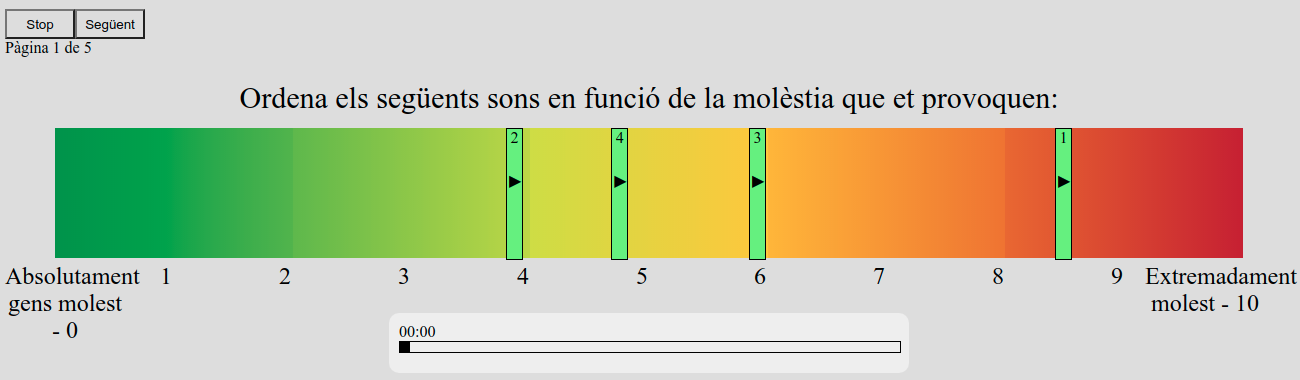
\includegraphics[width=\textwidth]{Figures/mushraScreenShot02.png}
  \caption{Screenshot of the \gls{mushra} test conducted to assess the annoyance provoked by different sounds. Title: sort the following sounds according to the cause annoyance. The scale ranges from \emph{not annoying at all} to \emph{extremely annoying}.}
\end{figure}

\subsection{Psychoacoustic Data Analysis}

The dataset resulted in 27 audio recordings of identified sound events with durations ranging between 1.01 and 2.69 s. The calibrated audio files were imported into the ArtemiS Suite software (v. 11.5, Head Acoustics GmbH) and the following psychoacoustic parameters were computed: \emph{loudness, sharpness, roughness, tonality} and \emph{impulsiveness} \citep{PsychoacousticsfactsmodelsZwicker}; values for these parameters are reported in Table \ref{tab:sensor-stimuli}. The rationale for selecting a relatively large set of psychoacoustic metrics is that they are often used as indicators to predict perceptual constructs (such as annoyance) in perceptual studies, as shown in recent soundscape literature \citep{Aletta2016Soundscape,Aletta2017Dimensions}. Fluctuation Strength, which could otherwise be included in this list of psychoacoustic parameters, as in Zwicker's annoyance model, was not included as the length of the recordings are too short to obtain a valid value. Loudness was calculated according to the DIN 45631 / A1 standard for time-varying sounds, in a free-field \citep{DIN2008Calculation}. As recommended by the standard, in order to avoid the under-estimation of evaluated loudness which is seen when using the arithmetic average of the loudness curve, the \gls{n5} value (the 5\% percentile value of the time-dependent loudness curve) is used as the single value of loudness. Sharpness was calculated according to \citet{DIN2009measurement}, in a free-field. With this sharpness method, the absolute loudness of the sound is not accounted for, so there should not be a duplication of information across the loudness and sharpness metrics. Roughness was calculated according to the hearing model by \citet{Sottek2017Sound}, with the option to skip the first 0.5 s in order to not distort the single value. Impulsiveness was also calculated according to the hearing model by Sottek, with a 0.5 s skip interval. Finally, tonality was calculated according to \citet{ECMA742019Measurement}, which is based on the hearing model of Sottek, with a frequency range of 20 Hz to 20 kHz.


\begin{table}
\centering
\caption{Psychoacoustic parameters calculated for the 27 stimuli used in the listening experiment. \label{tab:sensor-stimuli}}
\resizebox{\linewidth}{!}{%
\begin{tabular}{ccccccc} 
\toprule
\multirow{2}{*}{\textbf{Sensor }} & \multirow{2}{*}{\textbf{Label }} & \multicolumn{5}{c}{\textbf{Psychoacoustic Parameters }} \\ 
\cline{3-7}
 &  & \begin{tabular}[c]{@{}c@{}}\textbf{Loudness}\\\textbf{($N_5$ sone)}\end{tabular} & \begin{tabular}[c]{@{}c@{}}\textbf{Sharpness}\\\textbf{(acum)}\end{tabular} & \begin{tabular}[c]{@{}c@{}}\textbf{Roughness}\\\textbf{(asper)}\end{tabular} & \begin{tabular}[c]{@{}c@{}}\textbf{Tonality}\\\textbf{(tuHMS)}\end{tabular} & \begin{tabular}[c]{@{}c@{}}\textbf{Impulsiveness}\\\textbf{(iu)}\end{tabular} \\ 
\hline
hb133 & peop & 15.1 & 1.46 & 0.032 & 0.204 & 0.270 \\
hb133 & door & 16.8 & 1.43 & 0.029 & 0.113 & 0.354 \\
hb133 & dog & 13.1 & 1.22 & 0.033 & 0.373 & 0.266 \\
hb133 & brak & 16.0 & 1.76 & 0.030 & 0.326 & 0.241 \\
hb133 & bird & 12.6 & 1.73 & 0.024 & 0.283 & 0.214 \\
hb133 & airp & 13.0 & 1.27 & 0.060 & 0.438 & 0.231 \\ 
\hline
hb127 & sire & 17.7 & 1.56 & 0.045 & 1.540 & 0.178 \\
hb127 & peop & 16.1 & 1.62 & 0.035 & 0.410 & 0.417 \\
hb127 & horn & 18.1 & 1.56 & 0.028 & 0.666 & 0.260 \\
hb127 & door & 19.8 & 1.72 & 0.037 & 0.037 & 0.479 \\
hb127 & brak & 19.0 & 1.95 & 0.034 & 0.251 & 0.281 \\ 
\hline
hb127 & sire & 20.1 & 1.73 & 0.046 & 1.670 & 0.288 \\
hb127 & peop & 22.0 & 1.96 & 0.036 & 0.322 & 0.452 \\
hb127 & horn & 19.9 & 2.16 & 0.034 & 1.290 & 0.336 \\
hb127 & brak & 21.0 & 1.81 & 0.030 & 1.170 & 0.285 \\
hb127 & airp & 24.4 & 1.65 & 0.056 & 0.172 & 0.446 \\ 
\hline
hb115 & wrks & 20.3 & 1.97 & 0.054 & 0.227 & 0.267 \\
hb115 & trck & 24.4 & 1.60 & 0.033 & 0.040 & 0.276 \\
hb115 & sire & 19.5 & 1.46 & 0.054 & 0.861 & 0.333 \\
hb115 & peop & 25.1 & 1.79 & 0.032 & 0.411 & 0.331 \\
hb115 & horn & 22.3 & 2.00 & 0.032 & 0.806 & 0.155 \\
hb115 & door & 26.3 & 1.62 & 0.038 & 0.045 & 0.397 \\
hb115 & brak & 20.6 & 1.93 & 0.034 & 0.216 & 0.313 \\ 
\hline
hb115 & wrks & 24.6 & 1.92 & 0.064 & 0.447 & 0.317 \\
hb115 & sire & 26.6 & 1.77 & 0.044 & 0.626 & 0.290 \\
hb115 & horn & 29.5 & 2.35 & 0.039 & 0.486 & 0.262 \\
hb115 & door & 31.3 & 1.88 & 0.048 & 0.223 & 0.402 \\
\bottomrule
\end{tabular}
}
\end{table}

\subsection{Multi-Level Linear Regression Modelling}

The analysis for this study utilises a \gls{mlm}, with a random intercept and a random slope, using backward step feature selection. \glspl{mlm} are commonly used in psychological research for repeated measures studies \citep{Quene2004multi,VolpertEsmond2021Using} and for applied prediction models \citep{Gelman2006Multilevel,Frees2006Multilevel}. \gls{mlm} allows for the incorporation of nested and non-nested groups effects within the structure of the model, where the coefficients and intercepts for the independent variables are allowed to vary across groups. For this study, the data are grouped into two non-nested sets to form a two-level model: by repeated measures per respondent (\emph{user}) and by sound type (\emph{label}). In order to take into account the repeated measures across participants, and to correct for the participant's mean annoyance level, the \emph{user} variable is included in the second-level as a random intercept. We then include the psychoacoustic features as label effects, with coefficients which are allowed to vary across the sound type labels. The psychoacoustic features are also included as fixed effects in the first level, which do not vary across either the user or label groups.

The initial model structure, as written in Wilkinson-Rogers notation \citep{Wilkinson1973Symbolic}, is thus:

\begin{equation}
  % \begin{split}
  \label{eqn:initMLMann}
      Annoyance \sim N_5 + R + S + T + I + (1 | user) + (1 + N_5 + R + S + T + I | label)
  % \end{split}
  \end{equation}

\subsubsection{Feature Selection}

The \gls{mlm} is initially fitted with all of the potential features included within both levels. In order to reduce the complexity of the model, a backwards step features selection process is applied to both levels of the model. This process involves fitting the full model which includes all of the potential independent features (i.e. \cref{eqn:initMLMann}). The feature with the highest \emph{p}-value (least significant) is then removed from the candidates and the model is refit. This process is repeated until all features meet the predefined significance threshold of $p < 0.05 $. For a two-level model, first backward elimination of the second level is performed, followed by backward elimination of the first-level (or fixed) part.

If more than one feature is selected in the first-level, then the \gls{vif} is calculated in order to check for multicollinearity, with a pre-determined threshold of ${VIF}<5$. Any features which remain after the backwards stepwise selection and exceeded this threshold were investigated and removed if they were highly collinear with the other features. Once the feature selection process is completed, the final model with only significant features of interest included is fit and the table of the model coefficients is printed along with plots of the random effects and standardised estimates terms. Finally, quantile plots of the residuals and random effects are examined to confirm they are normally distributed \citep{Harrison2018brief}.

The input and output features are z-scaled prior to the analysis and model building by subtracting the mean and dividing by the standard deviation in order to directly compare the coefficient values of independent variables measured on different scales \citep{Harrison2018brief}. The model fitting and feature selection was performed using the \texttt{step} function from \texttt{lmerTest} (v. 3.1.3) \citep{Kuznetsova2017lmerTest} in the R statistical software (v. 4.0.5) \citep{RCT2018R}. The summaries and plots were created using the \texttt{sjPlot} package (v. 2.8.7) \citep{Luedecke2021sjPlot} and the multi-level $R^2$ values were calculated using \texttt{MuMIn} (v. 1.43.17) \citep{Barton2020MuMIN}.

%%%%%%%%%%%%%%%%%%%%%%%%%%%%%%%%%%%%%%%%%%%%%%%%%%%%%%%%%%%%%%%%%%%%%%%%%%%%%%%%

\section{Results}

\subsection{Differences in Annoyance between Groups \label{sec:groupDiffs}}
%NOTE: May remove this, it's Francesco's work

\footnote{The analysis carried out in \cref{sec:groupDiffs} was performed by Dr. Francesco Aletta. These results are included here verbatim from the original published paper to provide context for the later discussion on the influence of demographic differences on soundscape perception.}The average annoyance score of all users across all stimuli was $M=0.58 (SD=0.05)$. Since some basic demographic information about the 100 participants of the perceptual test was known, it seemed logical to explore possible differences in annoyance scores between different groups/levels of stratification of the sample, mostly for descriptive purposes. Therefore, Areas of residence and Gender were considered as factors in this analysis. Gender was treated as a binary variable (F/M), while Areas of residence was treated as a five-level categorical variable based on people's self-reported character of the area where they typically reside (range: 1-5; very quiet-very noisy). One-way repeated measures \gls{anova} was deemed to be the most appropriate approach to take into account the multiple responses that each of the 100 participants provided for the different recordings ($N=27$). A first analysis was then conducted to determine whether there was a statistically significant difference in annoyance between Areas of residence: no statistically significant differences were observed in this case $F(4.95)=1.374, p=0.249$. Likewise, a second one-way repeated measures \gls{anova} was carried out to check whether statistically significant differences in annoyance existed between females and males: no statistically significant effect was observed in this case either $F(1.98)=0.714, p=0.400$. Such small differences between groups can indeed be observed in Figure \ref{fig:anova}.

\begin{figure}[h]
  \label{fig:anova}
  \centering
  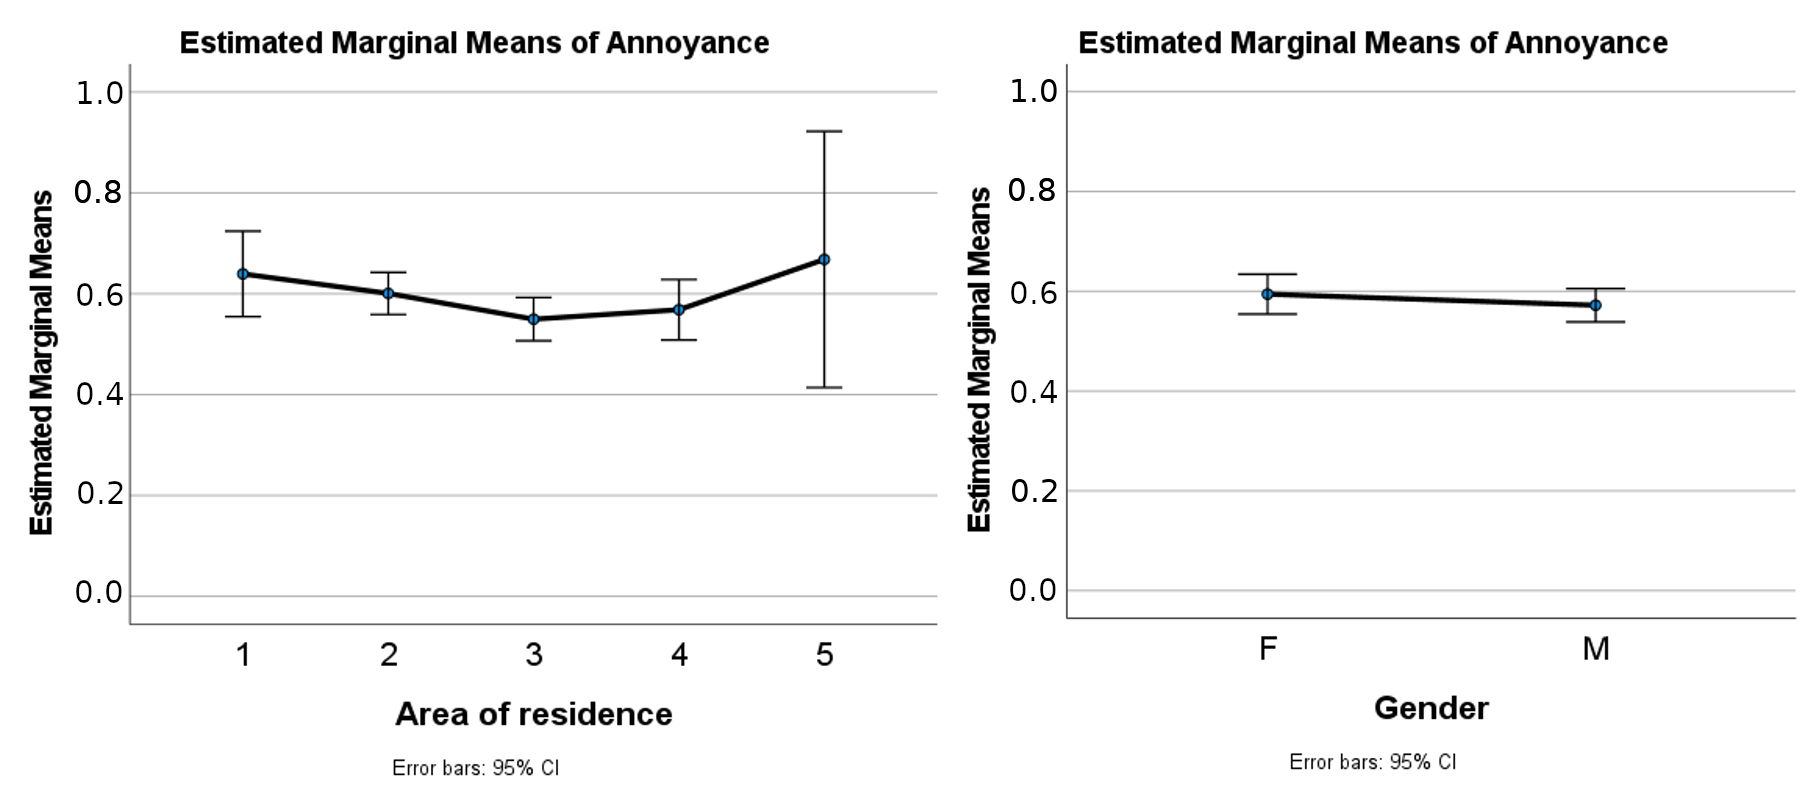
\includegraphics[width=\textwidth]{Figures/orga_anovas.png}
  \caption{Estimated Marginal Means for Annoyance as a function of Areas of residence (\textbf{left}) and Gender (\textbf{right}).}
\end{figure}

\subsection{Annoyance Model}
%TODO: Need to fix the ways I refer to the psychoacoustic features throughout the thesis. needs to be consistent
In the context of the multi-level linear regression modelling, the included variables were assumed to have an effect at two levels: the first level (i.e. fixed effect(s)), and the second level, where annoyance score intercepts are allowed to vary as a function of users (i.e. the 100 participants), and where each feature of interest is allowed its own coefficient as a function of labels (i.e. the 7 types of sounds). Sharpness came up as the main predictor with a strong statistical significance in the fixed-effect level, as reported in Table \ref{tab:annoyance-model}. This implies that, regardless of any other factors, the sharper the sounds, the more annoying they are perceived to be.

\begin{table}[h]
  \centering
  \caption{Random-intercept random-slope multi-level model of psychaocoustic annoyance, accounting for repeated measures (user) and sound source type (label) within the second level. Coefficients and confidence intervals given are for z-scaled data.}
  \label{tab:annoyance-model}
  \begin{tabular}{cccc} 
  \toprule
   & \multicolumn{3}{c}{\textbf{Annoyance }} \\ 
  \hline
  \textit{Predictors} & \textit{Estimates} & \textit{CI} & \textit{p} \\ 
  \hline
  (Intercept) & 0.02 & -0.13 -- 0.16 & 0.811 \\
  Sharpness & 0.33 & 0.25 -- 0.40 & \textbf{\textless{}0.001} \\ 
  \hline
  \textbf{Random Effects} &  &  &  \\ 
  \hline
  $\sigma^2$ & 0.47 &  &  \\
  $\tau_{00user}$ & 0.28 &  &  \\
  $\tau_{00label}$ & 0.02 &  &  \\
  ICC & 0.39 &  &  \\
  $N_{user}$ & 100 &  &  \\
  $N_{label}$ & 10 &  &  \\ 
  \hline
  Observations & 2700 &  &  \\
  Marginal $R^2$ / Conditional $R^2$ & 0.08 / 0.64 &  &  \\
  \bottomrule
  \end{tabular}
  \end{table}

The second-level effects presented in Figure \ref{fig:annoyance-effects} show that level- and loudness-based acoustic parameters do not play a significant role in predicting annoyance when considering other psychoacoustic factors and specific sound sources. However it should be noted that this may be influenced by the online data collection paradigm used in this study, which may struggle to control for the playback level. The variables selected by the feature selection algorithm within the type of sound (\emph{label}) level include: impulsiveness, roughness, tonality, and type of sound are relatively small, while roughness appears to be more important. For instance, when other effects are controlled, the sound type `horn' seems to be less annoying the rougher it is; while for the types of sound `bird' and `siren', higher roughness values will lead to higher annoyance scores. Looking at the model from the point of view of the types of sound, one could observe that `horns' tend to be more annoying than other sounds if they are more impulsive, while `people' or `birds' or `brakes' result in more annoying scores compared to other sounds if their tonal components are more prominent. Overall, for this model, the marginal and conditional $R^2$ values are 0.08 and 0.64, respectively. Marginal $R^2$ provides the variance explained by the fixed effects only, and conditional $R^2$ provides the variance explained by the whole model, i.e. both fixed effects and second-level effects. Thus, the majority of variance is explained by second-level factors, while a smaller portion (8\%) is covered by sharpness alone.

\begin{figure}[h]
  \label{fig:annoyance-effects}
  \centering
  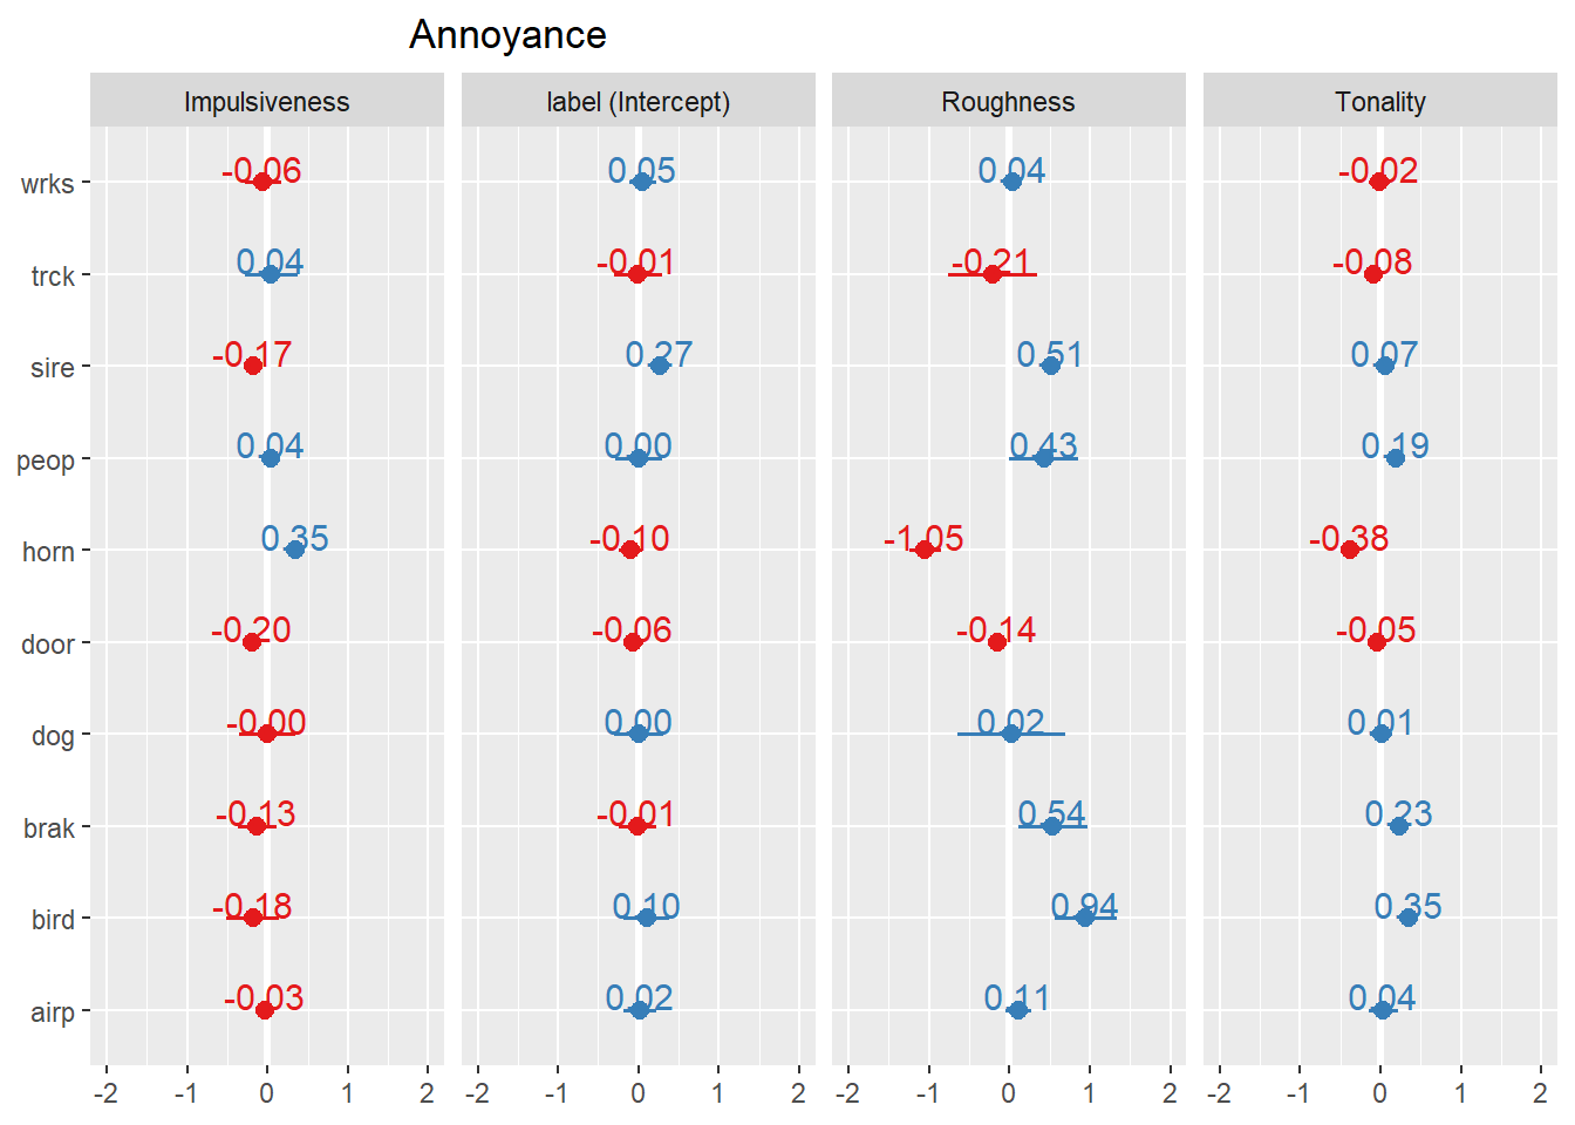
\includegraphics[width=\textwidth]{Figures/OrganMLMAnnoyanceRandom.png}
  \caption{Second-level effects figures representing the regression coefficients by types of sound (label) and for different psychoacoustic parameters.}
\end{figure}

%%%%%%%%%%%%%%%%%%%%%%%%%%%%%%%%%%%%%%%%%%%%%%%%%%%%%%%%%%%%%%%%%%%%%%%%%%%%%%%%%%%%%%%

\section{Discussion}

The fact that no significant differences in annoyance scores were observed between sample groups (i.e. gender or area of residence) is particularly interesting: it is common to assume in soundscape studies that personal and contextual factors play a strong role in how people respond to urban acoustic environments \citep{Kang2016Ten}. However, this is probably more relevant when complex sound environments (e.g. multi-source) are being considered and when dealing with relatively longer duration of exposures (e.g. several minutes) as seen in in-situ surveys. For clearly identifiable sources of environmental noise, with signals of short duration (i.e. 1-3s) like those used for this experiment, it is likely it was easier for the sample to converge on similar annoyance scores, regardless of other demographic factors. This aspect will be further investigated in \cref{ch:whostudy}.

Regarding the noise annoyance scores, sharpness came up as an important predictor in the first level of the modelling stage (explaining up to 8\% of the variance alone). It is important to highlight that the sharpness calculation method used in this study did not include any loudness correction; nor was any loudness-related parameter selected by the feature selection algorithm. To some extent, this is possibly due to the fact that, being an online experiment, it was not possible for the research team to actually calibrate the loudness playback level accurately for the remote participants. On the other hand, considering this aspect from the \gls{wasn} implementation perspective, this could be seen as an encouraging finding, since calibrating a diffuse acoustic monitoring network may not be practical in real-world scenarios, so it is good to have models that can achieve up to 64\% of variance explained regardless of actual levels. Furthermore, in complex acoustic environments, loudness would likely vary over time depending on the relative positions between sound sources and (human) listeners in ways in which the other psychoacoustic parameters such as sharpness and tonality are less likely to. This is something that is impossible for fixed sensors to take into account, so once again it is preferable not to rely on loudness as a predictor.

This result also appears to differ from some of the results in the model from \cref{ch:lockdown}, where sharpness was not selected as a final feature in the \gls{isopl} model. There are a few potential explanations for this. First, although within the circumplex pleasantness is considered the opposite of annoying, the respondents' annoyance rating in this study may be focussed on more specific or different factors than what is captured in the combined \gls{isopl} score. Second, since the \gls{isd} data is collected \emph{in-situ}, the general pleasantness of the soundscape may emphasise different acoustic features than the online study procedure used in this study. Finally, the structure of this model effectively controls for the influence of sound source information, whereas the \cref{ch:lockdown} model has no source information included. This could be interpreted as the sound-source-aware model more correctly identifying the acoustic feature which is important, independent of the sound source. Whereas the previous model's feature selection results may be more likely to select the features which help to differentiate sound sources, that is not necessary in the sound-source-aware model. This would indicate that the features selected in the \cref{ch:lockdown} model were selected because they perform better at differentiating sound sources and accounting for the semantic meaning associated with sound sources, but when the semantic information itself is included in the model, other acoustic features are more important for determining annoyance. 

Being able to predict noise annoyance from recorded sounds is particularly helpful from a public health perspective. In the context of a smart-city framework, one could imagine a \gls{wasn} large enough to cover a whole urban area; having a noise annoyance prediction algorithm at the node position that can return live annoyance scores to a central server from sounds recorded locally by the sensor would make for a useful application for environmental protection officers and other stakeholders at community or local authority level \citep{Kang2018Impact}. A relevant issue to consider from the \gls{wasn} perspective, is that in previous studies conducted in both urban \citep{Alias2020WASN} and \citep{Alias2020Aggregate} environments, a clear influence of the type of environment around the sensor location on the types of noise was seen. Not all urban and suburban locations around the sensors have frequent sirens or horns. The presence of these sounds depends on the most common activities (e.g. leisure, hospitals, etc.), the type of road (wide, narrow), and the type of buildings and houses surrounding the location. The types of sounds and their relative frequency of occurence can vary widely given the combination of these architectural and landscape characteristics. In the design of a general model for quality of life, the approach for considering sound source information presented in this chapter should be combined with the proposal for incorporating this architectural and contextual information developed previously in \cref{ch:bayes}.

% \subsection*{Positivity (or the absence of negativity?)}
% \draft{NEW!!}
% From the experience of the previous studies which are highly focused on the existing environmental acoustic and psychoacoustic metrics, one (of many) potential limitations has been revealed. For the most part, these metrics were designed to characterise various negative qualities of the sound. Certainly, they therefore have a negative correlation with positive assessments of the sound, but the simple fact is that they were conceived of and implemented in an attempt to quantify some sonic characteristic that was assumed by the researchers to contribute to a negative perception. Hence why in Zwicker's empirical formula for Psychoacoustic Annoyance \citep{PsychoacousticsfactsmodelsZwicker} $PA = N_5 (1 + \sqrt{\omega^2_S + \omega^2_{FR}})$, all of the constituent parts have positive coefficients.

% While this would not theoretically hinder a formula for describing positive aspects of the sound, it creates a sort of conceptual barrier. If all of these metrics are designed to capture negative aspects of the sound, then it is insufficient to use them create a formula to describe a positive sound, since that formula would only represent the 'absence of negativity', not necessarily positivity.

%TODO: Add a more indepth discussion and add a limitation  section to lead into DeLTA

%%%%%%%%%%%%%%%%%%%%%%%%%%%%%%%%%%%%%%%%%%%%%%%%%%%%%%%%%%%%%%%%%%%%%%%%%%%%%%%%%%%%%

%DONE: Restructure the Conclusion and Incorporating sections to be more cohesive with the rest of Part C
\section{Conclusions}

In this chapter, an online listening experiment was conducted with 100 participants to assess the noise annoyance induced by short recordings of individual environmental noise sources gathered via a wireless acoustic sensors network in Milan. The main conclusions of this study are:

\begin{itemize}
  \item The acoustic samples gathered from selected sensors in Milan \gls{wasn} of the DYNAMAP project led the DYNAMAP team to a structured \gls{mushra} test to evaluate the annoyance in an offline perceptual test.
  \item When considering short recordings of single-source environmental sounds, no significant differences in noise annoyance were observed as a function of demographic factors, such as gender and self-reported area of residence (i.e. from very quiet to very noisy).
  \item The multi-level linear regression model derived from this case study achieved an overall $R^2=0.64$, using sharpness as a fixed effect (the first level), and impulsiveness, roughness, and tonality as random effects allowed to vary according to the type of sound (the second level) as predictors for perceived noise annoyance.
\end{itemize}

%DONE: need ot rephrase this
% Taken together, the results of this study encourage us to continue our research work at all the stages described in this paper. The improvement of real-time algorithms to automatically detect the predefined sound sources under study is the first stage to gathering the most relevant samples in all and each of the sensors of a \gls{wasn}. The application of the annoyance modelling can give the \gls{wasn} a dimension without precedent: the availability of the objective acoustic measurements conducted by the sensors, and the estimation of annoyance in a real-time evaluation by means of the model. We can start to think about a dynamic annoyance map, which could be more far-reaching than a dynamic noise map.

\subsection{Incorporating into the general model}
Incorporating information about the sound source can greatly improve the prediction of perceived annoyance. The modelling structure used in this chapter effectively created separate, sound-source-dependent models of psychoacoustic annoyance, in contrast to the general annoyance model developed by \citet{PsychoacousticsfactsmodelsZwicker}. Each sound source (traffic, horns, people, etc.) has its own linear combination of psychoacoustic values to demonstrate how the semantic meaning which the listener assigns to a sound mitigates the perceptual mapping from physical inputs to perceptual outcomes. Incorporating this information, such that this semantic meaning influences the outcome of the ideal predictive model, is crucial. What is less clear is 1) how to deal with complex scenes where multiple overlapping sound sources are present and how to integrate this into the model; and 2) how this process can be automated, with minimal manual input from the model's users. %TODO: Expand on sound source inclusion

Given the somewhat unexpected result from this study that demographic factors had little difference on annoyance ratings, the next chapter will further investigate the influence of personal factors on soundscape perception making use of the larger and more diverse dataset from the \gls{isd}.
\chapter{Psychological Well-being and Demographic Factors can Mediate Soundscape Pleasantness and Eventfulness}
\label{ch:whostudy}
Soundscape studies aim to consider the holistic human perception of a sound environment, including both the physical phenomena and how these are mediated by internal factors. Within the context of the predictive modelling strategy presented in this thesis, the inclusion of personal factors presents a particular challenge. Referring back to our conceptual model of soundscape perception shown in \cref{fig:percepMap}, the form of the perceptual mapping which translates the soundscape indicators into a listener's perception (expressed via soundscape descriptors) is influenced by the listener's own psychological state and background. Although we can find general patterns in people's responses to soundscape indicators -- for instance, in general people have a strong annoyance reaction to roughness in sirens, but not in horns (see \cref{fig:annoyance-effects}, but this association may not have been formed for everyone equally) -- precisely how these responses are formed will differ from person to person. Our next step then, is to investigate to what extent people with similar demographic backgrounds, stages of development, or psychological states share a similar perceptual mapping. In short, we want to determine which personal factors influence the perceptual mapping and how much of the perceptual response can be explained by these factors.

The first step to exploring how we might account for the influence of personal factors is to establish which factors have the most influence and to what extent they can mitigate soundscape perception. Towards this, a first study was conducted on an early subset of the \gls{isd} data, making use of the demographic information (age, gender, educational status, ethnicity, and occupational status) and the psychological well-being included in the \gls{ssid} questionnaire.

\draft{The initial draft of the text of this study was written by the first author, Mercede Erfanian, based on our joint data collection and statistical modelling performed by me. This study underwent significant revisions following reviewers' comments and the later drafts of the manuscript, particularly the methodology and discussion sections, were written and revised by both Ms Erfanian and myself. Ms Erfanian's focus and expertise is on the psychological aspects of the work, so to maintain consistency with the published version, the background provided on the psychological theory and measures is reproduced verbatim. These sections will be explicitly noted where necessary. is to investigate to what extent the secondary factors mediate soundscape perception and to discuss how they may be incorporated into the predictive soundscape modelling framework.}
% \copied{Individuals with an aberrant psychological state and poor mental health may experience environmental inputs differently to those people who do not experience such issues given that emotions, as one of the core components of psychological well-being, and sensory perceptions are closely intertwined \citep{Kelley2014effects}. As reported in the relevant literature, the impact of psychological weell-being is consistent among all perceptual modalities such as vision \citep{Zadra2011Emotion}, tactile \citep{Kelley2014effects}, olfactory \citep{Krusemark2013When}, and auditory \citep{Riskind2014Influence}. In parallel, studies in the field of psychopathology edlucidated that individuals with poor psychological well-being, such as the clinically depressed, maintain bias and anomalous cognition, leading to inaccurate and distorted perception (Beck's cognitive theory) \citep{Clark2010Cognitive}.}

% \copied{The perception of the acoustic environment involves the sensation, identification, organisation, and interpretation of ongoing omnipresent auditory information \citep{Goldstein2014}. Soundscape perception does not always maintain consistency and shows a huge variation across individuals and, on a general scale, among populations \citep{Schneider2009Neural,Weinstein1978Individual}. There is evidence to suggest that the differences in the demographic characteristics like gender \citep{Gulian1986effects,Xiao2019Investigation}, age, and educational background \citep{Zhang2007Towards} may determine the way we perceive environmental sounds. Additionally, these individual differences can potentially reflect in various perceptual properties, implying the difference between the encoding of certain auditory information between individuals such as pitch \citep{Coffey2016Individual} or loudness \citep{Berthomieu2021Does}. However, the results from past studies have, for a good part, remained inconclusive or incosistent.}

\section{Introduction}

Whilst advancements have been made in understanding soundscape determinants, there is a lack of consensus in the literature about the impact of demographic factors on soundscape perception. Additionally, much work in this area relies on limited case studies \citep{Fang2021Soundscape,Ismail2014Sound,Yang2005Soundscape}. There is also a parallel set of literature examining the effect of psychological well-being on sound perception. However, as previous research in this area has typically focused on simple tones rather than complex sounds \citep{Laufer2016Behavioral,Riskind2014Influence}, controlled laboratory-based experiments, or subsets of individuals, the extent to which psychological well-being affects soundscape remains under-researched. Therefore, this study has two aims:

\begin{enumerate}
  \item to determine the associations between soundscape perception and demographic factors (i.e. age, gender, ethnicity, education level, occupation status);
  \item  to understand whether high levels of psychological well-being are associated with increased soundscape pleasantness and eventfulness
\end{enumerate}

To achieve this we explore the association between personal factors (including psychological well-being and demographics) and the soundscape perception using the \emph{in-situ} data collected in the \gls{isd}. In keeping with the methodology used throughout this thesis, this was investigated through a \gls{mlm}, which incorporates the LocationID as a proxy for contextual information in order to demonstrate what degree of explanatory power these personal factors may have for a predictive model. Finally, I discuss how these results should be considered in the context of my expanded predictive model and what methods may be used to include them as predictors.

% \copied{Whilst previous research has substantially advanced our knowledge of the soundscape determinants, past results are predominantly limited, often focussing on controlled laboratory-based experiments, individuals with psychopathology (i.e. depression) and investigating simple tones rather than complex sounds \citep{Laufer2016Behavioral,Riskind2014Influence}. In addition, the impact of psychological well-being in the context of soundsape, by its current definition, has still largely been unexplored. So, my first aim is to understand if high levels of psychological well-being are associated with increased soundscape pleasantness and eventfulness. }

% \copied{The second aim of the study was to determine the associations between soundscape perception and demographic factors, given there was insufficient consensus in the literature, and studies were restricted to limited case studies (i.e. Peace Gardens in Sheffield, UK) or a single ethnicity (i.e. Chinese) \citep{Fang2021Soundscape,Ismail2014Sound,Yang2005Soundscape}. I asked if age, gender, ethnicity, education level, and occupation status are associated with changes in the perceived soundscape pleasantness and eventfulness.}

% \copied{In this large-scale study, I explore the association of psychological well-being and demographic factors with soundscape perception among the members of the public with presumably no apparent psycholpathology in an immersive environment with diverse demographic characteristics such as ethnicity (i.e. American, Italian) and occupation status (i.e. student, retired).}

% \section*{Context}



% Linear mixed-effect modelling (i.e. multi-level modelling) applying backwards-step feature selection was used to model the interactions between the personal factors and the soundscape pleasantness and eventfulness, while accounting for the random effects of the survey location. This modelling method mirrors that used throughout the rest of this thesis and represents the development of my statistical approach, while focussing on a different aspect of the formation of soundscape perception.

% \section{Introduction}
%From Lit review:
% \copied{From a physiological point of view, a sound signal is a detectable change in our external environment that can elicit a series of unconscious responses, unbalancing our homeostastis (the dynamic state of equilibrium). These responses are similar among populations in a similar situation, are automatic, and regulated by the \gls{sns}. The \gls{psns}, on the contrary, is constantly active to maintain homeostastis. It has long been established that both the \gls{sns} and \gls{psns} are part of the \gls{ans}, which is \emph{per se} a division of the \gls{pns} \cit{8}. Humans and soundscapes have a dynamic bidirectional relationship -- while humans and their behaviour directly influence their soundscape, humans and their behaviour are in turn influenced by their soundscape. Several scientific communities in the area of neuroscience and psychology, therefore, have begun to pay close attention to our day-to-day exposure to particular sounds and their impact on the mental and physical health of individuals. Researchers in the areas of acoustics, environmental psychology, and auditory neuroscience outline the adverse impact of noise or negative sounds on well-being in an attempt to improve modern living standards \cit{20-24}. In this regard, ,evidence indicates that positively perceived sounds (e.g. natural sounds) are tied with a high quality of life and enhanced physiological and physical health \cit{5, 25-27}. Subsequently, \gls{art} argues the impact of nature (e.g. being exposed to natural sounds such as waterfalls) on humans improved cognitive performance and stress recovery \cit{28-31}. Not only has spending time in nature been demonstrated to have positive effects on humans' nervous system but it has also been shown that humans innately tend to seek connections with nature, a hypothesis known as Biophilia \cit{32}. These theories and effects demonstrate the effect external environments have on the health and well-being of individuals, but this relationship is bidirectional within the mind as well. The prior mental and psychological state of the individual will also influence how that individual experiences the environment and can change their perception of it.}

% \copied{The physiological and psychological approaches are two sides of the same coin in the realm of soundscape research, strongly interconnected and equally important. The psychological approach, in soundscape research, strives to depict the acoustic environment through the human behavioural pattern by borrowing a more deductive approach. It translates the underlying mechanisms into explicit behavioural manifestations, resulting from the perception of the acoustic environment. The physiological approach investigates the impact of the acoustic environment through the investigation of fundamental mechanisms of \gls{cns} and \gls{pns} by adopting a more inductive inferential approach. The physiological approach delineates the causation of the particular behaviour evoked by the environmental sounds.}

% \copied{The soundscape is composed of three main components -- human interaction, acoustic environment, and perception -- so it potentially draws attention across several life-science disciplines such as environmental psychology and public health, psychophysiology, and auditory neuroscience. To the best of the author's knowledge, no work previous to this review has highlighted the explicit psychophysiological underpinnings of the soundscape. The review in this chapter is the first work that reflects the fundamental mechanisms of the soundscape rather than its behavioural expressions.}

% \subsection{Psychophysiological studies}

% \subsection{Pleasantness and eventfulness as key components of soundscape perception}
% \draft{Move the following to Methods 2 or to Lit Review}

% \copied{Understanding the soundscape concept and its components largely depends on understanding the circumplex model of affect, proposed by James Russell \citep{Russell1980circumplex}. The circumplex model delineates the entanglement of the emotions and their neural substrates, opposing the classical model of discrete basic emotions \citep{Panksepp2004,Tomkins1962}. This model suggests that all affective states, described with descriptors such as alert, tense, or serene, arise from cognitive interpretations of core physiological and neural sensations. These affective states are produced by two fundamental neurophysiological systems, including two orthogonal continuums: valence and arousal, which can be discerned as a linear combination or as fluctuating degrees of activation \citep{Posner2005circumplex}.}

% Valence refers to whether an emotion is experienced as pleasant/positive or unpleasant/negative and is distributed horizontally on the circumplex space (on the X-axis). Arousal refers to whether an emotion is physiologically activating (high arousal; e.g. excited) or deactivating (low arousal; e.g. calm) (on the Y-axis) \citep{Russell1980circumplex}. High arousal is associated with activation of the sympathetic components of the \gls{ans} (e.g. increased heart rate) whereas low arousal is attributed to parasympathetic activation (e.g. slower heart rate).

% Similarly, the soundscape circumplex entails two main perceptual attributes: pleasantness and eventfulness which are different from the physical properties of the acoustic environment and by which the listeners appraise the quality of sounds \citep{ISO12913Part2}. Soundscape pleasantness refers to the emotional magnitude of the sound perception, while soundscape eventfulness is attributed to the intensity of the sound perception \citep{Erfanian2019Psychophysiological}. Like Russell's model structure the common model of representing soundscape is a bi-dimensional circumplex model with pleasantness on the X-axis and eventfulness on the Y-axis, proposed by \citet{Axelsson2010principal}.

% In their study, three primary dimensions of soundscape perception were extracted from participants' responses to complex sound samples measured on 116 attributes, using \gls{pca}. The first component was found to represent pleasantness (aligning with attributes such as comfortable, appealing, uncomfortable, disagreeable, and inviting) and explained 50\% of the variance in the dataset. The second component was found to represent eventfulness (eventful, lively, uneventful, full of life, and mobile) and explained 18\% of the variance. The third component was found to represent familiarity (commonplace, common, and familiar) and explained 6\% of the variance. In their final model, these attributes reduced to eight primary unidimensional scales of pleasant, vibrant, eventful, chaotic, annoying, monotonous, eventful, and calm and the reduced attributes can be further collapsed into two orthogonally positioned components of pleasantness and eventfulness (see 'Outcome variables').

% Likewise in this chapter, I employed the circumplex model reported in a two-dimensional scatter plot with coordinates for the two dimensions \gls{isopl} plotted on the X-axis and \gls{isoev} plotted on the Y-axis, taking into account the features of the locations. To differentiate these complex components from classic pleasantness and eventfulness in Axelsson's model, they are referred to as \gls{isopl} and \gls{isoev} throughout the text (see \cref{ch:circumplex} for further discussion on this process).

\section{Methods}

The study was approved by the local ethics committee of University College London (UCL), BSEER, Institute for Environmental Design \& Engineering (IEDE) (Dated 11-10-2019).

\subsection{Data Collection}
This chapter made use of a subset of data from the \gls{isd}. This study was conducted and published during the first round of \gls{ssid} data collection, prior to the first publication of the ISD. It includes 11 locations in London, with data collected from general members of the public. This chapter made use of the same \gls{ssid} questionnaire presented in full in \cref{app:questionnaire}, which is an adapted version of \citet{ISO12913Part2}\footnote{The ISO/TS 12913-2:2018 specifies requirements and provides supporting information on data collection and reporting for soundscape studies, investigations, and applications.} Method `A' (urban soundwalk method) and the WHO-5 Well-being Index \citep{Hall2011Examining}, as well as demographic information. As this chapter focusses on the items related to psychological well-being, demographics, and personal factors, we used a subset of the variables available in the full ISD. Only the sections of the questionnaire which were examined within this study are reported in this chapter. \cref{tab:whoDemo} reports the demographic characteristics of the sample used.


\begin{table}[!ht]
  \centering
  \caption{The sample demographic characteristics \label{tab:whoDemo}}
  % \resizebox{\textwidth}{!}{%
  \begin{tabular}{@{}ll@{}}
    \toprule
    Demographic characteristics                 & N(\%)                   \\ \midrule
    Total Samples                               & N = 1134                \\
    \textbf{Gender}                             &                         \\
    \quad Female                                & 610 (53.79)             \\
    \quad Male                                  & 524 (46.2)              \\
    \textbf{Age}                                &                         \\
    \quad Mean                                  & 34.67 years $\pm$ 15.11 \\
    \quad 18-30                                 & 627 (55.29)             \\
    \quad 31-40                                 & 195 (17.19)             \\
    \quad 41-50                                 & 112 (9.87)              \\
    \quad 51-60                                 & 97  (8.55)              \\
    \quad 61-70                                 & 72  (6.34)              \\
    \quad 71+                                   & 31  (2.73)              \\
    \textbf{Educational Level}                  &                         \\
    \quad Some high school                      & 22  (1.2)               \\
    \quad High school graduate                  & 315 (17.3)              \\
    \quad Trade/technical/vocational training   & 51  (2.8)               \\
    \quad University (undergraduate/bachelor)   & 422 (32.1)              \\
    \quad Postgraduate degree (master)          & 324 (17.8)              \\
    \textbf{Occupation Status}                  &                         \\
    \quad Employed                              & 613 (54.05)             \\
    \quad Unemployed                            & 25  (2.2)               \\
    \quad Retired                               & 84  (7.4)               \\
    \quad Student                               & 348 (30.6)              \\
    \quad Employed-Student                      & 5   (0.4)               \\
    \quad Other                                 & 44  (3.8)               \\
    \quad Rather not say                        & 15  (1.3)               \\
    \textbf{Ethnicity}                          &                         \\
    \quad White                                 & 806 (71.08)             \\
    \quad Mixed/Multiple ethnic groups          & 63  (3.5)               \\
    \quad Asian/Asian British                   & 156 (8.6)               \\
    \quad Black/African/Caribbean/Black British & 31  (1.7)               \\
    \quad Middle Eastern                        & 23  (1.3)               \\
    \quad Rather not say                        & 55  (3)                 \\
    \bottomrule
  \end{tabular}%
  % }
\end{table}

\subsubsection*{Psychological well-being/WHO-5 well-being index}
The \glsfirst{who5} is a validated metric used to quantify general well-being. It is measured by asking how individuals have been feeling over the last two weeks through a series of questions such as `I have felt cheerful and in good spirits'. The \gls{who5} has been designed for multiple research and clinical purposes, covering a wide range of mental health domains, namely perinatal mental health, geriatrics mental health, endocrinology, clinical, psychometrics, and psychiatric screening.

The \gls{who5} has been shown to be a coherent measure of well-being, with good validity \citep{Topp2015WHO}. For the purpose of analysis, a composite \gls{who5} score is calculated by summing the responses to each of the 5 questions (coded from 0 [for `at no time'] to 5 [for `all of the time']), then multiplying by 4 to get a single score which ranges from 0 (the lowest level of well-being) to 100 (the highest level of well-being) \citep{Topp2015WHO}. \citet{Blom2012Screening,LucasCarrasco2012Validity} have confirmed that the \gls{who5} items constitute an integrated scale in which items add up related information about the level of general psychological well-being among both young people and the elderly. 

% \copied{The \glsfirst{who5} asks how individuals have been feeling over the last two weeks such as `I have felt cheerful and in good spirits'. The \gls{who5} has been designed for multiple research and clinical purposes, covering a wide range of mental health domains, namely perinatal mental health, geriatrics mental health, endocrinology, clinical psychometrics, and psychiatric disorders screening.}

% \copied{The \gls{who5} is known to be one of the most valid generic scales for quantification of general well-being. In terms of the construct validity of the scale, \gls{who5} shoed to have properties that are a coherent measure of well-being \citep{Topp2015WHO}. With regards to relevant literature, \gls{who5} confirmed that all items constitute an integrated scale in which items add up related information about the level of general pscyhological well-being among both youngsters and elderlies \citep{Blom2012Screening,LucasCarrasco2012Validity}. For the purpose of analysis, a composite \gls{who5} score is calculated by summing the responses to each of the 5 questions (coded from 0 (for `at no time') to 5 (for `all of the time')), then multiplying by 4 to get a single score which ranges from 0 (the lowest level of well-being) to 100 ( the highest level of well-being) \citep{Topp2015WHO}.}

\subsubsection*{Demographic characteristics}
The demographic characteristics of each participant, including age, gender (male, female, non-conforming), education level (some high school, high school, trade/technical/vocational training, university, postgraduate), occupational status (employed, unemployed, retired, student, employed-student, other, rather not say), and ethnicity (Asian, Black/Caribbean, Middle Eastern, White, Mixed) were collected. Blank spaces were also provided if the participant wished to provide additional information. The demographic breakdown of the sample is presented in \cref{tab:whoDemo}.

\subsubsection*{Outcome variables (\gls{isopl} and \gls{isoev})}
\label{sec:whoOutcomeVar}
The outcome variables used for this study are the \gls{isopl} and \gls{isoev} coordinate values calculated according to Part 3 of \citet{ISO12913Part3}.

% \subsubsection*{Survey procedure}

% The data was collected according to the \gls{ssid} protocol outlined in \cref{chap:protocol}. The goal of the researchers on site was to collect a minimum of one hundred questionnaires from each selected site/location, which was typically achieved over a period of 2-3 days each consisting of approximately a 4 hour session. In some cases, either due to extenuating circumstances, time constraints, or excluded surveys, the full one hundred surveys were not achieved. The data for this chapter were collected from \nth{28} February 2019 to \nth{18} October 2019 between 11 a.m. and 3 p.m.

% In line with the \gls{ssid} protocol, during the survey period, acoustic and environmental metrics were simultaneously collected through binaural recordings, a calibrated \gls{slm}, and an environmental meter which recorded temperature, lighting level, and humidity data. The \gls{slm} was set up in the space in which the questionnaires were conducted (i.e. the \gls{environmental-unit}) and left running for the full duration of the survey in order to characterise the acoustic environment. The environmental metrics were not reported in this chapter since they were not in the scope of this study but are included in \cref{app:location-data} in order to provide context for the interested readers. 

\subsection{Data analysis strategy}

\subsubsection*{Data quality, missing data, checking for outliers, and data scaling}
In order to maintain data quality and exclude cases where respondents either clearly did not understand the \gls{paq} adjectives or intentionally misrepresented their answers, surveys for which the same response was given for every \gls{paq} (e.g. `Strongly agree' to all 8 attributes) were excluded. This is justified as no reasonable respondent who understood the questions would answer that they `strongly agree' that a soundscape is pleasant and annoying, calm and chaotic, etc. Cases where respondents answered `Neutral' to all \glspl{paq} are not excluded in this way, as a neutral response to all attributes is not necessarily contradictory. In addition, surveys were discarded as incomplete if more than 50\% of the \gls{paq} and sound source questions were not completed.


Prior to the data analysis, we imputed missing data and the imputed data was used across all analyses. Missing education values were imputed with the mode value (University). Missing values for age were imputed with the median age value (29). \gls{who5} (psychological well-being) missing values were imputed with the median value (64). We excluded those who responded `non-conforming' (N=4) or `decline' (N=21) for gender, due to the very small sample size and to simplify the effects of gender in the model. The initial data sample size was N=1467; the data included in the analysis N=1134.

We took a lenient approach to outliers. Due to the nature of survey data, it was typically inappropriate to remove data solely because it represented a deviation from the typical response. However, we wanted to catch data which was incorrect, intentionally wrong, or a typo and then remove them. For the most part, this was handled with my data quality method implemented in REDCap, to ensure the \gls{ssqp}/perceptual attribute values (N=8) were filled in such that they complied with the circumplex theory to a minimum degree. We were therefore, only looking for values which were extreme outliers or impossible.

\subsubsection*{Correlation between predictors and output variables}
To establish the relationships between all pairs of variables including the predictors and outcome variables, the Pearson correlation coefficient, \gls{anova}, and Chi-square were performed (as appropriate depending on whether the feature was continuous, ordinal, or nominal) between psychological well-being, age, gender, ethnicity, education level, occupation status, and the circumplex coordinate values (\gls{isopl} and \gls{isoev}). These results are given in \cref{tab:whoCorr}.

\subsection{Model specification (linear mixed-effects modelling)}

\glsfirst{lmer} with random intercept and fixed slope, using backward stepwise feature selection was utilised to (a) identify the association of the \glspl{foi} including psychological well-being, age, gender, education level, ethnicity, occupation status, and their interaction terms with \gls{isopl} and \gls{isoev} and (b) accommodate associations within participants among locations. In order to account for latent differences in the pleasantness and eventfulness ratings of various locations, the intercepts of each model are allowed to vary as a function of the location. Therefore, the model is constructed with two levels -- the individual level (the random effects) and the location level (the fixed effects). Separate models were constructed for each \gls{isopl} and \gls{isoev} and take the form:
%
\begin{equation}
  \label{eqn:whoPl}
  ISOPleasant_{ij} = \beta_{0j} + \beta_1 x_{1ij} + \beta_2 x_{2ij} + \ldots + \beta_n x_{nij} + \epsilon_{ij}
\end{equation}
%
\begin{equation}
  \label{eqn:whoEv}
  ISOEventful_{ij} = \beta_{0j} + \beta_1 x_{1ij} + \beta_2 x_{2ij} + \ldots + \beta_n x_{nij} + \epsilon_{ij}
\end{equation}
%
where $ISOPleasant_{ij}$ or $ISOEventful_{ij}$ are the dependent variable value for individual $i$ in Location $j$; $\beta_{0j}$ is the intercept for Location $j$; $\beta_1$ through $\beta_n$ are the slopes relating the independent variables $x_1$ through $x_n$ to the dependent variable; $x_{1ij}$ through $x_{nij}$ are the dependent variables for individual $i$ in Location $j$; $\epsilon_{ij}$ is the random error for individual $i$ in Location $j$. In turn, $\beta_{0j}$ can be expressed as:
%
\begin{equation}
  \beta_{0j} = \gamma_{00} + U_{0j}
\end{equation}
%
where $\gamma_{00}$ is the mean intercept across Locations; and $U_{0j}$ is the unique effect of Location $j$ on the intercept. In a random intercept model, the slope coefficients ($B_n$) are considered fixed across the locations (hence, labelled as the fixed effects) indicating that the relationship between the dependent variable (e.g. age, gender, etc.) and the independent variable (\gls{isopl} or \gls{isoev}) is the same for all locations, while the general \gls{isopl} of the location is accounted for by the varying intercept.

In order to identify the significant \glspl{foi} within the multi-level structure, I employed a stepwise feature selection on the fixed effects portion of the mixed-effects model, with an inclusion threshold of $p < 0.05$. Since this model includes only the LocationID at the random effects level, only the fixed effects are reduced in the feature selection process. To check for multicollinearity among the selected features, the \glsfirst{vif} was calculated and a threshold of $VIF < 5$ was set. Any features which remained after the backwards stepwise selection which exceeded this threshold were investigated and removed if they were highly collinear with the other features. Once the feature selection process is completed, the final model with only significant \glspl{foi} included is fit and the table of the model coefficients is printed along with plots of the random effects and z-scaled and non-standardised estimates terms.

The model fitting and feature selection was performed using `lme4' (version 1.1) and the `step' function from `lmerTest' (version 3.1.3) \citep{Kuznetsova2017lmerTest} in R statistical software (version 4.0.3) \citep{RCT2018R}. The summaries and plots were created using the `sjPlot' package (version 2.8.6) \citep{Luedecke2021sjPlot}.

\section[Results]{Results\footnote{This section closely resembles the Results section of the original paper \citep{Erfanian2021Psychological} of which I was the second author. I contributed significantly to the drafting of the original paper and in particular to the analysis and results presented here.}}

\subsection{Correlations}

\cref{tab:whoCorr} presents a matrix of the correlation coefficients for the features of interest. It should be noted that these correlations are calculated across the entire pooled sample, and therefore do not account for the multi-level structure of the LocationID. Age, education, gender (male), and \gls{who5} are all positively correlated with \gls{isopl}. However, only age is directly (negatively) correlated with \gls{isoev}. Age, education, and \gls{who5} are all similarly correlated with \gls{isopl}, while gender has a lower effect. It is worth noting that, while occupation is not directly correlated with either of the outcome variables, it is significantly correlated with all of the other independent variables considered in the study and highly correlated with age. As will be noted in the modelling results, this means it can act as a proxy for several of these other features in certain circumstances.

\begin{table}[!h]
  \centering
  \caption{Correlation coefficients for study variables. **$p<0.005$, *$p>0.05$\label{tab:whoCorr}}
  \begin{tabular}{@{}l|lllllll@{}}
    \toprule
    Factors     & Age              & Education       & Ethnicity       & Gender         & Occupation & WHO-5            & ISOPleasant      \\ \midrule
    Age         &                  &                 &                 &                &            &                  &                  \\
    Education   & 0.32             &                 &                 &                &            &                  &                  \\
    Ethnicity   & 0.23             & 0.04            &                 &                &            &                  &                  \\
    Gender      & \textbf{-0.1**}  & 0.05            & \textbf{0.08*}  &                &            &                  &                  \\
    Occupation  & \textbf{0.71**}  & \textbf{0.19**} & \textbf{0.13**} & \textbf{0.1*}  &            &                  &                  \\
    WHO-5       & \textbf{0.12**}  & 0.1             & \textbf{0.1*}   & 0.02           & 0.16       &                  &                  \\
    ISOPleasant & \textbf{0.13**}  & \textbf{0.12**} & 0.11            & \textbf{0.07*} & 0.16       & \textbf{0.14**}  &                  \\
    ISOEventful & \textbf{-0.08**} & 0.08            & 0.07            & 0.05           & 0.12       & 0.00             & \textbf{-0.24**}  \\ \bottomrule
  \end{tabular}
\end{table}

\subsection{Linear mixed-effects modelling}
\label{sec:whoLMERinit}
The linear mixed-effects regression derived regularised models of the soundscape pleasantness and eventfulness. This model was then reduced via backward stepwise feature selection. \cref{tab:whoLMER} presents the \gls{isopl} and \gls{isoev} models, including non-standardised and standardised estimate values and \glspl{ci} for the selected features that survived from the initial model. After the feature selection, age, education, and ethnicity were not found to be significant features in either the \gls{isopl} or \gls{isoev} models. It should be noted, however, that the presence of one feature (e.g. occupation) which is highly correlated with another (e.g. age and gender) may cause one of the features to not meet the threshold of significance when both are included, causing it to be removed during the stepwise feature selection. Nonetheless, it may be that, in a final model which included either of these features (but not both), they would each be considered significant. In this way, even though occupation was selected during this process, age may also have been considered significant, when not considering occupation. This behaviour is explored in more detail later.

\begin{table}
\centering
\caption{Fixed and random effects in a linear mixed model explaining variations in \gls{isopl} and \gls{isoev} while controlling for psychological well-being and demographic factors. The standardised estimates are calculated by refitting the model on standardised data scaled by subtracting the mean and dividing by 1 SD, allowing a comparison of all features. **$p<0.005$, *$p>0.05$  \label{tab:whoLMER}}
\label{tab:whoLMER}
\resizebox{\linewidth}{!}{%
\begin{tabular}{lccc|ccc} 
\toprule
 & \multicolumn{3}{c|}{\textbf{ISOPleasant}} & \multicolumn{3}{c}{\textbf{ISOEventful}} \\ 
\midrule
\textbf{Predictor} & \textbf{Estimates} & \textbf{Std. Est.} & \textbf{95\% CI} & \textbf{Estimates} & \textbf{Std. Est.} & \textbf{95\% CI} \\
WHO-5 & 0.001** & \textbf{0.03} & 0.01, 0.05 & 0.001 & 0.01 & -0.02, 0.04 \\
Gender (male) & - & - & - & \textbf{-0.08*} & \textbf{-0.04} & -0.07, -0.00 \\
Occupation         (Rather not say) & -0.19* & \textbf{-0.19} & -0.36, -0.02 & \textbf{0.7**} & \textbf{0.02} & -0.13, 0.17 \\
Occupation         (Retired) & 0.1** & 0.10 & 0.03, 0.18 & \textbf{-0.18**} & \textbf{-0.11} & -0.18, -0.04 \\
Occupation         (Unemployed) & 0.01 & 0.01 & -0.13, 0.14 & \textbf{0.01**} & \textbf{0.18} & 0.06, 0.3 \\
WHO-5 x Gender         (male) & - & - & - & \textbf{-0.001*} & \textbf{-0.04} & -0.07, -0.00 \\
WHO-5 x Occupation         (Rather not say) & - & - & - & \textbf{-0.01**} & \textbf{-0.21} & -0.33, -0.09 \\ 
\midrule
\multicolumn{7}{l}{\textbf{Random Effects}} \\ 
\midrule
$\sigma^2$ & \multicolumn{3}{l|}{0.11} & \multicolumn{3}{l}{0.08} \\
$\tau_00$ & \multicolumn{3}{l|}{0.06$_{Location}$} & \multicolumn{3}{l}{0.01$_{Location}$} \\
ICC & \multicolumn{3}{l|}{0.35} & \multicolumn{3}{l}{0.15} \\
N & \multicolumn{3}{l|}{11} & \multicolumn{3}{l}{11} \\ 
\midrule
Observations & \multicolumn{3}{l|}{1134} & \multicolumn{3}{l}{1134} \\
Marginal $R^2$/ Conditional $R^2$ & \multicolumn{3}{l|}{0.014 / 0.354} & \multicolumn{3}{l}{0.039 / 0.181} \\
AIC & \multicolumn{3}{l|}{779.125} & \multicolumn{3}{l}{451.351} \\
\bottomrule
\end{tabular}
}
\end{table}

\subsubsection*{Psychological well-being and its association with pleasantness and eventfulness}

The final models found that a higher level of psychological well-being and retirement are associated with higher pleasantness, while individuals that prefer not to report their occupational status showed a negative association with pleasantness. Further analysis revealed that psychological well-being was negatively associated with eventfulness in men and individuals that did not report their occupational status. Additionally, we detected that eventfulness is positively associated with unemployment, whereas it is negatively associated with gender (male) and retirement (\cref{tab:whoLMER}). 

The marginal and conditional $R^2$ values are given for each model in \cref{tab:whoLMER}. In a mixed effects model, the marginal $R^2$ represents the variance explained by the fixed effects (the individual-level independent variables) while the conditional $R^2$ represents the variance explained by both the fixed and random effects \citep{Nakagawa2012general}. From the conditional $R^2$, we can say that the full models explain 35.4\% and 18.1\% of the variance in \gls{isopl} and \gls{isoev}, respectively (\cref{fig:whoRand}). While the majority of the variance is explained by location-level differences (as confirmed by the \glspl{icc}), 1.4\% of variance in \gls{isopl} and 3.9\% of variance in \gls{isoev} is explained by the \glspl{foi} (i.e. psychological well-being and age) included as fixed effects.

%TODO: Recreate the random effects figures
\begin{figure}[!h]
  \centering

  \begin{minipage}{.5\textwidth}
    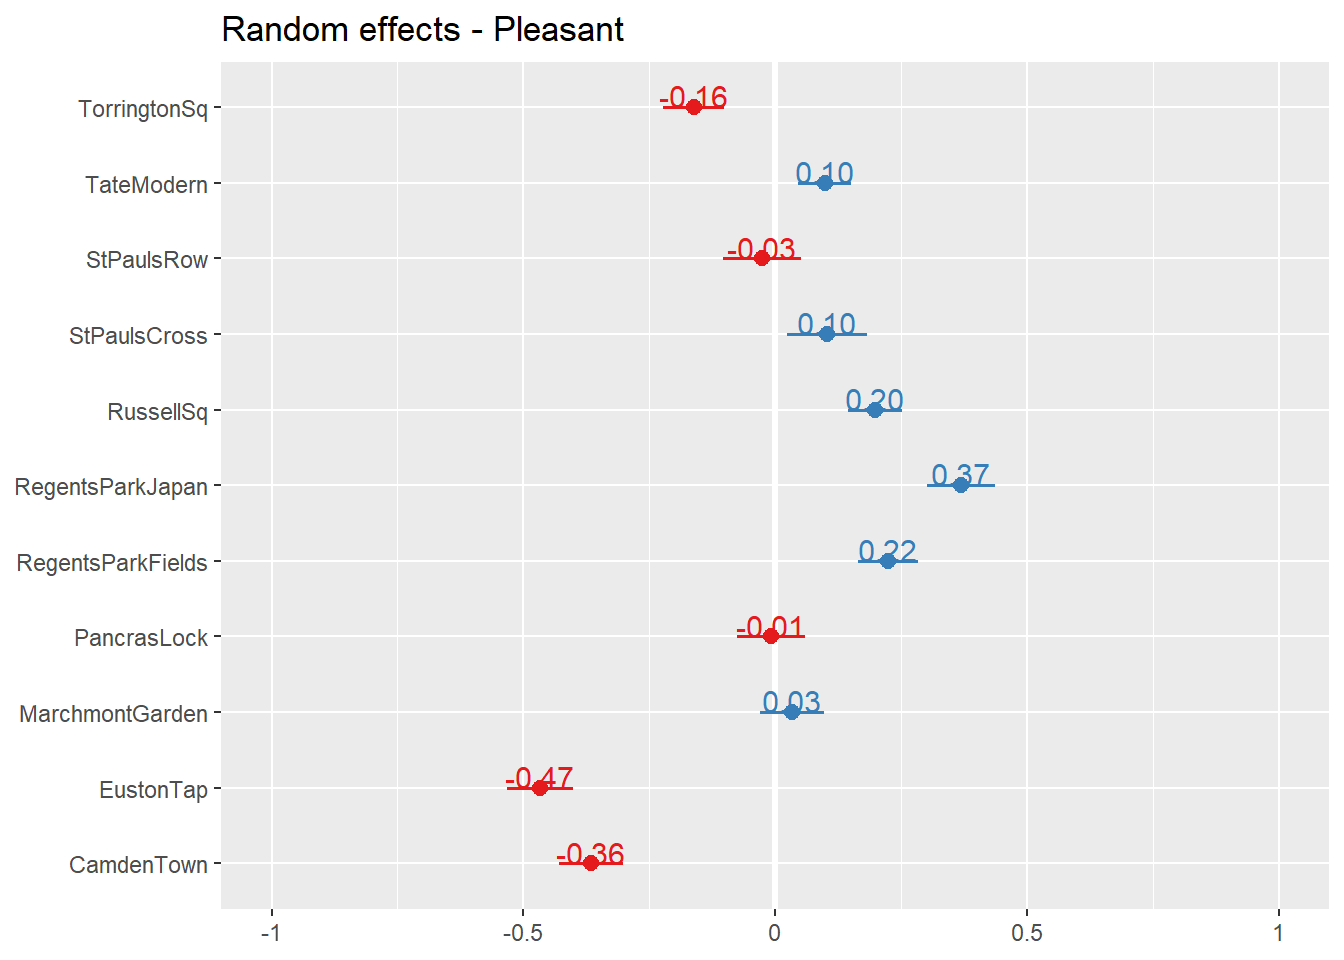
\includegraphics[width=\linewidth]{Figures/whoRandPlNew.png}
  \end{minipage}%
  \begin{minipage}{.5\textwidth}
    \centering
    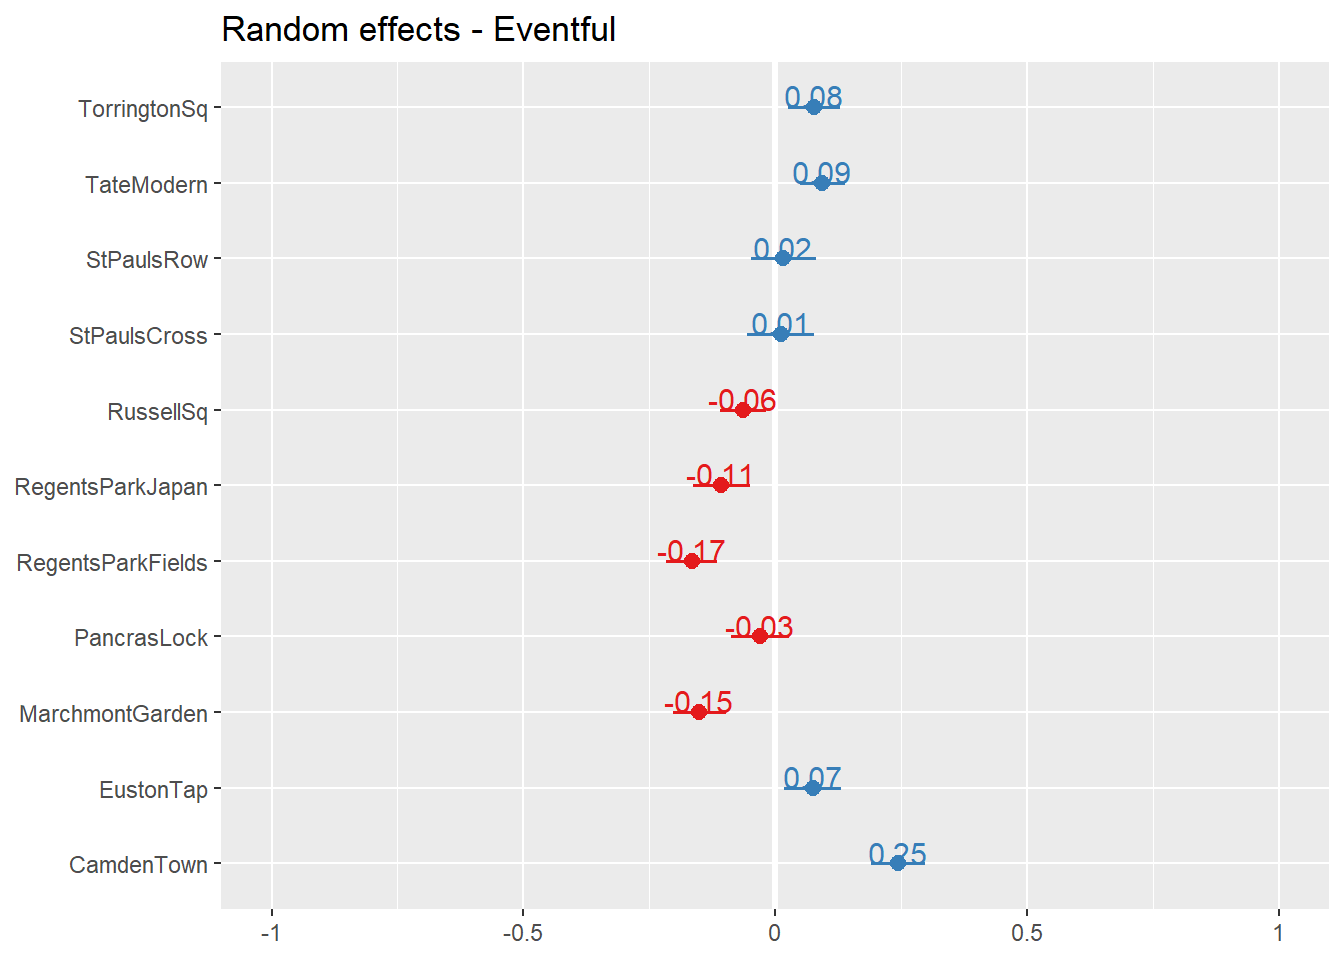
\includegraphics[width=\linewidth]{Figures/whoRandEvNew.png}
  \end{minipage}
  \caption{The summary result demonstrated in the random-effects figures gives the average from the distribution of \gls{isopl} across locations.\label{fig:whoRand}}

\end{figure}


\subsubsection*{Occupation status}
According to our findings, occupation status, in particular `retirement' and to a lesser degree, gender (male) were important factors in the pattern of soundscape assessments. It is not clear why occupation (rather not say) demonstrates such a strong predictive relationship, either on its own or as an interaction term with \gls{who5}. A more detailed study or analysis will need to be performed to determine whether any other patterns around those who prefer not to state their occupation status can be found; it is possible that those who prefer not to say have some other characteristic which links them and somehow contributes to a change in their soundscape perception. We considered that `rather not say' may be viewed as the default response for some people, so if they were confused about the question or didn't fit in some other category, they would elect not to response. However, this seems unlikely given that both `other' and `student' (possibly the most likely group to be unsure how to respond about their occupational status) were also options and did not reveal a strong relationship.

It is worthwhile to highlight that `retirement' factor could potentially be a proxy for age (>65) and gender (male). In order to further investigate the effect which the inclusion of occupational status had on the model building process, I re-ran the stepwise feature selection, this time without including occupation status in the initial model. This allowed me to determine whether other features (namely age and gender) would be finally selected and how they would interact within the model. The results of this process are given in \cref{tab:whoLMER2}.

\begin{table}
\centering
\caption{Linear mixed effects model resulting from the feature selection process when the initial model does not include occupational status. **$p<0.01$, *$p>0.05$  \label{tab:whoLMER2}}
\label{tab:whoLMER2}
\resizebox{\linewidth}{!}{%
\begin{tabular}{lccc|ccc} 
\toprule
 & \multicolumn{3}{c|}{\textbf{ISOPleasant}} & \multicolumn{3}{c}{\textbf{ISOEventful}} \\ 
\midrule
\textbf{Predictor} & \textbf{Estimates} & \textbf{Std. Est.} & \textbf{95\% CI} & \textbf{Estimates} & \textbf{Std. Est.} & \textbf{95\% CI} \\
WHO-5 & 0.001** & \textbf{0.03} & 0.01, 0.05 & - & - & - \\
Age & \textbf{0.001*} & \textbf{0.02} & 0.001, 0.04 & \textbf{-0.001**} & \textbf{-0.03} & -0.05, -0.01 \\
Gender (male) & - & - & - & \textbf{-0.04*} & \textbf{-0.04} & -0.07, -0.001 \\
Ethnicity & - & - & - & \textbf{-0.09**} & \textbf{-0.09} & 0.03, 0.14 \\ 
\midrule
\multicolumn{7}{l}{\textbf{Random Effects}} \\ 
\midrule
$\sigma^2$ & \multicolumn{3}{l|}{0.11} & \multicolumn{3}{l}{0.08} \\
$\tau_00$ & \multicolumn{3}{l|}{0.06$_{Location}$} & \multicolumn{3}{l}{0.01$_{Location}$} \\
ICC & \multicolumn{3}{l|}{0.34} & \multicolumn{3}{l}{0.14} \\
N & \multicolumn{3}{l|}{11} & \multicolumn{3}{l}{11} \\ 
\midrule
Observations & \multicolumn{3}{l|}{1134} & \multicolumn{3}{l}{1134} \\
Marginal/Conditional $R^2$ & \multicolumn{3}{l|}{0.009 / 0.345} & \multicolumn{3}{l}{0.023 / 0.165} \\
AIC & \multicolumn{3}{l|}{778.271} & \multicolumn{3}{l}{456.130} \\
\bottomrule
\end{tabular}
}
\end{table}

Age (\gls{isopl}: $\beta=0.02, p=0.05$; \gls{isoev}: $\beta=-0.03, p=0.01$) and gender (\gls{isoev}: $\beta=-0.04, p=0.05$) then came out as significant, as shown in \cref{tab:whoLMER2}. This would indicate that occupation status, particularly `retirement', represents a group of older male individuals. Even though incorporation of occupation into the model complicates the interpretation of the outcome, it results in a slightly better fitting model ($R^2_c$ for \gls{isopl} (0.354) and \gls{isoev} (0.181)) relative to 0.345 for \gls{isopl} and 0.165 for \gls{isoev} in the model without occupation status, which is why it is selected by the feature selection process. These findings are in line with previous research, suggesting significant differences among age groups in the soundscape of different acoustic environments \citep{Ren2016Soundscape,Yang2005Acoustic}. These findings imply that an increase in age leads to an increase in the positive appraisal of the soundscape pleasantness. This is supported by a study by \citet{Aydin2016Assessment} in which they found that soundscape pleasantness reported by young individuals was significantly lower than the other age groups.

Age could potentially highlight the contextual role of the acoustic environment. Past experiences, memories, and even traumas give a particular context to our perception and shape the soundscape, making individual perception highly diverse, depending on the content of experience/memory. While the increase in age can lead to appreciating different sound elements, lower age seems to be related to more arousing and vibrant sounds \citep{Yang2005Acoustic}.

Like age, gender was found to be associated with the soundscape eventfulness. Past works have also reported that there are gender-related discrepancies in soundscape \citep{Croome1977Noise,Yang2005Acoustic}. These differences may be an indication of different auditory processing across genders.

In order to further investigate the effect which the inclusion of occupational status had on the model building process, I re-ran the stepwise feature selection, this time without including occupation status in the initial model. This allowed me to determine whether other features (namely age and gender) would be finally selected and how they would interact within the model. The results of this process are given in \cref{tab:whoLMER2}.

From the results of this model it can be seen that indeed age is selected as a feature for \gls{isopl} while now ethnicity is selected for \gls{isoev}. As shown in \cref{tab:whoCorr}, occupation is significantly correlated with both of these factors indicating that indeed it may have been acting as a proxy for them in the initial feature selection process. The $R^2$
 values for both new models -- and especially the marginal $R^2$ accounting for the fixed effects themselves -- are substantially lower in this second model than in the initial model, now accounting for only 0.9\% of the explained variance in \gls{isopl} and 2.3\% in \gls{isoev}. This would indicate that, although age, gender, and ethnicity may be significant features on their own, occupation (specifically retirement) is a significant effect on its own. 

\subsubsection*{Soundscape pleasantness and eventfulness differences among locations}

The pleasantness and eventfulness were significantly different among locations. Pleasantness appeared to be highest in locations dominated by nature sounds (i.e. Regents Park Japan). In agreement with my results, \citet{Payne2013production} referred to the pleasantness dimension of the soundscape as the positive perception of natural places as well as the restorative capacity of the soundscape. \citet{Zhang2014Research} also reported a significant impact of natural soundscape on individuals' restorative experiences and boosting pleasantness. In the study by \citet{Axelsson2010principal} participants reported that the sound excerpts of natural components are more pleasant than human and technical sounds. Unlike pleasantness, the eventfulness increased the most in locations with dominant traffic and other sounds (i.e. Euston Tap). These findings are supported by previous research done by \citet{Bradley2000Emotion} and \citet{Hume2013Physiological}. In both studies, unnatural and urban sound-clips (i.e. fire engine siren and traffic noise), inherent in the traffic-dominant locations in this chapter, were rated highest in arousal and lowest in the pleasantness dimension. As formerly mentioned by \citet{Erfanian2019Psychophysiological}, throughout the soundscape literature, arousal has been applied as the equivalent of eventfulness and indicated on the Y-axis of the circumplex model \citep{Axelsson2010principal,Erfanian2019Psychophysiological}.


These results insinuate the notion that there are multiple primary factors \citep{Bradley2000Emotion} that contribute to the perception of the acoustic environment which should be considered important by urban designers and policymakers. It is expected that understanding these factors will provide multidimensional knowledge in guiding the implementation of the technological infrastructure of smart cities.

\section{Discussion}
The goal of this chapter was to determine to what extent secondary factors mediate soundscape perception, and to highlight which of these secondary factors are important to consider. 

As expected, the majority of the total variance in the perceptual ratings is explained by the location-level differences (i.e. overall sound level) which represent primary contributing factors to the acoustic environment (see \citep{McDermott2012Auditory}) and other non-acoustic factors. Approximately 3\% of the variance is then explained by the combination of personal factors, which represent secondary contributing factors as defined by McDermott. Although the variance explained by these secondary factors is small compared to the primary factors, they are still found to contribute significantly. Furthermore an additional 3 percentage points of explained variance would represent a meaningful improvement in the performance of predictive soundscape models based on in-situ measurements of varying soundscape types \citep{Lionello2020systematic} and should therefore be considered when constructing these models.

% \copied{My initial assumption was that an increased level of psychological well-being is associated with increased pleasantness and eventfulness assessments of the soundscape. Although the results showed that psychological well-being was positively associated with pleasantness, it was negatively associated with eventfulness in males and individuals that did not report their occupation.}

% \copied{Then I hypothesized that differences in soundscape assessments are associated with demographic features. The results suport this hypothesis to a certain degree. Occupation and gender appeared to be strong demographic factors influencing the pleasantness and eventfulness assessment. Retirement as occupation status showed to be positively attribute to pleasantness and negatively to the eventfulness assessment. Further investigation revealed that the occupation (no occupation reported) was negatively associated with pleasantness and gender (male) was negatively associated with eventfulness, whereas unemployment was positively associated with eventfulness.}

\subsection{Incorporating personal factors}
Although, as \citet{Droumeva2021sound} points out, each individual brings their own cultural and subjective aspects of listening to the stage of urban sound, when attempting to characterise the soundscape of a space, it is not a particular individual's aspects we should be concerned with. That individual forms a part of the collective perception of the space. Their cultural and subjective (i.e. personal) aspects mitigate their perception, but this perception then forms only a single component of the collective perception. How then should we consider these personal factors? Surely there is no suggestion to disregard their influence and importance within the soundscape approach? In my view, there are two approaches:

\begin{enumerate}
  \item Incorporate these personal factors as demographic statistics of a location; or
  \item An agent-based approach where each individual likely to use the space is simulated and modelled with their personal factors to then be included in the collective perception.
\end{enumerate}

Let's look at how these two approaches would be implemented into the multilevel acoustics-based predictive model, such as those presented in \crefrange{ch:mlmann}{ch:lockdown}.

%TODO: Expand
\subsubsection{Approach 1}
In the first, the demographic breakdown of the space under investigation is estimated, either through a census or by the designers' desired use case. This demographic breakdown can then be compared to the results presented above \citep{Erfanian2021Psychological} to derive weighting factors which adjust the predicted soundscape assessment. For instance, the results suggest that retired persons perceive the soundscape as 0.01 points more pleasant than others. If the particular space under investigation has a large proportion of retired persons, say 65\% we could then apply an adjustment to the initial personal-factors-agnostic prediction to reflect this tendency. In this example, an initial location-level \gls{isopl} prediction of 0.36, with a 65\% retired population would be corrected by 0.0065 (0.65 x 0.01) for a final demographics-corrected \gls{isopl} prediction of 0.3665.

\subsubsection{Approach 2}
In the second approach, rather than performing an overall estimation of the demographics and soundscape perception distribution, individual responses (with their own probability estimation) are modelled. To illustrate this, let's assume that the modelling is performed for a 30 second section of audio; for a given day, we would then model a single response to each 30s audio, where the individual response, including adjustments for that individual's demographic features would be modelled. For any given individual, their likely demographic profile would be randomly drawn from the estimated demographic breakdown of the space -- i.e. if the space is expected to have 40\% men and 60\% women, there would be a 40\% chance that the individual modelled for a randomly selected 30s audio is a man and the appropriate feature coefficients would be used. The multiple individual responses are then summed to give the overall distribution of responses. Again, the general demographics of the space would need to be estimated in order to ensure that a reasonable distribution is used. This is a more direct implementation of the modelling presented in this chapter, directly using the models derived in this chapter, as opposed to deriving weighting factors as in approach 1.

\subsubsection{Benefits and downsides}
Without knowing the implementation of a final model (i.e. exactly how the input data is measured and fed through the system and the structure of the model), it is difficult to know which approach would be more or less difficult to implement. Assuming a system which generates a predicted distribution of responses for each 30s recording, it seems likely that both approaches would be equally simple to implement. However, approach 2 seems to offer one useful advantage; by applying the demographic corrections to each individual response prediction, it would be easier to appropriately include estimates for intra-correlated demographic characteristics. For instance, as illustrated in \cref{tab:whoLMER}, the \gls{isoev} has an interaction factor for psychological well-being (\gls{who5}) and gender (Male), so the proper breakdown both of the gender distribution and of the psychological well-being within the genders would be required. This seems much better suited to approach 2, where any individual's full personal profile could be created based on the factors which are likely to appear together (e.g. high psychological well-being and retired may be more prevalent in men than women and this would need to be reflected in the demographic statistics). 

On the other hand, again depending on the particular implementation of the final model, approach 1 would seem to be easier to exclude personal factors. As noted in \cref{sec:modelConstraints}, a robust model should allow us to define `optional' factors - ones which can be excluded from the model. Given their low impact and difficulty to estimate, personal and demographic factors will likely not always be available to include. If they are incorporated by applying weighting factors to the model predictions, then excluding them is as simple as not adding these weighting factors. 

\section{Conclusion}
In this chapter, I conducted a linear mixed-effects model to show the associations of psychological well-being and demographic factors with soundscape pleasantness and eventfulness. The findings indicate that psychological well-being is positively associated with pleasantness and negatively associated with eventfulness in males and individuals that did not report their occupations. I further demonstrated that the occupational status, in particular retirement as a proxy of age and gender, was related to the perceptions of pleasantness and eventfulness. In total, these personal factors were shown to account for 1.4\% of the variance for pleasantness and 3.9\% of the variance for eventfulness. 

These results confirm, to some degree, the results presented in \cref{ch:mlmann}, where gender was not found to be a significant predictor of annoyance. If we take annoyance to be the inverse of pleasantness, then both analyses reveal there is not a relationship between gender and the perception of pleasantness/annoyance. However, the results of this chapter do demonstrate that gender, both on its own and when paired with psychological well-being has a significant impact on a person's perception of the eventfulness of a soundscape. This further demonstrates the limitations of previous noise control studies which, at most, aimed to investigate only the annoyance dimension. It is important to ensure that we are not disregarding the secondary dimension of soundscape perception. 

I then offer a series of proposals for how these personal factors can be included in a predictive modelling framework to enable soundscape predictions to account for differences in demographic patterns. At some point, it seems necessary that a truly holistic approach to soundscape design will need to account for these differences, particularly as we begin to make better comparisons across countries and cultures. However, given the level of uncertainty still present in soundscape predictions and the relatively low explanatory demonstrated for these demographic features, at this point it does not appear that further exploring personal factors in a predictive modelling context is the most necessary step. Other, more impactful features such as including sound sources and visual features, are more important for creating accurate and useful predictive models. That said, the inclusion of psychological well-being (as measured by \gls{who5}) does provide new empirical grounds for research to explore the influence of one's psychological state on their perception and experience of complex sound environments.

\chapter{Towards a Probabilistic Approach}
\label{ch:ProbabilisticPOC}

\subsection{Limitations of the ISO}
How these methods should be applied to represent the soundscape of a location has not been adequately discussed in previous literature, nor sufficiently in Part 3 of ISO 1293 itself. Indeed, in Section A.3, the technical specifications document state that \citep[p. 5]{ISO12913Part3}:

\begin{quote}
  Results can be reported in a two-dimensional scatter plot with coordinates for the two dimensions ‘pleasantness’ and ‘eventfulness’. The coordinates for ‘pleasantness’ are plotted on the X-axis, and the coordinates for ‘eventfulness’ on the Y-axis. Every data point in the scatter plot represents one investigated site.
\end{quote}

However, it is not made clear whether this single point on the circumplex can be considered to be a realistic representation of the average perception of the acoustic environment. Effectively, there is no representation of dispersion in the soundscape assessment, nor a recommended use of the range that was calculated as part of the analysis recommend in Section A.2 of Part 3 of the ISO 12913. Absent a suggestion from the ISO 12913 for how the range should be used, we therefore apply this analysis to an existing real-world soundscape dataset to determine whether it provides a useful measure of dispersion. Here we use the data contained in the International Soundscape Database (ISD) \citep{Mitchell2021International}, which includes 1,300+ individual responses collected across 13 locations in London and Venice, according to the SSID Protocol, which is based on the ISO methods explored in this paper \citep{Mitchell2020Soundscape}.

For any large enough sample for a site, the range will always be from 1 to 5, the maximum and minimum available Likert-scale values. We would expect that collecting more data would result in more information or better precision, however the range will always increase as the sample size increases. As an example, within the ISD data, of the 8 PAs collected at 13 locations (for a total of 104 scales), 88\% have a range from 1 to 5 and with larger sample sizes at each location, this percentage would only have increased. Using range to analyse the dispersion provides very limited information for comparing the soundscape assessments of different locations, or of a location under different conditions.

Although the range does not appear to be a useful measure of dispersion, the median does provide a useful measure and appropriately functions to describe the central tendency of the  soundscape assessment of the sample. However, by stipulating that the median of each PA should be taken prior to applying the circumplex projection, the ISO procedure only allows for plotting a single scatter point in the circumplex for each location, and does not allow for plotting individual responses on the circumplex. This limits the possibilities for visualising the general trends in individual perception across the soundscape. Finally, no example or recommendation for how the circumplex scatter plot should be presented is given in the standard.

The instruments described in the ISO 12913 Part 2 \citep{ISO12913Part2} were originally designed primarily for the context of individual or small group assessments. In these scenarios, the focus is on assessing the particular soundscape perception of the person in question. Recent advances in the soundscape approach since the development of the standards have shifted some focus from individual soundscapes to characterising the overall soundscape of public spaces \citep{Mitchell2020Soundscape} and to making comparisons between different groups of people \citep{Jeon2018cross}. In this context, a consideration of the natural variation in people's perception and the variation over time of a soundscape must be a core feature of how the soundscape is discussed. Reducing a public space which may have between tens and tens of thousands of people moving through it in a single day down to the mean (or median, or any other single metric) soundscape assessment often dismisses the reality of the space. Likewise, this overall soundscape of a public space cannot be determined through a ten person soundwalk, as there is no guarantee that the sample of people engaged in the soundwalk are representative of the users of the space (in fact it is very likely they would not be).


\section{The Way Forward: Probabilistic Soundscape Representation}
Given the identified issues with the recommended methods for statistical analysis and their shortcomings in representing the variety in perception of the soundscape in a space, how then should we discuss or present the results of these soundscape assessments? Ideally the method will: 1) take advantage of the circumplex coordinates and their ability to be displayed on a scatter plot and treated as continuous variables, 2) scale from a dataset of twenty responses to thousands of responses, 3) facilitate the comparison of the soundscapes of different locations, conditions, and groups, and 4) encapsulate the nuances and diversity of soundscape perception by representing the distribution of responses.

We therefore present a visualisation in \cref{fig:circ} of the soundscape assessments of several urban spaces included in the ISD \citep{Mitchell2021International} which reflects these goals. The specific locations selected from the ISD are chosen for demonstration only and these methods can be applied to any location. Rather than attempting to represent a single individual's soundscape or of describing a location's soundscape as a single average assessment (as in \citep{Mitchell2021Investigating}), this representation shows the whole range of perception of the users of the space. First, rather than calculating the median response to each PA in the location, then calculating the circumplex coordinates, the coordinates for each individual response are calculated. This results in a vector of ISOPleasant, ISOEventful values which are continuous variables from -1 to +1 and can be analysed statistically by calculating summary statistics (mean, standard deviation, quintiles, etc.) and through the use of regression modelling, which can often be simpler and more familiar than the recommended methods of analysing ordinal data. This also enables each individual's response to be placed within the pleasant-eventful space. All of the responses for a location can then be plotted, giving an overall scatter plot for a location, as demonstrated in (i).

\begin{figure}[!ht]
  \centering
  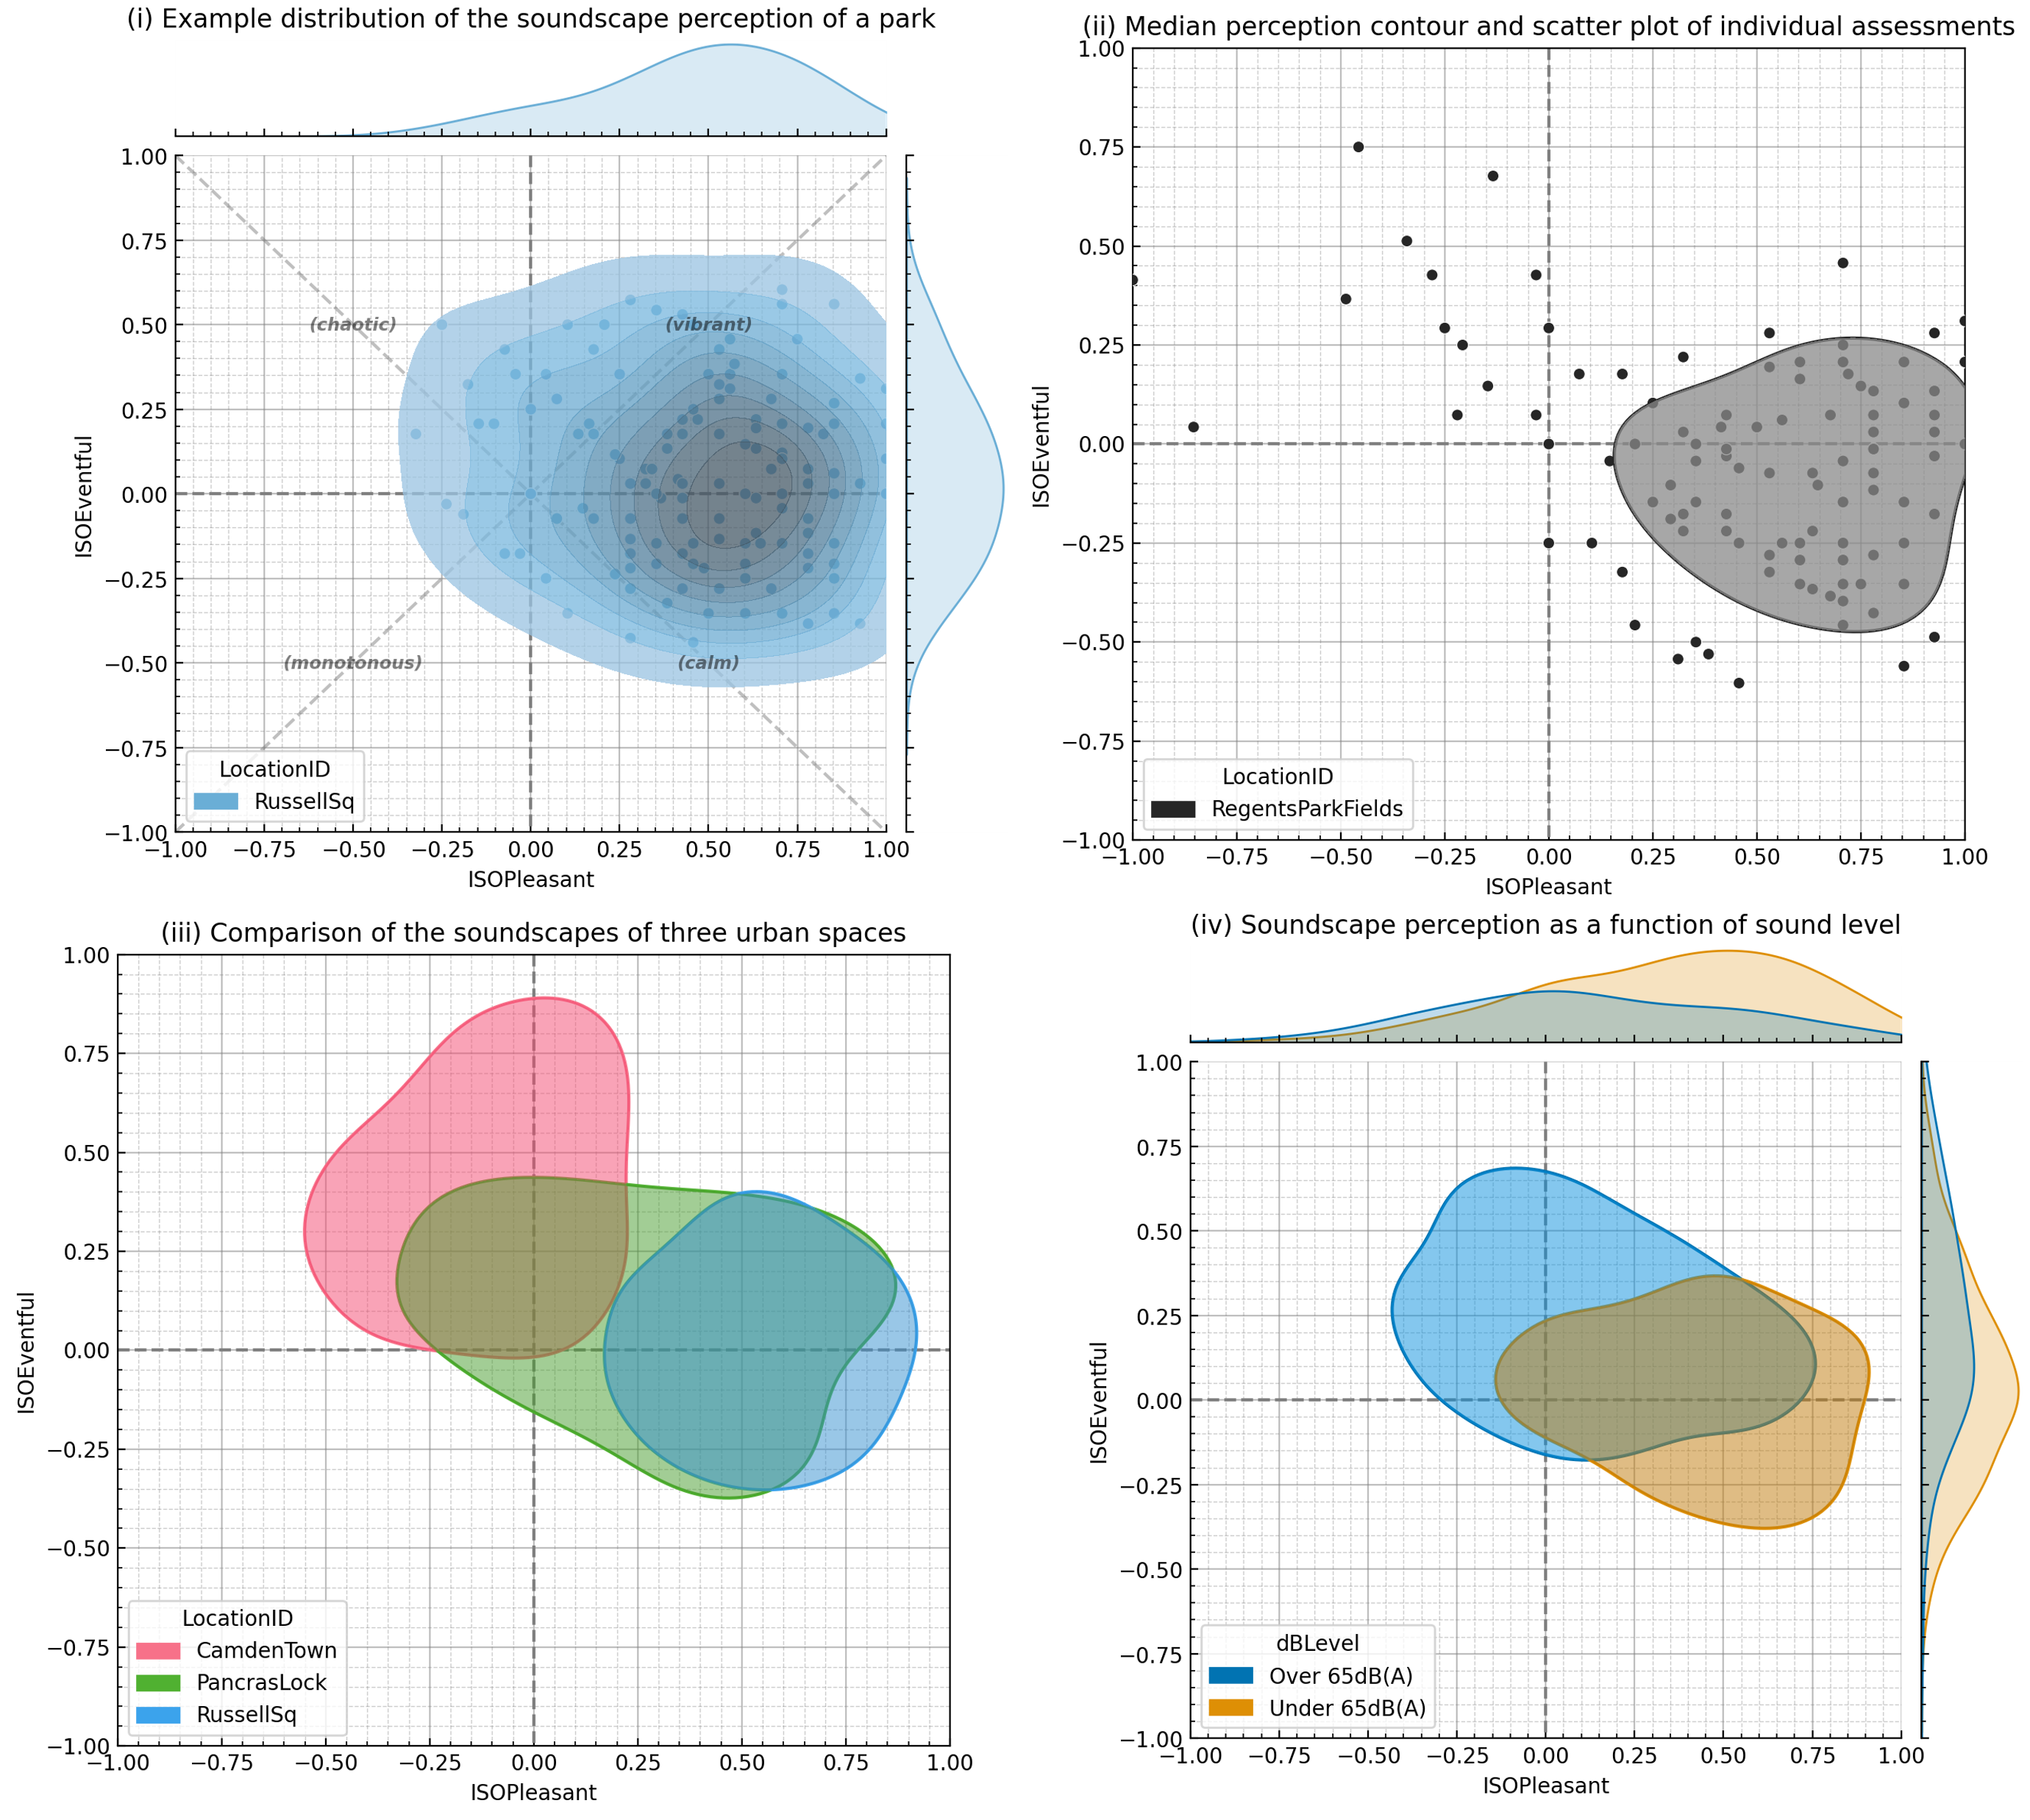
\includegraphics[width=\textwidth]{Figures/jasa-el_Figure2.png}
  \caption{\linespread{1}\selectfont{} A demonstration of some use cases of representing soundscape perception as probabilistic distributions. Data is drawn from the International Soundscape Database (ISD) and is used for demonstration only. (i) Demonstrates a high-level of detail for presenting the bivariate distribution of soundscape perception in a park (Russell Square in London). (ii) Simplified view of the distribution using the \nth{50} percentile contour. The assessments impacted by a series of helicopter fly-overs are made obvious in the chaotic quadrant. (iii) A comparison of three popular public spaces in London. Their overlapping regions can reveal when and how their soundscapes may be similar. (iv) A comparison across the full ISD for soundscape perception at $<65 dB L_{Aeq}$ and $> 65 dBA$. The introduction of other acoustic, environmental, and contextual data can reveal new and complex relationships with the soundscape perception. \label{fig:circ}}
\end{figure}

Once these individual responses are plotted, we then overlay a heatmap of the bivariate distribution (with isodensity curves for each decile) and marginal distribution plots. In this way, three primary characteristics of the soundscape perception can be seen:

\begin{enumerate}
  \item The distribution across both pleasantness and eventfulness, including the central tendency, the dispersion, and any skewness in the response;
  \item The general shape of the soundscape within the space - in this case Russell Sq is almost entirely in the pleasant half, but is split relatively evenly across the eventfulness space, meaning while it is perceived as generally pleasant, it is not strongly calm or vibrant;
  \item The degree of agreement about the soundscape perception among the sample - there appears to be a relatively high agreement about the character of Russell Sq, as demonstrated by the compactness of the distribution, but this is not the case for every location.
\end{enumerate}

Fig (i) includes several in-depth visualisations of the distribution of soundscape assessments, however the detail included can make further analysis difficult. In particular, a decile heatmap is so visually busy that, in our experience, it is not possible to plot more than one soundscape distribution at a time without the figure becoming overly busy. It also can make it difficult to truly grasp point 2, the general shape of the soundscape. To facilitate this, the soundscape can be represented by its \nth{50} percentile contour, as demonstrated in Fig (ii) where the shaded portion contains 50\% of the responses. This simplified view of the distribution presents several advantages, as is demonstrated in Figs. (iii and iv) and takes inspiration from the recommendation in the ISO standard to use the median as a summary statistic. In our testing, the \nth{50} percentile contour has proved useful, clear, and compact, however this should not be taken as the definitive correct percentile cutoff. Further work will need to be done to validate the precise presentation.

When visualised this way, it is possible to identify outliers and responses which are the result of anomalous sound events. For instance if, during a survey session at a calm park, a fleet of helicopters flies overhead, driving the participants to respond that the soundscape is highly chaotic, we would see a group of scatter points in the chaotic quadrant which appear obviously outside the general pattern of responses. Often, these responses would be entirely discarded as outliers or the surveys and soundwalks would be halted entirely -- ignoring what is in fact a significant impact on that location, its soundscape, and how useful it may be for the community. Alternatively, they would be naively included within the statistical analysis, significantly impacting the central tendency and dispersion metrics (i.e. median and range) without consideration for the context. This is the situation shown in Fig (ii) where it is obvious that there is strong agreement that Regents Park Fields is highly pleasant and calm, however we can see numerous responses which assessed it as highly chaotic. These responses were taken when a series of military helicopter fly overs drastically changed the sound environment of the space for nearly 20 minutes.

Fig (iii) demonstrates how this simplified \nth{50} percentile contour representation makes it possible to compare the soundscape of several locations in a sophisticated way. The soundscape assessments of three urban spaces, Camden Town, Pancras Lock, and Russell Square, are shown overlaid with each other. We can see that Camden Town, a busy and crowded street corner with high levels of traffic noise and amplified music, is generally perceived as chaotic, but the median contour shape which characterises it also crosses over into the vibrant quadrant. We can also see that, for a part of the sample, Russell Square and Pancras Lock are both perceived as similarly pleasant, however some portion of the responses perceived Pancras Lock as being somewhat chaotic and annoying. This kind of visualisation is able to highlight these similarities between the soundscapes in the locations and identify how they differ. From here, further investigation could lead us to answer what factors led to those people perceiving the location as unpleasant, and what similarities the soundscape of Pancras Lock has with Russell Square that could perhaps be enhanced to increase the proportion of people perceiving it as more pleasant.

In addition to solely analysing the distributions of the perceptual responses themselves, this method can also be combined with other acoustic, environmental, and contextual data. The final example, in Fig (iv) demonstrates how this method can better demonstrate the complex relationships between acoustic features of the sound environment and the soundscape perception. The data in the ISD includes ~30-s-long binaural audio recordings taken while each participant was responding to the soundscape survey, providing an indication of the exact sound environment they were exposed to. For Fig (iv) the entire dataset of 1,338 responses at all 13 locations has been split according to the analysis of these recordings giving a set of less than 65 dB $L_{Aeq}$ and a set of more than 65 dB. The bivariate distribution of these two conditions are then plotted.

By presenting soundscape perception as a bivariate distributional shape on the circumplex, practitioners are obligated to address two key aspects of perception that are too often ignored: the distribution of potential responses and the eventful dimension. The array of potential responses to an environment is a crucial factor in assessing the successful design of a space and represents the reality of perception. There is no single perceptual outcome of an environment; it will always include some randomness inherent in human perception and this should be reflected in how we present soundscape assessments. Similarly, the eventful dimension is crucial to understanding how an environment is perceived and can have important impacts on the health and well-being of the users. Recent evidence also suggests that there is a more direct relationship between acoustic characteristics and the perception of eventfulness, while pleasantness is more dependent on context \citep{Mitchell2021Investigating}. Studies which explore the correlations between acoustic features and annoyance (or pleasantness) without considering eventfulness are perhaps missing the most direct effect of the acoustic features.

A library of plotting functions for producing the type of plots presented here has been made available as part of the ISD at \href{https://zenodo.org/record/5705908}{https://zenodo.org/record/5705908}. In addition, an interactive code notebook for this paper is included which provides a tutorial for using this code, working with the ISD data, and recreating the figures of this paper. The figures were created using the seaborn \citep{Waskom2021seaborn} and Matplotlib \citep{Hunter2007Matplotlib} plotting libraries in Python v3.92 \citep{VanRossum2009}.

\section{Making Use of the Soundscape Circumplex}
There are various potential methods for integrating the probabilistic soundscape approach into a design and intervention setting. Representing the soundscape as a shape within the circumplex provides flexibility in setting design goals for a space. Not all spaces can or should have the same soundscape and soundscapes should be treated as dynamic, not static; identifying and creating an appropriate soundscape for the particular use case of a space is crucial to guiding its design. Proper forward-looking design of a soundscape would involve defining the desired shape and distribution of perceptions in the space. This can be achieved by drawing the desired shape in the circumplex and testing interventions which will bring the existing soundscape closer to the desired perception. A soundscape may need to be perceived as vibrant during the day and calm for some portion of the evening, meaning the desired shape should primarily sit within the vibrant quadrant but have some overlap into calm. This also enables designers to recognise the limitations of their environment and acknowledge that it is not always possible to transform a highly chaotic soundscape into a calm one. In these cases, instead the focus should be placed on shifting the distribution to some degree in a positive direction. The most sophisticated method of setting design goals is therefore to identify the desired shape which represents the variety of desired outcomes, and focus on designs and interventions which are most successful in matching the predicted outcome with that goal.

Although the visualisations shown in \cref{fig:circ} are a powerful tool for viewing, analysing, and discussing the multi-dimensional aspects of soundscape perception, there are certainly cases where simpler metrics are needed to aid discussion and to set design goals. Taking inspiration from noise annoyance \citep{ISO15666}, we propose a move toward discussing the "percent of people likely to perceive" a soundscape as pleasant, vibrant, etc. when it is necessary to use numerical descriptions. In this way, a numerical design goal could also be set as e.g. `the soundscape should be likely to be perceived as pleasant by at least 75\% of users' or the result of an intervention presented as e.g. `the likelihood of the soundscape being perceived as calm increased from 30\% to 55\%'. These numbers can be drawn from either actual surveys or from the results of predictive models.

Finally, although acknowledging the distribution of responses is crucial, it is sometimes necessary to summarise locations down to a single point to compare many different locations and to easily investigate how the soundscape assessment has generally changed over time. For this purpose, the mean of the ISOPleasant and ISOEventful values across all respondents is calculated to result in a single coordinate point per location. This clearly mirrors the original intent of the coordinate transformation presented in the ISO, but by applying the transformation first to each individual assessment then calculating the mean value, it maintains a direct link to the distributions shown in \cref{fig:circ}. An example plot using the mean response of each location to compare many locations and to demonstrate change in soundscape perception can be found in Figure 5 of \citet{Mitchell2021Investigating}. The key to all of these analysis methods, whether they be the distributional plots shown in \cref{fig:circ}, the numerical summaries, or the use of other standard statistical analyses is treating the soundscape of the space or group as a collective perception as expressed by a vector of individual circumplex coordinates.

\subsection{Incorporating appropriateness}

The discussion thus far has focussed on the two primary dimensions of soundscape perception - pleasantness and eventfulness. Our next goal is to somehow account for the third primary component identified by \citet{Axelsson2010principal} - Familiarity, sometimes also referred to as Appropriateness. In a later paper, \citet{Axelsson2015How} addresses critiques of the \gls{ssqp} for its focus on perceptual attributes and its use of a Good-Bad scale, without considering the appropriateness of the soundscape. %TODO Return here


\subsection{Limitations of the circumplex and quantitative analysis}
The method presented here is a solution for representing the soundscape of a space, which requires considering the perception of many people, but it is important to note that this is only one (very important) goal of the soundscape approach. Psychological and sociological investigations of people's relationship to their sound environment and the interactions between social contexts and individual perception are a crucial aspect of the field for which this approach would likely not be sufficient \citep{Bild2018Public}. Open-response questions, structured interviews, and mixed-methods studies can provide additional insight into how people experience their environment and should be considered alongside or preceding this focus on how a space is likely to be perceived on a larger scale.

These other approaches are not in opposition to the methods proposed here, but instead further expand our view. The circumplex is a limited view of soundscape perception (this is made obvious by the fact that it excludes the third component, \emph{familiarity}, identified in \citet{Axelsson2010principal}) but it is an exceptionally rich tool for dealing with the two primary aspects of soundscape perception which can readily expand the much more limited view provided by existing noise and annoyance assessment tools. Aspects of the psychological and sociological emphasis can also be integrated into a circumplex-focused approach, as demonstrated in \citet{Erfanian2021Psychological}, where personal factors such as age, gender, and psychological well-being were analysed in terms of how they mediated the ISOPleasant and ISOEventful outcomes.

It should also be noted that the particular PA descriptors used in ISO 12913 are intended for outdoor environments and should not be directly applied to indoor spaces. However, a proposed set of descriptors for some indoor environments has been derived which further confirms the validity of the circumplex relationships \citep{Torresin2020Indoor}. The methods proposed here should be directly applicable to indoor spaces by using the comfort/content descriptors as well as to any other translations of soundscape descriptors into other languages \citep{Aletta2020Soundscape} as long as the dimensional relationships of the circumplex are maintained.


\section{Conclusions}
Soundscape studies have been steadily growing as a research field over the past three decades. Their relevance for the planning and design of urban spaces is now generally acknowledged by both the academic and practitioners' communities. Yet, for their contribution in shaping better environments to be meaningful, it is necessary to agree on common methodological approaches and techniques to analyse and present standardised soundscape data. Therefore, the general goal of this work is to consider some of the questions that may still have been left unanswered by the ISO 12913 series when it comes to optimal ways to analyse and represent soundscape data coming from the ISO standardised protocols. As a result, we propose a method for presenting the results of standardised
assessments as a distribution of soundscape perception within the circumplex space. This method provides an opportunity to conduct a nuanced discussion of soundscape perception which considers the variety of individual responses. The tools for generating these circumplex visualisation is made openly available as well. This shift is part of a move towards a more holistic approach to urban noise and to integrating the soundscape approach into urban design and regulations.

%%%%%%%%%%%%%%%%%%%%%%%%%%%%%%%%%%%%%%%%%%%%%%%%%%%%%%%%%%%%%%%%%%%%%%%%%

\draft{======= Random bits to incorporate somewhere =======}
\subsubsection{Sound perception as a chaotic system}

Human perception of sound is a chaotic system. Given small changes in a large number of input conditions, a wide range of outcomes are possible \cit{some chaos theory thing}. The same person, exposed to the same environment, could have very different responses to it depending on their state of mind, the route they took to get to the space, what they ate for breakfast, or even just some inherent randomness in their psychological response. This is further amplified by the innumerable differences between people which it will never be possible to fully capture. This is all the more true when discussing in situ perception, outside the controlled conditions of a laboratory.

However, the wide array of previous literature demonstrates that, when taken as a statistical group, conclusions can be made about the probable soundscape perception and its various causal factors.

\begin{quote}
  It means that in many situations, all we can say about a system's dynamics is of a statistical nature. -Gert van der Hejden
\end{quote}

\section{Interpreting the Soundscape Circumplex}
%Move this paragraph to the interpretation of the circumplex section.
The circumplex model of soundscape, as originally defined by \citet{Axelsson2010principal}, is commonly understood to be a two-dimensional space (its main orthogonal components being annoying-pleasant and uneventful-eventful) where all regions of the space are equally likely to accommodate a given soundscape assessment \citep{Aletta2016Soundscape}. For instance, in theory, an extremely vibrant soundscape (e.g., with a score of 1) should be as likely to occur as an extremely annoying one, as well as one neutral on all dimensions (e.g., with a score of 0). However, a recent work by Lionello et al. \citep{Lionello2021Introducing} incidentally highlighted a possible issue with the process for representing soundscape assessments with the current ISO protocols. More specifically, when considering big numbers, soundscape assessments seem to have a bivariate normal distribution around the origin of the circumplex model. This would imply that not the whole space of the model is equally accessible to any given soundscape. Studies in the field show that data collection campaigns rarely return extreme values for soundscape dimensions \citep{Mancini2021Soundwalk} and so far the general interpretation has been that some soundscapes (e.g., extremely monotonous) may simply be difficult to find and detect with people in urban contexts \citep{Sun2019Classification}.

\subsection{Application \& Simulations}
In order to investigate the shape of the circumplex coordinate space generated by this transformation, a dataset of 3 million randomly simulated PA responses was generated. For each of the 8 PAs, an integer value from 1 to 5 is randomly generated from a uniform distribution, meaning each of the five responses is equally likely. These simulated data are specifically not intended to include any information about correlations between the various PAs when actually answered by respondents (see \citep{Lionello2021Introducing} for more on this discussion), instead the PA responses are completely uncorrelated as they each have their own random distribution. Therefore, the simulated dataset represents a theoretical uniform coverage of the 8 dimensional PA space.

We then apply the ISO transformations given in \cref{eqn:pleasant,eqn:eventful}, resulting in 3 million coordinate pairs with a range of (-1, 1) in the x and y axes. A heatmap of the resulting two-dimensional circumplex space is shown in \cref{fig:isoheatmap}, along with histograms of the individual dimension distributions. These distributions then represent the theoretical available circumplex space generated by the ISO transformation on uniform survey responses.

\begin{figure}
  %TODO: Insert heatmap figure, with histograms/distribution plots of individual axes
  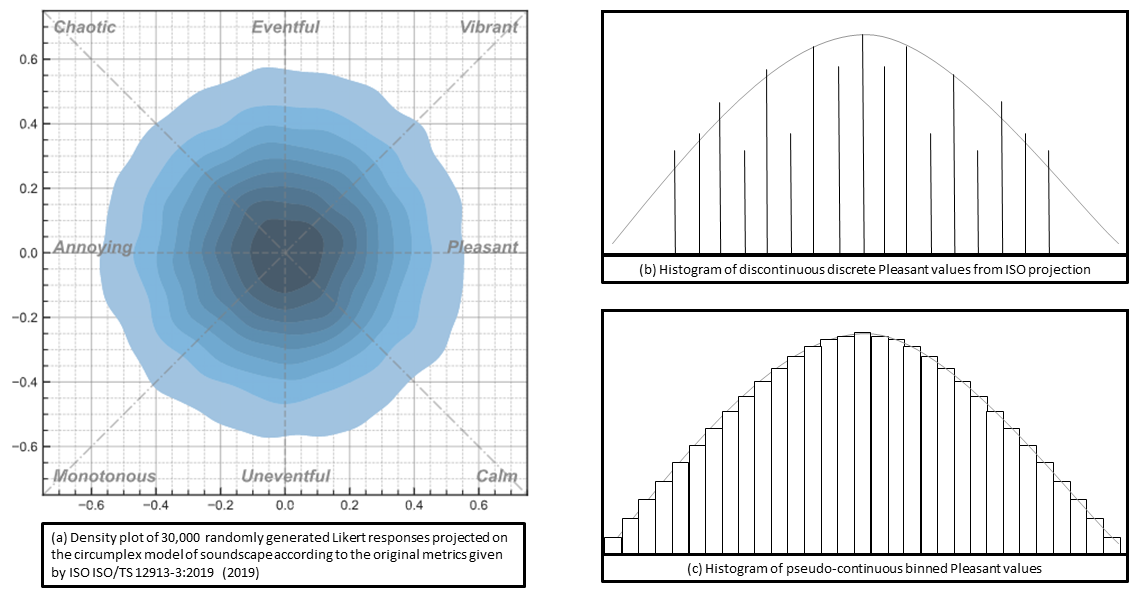
\includegraphics[width=\textwidth]{figures/Combined_sim_hist_mockup.png}
  \caption{Mockup placeholder simulation heatmap plot from Lionello 2020 and discrete vs binned transformation values. For new one, need to include distribution histograms along each axis.%
    \label{fig:isoheatmap}
  }
\end{figure}

Two important observations can be made about the shape of the resulting two-dimensional distribution. The first is that the shape of the available space is a circle. It should be noted that, despite what the term 'circumplex' may indicate, the perceptual dimensions are not necessarily intended to circumscribe a circle. The second is that, in each dimension, the responses are normally distributed, centered around zero. These points will be discussed in detail below.

\subsection{Circular space discussion}
%TODO: fill in circular discussion.
Visualisations of the circumplex model in soundscape literature tend to present it as circumscribing a circle (see Figure 1 in \citep{Axelsson2010principal} and Figure 3 in \citep{Torresin2020Indoor}), and this shape is further emphasised by the initial figure in \citet{Russell1980circumplex}'s original formulation of the concept. However, it should be emphatically noted that all of these presentations are in fact artefacts of the analysis methods which generated them, not some sort of revealed pattern in the component attributes which make up the circumplex. In \citet{Russell1980circumplex}, this first figure is generated by asking respondents to place each of the 27 attributes around a circle, according to their perceived spatial relationships - the circle shape was pre-imposed on the study. In both \citet{Axelsson2010principal} and \citet{Torresin2020Indoor}, the figures are generated via Principle Components Analysis (PCA) which, again, presents these results superimposed on a circle. It is perhaps a weakness of these two, otherwise strong and impactful, papers, that they did not recognise this consequence and challenge the circular arrangement.

If we turn back to Russell's original work on the circumplex model of affect, we can see some indications that a circle does not, in fact, describe the spatial relationship of the perceptual attributes. Fig. 4 of \citep{Russell1980circumplex}, which did not pre-impose the circular arrangement in its analysis, instead most closely resembles a square with rounded corners. Continuing from this conception, when Russell presents a graphical method of assessing the two dimensions of affect (pleasure and arousal) \citep{Russell1989Affect}, they use a square grid. This is all to say that, although the term 'circumplex' and the foundational analyses which lead to a soundscape circumplex may lead us to assume it must take the form of a circle, both the framework laid down by Russell and the common treatment of the spatial relationships of the attributes actually describe a square, instead.

This treatment of the 8 PAs makes several assumptions and inferences about the relationships between the dimensions. As stated in the standard \citep[p. 5]{ISO12913Part3}:

\begin{quote}
  According to the two-dimensional model, vibrant soundscapes are both pleasant and eventful, chaotic soundscapes are both eventful and unpleasant, monotonous soundscapes are both unpleasant and uneventful, and finally calm soundscapes are both uneventful and pleasant.
\end{quote}

From this, we would infer that a maximally vibrant soundscape is both maximally pleasant and maximally eventful. However, when the projection transformation is applied it imposes certain limitations on the relationships between the dimensions which do not conform with this assumption. As shown in \cref{fig:radar}, when a soundscape is maximally vibrant (i.e. a diagonal vector distance of 1), the maximum pleasantness value it can have is determined by the $\cos 45\degree$ term, giving a max pleasantness value of $\sim0.7071$. The implication of this is that no soundscape can be both maximally pleasant and maximally eventful at the same time, meaning that these dimensions are not in fact considered as orthogonal, and that a highly vibrant soundscape cannot be considered highly pleasant or highly eventful. Similarly, if a soundscape were to begin at a maximum Eventfulness, with neutral Pleasantness, in order for the soundscape to become more pleasant, it must by definition become less eventful. This is not conceptually correct or borne out in the treatments of previous literature. These same relationships and violations hold true for the other diagonal dimensions, chaotic, calm, and monotonous.

This implication violates both the assumptions made within the formulation of the circumplex model and the way that soundscape practitioners have understood and presented the interpretations of soundscapes within the circumplex space. In cases where the PA dimensions are referred to directly \citep{steele2016evaluation, steele2019soundtracking} and those which have made use of the Part 3 transformation to 2-dimensional coordinates \citep{Mancini2021Soundwalk, Lionello2021Introducing, Manzano2021importance}, \emph{Check Manzano2021importance} the conflation of maximal values on the diagonal axes with maximal values on the primary axes is made, as in the assumptions made by the standard. This is the first of the common understandings of the circumplex which are violated by the trigonometric transformation.

\subsection{Normal distribution discussion}
%TODO: fill in normal discussion

We can also see from the histograms included along the axes of \cref{fig:isoheatmap} that the projection creates a normal distribution in both dimensions. % TODO: edit this phrasing to match the final figure
It is important here to remember that the input to the projection formulas were uniform distributions for each of the 8 PAs, and it is the projection into the two primary dimensions which results in this normal distribution.
From the simulated distributions, we can derive a normal probability density distribution (PDF) for each of the dimensions.

\[   f_X(x) = \frac{x^{-(x-\mu)^2/(2\sigma^2)}}{\sigma \sqrt{2\pi}}\]
% ! TODO: Need to pull the actual standard deviation value.
with a mean $\mu = 0$ and standard deviation $\sigma = 0.3$.

\paragraph*{Realistic max values}
% ! TODO: Andrew update this with the actual values from the calculations!
When looking at the distribution heatmap in \cref{fig:isoheatmap}, it is useful to picture the gradients as representing the available space in the circumplex model. The probability of reaching a given result decreases as we move farther away from the origin. This means, for example, that the probability of getting a pleasantness value between 0.2 and 0.3 is nearly 4 times the probability of getting a value between 0.5 and 0.6. This may not seem important, but the consequence is that, as a result of strictly the projection calculation, neutral values within the soundscape circumplex are much more likely and the space available to compare soundscapes within is truncated.

When we start to think about real-world urban soundscape data collection, where the discussion of the soundscape of a space is not limited to a single person's perception, we need to start thinking in statistical terms. Theoretically, the limits of the projected Pleasantness are (-1, +1), however according to the PDF calculated above less than 10\% of values fall outside the range (-0.5, +0.5).
% Note: Maybe this should be moved to Proposals or Discussion section?
It may be argued that as long as +1 can theoretically be reached, this should be what is considered the maximum value for that dimension. However, in any situation which involves using multiple individual soundscape assessments in order to characterize the overall soundscape of a location, this max will effectively never be reached. According to the large-scale, multi-location data set reported in our previous study, it appears that the effective maximum values for Pleasantness and Eventfulness for the combined assessment of multiple people for a space is in reality approximately (-0.6, +0.6) \citep{Lionello2021Introducing}.

As such, extreme values on each of the perceptual dimensions are less likely to occur than are coordinate values which place the soundscape in the neutral areas of the circumplex space. This means an extremely calm (or chaotic, or vibrant, or pleasant) coordinate is significantly less likely to occur than a neutral coordinate.


\subsection{Non-continuous projected values}
% Very brief presentation of this potential issue
An implicit assumption of the transformation is that the resulting coordinates are now continuous values, which allows linear regression and correlation methods to be used. Indeed, the transformation of the 8-dimensional ordinal Likert scale data to the two-dimensional coordinates creates a higher resolution of intervals, which would appear to be pseudo-continuous. Upon further investigation, the transformation actually results in XX discrete possible values. \cref{fig:isoheatmap}(b) shows a histogram of this raw output from the transformation, demonstrating that these discrete values, while following the general normal distribution discussed above, are not evenly filled - some adjacent values may be much more or less likely than their neighbours. This poses potential issues for further analysis which assumes either continuous or equally-spaced discrete values.


\section{Probabilistic predictions - A Bayesian Approach?}

\subsection{Defining a distribution}

\subsubsection{Truncated normal distribution}

Given that the \gls{isopl} and \gls{isoev} values have a hard boundary at $[-1, +1]$, it is not in fact correct to consider the distribution of responses within the circumplex as a normal distribution. A normal distribution is defined as extending out to $(-\infty, \infty)$ with an area of 1 under the probability density. If the potential space of the responses is bounded, the assumption of them forming a normal distribution is violated, as part of the probability density function is unreachable, meaning the area under the probability density will not sum to 1.

If we assume the general shape of the responses to be normal, then they would instead form a truncated normal distribution \cit{\url{https://people.sc.fsu.edu/~jburkardt/presentations/truncated_normal.pdf}, \url{https://www.tandfonline.com/doi/abs/10.1080/00031305.1999.10474490}}. Briefly, a truncated normal distribution is estimated by first calculating the probability density function of the standard normal distribution. Then, the density function is truncated at the set boundary ($[a, \infty)$ or $(-\infty, b]$) or boundaries ($[a, b]$) and the portion of the density function which is truncated is redistributed within the boundary.

This redistribution means that the various parameters of a truncated distribution will be somewhat different than for a normal distribution, in particular the calculation of variance. This impacts the soundscape distribution plots demonstrated in \cref{ch:circumplex} as the kernel density estimation performed by the underlying plotting library (\texttt{seaborn}) assumes a normal distribution with no boundary. It is possible that making use of a truncated normal distribution would change the shape of the distributions produced by \texttt{soundscapy}. Although at this point there does not seem to be a simple method of adapting the \texttt{soundscapy} code to make use of a truncated distribution, I chose to briefly test out how much of a change the truncated distribution is likely to make to the shape of the \texttt{soundscapy} plots through functions available in \texttt{R}.

\begin{figure}
  \centering
  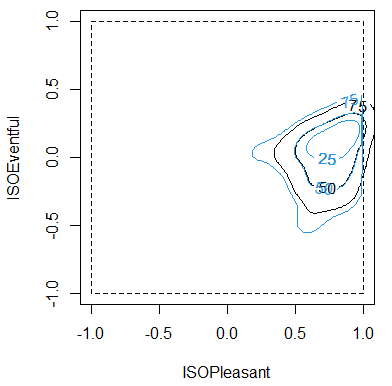
\includegraphics{Figures/Trunc-Normal-demo.png}
  \caption{Comparing a probability distribution in the soundscape circumplex (using Regents Park Japan as the worst case example) using a normal kernel density estimation method (black line) and a truncated KDE (blue line). \label{fig:truncatekde}}
\end{figure}

From \cref{fig:truncatekde}, it appears that there would be some difference in the shape of the soundscape distribution when using a truncated distribution. However, I would note that Regents Park Japan was chosen as the worst case location in the whole \gls{isd} as the samples lie closest to the boundary and the density function estimated in \texttt{soundscapy} has the most area which lies outside the boundary. Most locations do not show any overlap with the boundary and would not be noticeably affected by the truncation. In addition, switching to the truncated normal distribution only affects those iso-density levels which overlap with the boundary. Therefore, the recommended simplified density curve given in \cref{ch:circumplex} of 50\% is effectively unchanged since it is very unlikely the \nth{50} percentile curve would exceed the boundaries. For the time-being, therefore it appears that there is not a detriment to using a standard normal distribution as opposed to a truncated normal distribution, for the visualisations created by \texttt{soundscapy}.

However, as I move towards a probabilistic prediction framework, and even in the frequentist predictive models used throughout this thesis, it seems possible that the distinctions between these underlying distributions will become more important.

\section{A proof of concept for predicting the distribution of soundscape perception}

\section{Discussion}

\section{Conclusion}



\chapter{Conclusions}
\label{ch:conc}

\section{General Discussion}
\begin{itemize}
  \item Soundscape studies have been focussed for too long on the retrospective post-hoc evaluation of a space.
  
\end{itemize}

Retrospective assessment methods also struggle to capture the dynamics of the soundscape in a space. Whether through the narrative interview method of \draft{section of ISO12913-2}, through soundwalks, or through in-situ questionnaires \citep{Mitchell2020Soundscape}, only the soundscape during the particular period which the researchers are actively investigating is captured. This makes it very difficult to determine diurnal, seasonal, or yearly patterns of the soundscape. These patterns may be driven by corresponding diurnal, seasonal, or yearly patterns in the acoustic or visual environment, or by variations in how people process and respond to the sound at different times of day/season/year. Currently the only way to investigate any of these patterns is through repeated surveys. Predictive modelling, on the other hand, could allow a trained soundscape model to be paired with longterm monitoring methods to track how a soundscape may change in response to changes in the acoustic environment.

Admittedly, this method would not be able to answer the second part of the question - how do people's responses to a given acoustic and visual environment change throughout the various daily/seasonal/yearly periods? \draft{This part should maybe be moved to a discussion}One approach to answering this question which has not, as far as the author is aware, been employed is through an un-attended survey method. Such a method could involve creating and posting fliers asking users of a space to complete a soundscape survey (accessed through a QR code) and leaving these fliers installed for longer periods of time. It is unclear how successful such a general approach would be, in particular what response rate would be expected, but given the increasing familiarity with QR codes among the general public following their use for track-and-trace during COVID-19, it does appear promising. These un-attended surveys could also be paired with long-term acoustic and environmental monitoring via a WASN or powered SLM which could simultaneously track the acoustic environment. This would thus result in a time series of online soundscape questionnaires with a corresponding time series of acoustic and environmental information, allowing us to track the changes of each over long periods of time.

\begin{itemize}
  \item Soundscape has also been focussed on the local / individual scale, whereas assessment and legislation need data at the city-scale.
  \item Society ( and engineers) are interested in possibilities, in designing and improving future spaces
  \item Because of this limited view, the methods available in soundscape studies are unsuitable for these challenges.
  \item If noise control wantss to progress beyond
  \item Psychoacoustics alone is not enough to model soundscape perception
  \item To be useful, Predictive models can't include perceptual inputs, this would be recursive and self-defeating.
\end{itemize}

Predictive soundscape modelling thus provides a possibility for a more holistic approach to large scale urban sound investigations. Studies from outside of soundscape have demonstrated that a user's perception of a space is a much better predictor of how the use it -- and of the benefits they derive from it -- than the strict physical characteristics of the space \citep{Kruize2019Exploring}. It thus stands that a soundscape approach focussed on perception which can be generalised across a city-scale -- rather than in isolated spaces -- could provide more reliable metrics with which to investigate the health, social, and psychological effects of sound.

The empirical and modelling work in this thesis represents a key step towards realising this application to soundscape mapping. When the predictive modelling approach is paired with data from, e.g. a large-scale acoustic sensor network, it could be used to produce a dynamic map of the likely perception of spaces across a city. Alternatively, 
%\cit{https://reader.elsevier.com/reader/sd/pii/S0003682X17311283?token=75D2B5B9AB562DC1501F4FD072E35205CA61B84786D2ABD6C0FA79E7D02E508B980E264AB272553D5863178E2DB9B9AF&originRegion=eu-west-1&originCreation=20220523164448}


\cref{ch:lockdown} demonstrated the human-level impact of a drastic change in urban transport. As a result of the \gls{covid19} lockdowns, an ideal implementation of noise reduction efforts was achieved through drastic reductions in traffic flows and substantial reductions in transport and delivery activity. Our question was then whether these changes in the common sources of urban noise actually resulted in the desired noise reduction and whether these noise reductions would have achieved an improved in the perceived soundscape of urban spaces. In the first case, how effective these traffic reductions were at reducing sound levels was heavily dependent on the type of space, although a general reduction was seen. However, the predictive modelling demonstrated that even large reductions in traffic noise levels at sites like Camden Town and Euston Tap were not enough to make those sites truly `pleasant', when considered from a holistic soundscape perspective. In addition, the transport reductions seen under \gls{covid19} resulted in negative impacts to other highly pleasant soundscapes, where the reduced traffic and human sounds resulted in less pleasant soundscapes. 

If noise control engineering and urban design want to progress beyond a singular focus on reducing sound levels, it needs tools which can 
Predictive soundscape modelling can 

\section{Contribution to Knowledge}
* Properly laying out a framework 

\section{Implications}

\section{Limitations}
\paragraph*{Qualitative / Community approach}
\draft{An approach rooted in the qualitative and sociological relationships between people and their soundscapes. Focus on Sarah Payne and Edda Bild's work. }

Several criticisms of the sorts of questionnaire-based approaches highlighted in \citet{ISO12913Part2} and used throughout this thesis have been raised. \citet{Bild2018Public} notes

\begin{quote}
  [\dots] the questionnaires used as tools to gain insight on users’ soundscape evaluations mostly employ categorical-based assessments and rarely include openended questions [\ldots] thus representing a limited understanding of users’ soundscape evaluations. Finally, these methods minimize or do not adequately account for the role of moderating factors, like activity, in influencing how people evaluate what they hear, despite increasing evidence on activity as a moderating activity for users' soundscapes.
\end{quote}

In contrast, \citet{Bild2018Public} employs a mixed-methods approach which includes both `reported' (i.e. questionnaire-based) and `enacted' soundscape evaluations. Enacted evaluations are assessed by observing how people actually use the space under investigation.  



\section{Recommendations for Future Research}

\section{Concluding Remarks}

Where previous ground-breaking strategies toward practical urban soundscape design \citep{Lacey2019Noise}, have been limited in their scope, providing methods of improving individual soundscapes or approaches which can be applied to bespoke projects, this work aims to move towards a generalised and widely applicable engineering-based approach. The goal is to promote a soundscape mindset as the 'standard', not just as an extra add-on for forward-thinking projects or as a localised sonic rupture which, while incredibly effective (and affective) within its radius, is not suited to being applied on a city- or national-policy scale. For this purpose, we require a standardised and implementable index and direction of best practice which can be implemented by trained technicians, engineers, designers, and planners across all aspects of urban design, from the billion dollar museum to the inner-city public elementary school. A desire for good and restorative soundscapes should be the baseline standard in a city's design, upon which art which highlights the 'mythic, imaginative and poetic relationships within the affective environments' \citep{Lacey2019Noise} can be implemented by the specialists. The goal of this work therefore, is not to critique or counter the creative approaches taken by those within sound art or acoustic ecology, but instead to move towards a new baseline, a new way of designing all environments of the city, from the lowest to the highest (but mostly at the lowest, where it is needed most).



 %%%%%%%%%%%%%%%%%%%%%%%%%%%%%%%%%%%%%%%%%%%%%%%%%%%%%%%%%%%%%%%%%%%%%%%%%%%%%%%%%%%%%%%%%%%%%%%%%%


 \backmatter
 % A glossary and list of acronyms may go here
 % or may go in the front matter after the abstract.
 \printglossaries

 % The bibliography will go here.
 \bibliography{PhD_Main_Library}

%  \appendix

\begin{appendices}

 \chapter{SSID Questionnaire}\label{app:questionnaire}
 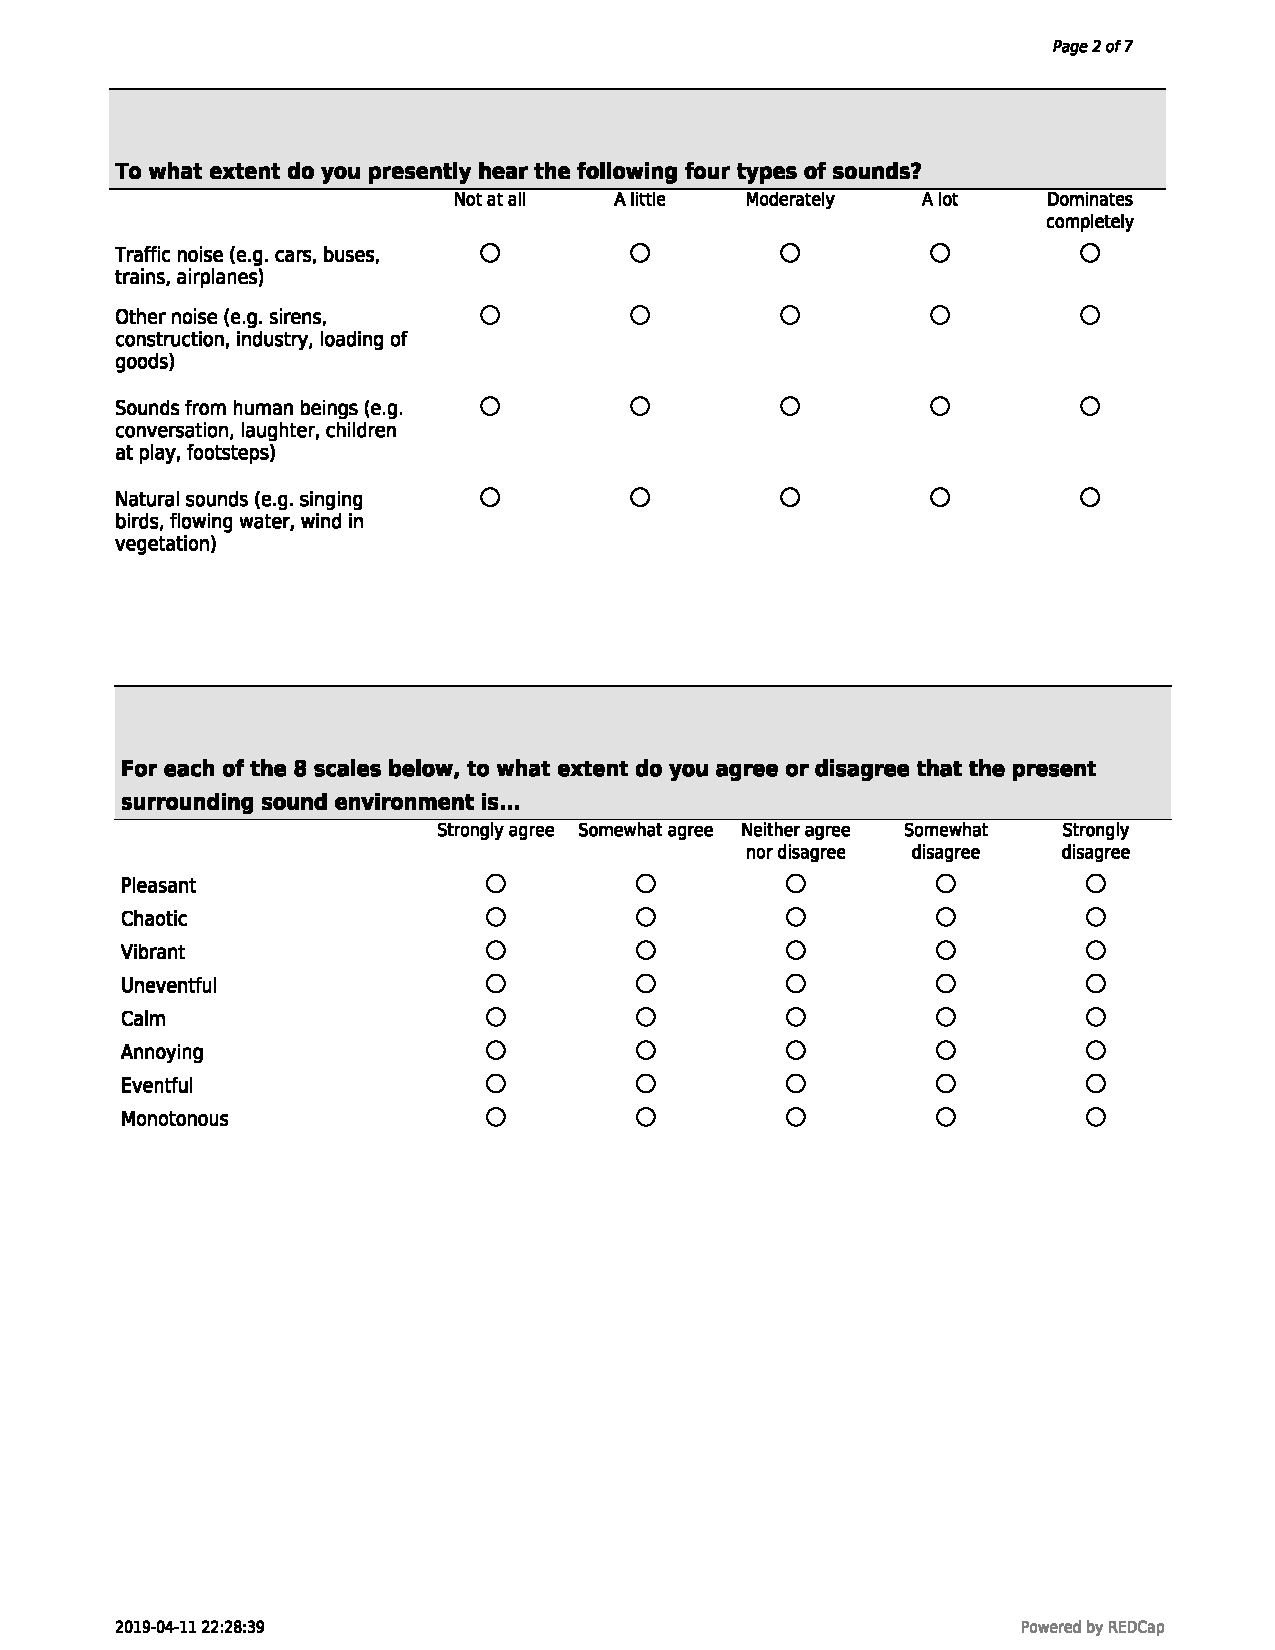
\includepdf[pages={1-5}]{./Papers/190411_LondonQuestionnaire_cutdown.pdf}

 \chapter{ISO 12913 Part 3 Report of Location Data}\label{app:location-data}
      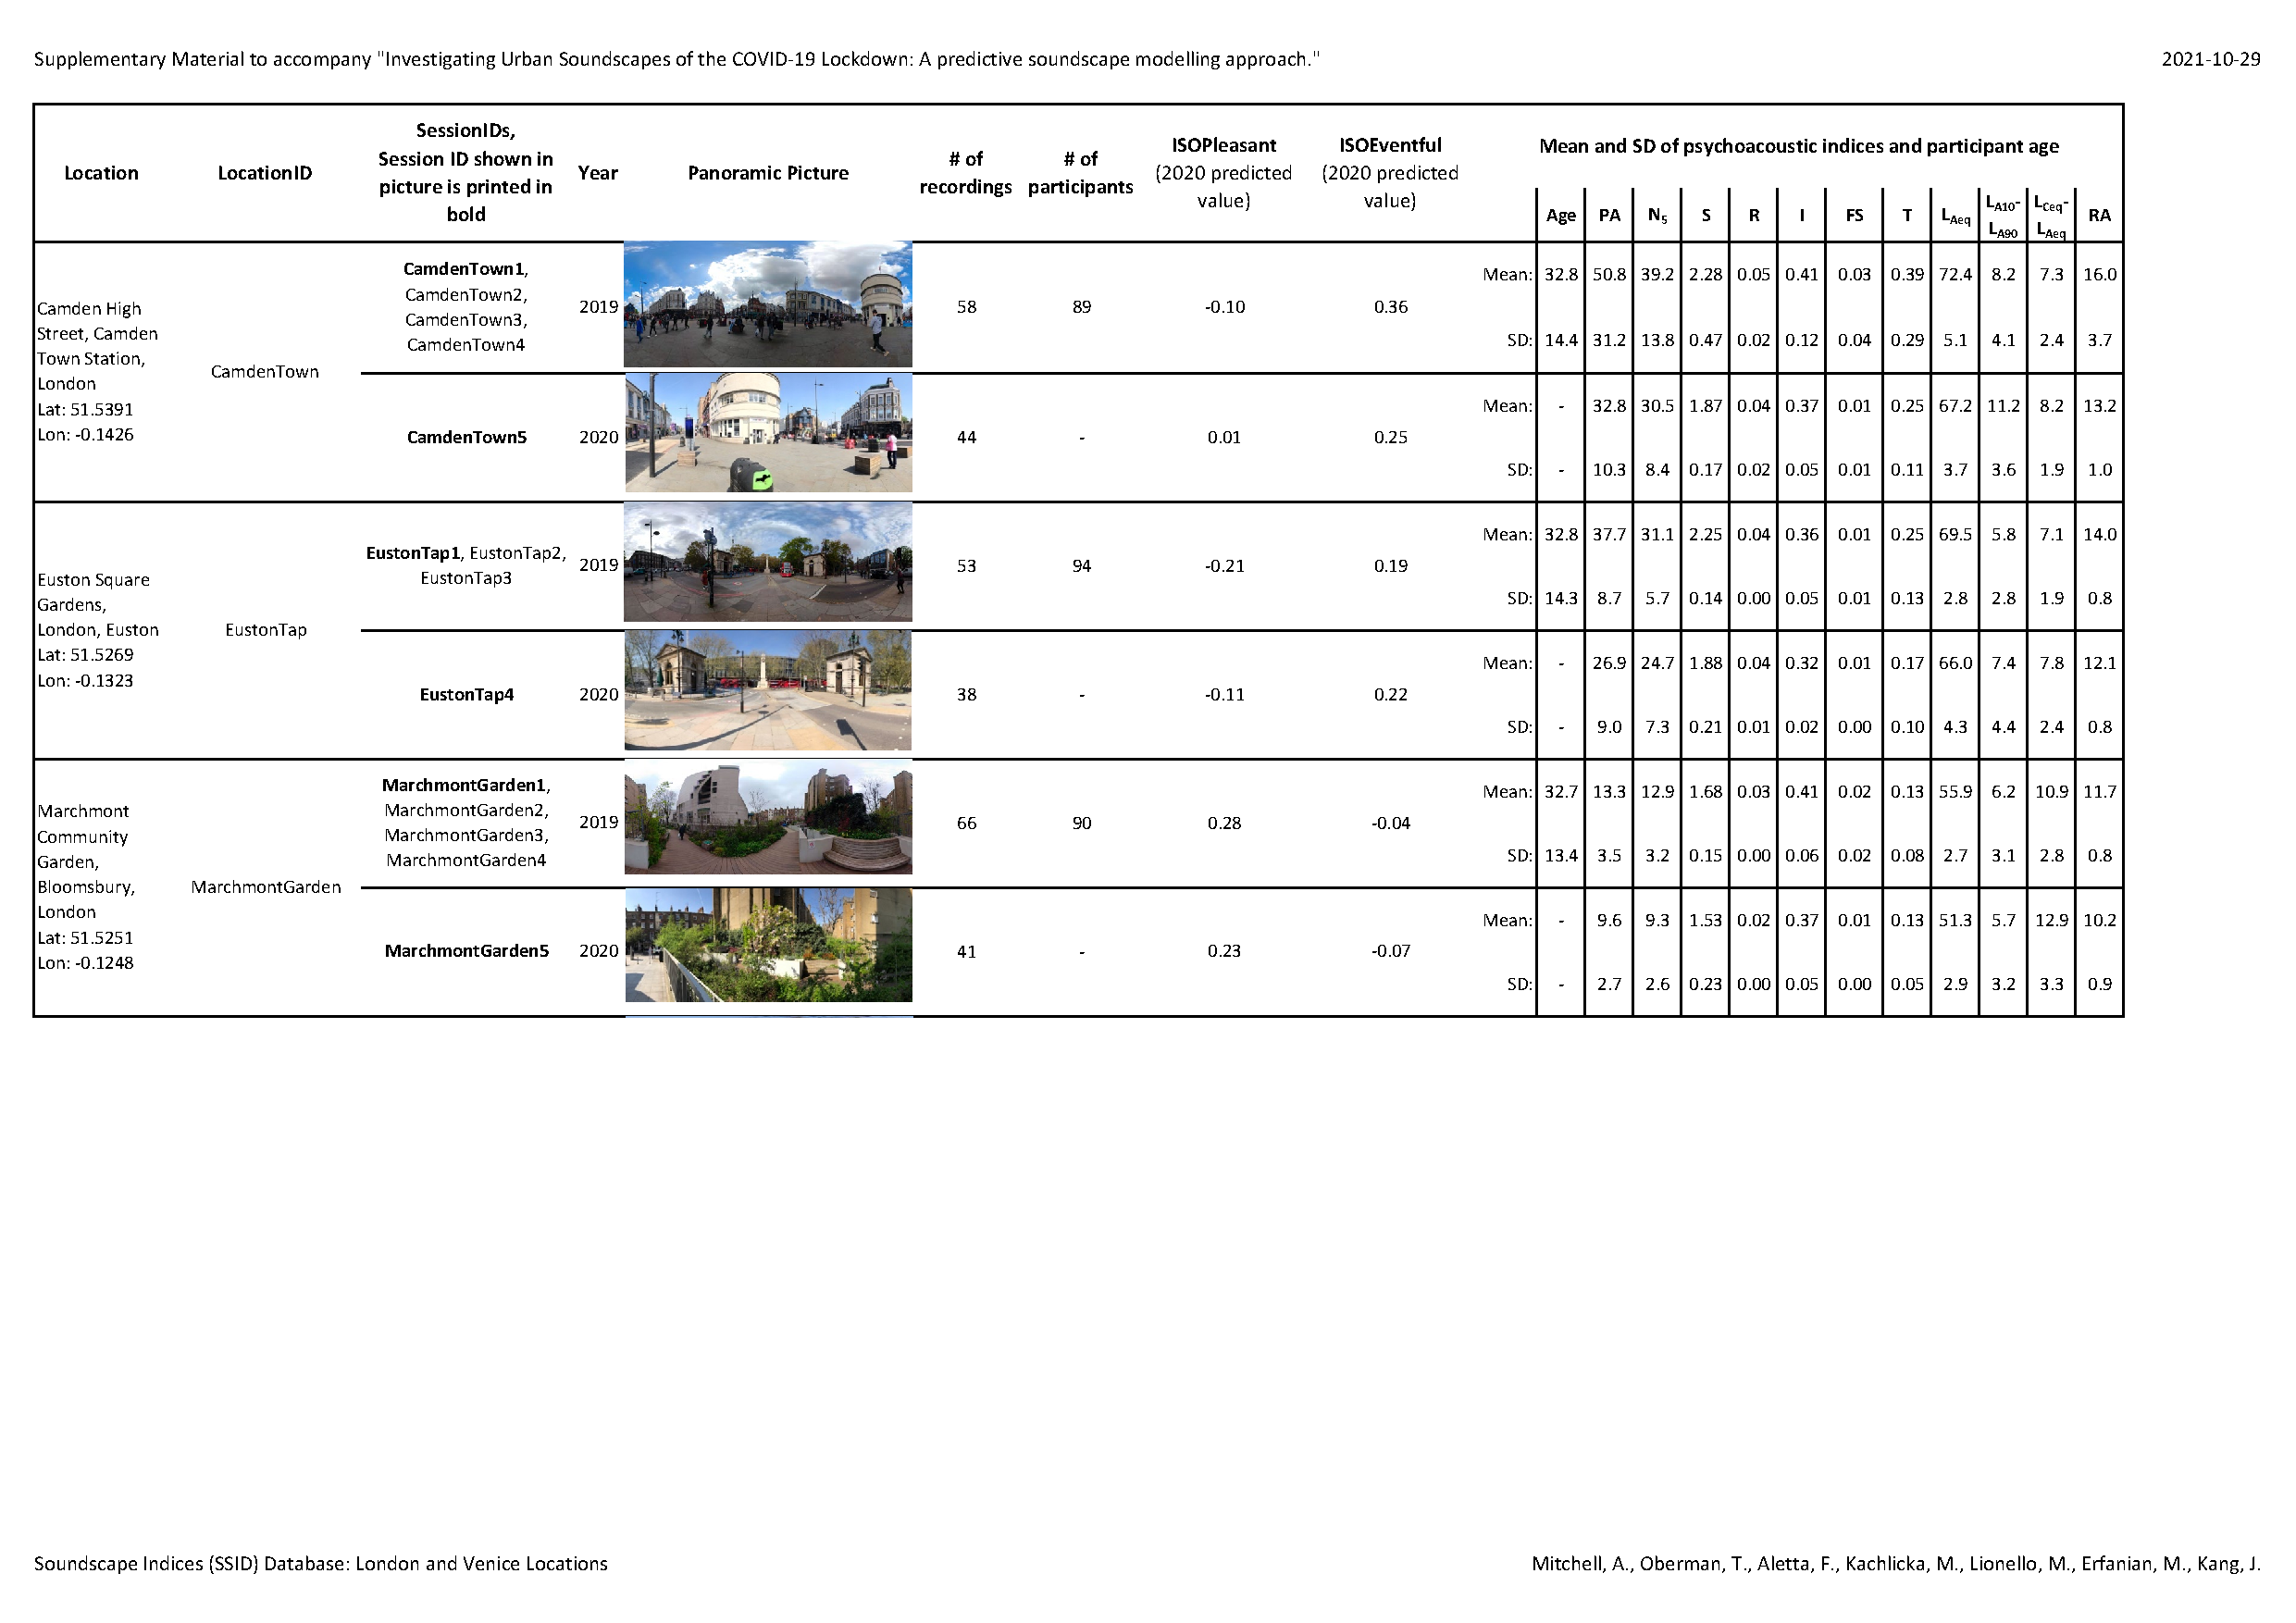
\includepdf[landscape=true,pages=1-4]{./Papers/SuppPub1-Location-data.pdf}

 \chapter{$1/f$ Analysis of complex sound environments}
\label{app:overf}

\draft{Massive edits to make}

\section{Abstract}

It has been proposed that the temporal structure of acoustic environments exhibit a $1/f^\alpha$ behaviour, like many other time series in nature. To investigate the relative randomness within urban soundscapes, the slope coefficient ($\alpha$) of the temporal structure of a series of psychoacoustic metrics is calculated for recordings made in ?15 locations across Europe. The first stage of this analysis involves identifying at which frequency regimes this $\alpha_{f}$ metric exhibits different behaviours for the various psychoacoustic metrics. Finally, the relationships between this temporal structure and the assessed soundscape pleasantness and eventfulness are examined and the most significant features are identified.

\section{Introduction}

\textbf{General justification for soundscape (no more than 3 sentences?).}
The impact of noise pollution on general health and well-being has been recognised for decades and various strategies have been developed to incorporate contributing effects on perception when considering the impact of the noise environment and have developed and improved tools for assessing the perceived quality of a sound environment, known as the soundscape.

The soundscape approach to assessing and addressing urban noise pollution aims to take a more holistic view of the sound environment than more traditional methods. This is typically done through in situ questionnaires, soundwalks, and interviews, as laid out recently in Section 5 of \citet{ISO12913Part2}.

\subsection{Perceptual Attributes}
The model of soundscape characterization described by Axelsson et al. \cite{Axelsson2010principal} and recently standardised by ISO 12913-2 \citep{ISO12913Part2} comprises 8 perceptual attributes. These perceptual attributes form a 2-dimensional circumplex axis in which Pleasant/Unpleasant is orthogonal to Eventful/Uneventful, which is subsequently 45\degree{} offset from the orthogonal axis containing Exciting/Monotonous
and Chaotic/Calm. Any measured soundscape can thus be plotted on the circumplex axis according to its rated perceptual attributes.

\subsection{Importance of temporal structure on the sound environment}

Previous work on identifying the key acoustic and psychoacoustic parameters has so far yielded conclusive results only in the realm of soundscape identification \cite{Rychtarikova2013Soundscape} and has indicated that traditional acoustic parameters and analysis are insufficient metrics for subjective assessment of a soundscape's overall pleasantness \cite{Aletta2014Towards}. However, progress has been made in determining the relationships between (psycho)acoustic parameters and more targeted perceptual attributes such as vibrancy and eventfulness \cite{Aletta2018Towards, Jeon2011Non}.


Over the years, attempts to improve or reform traditional methods of noise assessment have produced a multitude of available noise indicators. A vital subset of these have provided information regarding the time series of the acoustic environment, typically serving one or both of two primary purposes: (1) to generalise sound levels or the response to sound levels over an extended period of time, and (2) to indicate the amount of variability of the sound level over the time period.

Those which fall into only the first category includes 24 hour metrics such as Community Noise Equivalent Level (CNEL) and the Day-Night  or Day-Evening-Night Levels (L\textsubscript{dn}
and L\textsubscript{den}, respectively); also included are levels meant for work-safety assessments, such as Sound Exposure Level (SEL).
\draft{Note: Psychoacoustic metrics were developed for industrial assessments of single source, product noise. This limits their applicability to multi-source complex sounde environments. }
\draft{Discuss current methods of assessing urban noise, i.e. Leq, Ldn, SEL, Ln, and how they handle temporal structure. Discussion of statistical methods e.g. Venaklasen method for CALGreen?}
\draft{Discussion of perceptual attributes and their collection and uses. Relate perceptual attributes to acoustical metrics above. Any discussion of temporality in perceptual attributes?}


\subsubsection{Introduce and review items of previous research in the area (obligatory).}

\draft{Music and Self-organised criticality}
\cite{Jeon2011Non} investigated the idea of an overall temporal structure in music,

Key points:
\begin{itemize}
  \item Found a 1/f structure in the spectral density of fluctuations of the audio power of many musical selections and English speech.
  \item 1/f structure of audio power holds down to $5 * 10^{-4}$ Hz (2000s period).
  \item 1/f structure of frequency fluctuations of music holds down to the inverse to the length of the sample.
  \item 1/f structure of frequency fluctuations of English speech show different characteristics, with a break of around 0.1s, the length of a single syllable.
        \begin{quote}
          The spectral density $S_v(f)$ of a quantity $V(t)$ fluctuating with time $t$ is a \textbf{measure of the mean squared variation} $<V^2>$ in a unit bandwidth centered on the frequency $f$.
        \end{quote}


\end{itemize}


\citet{deCoensel20031f} were the first to investigate the presence of this $1/f$ structure in environmental sound sources. Using a selection of 6 recordings from quiet rural areas in Flanders, Belgium and 12 from urban spaces in Ghent, Belgium, the authors examine the log-log spectra of A-weighted sound pressure, psychoacoustic loudness, and pitch fluctuations (i.e. zero-crossing rate) of both rural and urban soundscapes.




\cite{Botteldooren2006temporal} presented a temporal indicator based on this \(1/f\) structure. However, ...

\citet{Yang2015Presence} investigated the presence of a $1/f^{\alpha}$ behaviour in 102 recordings made in the countryside, natural parks, and urban areas in England between 1994 and 2010. They extended the previous investigations beyond simply considering the $\alpha$ value, to also consider whether different frequency regimes (the authors use the term 'range' instead) demonstrated different behaviours and to include the quadratic deviation from the best-fitted straight line. By visual inspection of the $1/f$ plots of the various psychoacoustic metrics, the authors noted two breaks in the frequency regimes, at $10^{-1}$ Hz and at $10^0$ Hz

Through these three primary studies various approaches to understanding this behaviour in soundscapes have been advanced. However, as de Coensel, Botteldooren, and de Muer explicitly stated, none of them have attempted to "link our observations to perception of the soundscape by the human observer". This is where this study picks up.


\subsection{Justification}
Characterising the dynamic nature of the sound environment, and the influence this will have on perception, is key to extending our assessments beyond what can be assessed in person by researchers.

To bring soundscape back to its roots as a consideration of sound environments as akin to a musical composition, when considering and discussing a piece of music, the three primary components are Melody, Harmony, and Rhythm. In this way, we could consider melody as the foreground, sound mark, or keynote sounds; harmony as the background or ambient sound; and rhythm as the temporal structure of the sound environment, both of the foreground and background sounds. Although the first two domains are fairly well researched in the soundscape literature, there is a lack of understanding of the influence of temporal structure on perception in soundscape.

Rhythm and structure in music can be distinguished into several levels or domains: the short-term is the rhythm of individual notes; the medium-term is the rhythm and structure of musical phrases (which could include the repetition of short-term rhythms); the long-term is the overall structure of a piece and organisation of movements. In the same way, the temporal structure of a sound environment can be distinguished into several domains: short-term (10s?) being the time structure of individual sound events (e.g. repeated beeps or knocking); the medium-term ...

In order to move towards an understanding of the temporal structure of complex, real-world soundscapes and towards the eventual development of a metric to describe this temporal structure, an analysis of the $1/f^\alpha$ structures of urban soundscapes has been conducted. By drawing from the large Soundscape Indices (SSID) database \citep{Mitchell2020Soundscape}, which includes 1,600 socio-acoustic surveys and accompanying 30s binaural recordings characteristics of the $1/f^\alpha$ structure in the time series of calculated psychoacoustic metrics are identified. Correlations between this structure and the soundscape perception as assessed by the in-situ surveys are then calculated to identify the influence the temporal structure may have on perception in real-world urban soundscapes.

\subsection{Frequency ranges, intervals, and regimes}

zBZoth De Coensel and Yang identified frequency ranges or intervals over which the behaviour of the spectrum differs. \citet{deCoensel20031f} divided the frequency interval into two parts: $I_1 = [0.002 Hz, 0.2 Hz]$ and $I_2 = [0.2 Hz, 5 Hz]$. $I_1$ which ranges from 200ms to 5s is therefore taken to represents the behaviour of the source itself, while $I_2$, which ranges from 5s to 10min is influenced by behaviours \emph{between} sources.

If this hypothesis is correct, wherein the high frequency interval is \emph{within} sources and the low frequency interval is \emph{between} sources, we would then expect to see similar interval separation across several different metrics.


\section{Methods}
\subsection{Survey collection}

\paragraph{SSID Protocol} This study makes use of the database collected as part of the (SSID) project. This SSID database consists of soundscape assessments and corresponding recordings carried out in 17 locations across the United Kingdom, the Netherlands, Spain, and Italy. The \citet{ISO12913Part1} series was consulted for reporting on soundscape data. \citet{ISO12913Part2} and \citet{ISO12913Part3} were used as the basis of the data collection protocol and data analysis used. For a full description of the SSID Protocol and of the publicly available database, please see \citet{Mitchell2020Soundscape} and \citet{Mitchell2021Database}.

\subparagraph{Binaural Recorder}

\subparagraph{Sessions}

\paragraph{Sound sources and PAQ questions}

\section{Analysis}
The temporal variation of several psychoacoustic parameters has been analyzed for each of the included recordings. Based on previous soundscape literature \citep{yang}

\subsection{Recording Processing}
\paragraph{Psychoacoustic calc}

\subparagraph{Channel max}

\subsection{$1/f^\alpha$ Analysis}
\paragraph{Power Spectrum analysis} Welch's method for noisy signals. nperseg determination.
\paragraph{Slope ($\alpha$) calculation} Regression calculation for the given regimes.

\paragraph{Regime Breaks}

The regime break is defined as the point in the spectrum at which there is a noticeable change in the slope. This change indicates that the regime at frequencies below the break has a different $\alpha$ from the regime at frequencies above the break and therefore exhibits a different characteristic randomness behaviour.

Figure \ref{fig:regime_breaks} The spectra for all 1,000+ recordings is plotted, then the geometric mean line of these spectra is plotted in order to visualise the general pattern. The a mean line is used as it is otherwise impractical to investigate the behaviour across such a large number of samples. The geometric mean is used to account for the log scale relationship for the y-axis.



This is done for each parameter independently.

\subsection{Correlation Analysis}

Partial Distance Correlation using dcor package from Python. Or Mutual information. With control for SessionID.

\draft{Only explain the method of correlation analysis, leave justification (i.e. non-linear) for the results}


\section{Results \& Discussion}

\subsection{Identified time and frequency regimes}

\begin{figure}
  \centering
  % \includegraphics{}
  \caption{Set of plots including the average line for each of the parameters, with a dotted line indicating the identified regime break.}
  \label{fig:regime_breaks}
\end{figure}


\paragraph{Discuss} What does the regime above and below the break represent? How do we interpret this? How is it useful?

\subsection{Slope values}
\begin{figure}
  \centering
  % \includegraphics{}
  \caption{Single plot of a sample power spectrum, with the regression lines of the regimes plotted.}
  \label{fig:spectral_slope}
\end{figure}

\paragraph{Not -1 slope, not pink noise}

\begin{table}[]
  \centering
  \begin{tabular}{c|c}
     & \\
     &
  \end{tabular}
  \caption{Summary statistics of slopes?}
  \label{tab:my_label}
\end{table}

\paragraph{Discussion} Problems with using fft versus periodogram resulted in incorrect interpretation of previous results.


\section{Correlations}

\paragraph{Explain why MI is better for this.}

\begin{table}[]
  \centering
  \begin{tabular}{c|c|c|c|c|c}
    Rank & ISOPleasant & ISOEventful & Traffic & Natural & Human \\
    1    & SIL (.41)   & SIL (.43)   & ...     & ...     & ...   \\
    2    & ...         & ...         & ...     & ...     & ...   \\
  \end{tabular}
  \caption{Correlation rankings between psychoacoustic and temporal features, and perceptual features}
  \label{tab:my_label}
\end{table}

\begin{figure}
  \centering
  \caption{Non-linear scatterplot for highly correlated feature(s)}
  \label{fig:scatterplot}
\end{figure}

This is where the nrmse / deviation discussion / limitation can go.

\section{Concluding Remarks}

This theme appeared in literature 10 years ago, then just went quiet.



 \chapter{Deep Learning Techniques for the detection of noise Annoyance (DeLTA)}
\label{app:delta}

\end{appendices}

 %%%%%%%%%%%%%%%%%%%%%%%%%%%%%%%%%%%%%%%%%%%%%%%%%%%%%%%%%%%%%%%%%%%%%%%%%%%%%%%%%%%%%%%%%%%%%%%%%%

\end{document}
